% documentclass options:
\documentclass[11pt,
  a4paper,
  parskip=half, % This is some extra vertical space between paragraphs, the suggestion is 2cm which is really ugly, so we use what koma script gives us
  % you can also set it to full for even more space. But there is a bad tex style decision: parskip also changes the spacing between listitems such as
  % enumerate and itemize. For this purpose we include the enumitem package and set itemsep=.5em, of course you can change this
  BCOR=10mm, % BCOR is binding correction
  ngerman,
  % if you'd rather have a one sided thesis, add `oneside' to the documentclass
  oneside,
  % ngerman is needed for hyphenation if the thesis contains parts written in German, switch order with english if you write mainly in English.
  % Remember to change order in the babel package (below) as well.
  % Last language is the preferred one.
  english]{scrbook}
\usepackage[ngerman, english]{babel} % If you write mainly in English change order to ngerman, english. Also change that in the documentclass options above.
% Include of titling must happen before \title etc.
% that's why it's not in setup.tex
\usepackage{titling}
\title{Comparative Analysis of Load Balancing Algorithms in General Graphs}
\author{Emre Bayaz\i to\v{g}lu}

% Change to your first examiner
% The ~ enables non sentence spacing after a period
\newcommand{\firstexaminer}{Prof. Dr. Christian Schindelhauer}
% Change to your second examiner, some undergraduate studies don't have a second examiner
% in this case just comment out the following line

% Change to your adivers
\newcommand{\advisers}{Saptadi Nugroho}

% include all packages and define commands in setup.tex

%------------------------------------------------------------------------------
%       package includes
%------------------------------------------------------------------------------
    % font encoding is set up for pdflatex, for other environments see
    % http://tex.stackexchange.com/questions/44694/fontenc-vs-inputenc
    \usepackage[T1]{fontenc}  % 8-bit fonts, improves handling of hyphenations
    % provides `old' commands for table of contents. Eases the ability to switch
    % between book and scrbook
    \usepackage{scrhack}


    % ------------------- layout, default -------------------
    % adjust the style of float's captions, separated from text to improve readabilty
    \usepackage[labelfont=bf, labelsep=colon, format=hang, textfont=singlespacing]{caption}
    % With format = hang your caption will look like this:
    % Figure 1: Lorem ipsum dolor sit amet,
    %           consectetuer adipiscing elit.
    %           Ut purus elit, vestibulum
    % If you instead want
    % Figure 1: Lorem ipsum dolor sit amet,
    % consectetuer adipiscing elit. Ut purus
    % elit, vestibulum
    % change to format=plain
    \usepackage{chngcntr}  % continuous numbering of figures/tables over chapters
    \counterwithout{equation}{chapter}
    \counterwithout{figure}{chapter}
    \counterwithout{table}{chapter}

    % Uncomment the following line if you switch from scrbook to book
    % and comment the setkomafont line
    %\usepackage{titlesec}  % remove "Chapter" from the chapter title
    %\titleformat{\chapter}[hang]{\bfseries\huge}{\thechapter}{2pc}{\huge}
    \setkomafont{chapter}{\normalfont\bfseries\huge}

    \usepackage{setspace}  % Line spacing
    \onehalfspacing
    % \doublespacing  % uncomment for double spacing, e.g. for annotations in correction

    % ------------------- functional, default-------------------
    \usepackage[dvipsnames]{xcolor}  % more colors
    \usepackage{array}  % custom format per column in table - needed on the title page
    \usepackage{graphicx}  % include graphics
    \usepackage{subfig}  % divide figure, e.g. 1(a), 1(b)...
    \usepackage{amsmath}  % |
    \usepackage{amsthm}   % | math, bmatrix etc
    \usepackage{amsfonts} % |
    \usepackage{calc}  % calculate within LaTeX
    \usepackage[unicode=true,bookmarks=true,bookmarksnumbered=true,
                bookmarksopen=true,bookmarksopenlevel=1,breaklinks=false,
                pdfborder={0 0 0},backref=false,colorlinks=false]{hyperref}
    \usepackage{etoolbox} % if-else commands


    %==========================================
    % You might not need the following packages, I only included them as they
    % are needed for the example floats
    % ------------------- functional, custom -------------------
    \usepackage{algorithm,algpseudocode}
    \usepackage{bm}  % bold greek variables (boldmath)
    \usepackage{tikz}
    \usetikzlibrary{arrows,chains,positioning,scopes,quotes,bending,calc,intersections}  % use: above left of, etc
    
    % Required for the ToDo list.
    \usepackage{ifthen}

    % Improves general appearance of the text
    \usepackage[protrusion=true,expansion=true, kerning]{microtype}
    \usepackage{enumitem}
    % Nicer font for pdf rendering.
    %\usepackage{lmodern}
    
    % For nicer looking tables.
    \usepackage{multirow}

    % You don't need this, just for demonstration of a longer caption.
    \usepackage{lipsum}

    % for landscape mode
    \usepackage{adjustbox}

    % for hyperreference
    \usepackage{hyperref}



%------------------------------------------------------------------------------
%       (re)new commands / settings
%------------------------------------------------------------------------------
    % ----------------- referencing ----------------
    \newcommand{\secref}[1]{Section~\ref{#1}}
    \newcommand{\chapref}[1]{Chapter~\ref{#1}}
    \renewcommand{\eqref}[1]{Equation~(\ref{#1})}
    \newcommand{\figref}[1]{Figure~\ref{#1}}
    \newcommand{\tabref}[1]{Table~\ref{#1}}

    % ------------------- colors -------------------
    \definecolor{darkgreen}{rgb}{0.0, 0.5, 0.0}
    % Colors of the Albert Ludwigs University as in
    % https://www.zuv.uni-freiburg.de/service/cd/cd-manual/farbwelt
    \definecolor{UniBlue}{RGB}{0, 74, 153}
    \definecolor{UniRed}{RGB}{193, 0, 42}
    \definecolor{UniGrey}{RGB}{154, 155, 156}


    % ------------------- layout -------------------
    % prevents floating objects from being placed ahead of their section
    \let\mySection\section\renewcommand{\section}{\suppressfloats[t]\mySection}
    \let\mySubSection\subsection\renewcommand{\subsection}{\suppressfloats[t]\mySubSection}



    % ------------------- math formatting commands -------------------
    % define vectors to be bold instead of using an arrow
    \renewcommand{\vec}[1]{\mathbf{#1}}
    \newcommand{\mat}[1]{\mathbf{#1}}
    % tag equation with name
    \newcommand{\eqname}[1]{\tag*{#1}}


    % ------------------- pdf settings -------------------
    % ADAPT THIS
    \hypersetup{pdftitle={\thetitle},
                pdfauthor={\theauthor},
                pdfsubject={Undergraduate thesis at the Albert Ludwig University of Freiburg},
                pdfkeywords={deep learning, awesome algorithm,  undergraduate thesis},
                pdfpagelayout=OneColumn, pdfnewwindow=true, pdfstartview=XYZ, plainpages=false}


    %==========================================
    % You might not need the following commands, I only included them as they
    % are needed for the example floats

    % ------------------- Tikz styles -------------------
    \tikzset{>=latex}  % arrow style


    % ------------------- algorithm ---------------------
    % Command to align comments in algorithm
    \newcommand{\alignedComment}[1]{\Comment{\parbox[t]{.35\linewidth}{#1}}}
    % define a foreach command in algorithms
    \algnewcommand\algorithmicforeach{\textbf{foreach}}
    \algdef{S}[FOR]{ForEach}[1]{\algorithmicforeach\ #1\ \algorithmicdo}

    % line spacing should be 1.5
    \renewcommand{\baselinestretch}{1.5}

    % set distance between items in a list, for more details see the
    % enumitem package: https://www.ctan.org/pkg/enumitem
    \setlist{itemsep=.5em}
    
    % use ra in your tables to increase the space between rows
    % 1.3 should be fine
    \newcommand{\ra}[1]{\renewcommand{\arraystretch}{#1}}

	% ToDo counters
	\usepackage{ifthen} %für whiledo-Schleife
	\newcounter{todos}
	\setcounter{todos}{0}
	\newcounter{extends}
	\setcounter{extends}{0}
	\newcounter{drafts}
	\setcounter{drafts}{0}

	% ------------------- marker commands -------------------
    % ToDo command
    \newcommand{\todo}[1]{\textbf{\textcolor{red}{(TODO: #1)}}\refstepcounter{todos}\label{todo \thetodos}}
	\newcommand{\extend}[1]{\textbf{\textcolor{darkgreen}{(EXTEND: #1)}}\refstepcounter{extends}\label{extend \theextends}}
	% Lighter color to note down quick drafts
	\newcommand{\draft}[1]{\textbf{\textcolor{NavyBlue}{(DRAFT: #1)}}\refstepcounter{drafts}\label{draft \thedrafts}}
	
	% microtype with lmodern, see https://tex.stackexchange.com/questions/75305/microtype-warning-with-lmodern-package-and-koma-script
	%\DeclareMicrotypeAlias{lmss}{cmr}


\begin{document}
    \pagestyle{empty} % no header and no page number
    % disable hyper links to remove warning "destination with same identifier"
    % this means within this section nothing can be referenced with a hyperlink
    \hypersetup{pageanchor=false}

    % enable/disable, depending on your chosen language
    
\begin{titlepage}
\begin{center}

\newcommand{\HorizontalLine}{\rule{\linewidth}{0.3mm}}

{\Large Student Project Report}\\[1.3cm]


% _____________________________________________________________________________
\HorizontalLine \\[0.4cm]
% Write your title in a fancy way like this if you want to customize it, otherwise simply let tex do it for you
% \begin{spacing}{3}
%     {\huge \bfseries The Long, Long } \\
%     {\huge \bfseries Long Long} \\
%     {\huge \bfseries Title}\\
% \end{spacing}
{ \huge \bfseries \thetitle }
\HorizontalLine \\[1.5cm]
% _____________________________________________________________________________


{\Huge \theauthor} \\[2cm]


\begin{tabular}[hc]{>{\huge}l >{\huge}l}
  Examiner: & \firstexaminer \\[0.3cm]
  Adviser: & \advisers \\[1.2cm]
\end{tabular}
\vfill  % move the following text to the bottom

\Large {
    University of Freiburg\\
    Faculty of Engineering\\
    Department of Computer Science\\
    Chair of Computer Networks and Telematics\\[1cm]

    September 11\textsuperscript{th}, 2024\\
}
\end{center}
\end{titlepage}

\thispagestyle{empty}
% title page back
\ \vfill \ \\  % at least one space required before vfill
\
\
\textbf{Examiner}                  \smallskip{} \\
\firstexaminer                     \bigskip{} \\
\
% If there is a second examiner include it
\ifdef{\secondexaminer}
	{
	% Include
	\textbf{Second Examiner}       \smallskip{} \\
	\secondexaminer                \bigskip{} \\
	\
	}
	{
	% No second examiner, ignore
	}
\textbf{Adviser}                  \smallskip{} \\
\advisers


    \pagestyle{plain} % remove chapter name from top, page number at the bottom
    % use \pagestyle{headings} for having the chapter on top of the pages
    % if you wang a more fancy header use \usepackage[automark,headsepline]{scrlayer-scrpage}
    % and read about it in the KOMA script documentation, https://www.ctan.org/pkg/koma-script

    
    \frontmatter  % roman page numbers
    % Copied from the official declaration from the examination office (typos fixed).
% Please double check the wording on their website and report changes.
% (https://www.tf.uni-freiburg.de/de/studium-lehre/a-bis-z-studium/dokumente/Declarationforthefinalthesis.pdf)

\chapter*{Declaration}

I hereby declare that I am the sole author and composer of my thesis and that no other sources or learning aids, other than those listed, have been used. Furthermore, I declare that I have acknowledged the work of others by providing detailed references of said work.  \newline
I hereby also declare that my Thesis has not been prepared for another examination
or assignment, either wholly or excerpts thereof.
\\[3\normalbaselineskip]
\begin{tabular}{p{\textwidth/2} l}
  \rule{\textwidth/3}{0.4pt}   &   \rule{\textwidth/3}{0.4pt} \\
  Place, Date                  &   Signature
\end{tabular}

    \chapter*{Abstract}

In this work, we investigate the load balancing problem by comparing the Push-Pull Sum protocol proposed by Nugroho et al. \cite{nugroho2023PushPullSumDataAg} with the Single Proposal Load Balancing protocol introduced by Dinitz et al. \cite{dinitz2022localDealAgreementloadBalancing}. These protocols are designed for undirected graphs, where nodes transfer loads to their neighbors to achieve a balanced state across the network. The loads represent various computational tasks, such as CPU usage, memory utilization, or internet traffic. Balancing loads and therefore challenging over- and underloading helps improve the efficacy of distributed systems and prevent system and performance errors from occurring. In the context of cloud computing, such algorithms are important for reducing response times, ensuring system stability, and improving customer satisfaction.

To provide a comprehensive analysis, we implement the aforementioned load balancing algorithms and evaluate their performance through simulations. Simulations are conducted using the PeerSim simulation tool, where we compare the progression of the mean squared error across multiple computation rounds. The simulations are performed on various topologies with different characteristics to identify the limitations and strengths of each algorithm. For every topology, multiple simulations are conducted and then compared and analyzed.
    \tableofcontents
    \listoffigures
    \listoftables
    \listofalgorithms
    \hypersetup{pageanchor=true}  % re-enable hyperlinking

    \mainmatter  % Arabic page numbers
    \textbf{Keywords} Load balancing $\cdot$ General graph $\cdot$ Self-stabilization $\cdot$ Push-Pull Sum protocol $\cdot$ Single Proposal Deal-Agreement-Based protocol $\cdot$ Static graphs $\cdot$ Deterministic vs. randomized protocols $\cdot$ Peer-to-Peer networks

\renewcommand{\clearpage}{}
    \chapter{Introduction}\label{chap:introduction}
In the course of digitalisation, the efficient handling of data loads has become increasingly critical. Load balancing algorithms are utilized to combat over- and underloading of nodes in a undirected graph. The primary objective of these algorithms is to achieve a balanced state within the network, where the load on each node converges toward the average load of the entire network. 

This report examines two distinct load balancing algorithms across various network topologies and sizes. The first algorithm studied is the Push-Pull Sum protocol, introduced by Nugroho et al. \cite{nugroho2023PushPullSumDataAg}. The Push-Pull Sum protocol is a protocol, that combines the Push protocol \cite{kempe2003gossipbasedComp} with the Pull-Sum protocol. The Push-Pull Sum protocol is a randomized protocol. The Push-Pull Sum protocol is compared to the Single Proposal Load Balancing protocol proposed by Dinitz et al. \cite{dinitz2022localDealAgreementloadBalancing}. Unlike the Push-Pull Sum protocol the Single Proposal Load Balancing protocol is a deterministic load balancing algorithm. The Single Proposal Load Balancing algorithm is a deal-agreement-based algorithm, which means that every load transfer is based on a negotiation between the neighbors on how large the load transfer is going to be. To evaluate the performance of these algorithms, the Mean Squared Error (MSE) is employed as a metric, quantifying how far the network's current state deviates from the ideal, balanced state. A network is balanced if the MSE equals 0.

Load balancing is utilized in distributed systems such as cloud computing, where it is important to efficiently allocate ressources in order to reduce power consumption and improve execution times \cite{Aghdashi2022NovelDynamicLoadBalancing}. Particularly in customer-oriented domains, self-stabilization is a desirable property for load balancing algorithms. This property ensures that an algorithm can always achieve a balanced state, regardless of the initial state the network is in.

\textit{Contribution.} This report provides a comprehensive analysis of two distinct load balancing algorithms by comparing their performance in terms of Mean Squared Error (MSE) per round. Analysis are provided for simulations conducted across various network sizes and topologies, allowing us to get an insight into the strengths and limitations of each algorithm under different conditions. The simulations may be used to validate the properties and performance claims made in the original papers by Nugroho et al. \cite{nugroho2023PushPullSumDataAg} and Dinitz et al. \cite{dinitz2022localDealAgreementloadBalancing}.

\section{Problem Overview}
Consider a undirected graph of computers. Each computer in this undirected graph is assigned tasks and therefore has a computation load. To manage and balance these loads, computers can transfer tasks to or receive tasks from their neighboring computers, connected by edges in the graph.
In practice, while it is theoretically possible to transfer any amount of load across the edges, it is important to ensure that transfers do not contribute to imbalance in the network. Additionally, it is important to minimize the number of load transfers per node per round, as these operations are resource-intensive and can lead to inefficiencies if overused.

\section{Document Structure}
In the \hyperref[chap:background]{Algorithms and Concepts} chapter, we introduce the two load balancing algorithms as described in the referenced papers. This chapter also includes a detailed description of the simulation setup, under which the simulations are conducted (eg. number of rounds, simulation techniques...).

The tools and methodologies used for the simulations are discussed in the \hyperref[chap:simulations]{Simulations} chapter. Here, we introduce the chosen simulation tool, and provide implementation details aiming to contribute to a better understanding of the simulation results.

In the chapter \hyperref[chap:results]{Result and Evaluation of Simulations}, we present the simulation outcomes, including detailed descriptions of the topologies and an analysis of the results. This chapter concludes with a tabular summary highlighting the performance of each algorithm under different conditions.

Finally, the \hyperref[chap:appendix]{Appendix} contains additional simulation results, including those using powers of 10 instead of powers of 2, which are not covered in the main part of the report.

    \chapter{Algorithms and Concepts}\label{chap:background}
\renewcommand{\algorithmicrequire}{\textbf{Input:}}
\renewcommand{\algorithmicensure}{\textbf{Output:}}
\begin{algorithm}
\caption{Continuous Single-Proposal Deal-Agreement-Based protocol}\label{alg:DAB}
\begin{algorithmic}[1]
\Require An undirected graph $G=(V,E,load)$
\Ensure A load state with discrepancy at most $\epsilon$ on $G$
\For{$r=1$ and on}
\For{every node u}
\State Find a neighbor, $v$, with the minimal load
\If{$load_{r}(u) - load_{r}(v)>0$}
\State $u$ sends to $v$ a transfer proposal of value $(load_{r}(u)-load_{r}(v))/2$
\EndIf
\EndFor

\For{every node $u$}
\If{there is at least one transfer proposal to $u$}
\State Find a neighbor, $w$, proposing to $u$ the maximal transfer
\State Node $u$ makes a deal: informs node $w$ on accepting its proposal
\State The actual transfer from $w$ to $u$ is executed 
\EndIf
\EndFor

\For{every node $u$}
\State Node $u$ sends the updated value of its load to its neighbors
\EndFor
\EndFor
\end{algorithmic}
\end{algorithm}

\renewcommand{\algorithmicrequire}{\textbf{Input:}}
\renewcommand{\algorithmicensure}{\textbf{Output:}}
\begin{algorithm}
\caption{Push-Pull Sum Algorithm}\label{alg:PPS}
\begin{algorithmic}[1]
\Procedure{RequestData}{}
\State Chose a random neighbor node $v$
\State Send $(\frac{s_{u,t}}{2}, \frac{w_{u,t}}{2})$ to the chosen node $v$ and the node $u$ itself
\EndProcedure
\Procedure{ResponseData}{}
\State $R_{u,t} \leftarrow$ Set of the nodes calling $u$ at a round $t$
\For{\textbf{all} $i \in R_{u,t}$}
\State Reply to i with $\left( \frac{\frac{s_{u,t}}{2}}{|R_{u,t}|}, \frac{\frac{w_{u,t}}{2}}{|R_{u,t}|} \right)$
\EndFor
\EndProcedure
\Procedure{Aggregate}{}
\State $M_{u,t} \leftarrow \{(s_{m}, w_{m})\}$ messages sent to $u$ at a round $t-1$
\State $s_{u,t} \leftarrow \sum_{m \in M_{u,t}}^{}s_{m}, w_{u,t} \leftarrow\sum_{m \in M_{u,t}}^{}w_{m}$
\State $f_{avg} \leftarrow \frac{s_{u,t}}{w_{u,t}}$
\EndProcedure
\end{algorithmic}
\end{algorithm}

Simulations in this project were conducted with network sizes of up to $2^{14}$ nodes. Consequently, we required a simulation tool capable of handling such large network sizes for different topologies (also topologies with high connectivity, meaning a high number of edges in the graph). We selected PeerSim, a Java-based simulation tool, as it meets these requirements. PeerSim offers two simulation engines: the cycle-driven engine and the event-driven engine. We chose the cycle-driven model to compute the simulations for both protocols, since both protocols work in rounds.

\section{Setting}
Each simulation is run for 50 rounds. We use the \textit{continuous} versions of the protocols, allowing any load, not just integers, to be transferred across the edges. At the beginning of the simulations, the nodes are provided with the information of their own loads and a set of neighboring nodes (this is the input in the protocols). Load transfers can only happen in between rounds. The initial loads are uniformly distributed between 0 and 100. For each round of a simulation the mean squared error is computed. Both protocols are \textit{synchronous}, meaning that load transfers happen in a constant time. Different topologies are chosen. Simulations are conducted for following topologies:
\begin{itemize}
    \item complete graph
    \item star graph
    \item closed chain graph
    \item torus grid graph
    \item ring of cliques
    \item lollipop graph
\end{itemize}
These topologies have different properties, which lead to different simulation outcomes. For instance, the complete graph and the lollipop graph are characterized by high connectivity, which impacts the number of load transfers per round. Among the listed graphs there are also regular graphs, such as the ring of cliques, the torus grid graph, the closed chain graph or the complete graph for which the simulation of different network sizes is interesting, in order to investigate how this influences the outcomes.

\newcolumntype{C}[1]{>{\centering\arraybackslash}p{#1}}

\begin{table}[]
\centering
\begin{adjustbox}{
  addcode={\begin{minipage}{\width}
           \caption{Simulation Overview: conducted simulations per topology} \label{table:overviewsims}
}
          {\captionsetup{font=footnotesize}
           \caption*{* in \hyperref[chap:appendix]{Appendix}}
           \end{minipage}},
  rotate=90}
\begin{tabular}{|C{1cm}|C{2.5cm}|C{2cm}|C{2cm}|C{2cm}|C{3cm}|C{3cm}|C{3cm}|}\hline
\multicolumn{2}{|l|}{Network size}                      & Complete graph & Star graph & Closed Chain graph & Torus & Regular Ring of Cliques & Lollipop graph \\ \hline
\multicolumn{2}{|c|}{*$10^{1}$}              & \checkmark & \checkmark & \checkmark &  \text{\sffamily X} & \text{\sffamily X} & (5, 5) \checkmark \\ \hline
\multicolumn{2}{|c|}{*$10^{2}$}             & \checkmark & \checkmark & \checkmark & $10\times10$ \checkmark & $10\times10$ \checkmark & (50, 50) \checkmark  \\ \hline
\multicolumn{2}{|c|}{*$10^{3}$}            & \checkmark & \checkmark & \checkmark & \text{\sffamily X} & \text{\sffamily X} & (500, 500) \checkmark  \\ \hline
\multicolumn{1}{|c|}{\multirow{7}{*}{*$10^{4}$}} & \centering 10.000 & \checkmark               & \checkmark           & \checkmark                   & \checkmark      &               \checkmark  & \checkmark               \\ \cline{2-8} 
\multicolumn{1}{|c|}{} & \centering $100\times100$      & \text{\sffamily X} & \text{\sffamily X} & \text{\sffamily X} & \checkmark & \checkmark & \text{\sffamily X} \\ \cline{2-8} 
\multicolumn{1}{|c|}{} &  \centering$10\times1.000$      & \text{\sffamily X} & \text{\sffamily X} & \text{\sffamily X} & \checkmark & \checkmark & \text{\sffamily X} \\ \cline{2-8} 
\multicolumn{1}{|c|}{} & \centering $1.000\times10$      & \text{\sffamily X} & \text{\sffamily X} & \text{\sffamily X} & \checkmark & \checkmark & \text{\sffamily X} \\ \cline{2-8} 
\multicolumn{1}{|c|}{} & \centering $(5.000, 5.000)$ & \text{\sffamily X} & \text{\sffamily X} & \text{\sffamily X} & \text{\sffamily X} & \text{\sffamily X} & \checkmark \\ \cline{2-8} 
\multicolumn{1}{|c|}{} & \centering $(500, 9.500)$  & \text{\sffamily X} & \text{\sffamily X} & \text{\sffamily X} & \text{\sffamily X} & \text{\sffamily X} & \checkmark \\ \cline{2-8} 
\multicolumn{1}{|c|}{} & \centering $(9.500, 500)$  & \text{\sffamily X} & \text{\sffamily X} & \text{\sffamily X} & \text{\sffamily X} & \text{\sffamily X} & \checkmark \\ \hline
% powers of 2
\hline
\multicolumn{2}{|c|}{$2^{4}$}              & \checkmark & \checkmark & \checkmark &  $4\times4$ \checkmark & $4\times4$ \checkmark & (8, 8) \checkmark \\ \hline
\multicolumn{2}{|c|}{$2^{8}$}             & \checkmark & \checkmark & \checkmark &  $16\times16$ \checkmark & $16\times16$ \checkmark & (128, 128) \checkmark  \\ \hline
\multicolumn{2}{|c|}{$2^{12}$}            & \checkmark & \checkmark & \checkmark & $64\times64$ \checkmark & $64\times64$ \checkmark & (2048, 2048) \checkmark  \\ \hline
\multicolumn{1}{|c|}{\multirow{4}{*}{$2^{14}$}} & \centering 16.384 & \checkmark               & \checkmark           & \checkmark                   & \checkmark      &               \checkmark  & \text{\sffamily X}               \\ \cline{2-8} 
\multicolumn{1}{|c|}{} & \centering $128\times128$      & \text{\sffamily X} & \text{\sffamily X} & \text{\sffamily X} & \checkmark & \checkmark & \text{\sffamily X} \\ \cline{2-8} 
\multicolumn{1}{|c|}{} & \centering $32\times512$      & \text{\sffamily X} & \text{\sffamily X} & \text{\sffamily X} & \checkmark & \checkmark & \text{\sffamily X} \\ \cline{2-8} 
\multicolumn{1}{|c|}{} & \centering $512\times32$      & \text{\sffamily X} & \text{\sffamily X} & \text{\sffamily X} & \checkmark & \checkmark & \text{\sffamily X} \\ \cline{2-8}  \hline
\end{tabular}
\end{adjustbox}
\end{table}

\section{Deal-Agreement-Based Protocol}
Algorithm \ref{alg:DAB} illustrates the continuous version of the load balancing protocol proposed in the paper by Dinitz et al. \cite{dinitz2022localDealAgreementloadBalancing}. This protocol is divided into three phases, namely the "proposal"-phase, the "deal"-phase and the "summary"-phase.
\begin{itemize}
    \item \textbf{Proposal}: In this phase every node is instructed to propose a \textit{fair} proposal to its neighbor with the minimal load. A proposal from node $u$ to node $v$ in round $r$ is considered fair if the proposed transfer amount $l$ satisfies $l \leq \frac{load_{r}(u) - load_{r}(v)}{2}$.
    \item \textbf{Deal}: Now, the nodes evaluate the proposal and accept the load transfer with the maximal proposing node.
    \item \textbf{Summary} This is the last phase. The nodes inform their neighbors about their updated values after the load transfer happened.
\end{itemize}
This approach is a deterministic approach, there is no element of random involved. We need to keep this in mind when looking into the simulations later on in chapter \ref{chap:simulations}, as achieving good results with deterministic protocols can often be more challenging compared to randomized ones. Additionally, this protocol is considered an \textit{anytime} protocol. We could therefore stop the simulation at any time, regardless of the initial state of the network, and the state of the network would not worsen at any step of the simulation. The protocol is designed to produce a "load state with discrepancy at most $\epsilon$ on $G$," where $\epsilon$ represents an arbitrarily small bound on the final discrepancy \cite{dinitz2022localDealAgreementloadBalancing}. The \textit{discrepancy} is the difference between the maximum load and the minimum load of the network. As initial information this protocol takes in a undirected graph $G$ with all the nodes, edges (interconnection of the nodes) and their respective loads.

\section{Push-Pull-Sum Protocol}
The Push-Sum protocol, as proposed in the paper by Kempe et al. \cite{kempe2003gossipbasedComp}, is a load balancing protocol where each node selects a random neighbor and transfers half of its current sum and weight to that neighbor. The Push-Pull-Sum protocol is composed of the Push-Sum and the Pull-Sum protocol. Upon a push action the calling node (the "caller") sends a pull request to the called node (the "callee"), which results in the callee to send its sum and weight divided by the number of pull requests to the caller and to itself \cite{nugroho2023PushPullSumDataAg}.

Consequently, a push operation of round $r$ is a load transfer of the caller to the callee of $\left(\frac{s_{r}}{2}, \frac{w_{r}}{2}\right)$ and itself. And a pull operation is a load transfer of the callee to the callers of values $\left(\frac{\frac{s_{r}}{2}}{|R|}, \frac{\frac{w_{r}}{2}}{|R|}\right)$ to each caller and itself.

The implementation of the Push-Pull Sum protocol is subdivided into three procedures:
\begin{itemize}
    \item \textbf{Aggregate}: In this procedure every node counts the number of ingoing messages, sent by their neighbors to them. The messages sent to a node are aggregated. Following that, the node calculate its sum and weight and computes the average $f_{avg} = \frac{s_{u, r}}{w_{u, r}}$.
    \item \textbf{RequestData}: After aggregating the data, each node randomly selects a neighbor and executes a push operation to this neighbor and to itself.
    \item \textbf{ResponseData}: In this procedure, each node accumulates all pull requests received during the round into a set $R_{u, r}$. For every request in this set, a pull operation is executed, sending the node's sum and weight to the requesting nodes and updating the node's own values.
\end{itemize}
In the beginning of every round (except the first round - since there is nothing to aggreagate) the \textit{aggregate} procedure is called. Following that the \textit{RequestData} procedure is called. Finally, at the end of each round the \textit{responseData} is called. We can observe that the sum of all weights at any round is equal to the networksize. Unlike the Deal-Agreement-Based protocol, the Push-Pull-Sum protocol is no deterministic protocol, but a randomized protocol.
    \chapter{Simulations}\label{chap:simulations}
In this chapter, we describe the setup and execution of the simulations used to evaluate the load balancing algorithms. Simulations are conducted using the PeerSim simulation tool for Java. Different topologies are implemented. For every simulation a output file is generated containing, the loads, sums and weights of every node per round and the mean squared error of the graph per round. Also the configuration files contain information regarding the setting of the simulation, like the network size or the topology chosen for the simulation. These output files are processed and analyzed using Python, with \textit{Matplotlib}, as it provides a variety of options for plotting and a comprehensive and detailed documentation.

\section{PeerSim}
PeerSim is a simulation tool developed for the Java programming language. PeerSim is composed of two engines: the event-driven engine and the cycle-driven engine. We chose the cycle-driven engine for our simulations. PeerSim is specifically designed for large-scale network simulations due to its high scalability and the ability to program with pluggable components. A PeerSim simulation generally follows four main steps:
\begin{enumerate}
    \item \textbf{Configuration file creation}: The simulation begins with the creation of a configuration file that defines the simulation parameters. This file specifies the network size, the protocols to be used, and other necessary settings.
    \item \textbf{Protocol selection}: After the configuration step, the next step is to choose the protocol or protocols to be simulated. This can involve running multiple protocols in parallel or focusing on a single protocol.
    \item \textbf{Control object selection}: Now, it is time to initialize control objects to monitor simulation parameters. Our control objects are classes named \textit{<Protocol>Observer}.
    \item \textbf{Simulator class invoking}: Lastly, the configuration file has to be invoked by the peersim.Simulator class \cite{peersimdocs}. For that, the IDE is instructed to call the simulator class on click of the "run"-button. Alternatively, a command line in the terminal can also invoke the simulator class. More on this in the \hyperref[https://peersim.sourceforge.net/]{PeerSim docs}.
\end{enumerate}
PeerSim is a simulation tool developed in Java, that provides many classes and interfaces for simulation. For the cycle-driven approach a interface \textit{CDProtocol} is provided by the simulation framework, which provides the \textit{nextCycle} method. The \textit{nextCycle} method is executed in the beginning of every round.

Nodes in PeerSim are implemented as containers that hold various protocols. Every node is identified by an ID and interacts with the \textit{Linkable} interface, which provides us with access to the neighboring protocols. A class that implements the \textit{Linkable} interface, may override different methods, like the \textit{getNeighbor} method, which retrieves a neighbor with a specified ID. The \textit{degree} method, returns the number of neighbors a node has. A method \textit{addNeighbor}, adds a neighbor to a node's set of neighbors. To monitor and modify the simulations control objects are required. A class implementing the \textit{Control} interface includes the \textit{execute} method. This method can be used to observe or alter the simulation at each round cite{peersimdocs}.

\section{Implementation Details}
Both implementations of the algorithms are composed of at least two different java classes: an observer class and a protocol class. Additionally, a shared parameter class, named \textit{LoadBalancingParameters.java}, is utilized by all protocols for storing shared parameters (e.g. the round number or the dimensions of specific graphs). Protocol-specific parameters are managed within their respective protocol classes. The observer class of a protocol handles the implementation and the monitoring of the protocols. The implementation of the topologies is also handled in the observer classes. To generate a link between two nodes, we simply add the node ID to the node's set of neighbors. Since we are in a static setting, the links are created during round 0, which is dedicated to initialization tasks. The output files are generated on-the-fly, while simulating. At the end of each round the mean squared error values are appended to the output file.

    \chapter{Result and Evaluation of Simulations}\label{chap:results}
In the following the simulations are presented for the different topologies. The networksizes chosen for the simulations are to the base 2. For an overview of the conducted simulations, one can refer to table \ref{table:overviewsims}. We also conducted simulations to the base 10, which one can find in the \hyperref[chap:appendix]{Appendix}.
The graph is a so-called \textit{log-log graph}, meaning that we have logarithmic scales for both, the x-axis showing the number of rounds and the y-axis representing the scale for the mean squared error. The Single-Proposal-Deal-Agreement-Based algorithm is abbreviated in the following as \textit{DAB}, while the Push-Pull Sum algorithm is abbreviated as \textit{PPS}. In each subsection a winner is singled-out. The Simulations

\section{Complete Graphs}
\textbf{The Complete graph}: The complete graph as depicted in \hyperref[fig:completegraphDemo]{figure} \ref{fig:completegraphDemo} is a graph where each pair of distinct nodes is connected by an edge. The complete graph contains of $n$ nodes and $\frac{n\times(n-1)}{2}$ edges. Every node has a degree of $n-1$, since each node is connected to every other node except to itself \cite{GraphTheorySchindelhaauer2021}. The complete graph is a dense graph, since it has the maximal amount of edges for a given number of nodes.
\begin{figure}
    \centering
    \begin{tikzpicture}
    \foreach \i in {1,...,16} {
      \node[draw, fill=blue, circle, minimum size=6pt] (v\i) at ({360/16 * (\i-1)}:4) {};
    }
    
    \foreach \i in {1,...,16} {
      \foreach \j in {1,...,16} {
        \ifnum\i<\j
          \draw (v\i) -- (v\j);
        \fi
      }
    }
    
  \end{tikzpicture}
    \caption{Complete graph: network size 16}
    \label{fig:completegraphDemo}
\end{figure}
\subsection{Network Size 2\textsuperscript{4}}
\textbf{Analysis}: The plot of figure \ref{fig:16CompleteGraph} indicates that the MSE of the network balanced by the DAB algorithm does not initially fall as significantly compared to the PPS. In round 29, the MSE suddenly manages to reduce the error of the network to 0. An MSE of 0 suggests a balanced network. All nodes have the same load. This is exactly the state we are aiming for. Despite the initially steeper downward slope of the PPS graph, the DAB ultimately manages to balance the graph more quickly. The remaining simulation showed that in some cases the DAB protocol reduces the error of the network faster, however there are cases like in the \hyperref[chap:appendix]{Appendix} where the PPS performs better for small network sizes. \\
The number of edges for a network size of 16 is 120. The PPS chooses its load transfer by random. For the PPS each load transfer step involves a push and a pull operation. For a small network size the PPS cannot already exploit the high connectivity of the graph. With increasing network change the PPS will perform better as we see. On the other hand, it is possible for the DAB algorithm to fully balance the network within 50 rounds, since each load transfer involves the maximal possible fair load. \\
\textbf{Winner}: DAB/PPS\\
\begin{figure}[H]
    \centering
    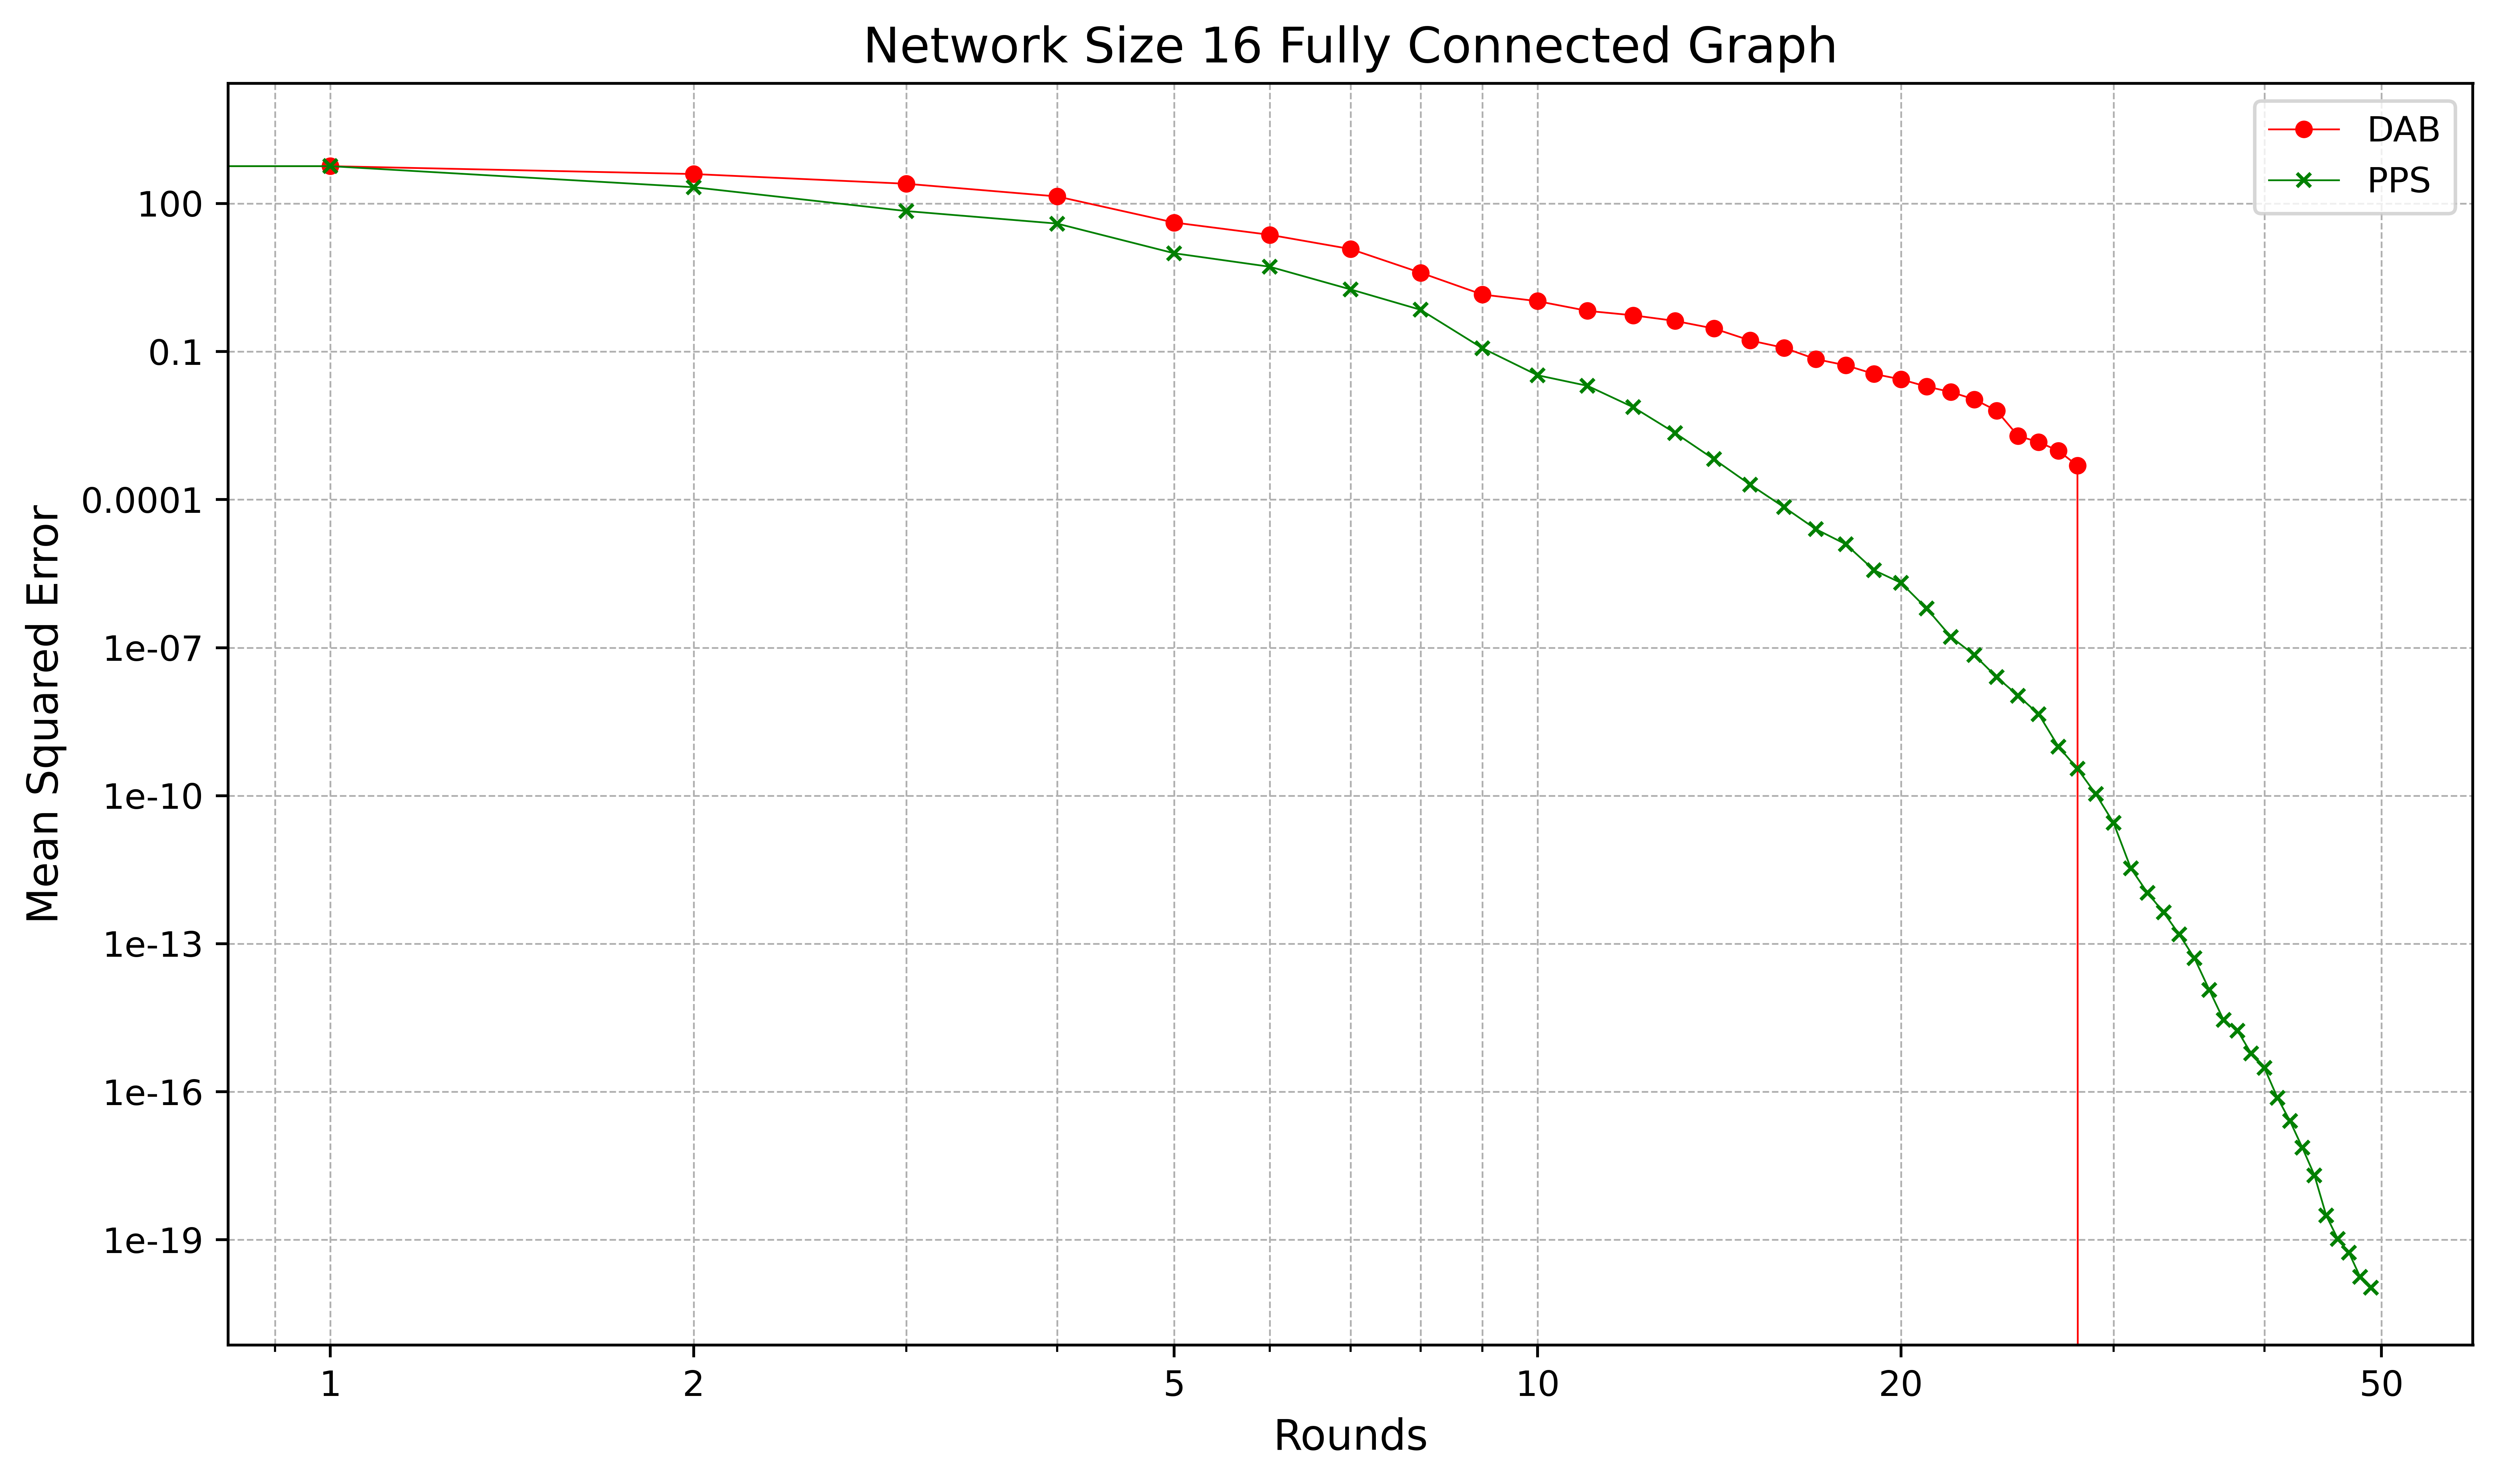
\includegraphics[scale=0.5]{figures/completeGraphSimulations/DAB_vs_PPS_FCG_r50_n16.png}
    \caption{Fully connected graph: network size $2^{4}$ nodes}
    \label{fig:16CompleteGraph}
\end{figure}

\subsection{Network Sizes 2\textsuperscript{8}, 2\textsuperscript{12}, 2\textsuperscript{14}}
\textbf{Analysis}: For bigger network sizes PPS outperforms DAB. The plots of figures \ref{fig:256CompleteGraph}, \ref{fig:4096CompleteGraph} and \ref{fig:16384CompleteGraph} indicate this very clearly. The plots show that DAB maintains a consistent MSE of the network of around 1,000 across all rounds, indicating that it does not improve (or change) significantly over time. PPS, on the other hand reaches a significant decrease in MSE as the number of rounds increases, indicating that PPS improves a lot better than DAB with more rounds and achieves a much lower error, reaching down to less than $1e-14$.\\
\textbf{Winner}: PPS
\begin{figure}[H]
    \centering
    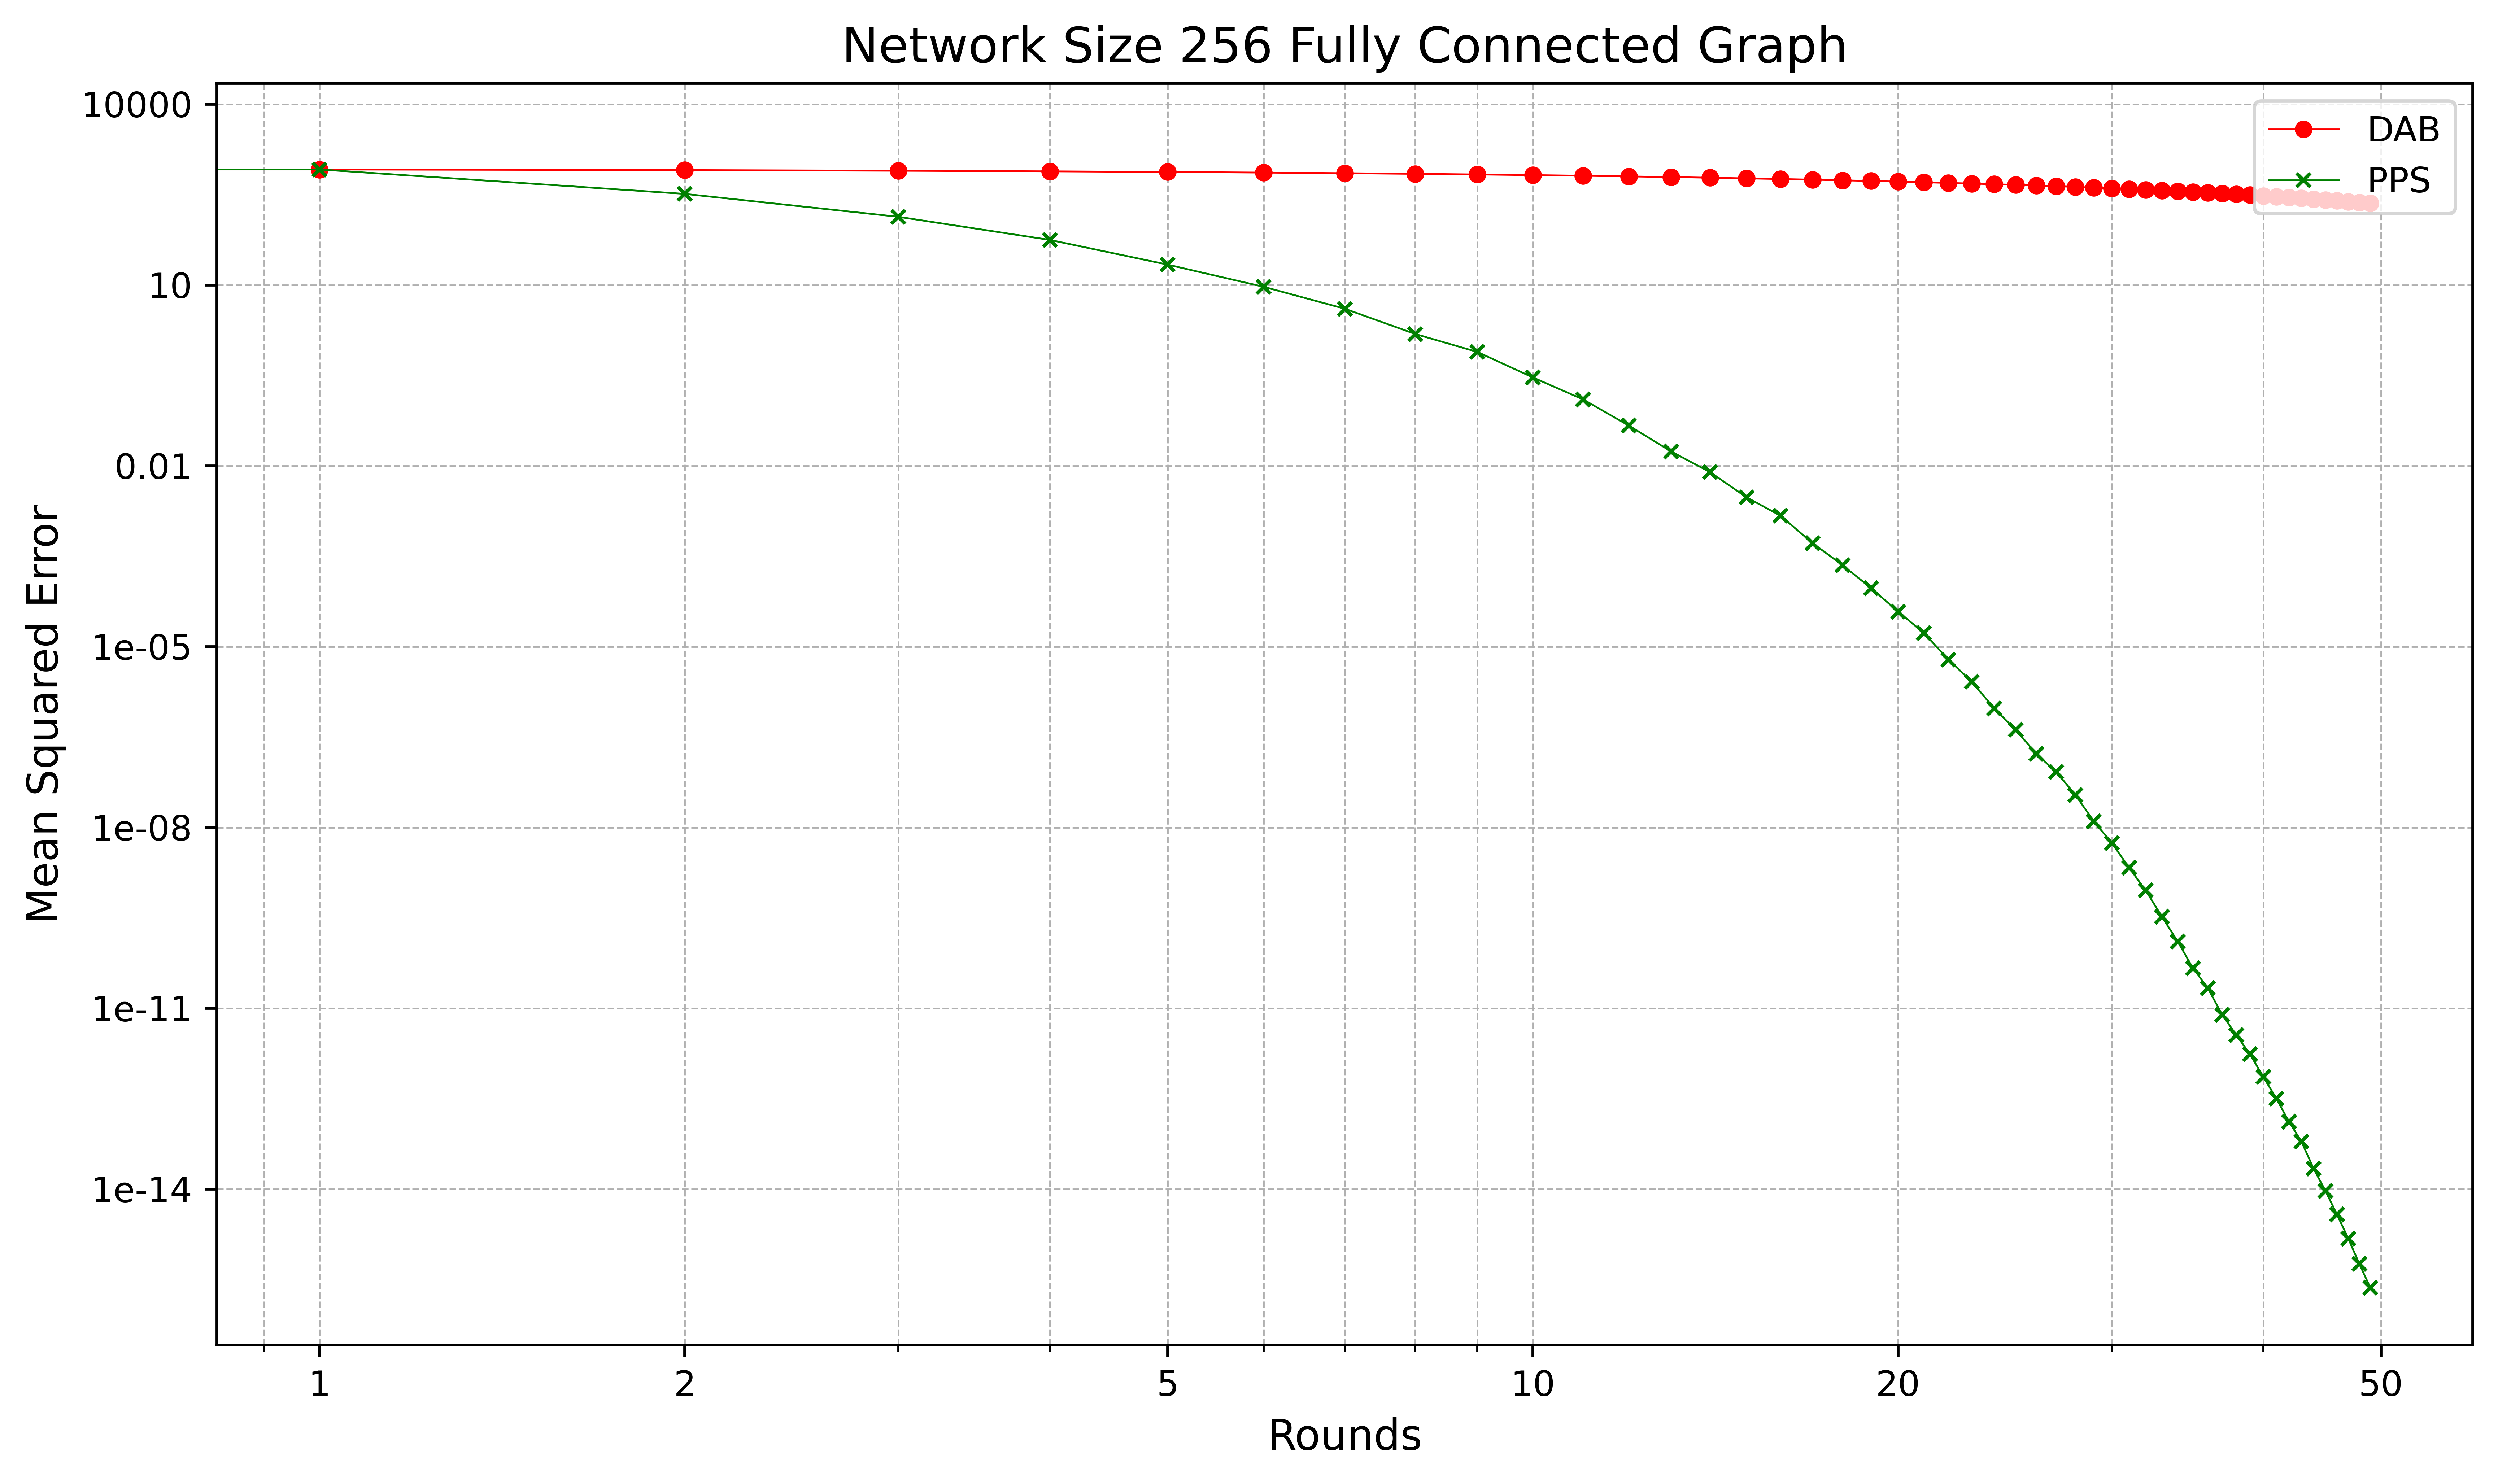
\includegraphics[scale=0.5]{figures/completeGraphSimulations/DAB_vs_PPS_FCG_r50_n256.png}
    \caption{Fully connected graph: network size $2^{8}$ nodes}
    \label{fig:256CompleteGraph}
\end{figure}

\begin{figure}[H]
    \centering
    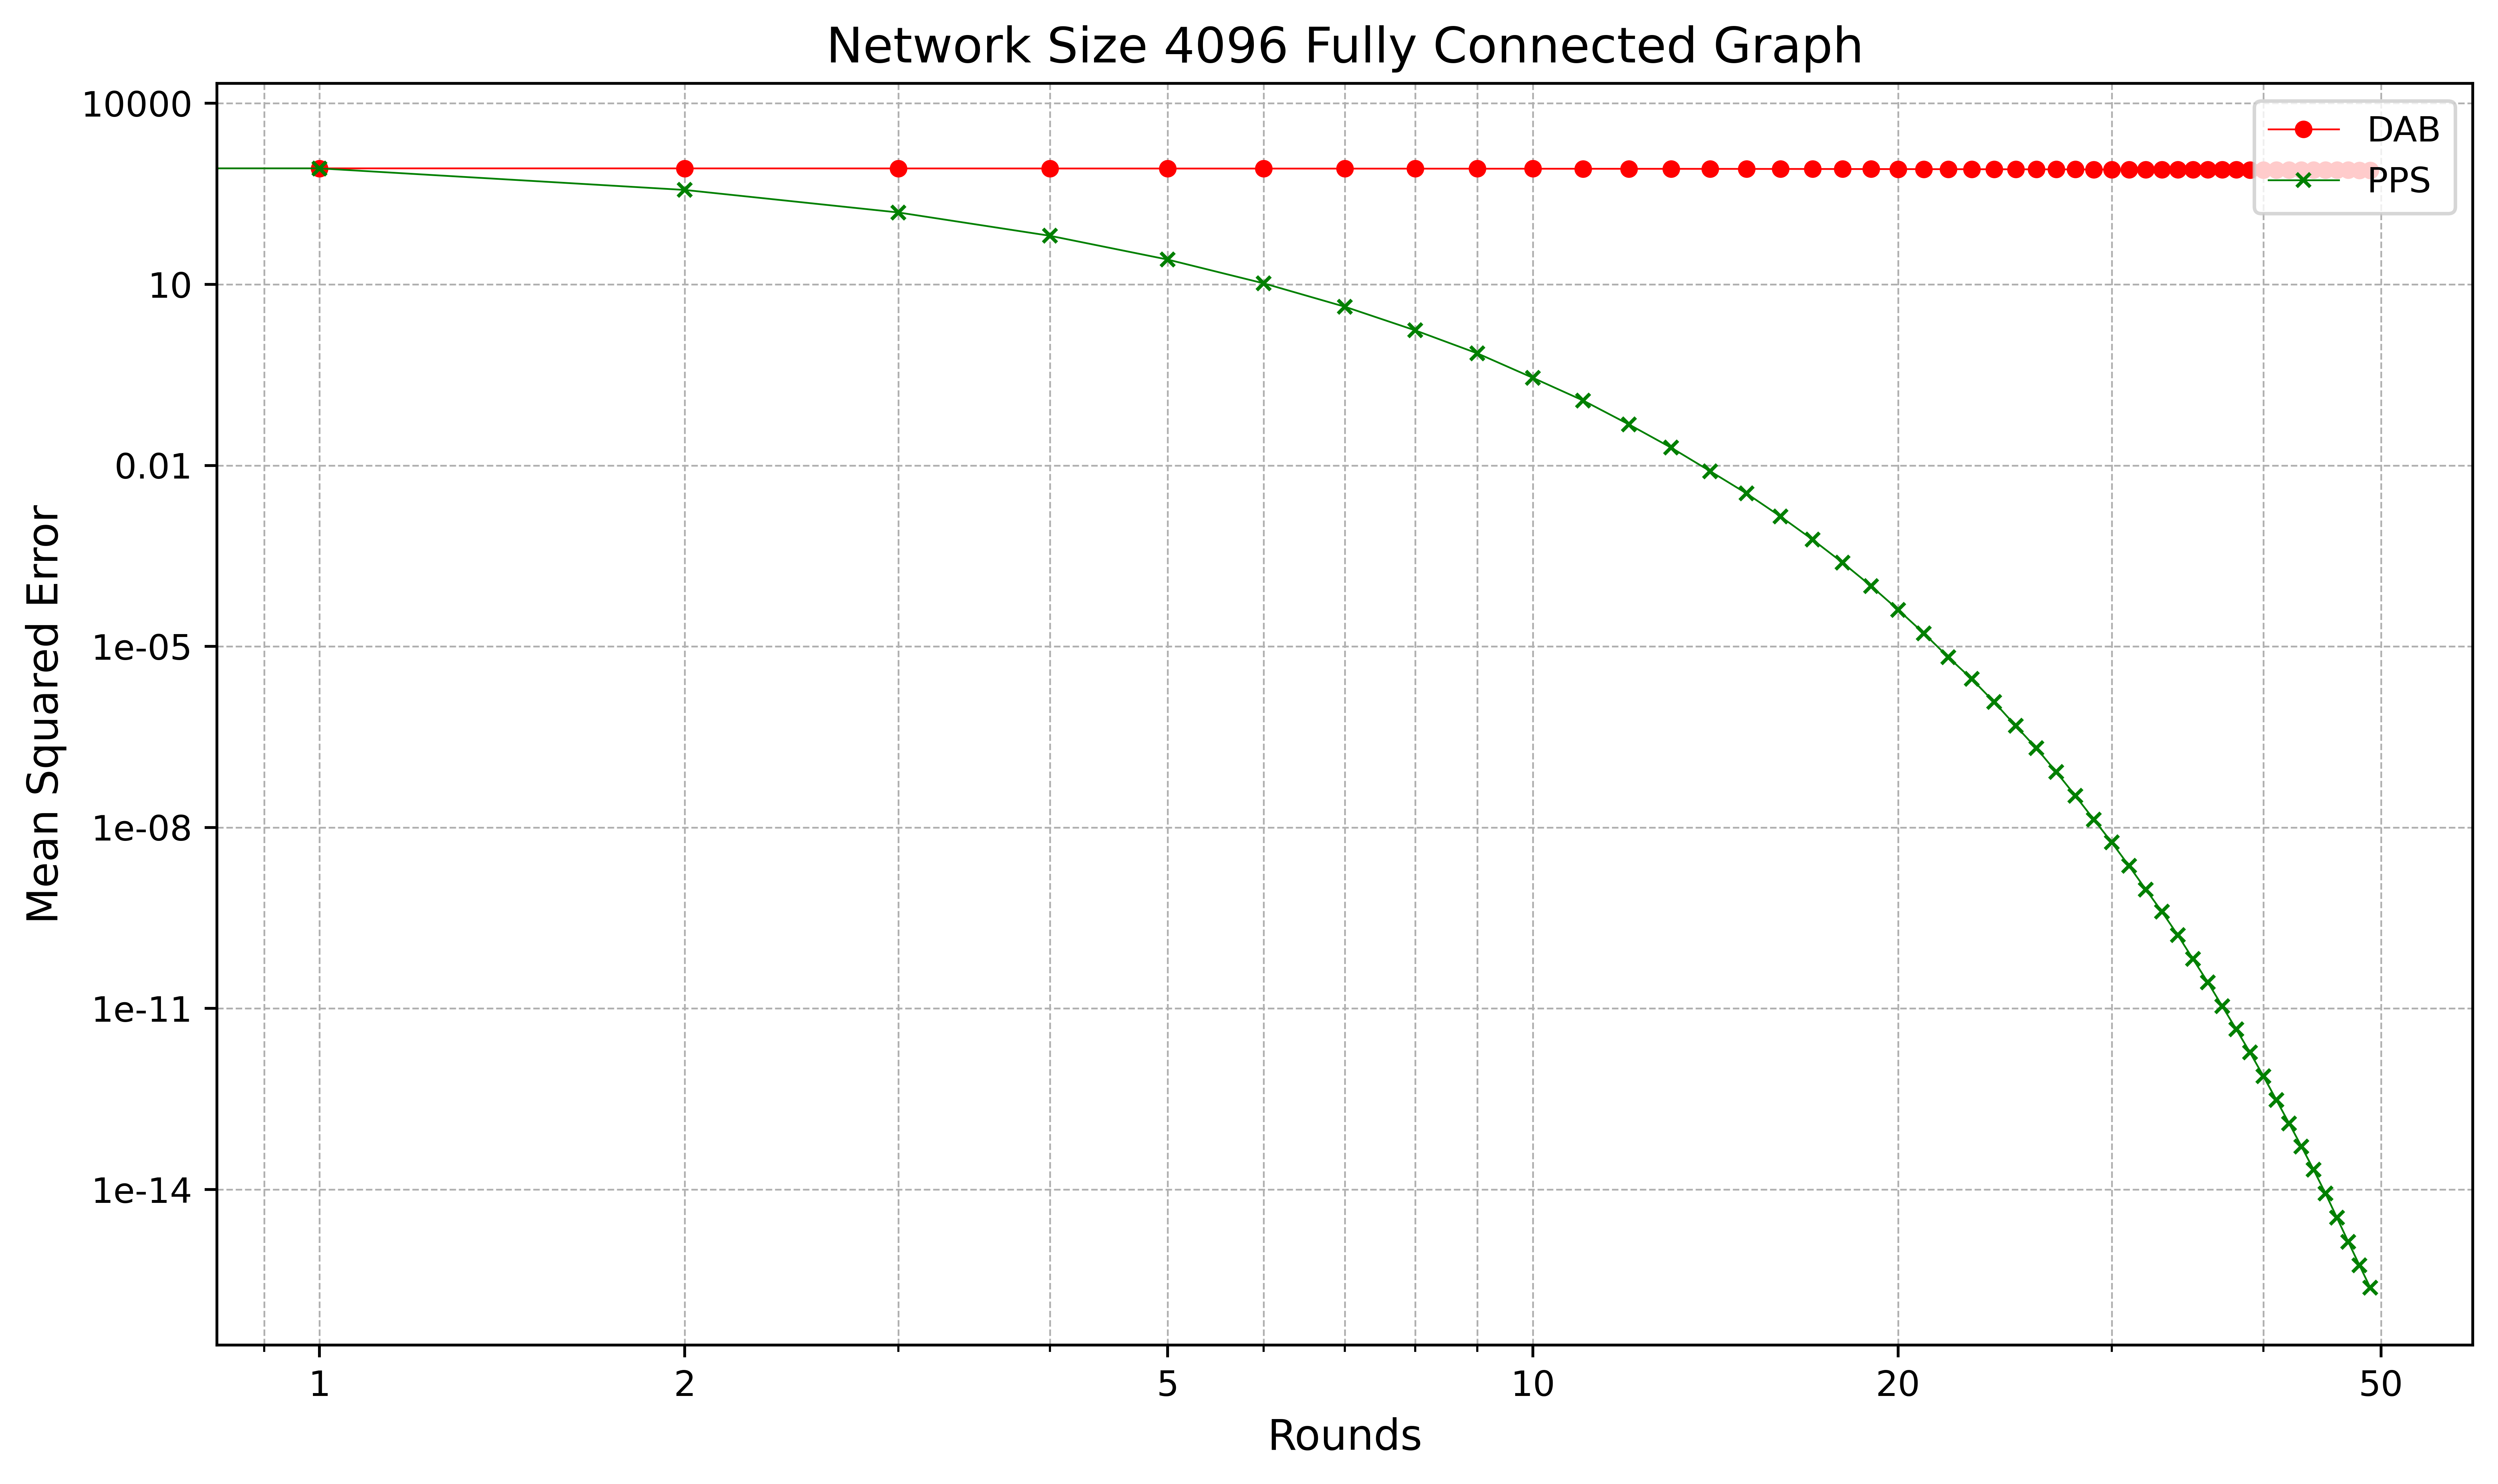
\includegraphics[scale=0.5]{figures/completeGraphSimulations/DAB_vs_PPS_FCG_r50_n4096.png}
    \caption{Fully connected graph: network size $2^{12}$ nodes}
    \label{fig:4096CompleteGraph}
\end{figure}
\begin{figure}[H]
    \centering
    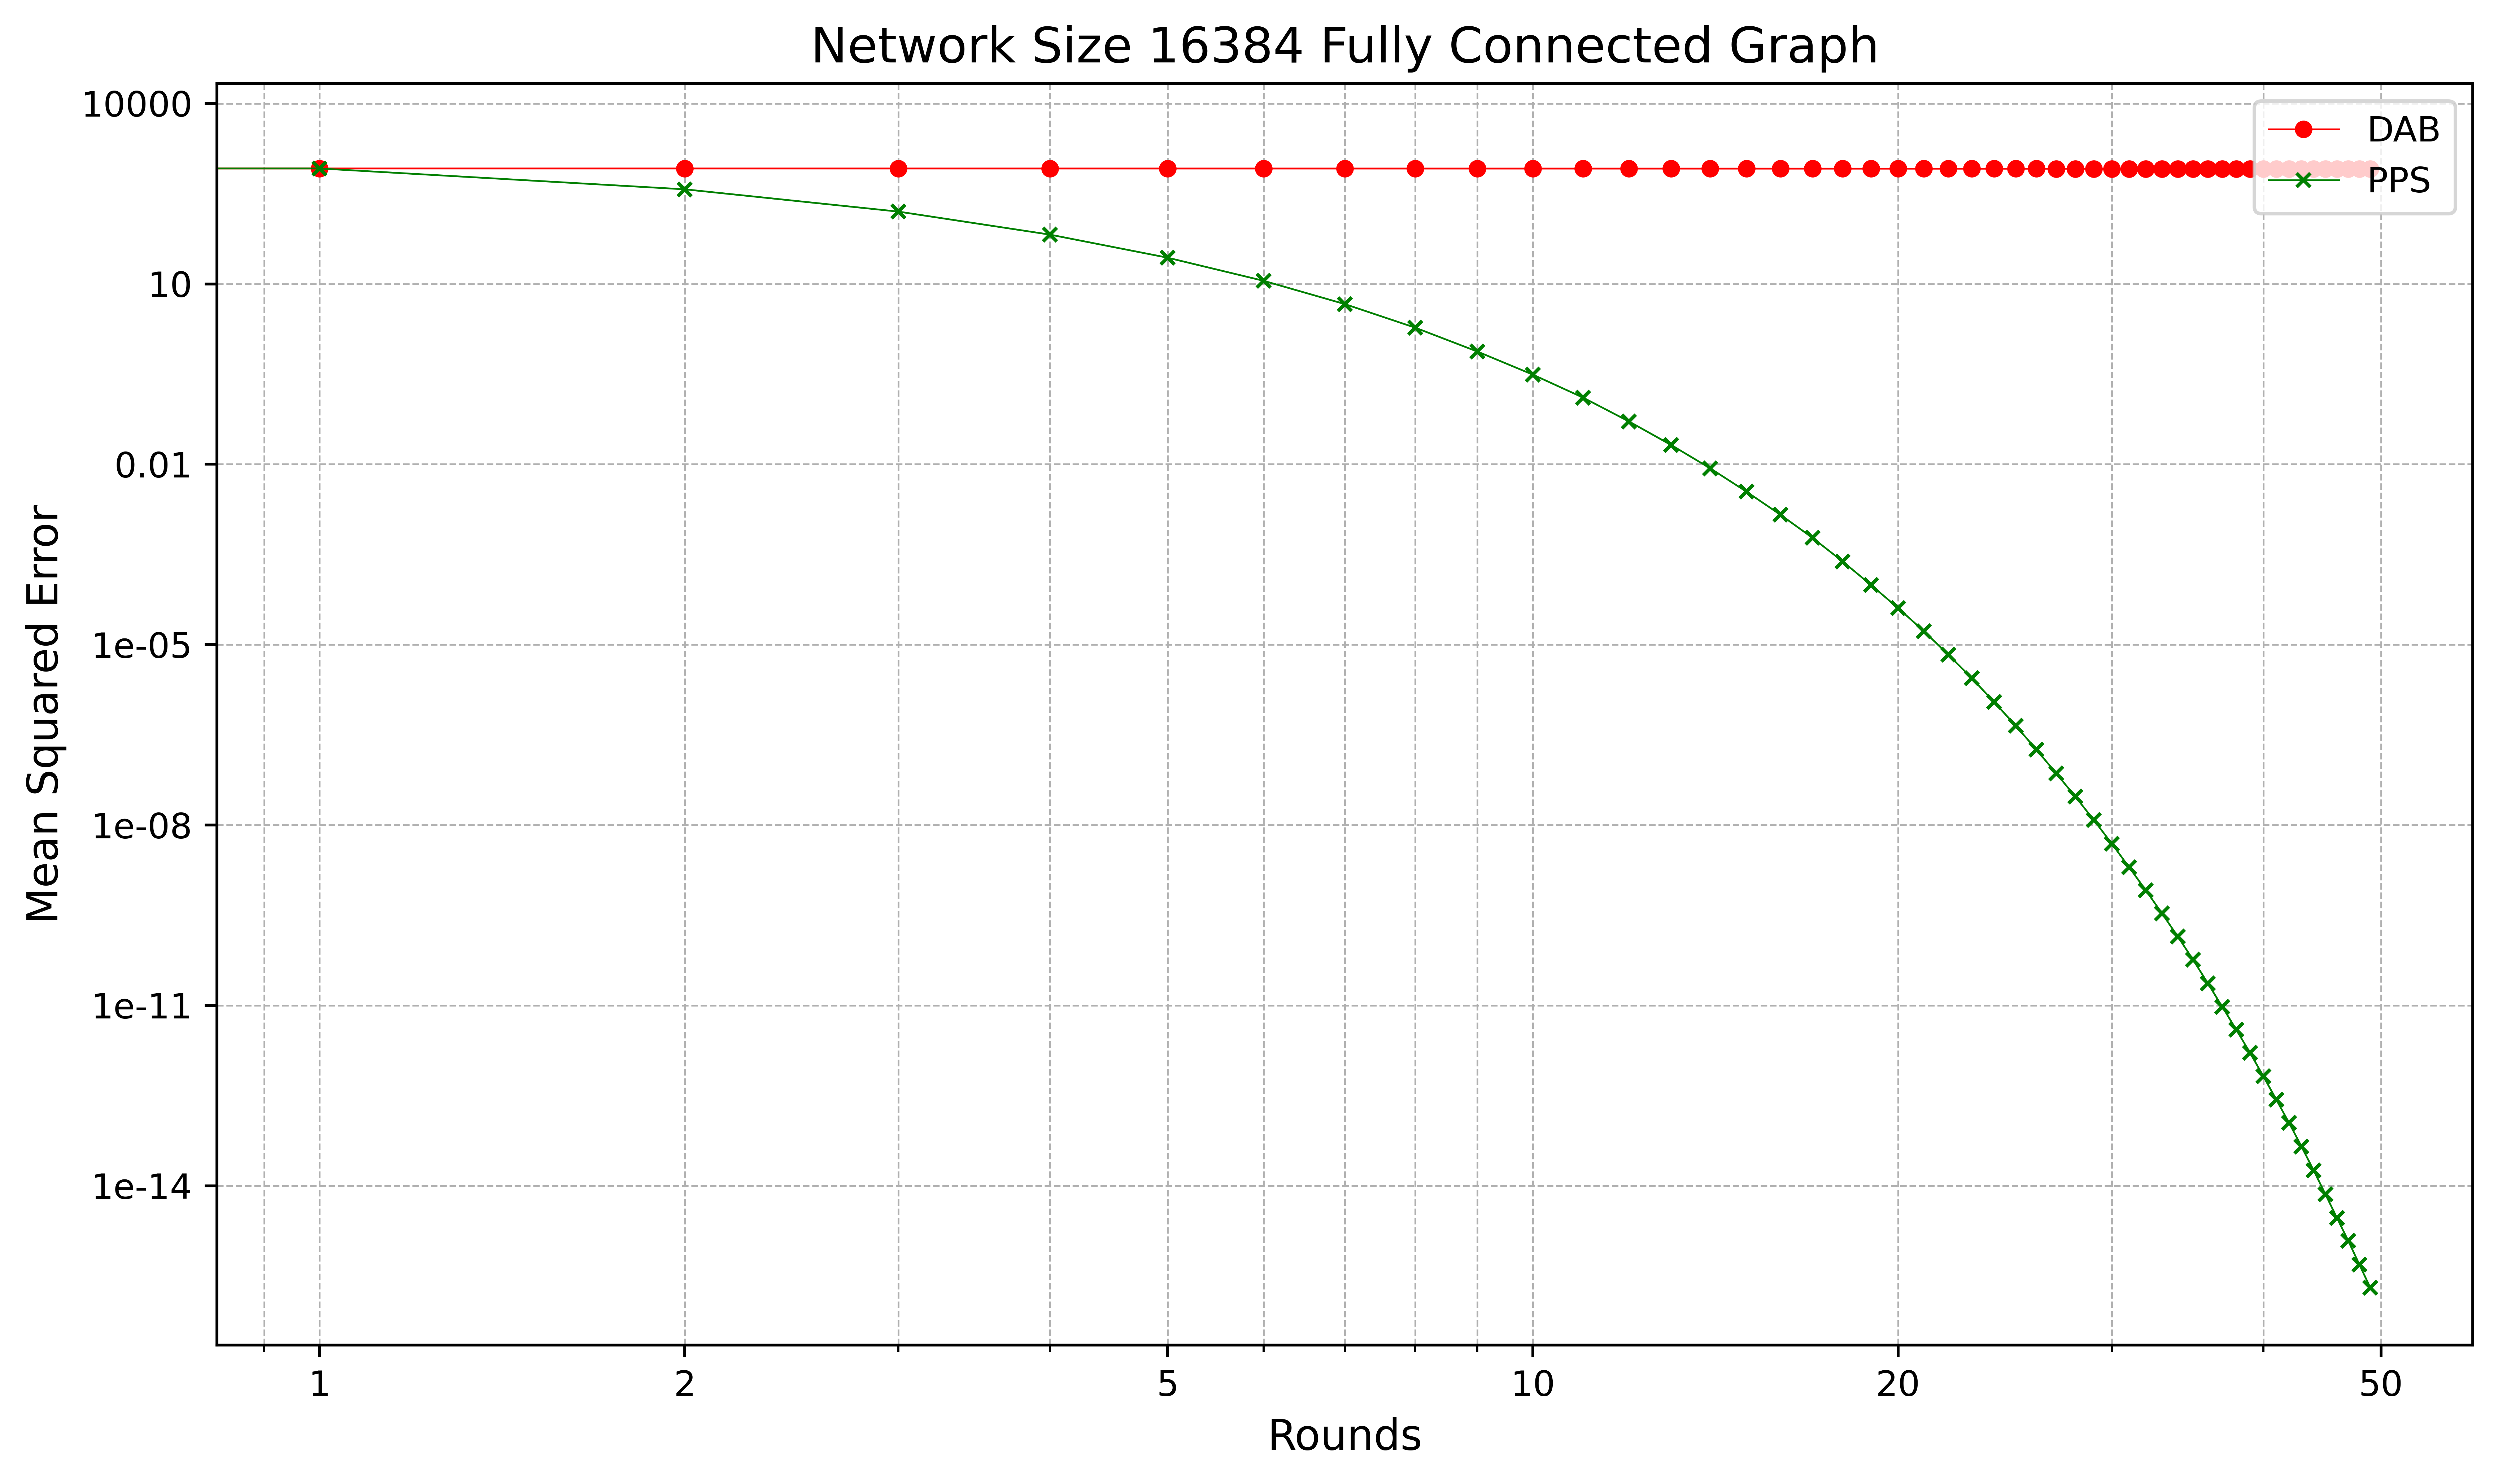
\includegraphics[scale=0.5]{figures/completeGraphSimulations/DAB_vs_PPS_FCG_r50_n16384.png}
    \caption{Fully connected graph: network size $2^{14}$ nodes}
    \label{fig:16384CompleteGraph}
\end{figure}


\section{Star Graph}
\textbf{The star graph}: A star graph as depicted in \hyperref[fig:stargraphDemo]{figure} \ref{fig:stargraphDemo} is a complete bipartite graph \cite{west2001introduction}. A graph is characterized as bipartite graph, if the set of graph edges is the union of two disjoint independent sets \cite{GraphTheorySchindelhaauer2021}. The central node is part of one set, while the remaining outer nodes are part of another set. A star with $n$ nodes has $n-1$ edges. The degree of every node is 1, except for one node, which has the degree of $n-1$. The diameter of a star graph is 2.
\begin{figure}
    \centering
    \begin{tikzpicture}
    \node[draw, fill=blue, circle] (center) at (0, 0) {};
    \foreach \i in {1,...,15} {
            \node[draw, fill=blue, circle] (n\i) at ({360/15 * (\i-1)}:4) {};
            \draw (center) -- (n\i);
        }
\end{tikzpicture}
    \caption{Star graph: network size 16}
    \label{fig:stargraphDemo}
\end{figure}
\subsection{Network Sizes 2\textsuperscript{4}, 2\textsuperscript{8}, 2\textsuperscript{12}, 2\textsuperscript{14}}
\textbf{Analysis}: The PPS algorithm outperforms the DAB in terms of error reducing in every network size we have simulated. For small network sizes, you can at least see a drop in the curve. In the end, however, the network balanced with the DAB algorithm still has an MSE of around 0.001. The network balanced with the PPS algorithm has already reached an MSE of $1e-23$ and is therefore far more balanced. For larger network sizes, there is no longer a straight line for the DAB balanced network. Instead, a stagnating graph can be observed. A look at the simulation outputs shows: For the three network sizes $2^{8}$, $2^{12}$ and $2^{14}$, the MSE in the 50th round for the DAB balanced network is around 100. meanwhile, the MSE of the PPS balanced network is $<1e-20$, and therefore far better. This is due to the characteristic structure of the star graph. The star graph is a complete bipartite graph, with only the central node in one set and all other nodes in the other set. Each outer node is only connected to the inner node. For the DAB, this means that when searching for the minimum node, only the inner node comes into question. However, if the inner node has a higher load than the outer node, a load transfer is already ruled out. This behaviour means that the network error is reduced very slowly. The PPS, on the other hand, benefits from such a structure. Each node selects the inner node as a trading partner. This means that every node is also involved in a load transfer per round. Each push action of the outer node is followed by a pull action of the inner node. What is now observable, however, is that the inner node is involved in all load transfers. This node therefore fulfils a large part of the balancing procedure. This can lead to problems to the extent that a load transfer is not exactly a cheap operation. If a node is involved in every load transfer, this means a very one-sided load on a node. For the DAB in the star graph scenario there is also a one-sided loading of a node, however with much less load transfers per round. Another observation that emerges from the graph is that the PPS algorithm does not have the ‘anytime’ property. In rounds 47-50, there is a short-term increase in the error for the three network sizes $2^{8}$, $2^{12}$ and $2^{14}$. Such behaviour is not observed for the DAB algorithm.\\
\textbf{Winner}: PPS
\begin{figure}[H]
    \centering
    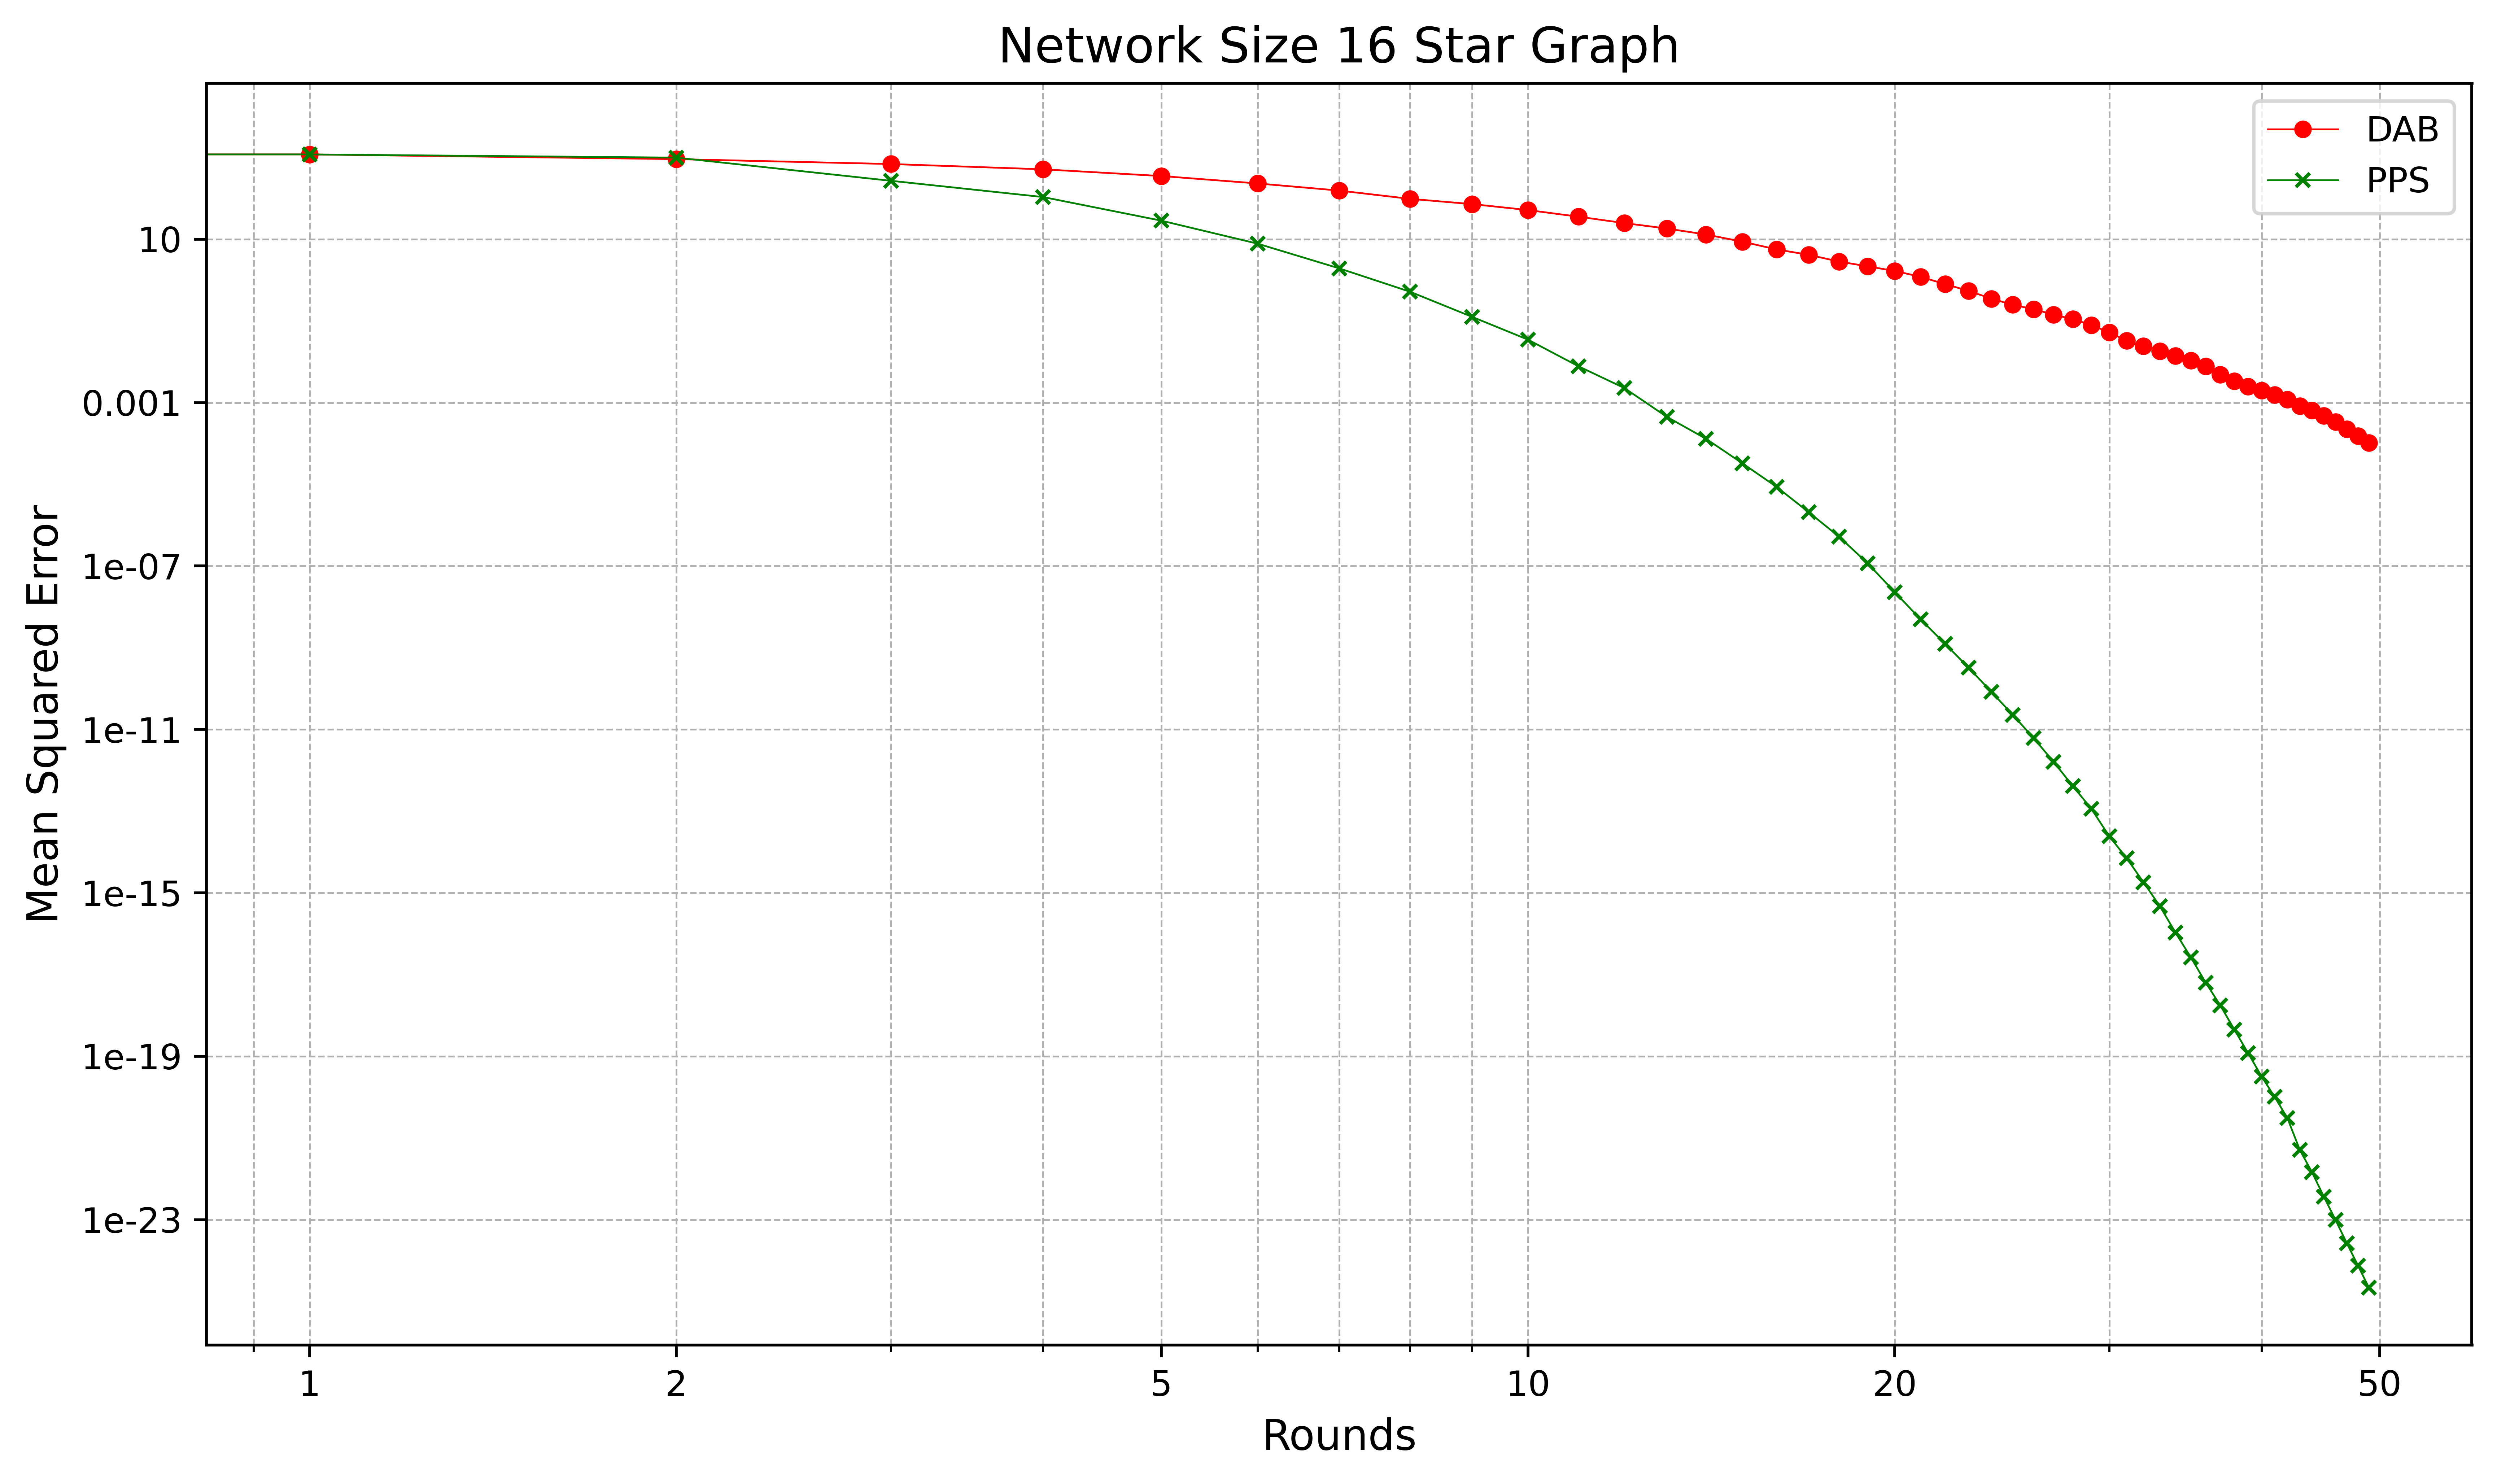
\includegraphics[scale=0.5]{figures/starGraphSimulations/DAB_vs_PPS_SG_r50_n16.png}
    \caption{Star graph: network size $2^{4}$ nodes}
    \label{fig:16StarGraph}
\end{figure}

\begin{figure}[H]
    \centering
    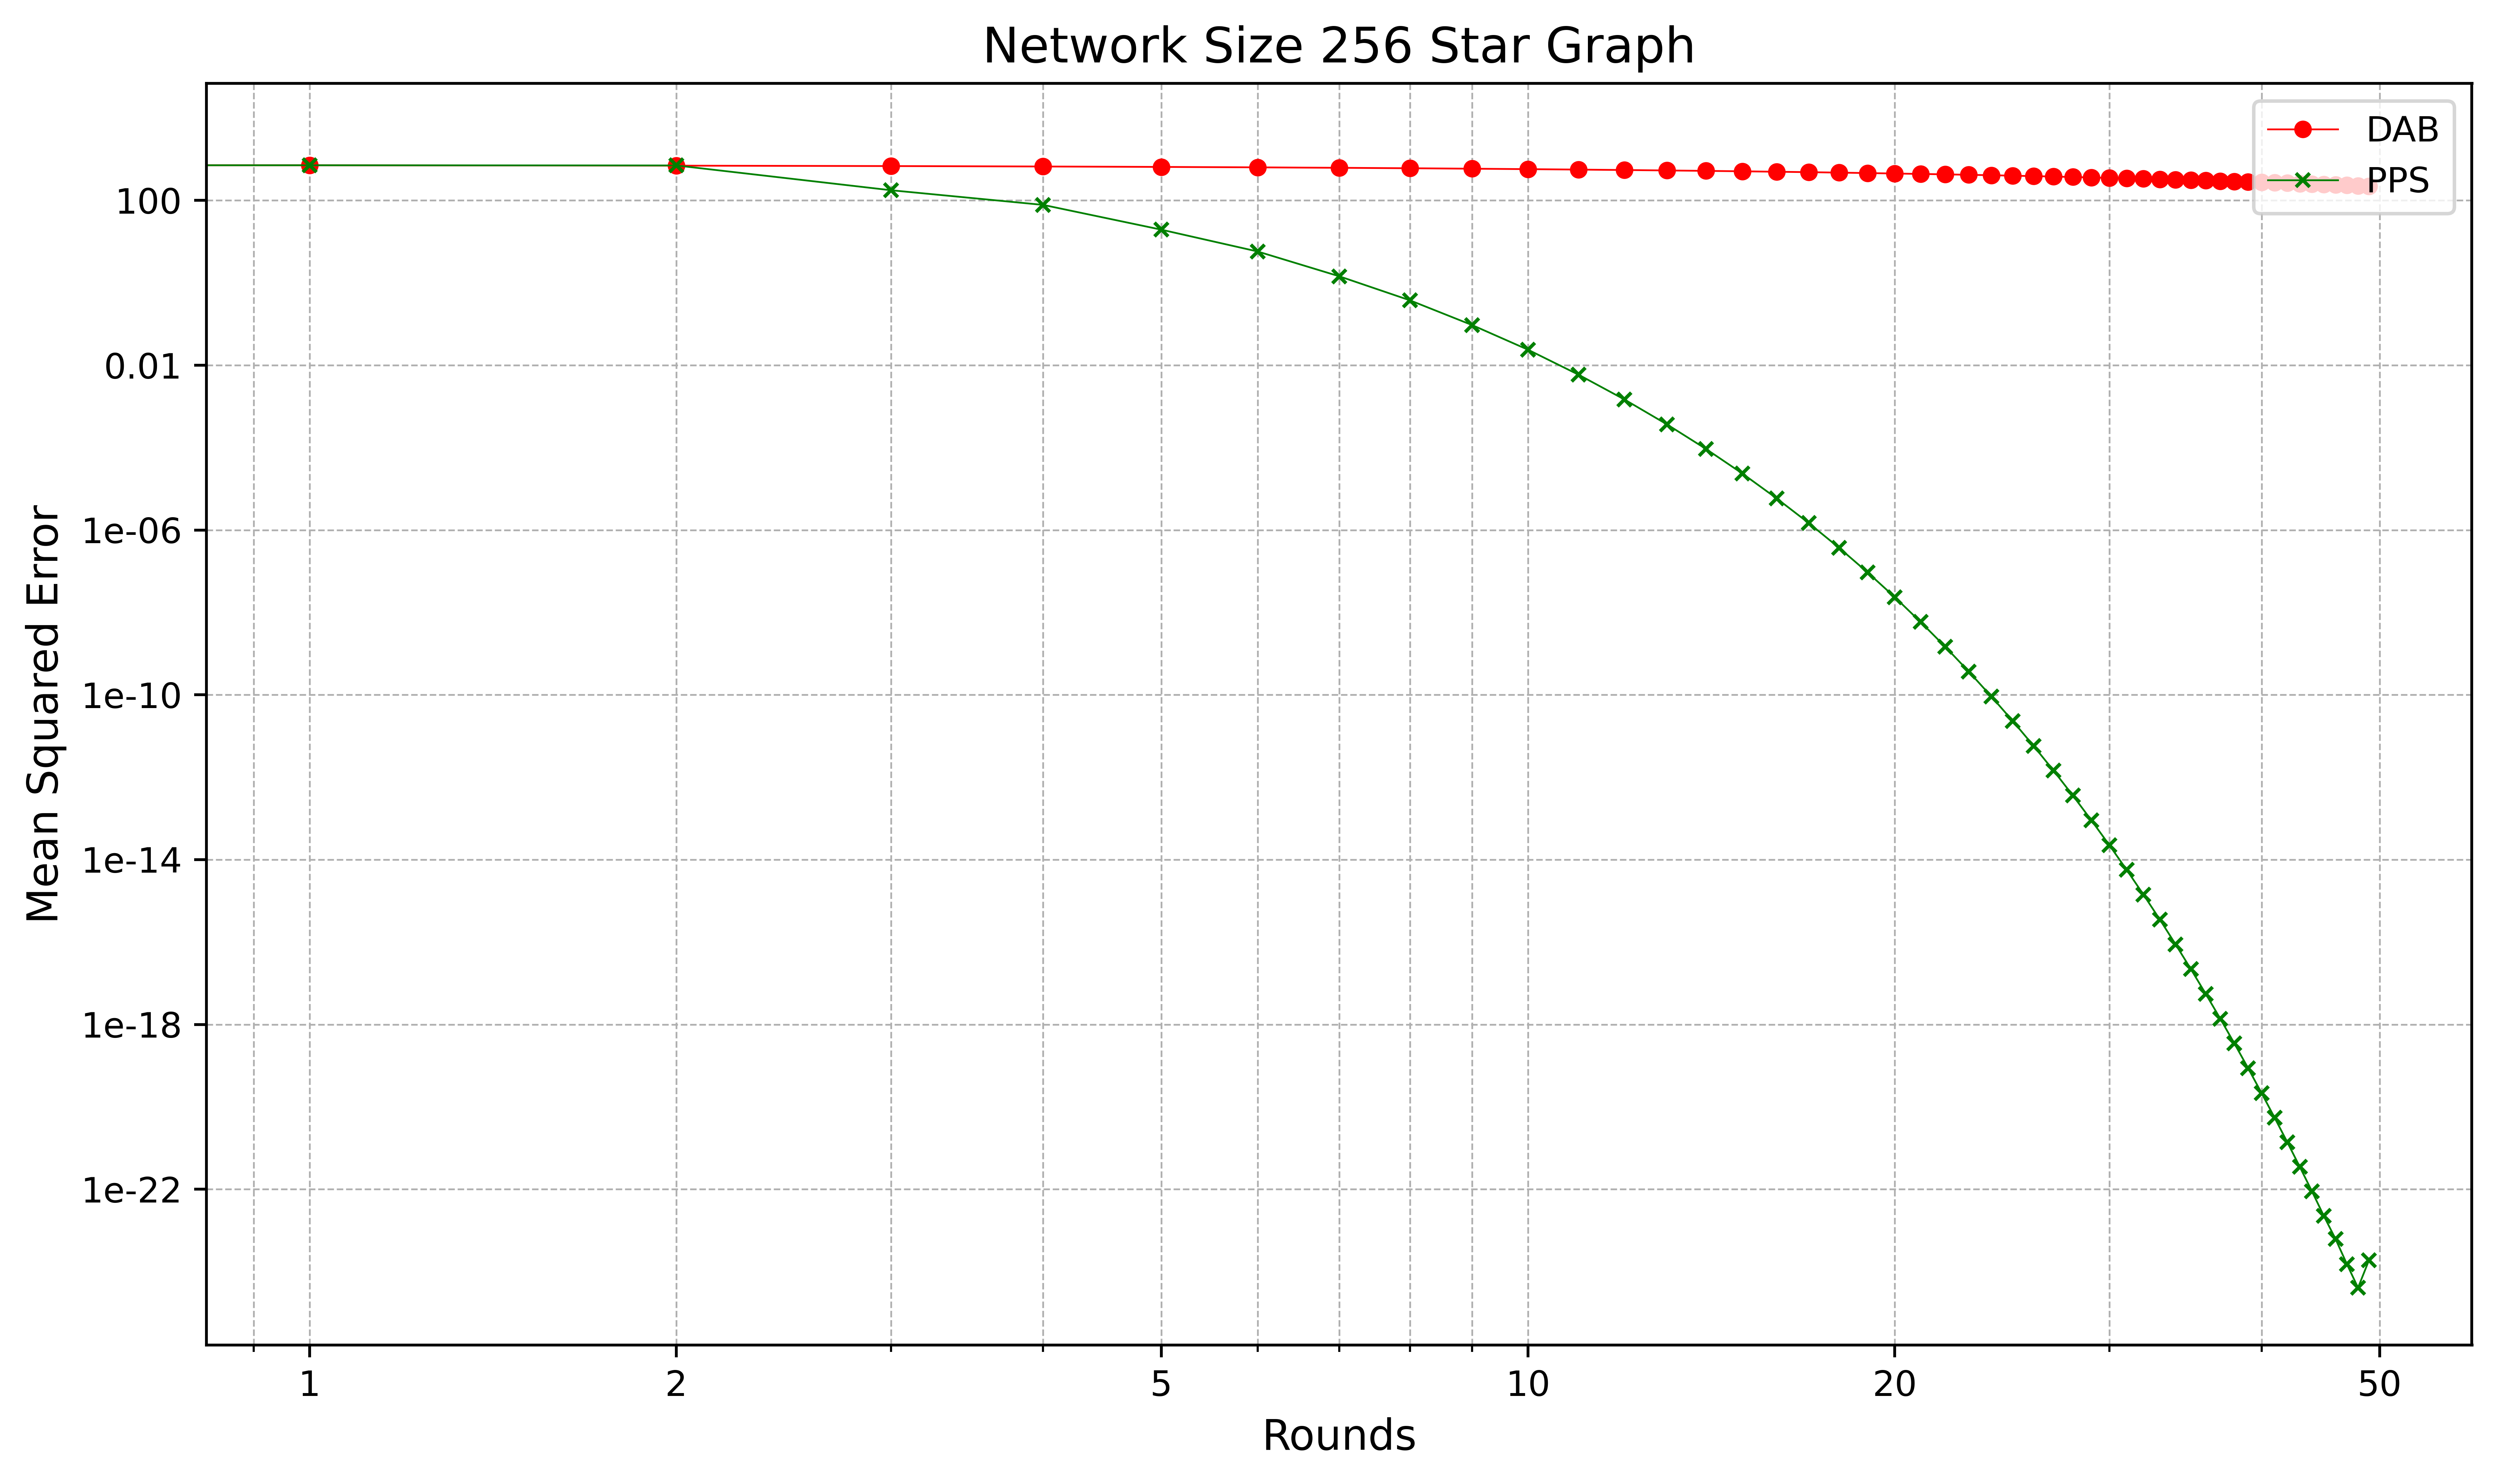
\includegraphics[scale=0.5]{figures/starGraphSimulations/DAB_vs_PPS_SG_r50_n256.png}
    \caption{Star graph: network size $2^{8}$ nodes}
    \label{fig:256StarGraph}
\end{figure}

\begin{figure}[H]
    \centering
    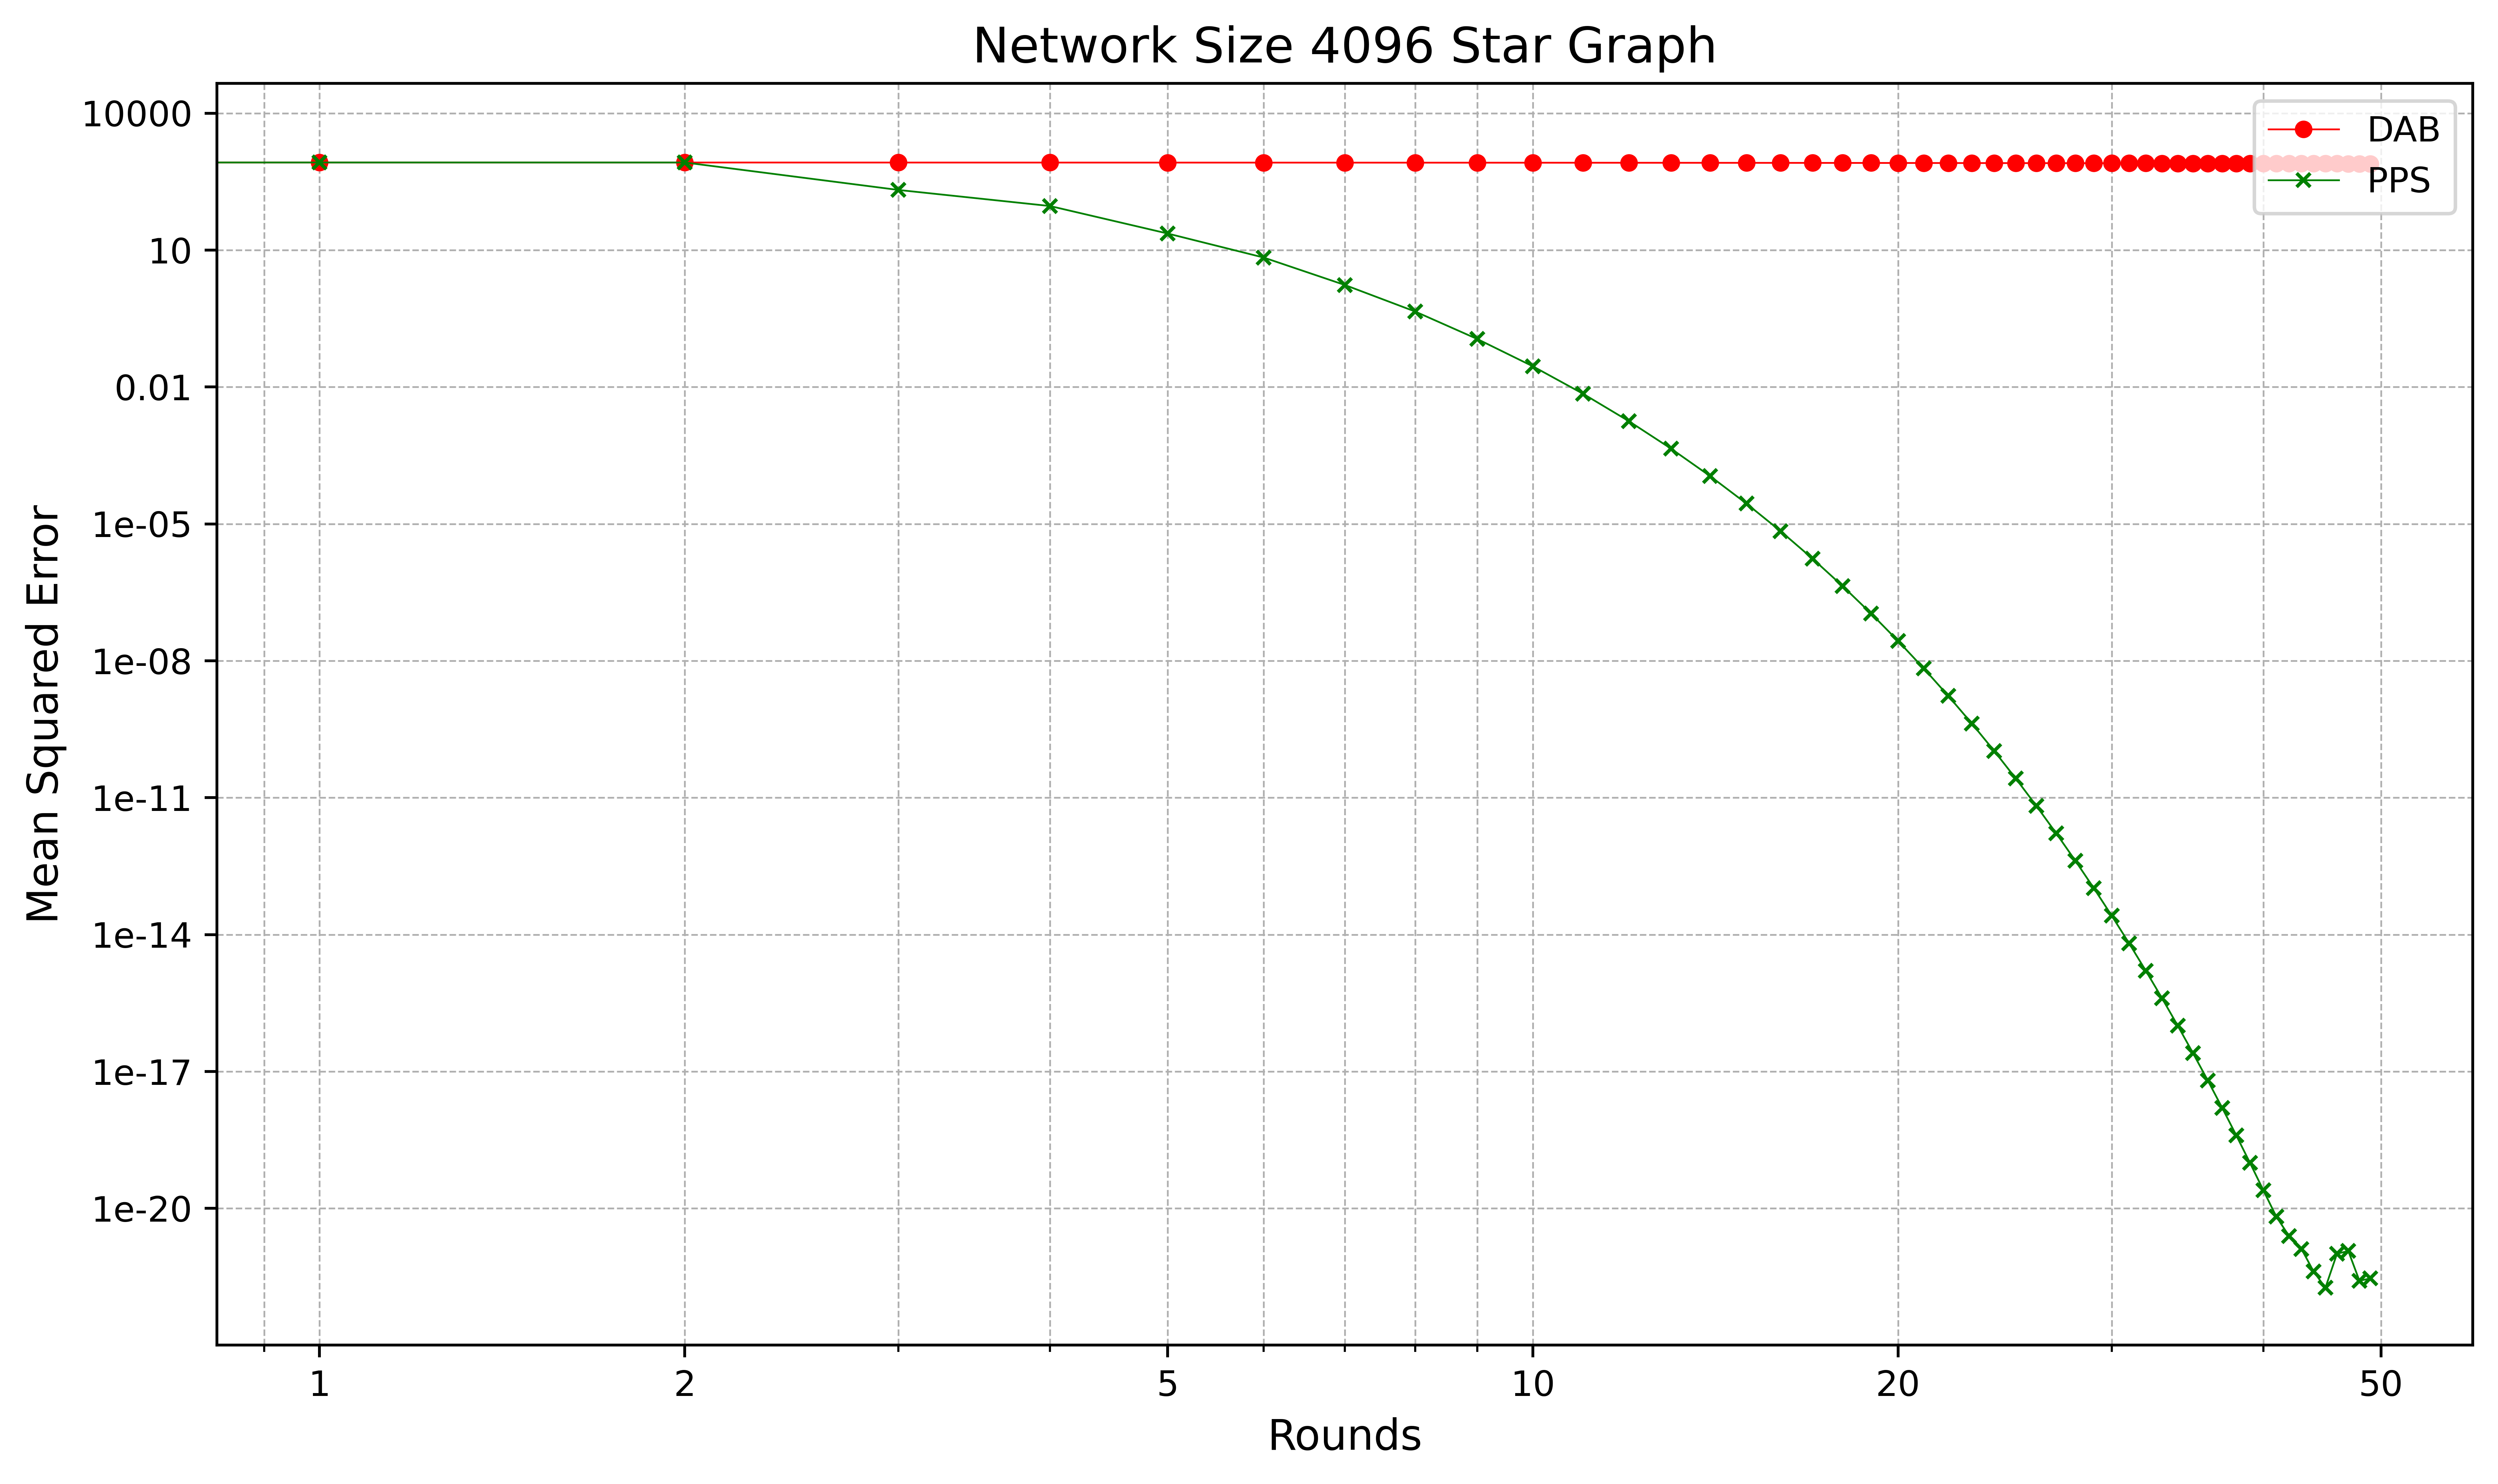
\includegraphics[scale=0.5]{figures/starGraphSimulations/DAB_vs_PPS_SG_r50_n4096.png}
    \caption{Star graph: network size $2^{12}$ nodes}
    \label{fig:4096StarGraph}
\end{figure}

\begin{figure}[H]
    \centering
    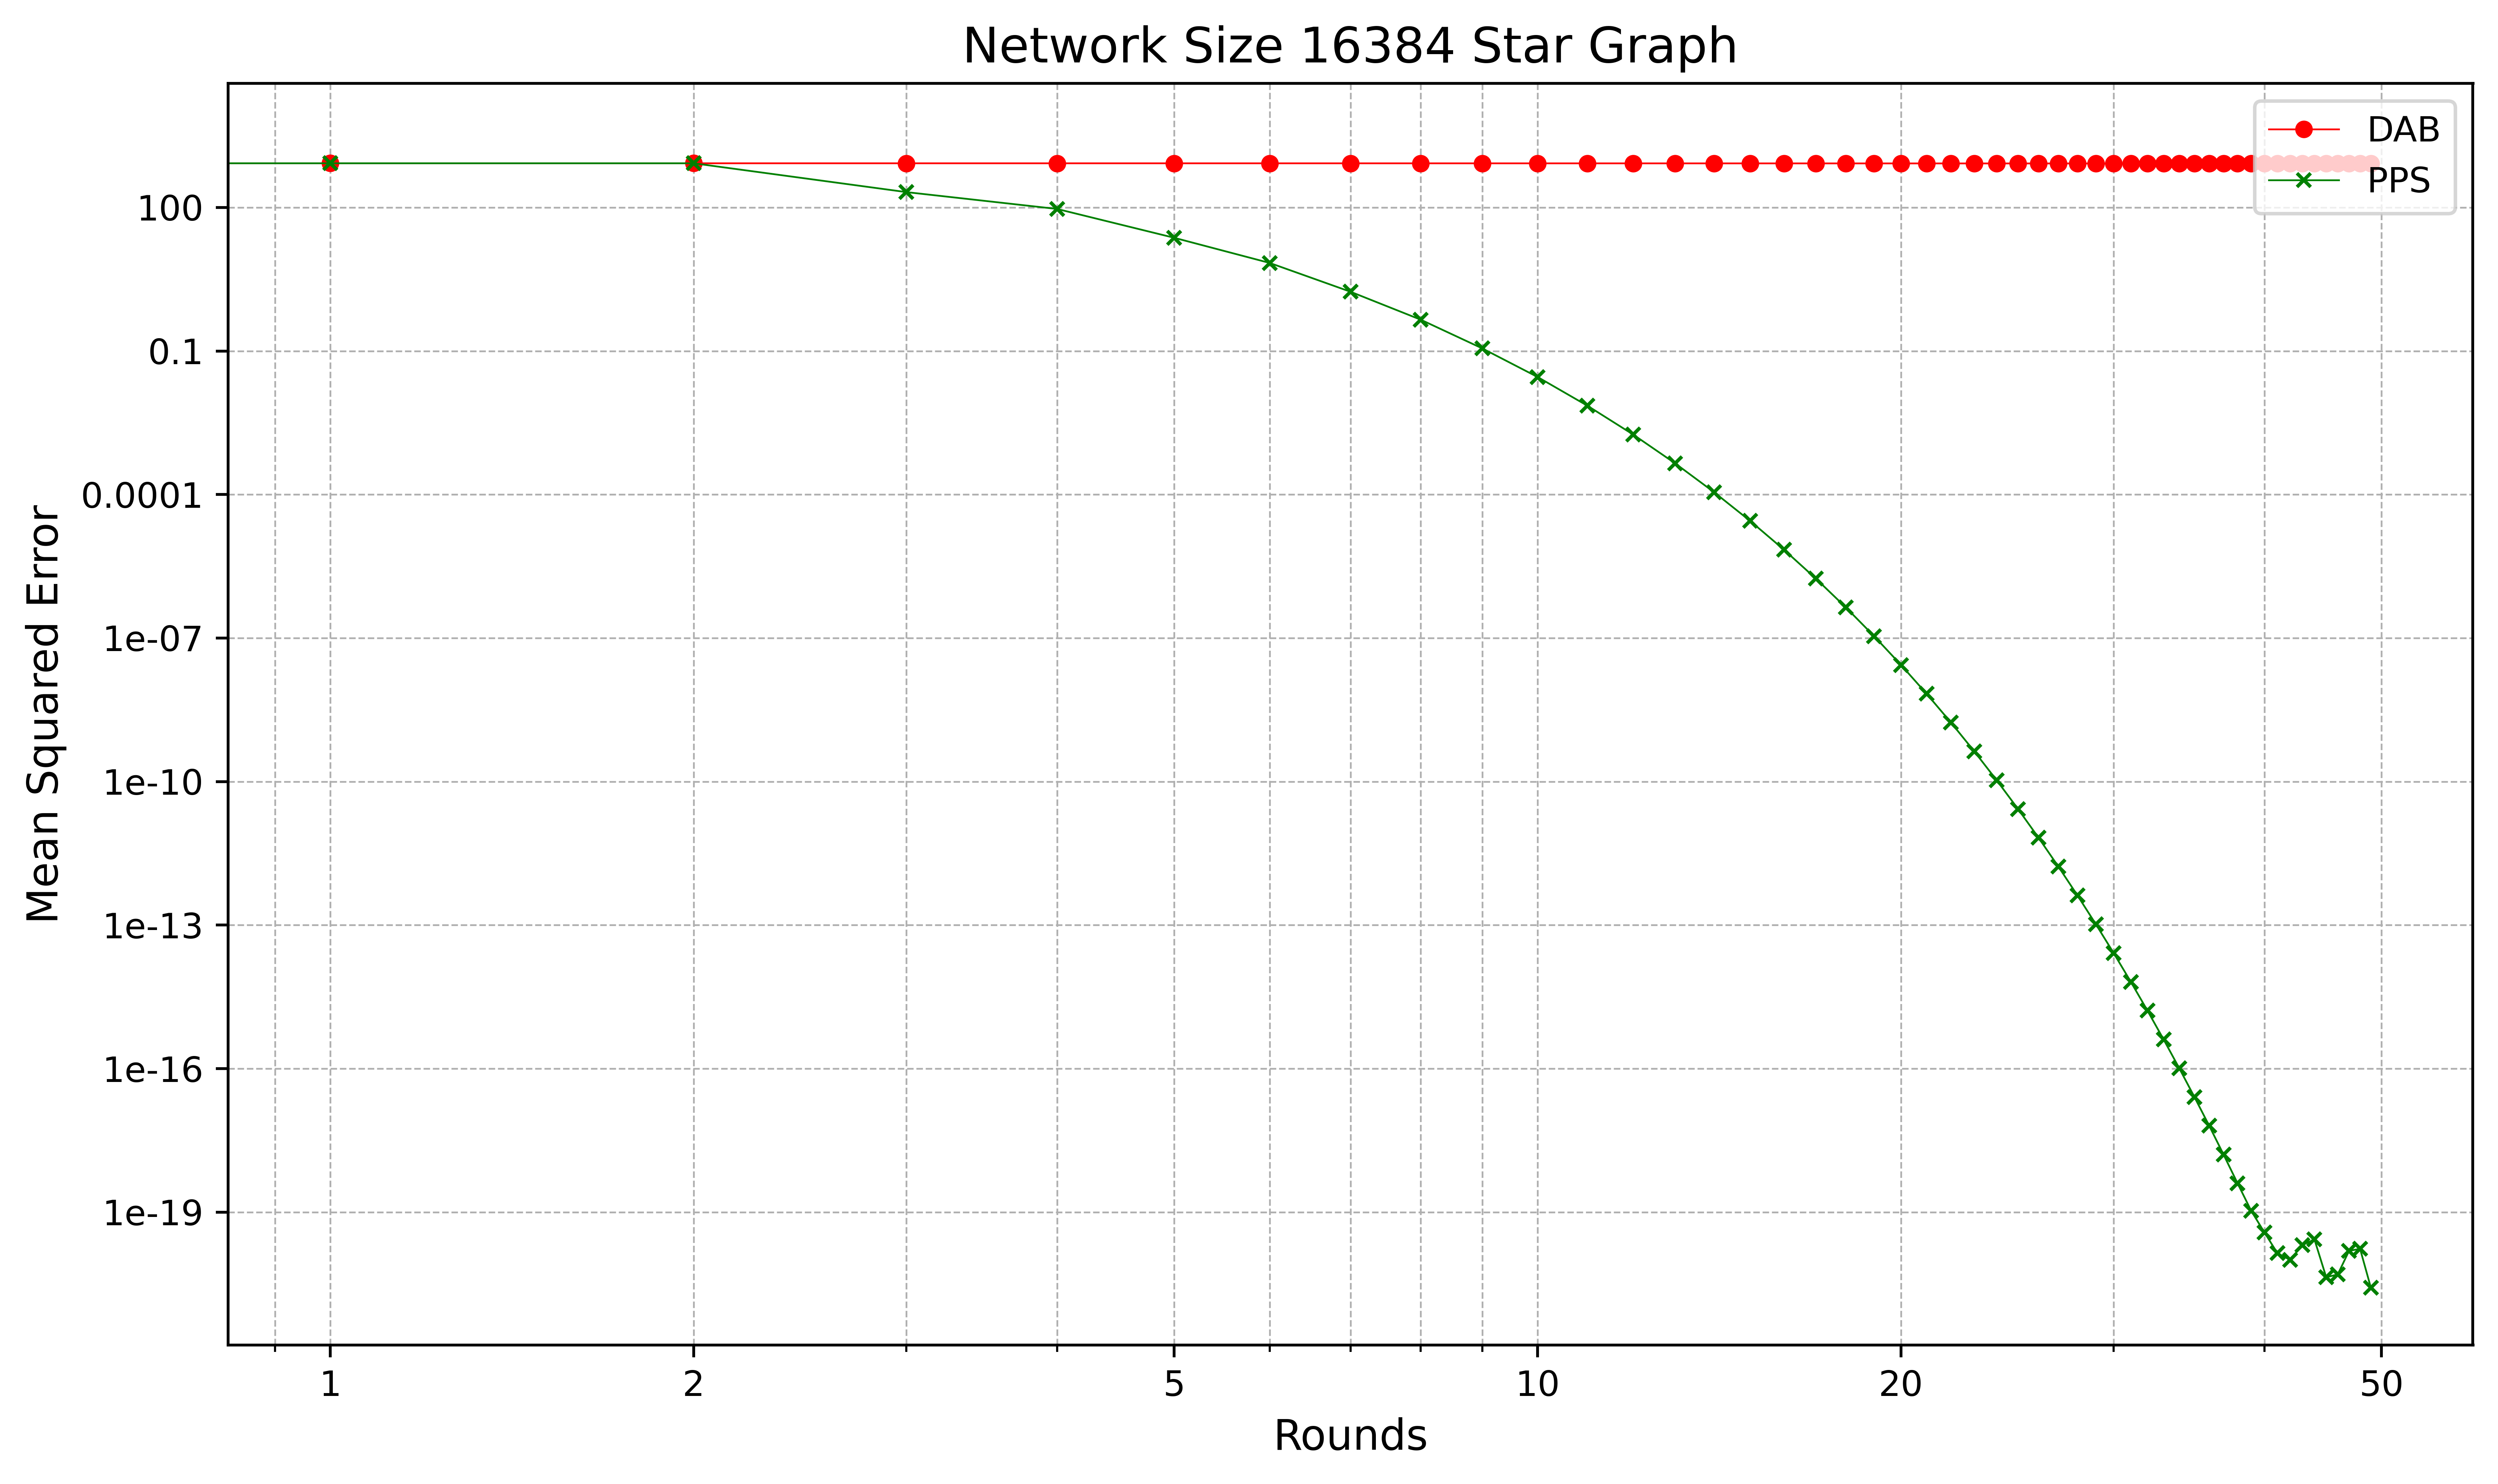
\includegraphics[scale=0.5]{figures/starGraphSimulations/DAB_vs_PPS_SG_r50_n16384.png}
    \caption{Star graph: network size $2^{14}$ nodes}
    \label{fig:16384StarGraph}
\end{figure}

\section{Closed Chain Graph}
\textbf{The closed chain graph}: A closed chain graph (or also refered to as closed path graph) is a regular graph where each node has a degree of two. A chain graph can be drawn so that all of its vertices and edges lie on a single straight line \cite{gross1998graph}. For a closed chain graph, the first and the last node are also connected as depicted in \hyperref[fig:closedChainGraphDemo]{figure } \ref{fig:closedChainGraphDemo}. Furthermore, a closed chain graph has $n$ edges.
\begin{figure}
    \centering
    \scalebox{0.8}{\begin{tikzpicture}
    \foreach \i in {1,...,16} {
      \node[draw, fill=blue, circle, minimum size=6pt] (v\i) at (\i, 0) {};
    }
    
    \foreach \i in {1,...,15} {
      \pgfmathtruncatemacro{\j}{\i+1}
      \draw (v\i) -- (v\j);
    }
    
    \draw[bend left=45] (v1) to (v16);
  
  \end{tikzpicture}}
    \caption{Closed chain graph: network size 16}
    \label{fig:closedChainGraphDemo}
\end{figure}
\subsection{Network sizes 2\textsuperscript{4}, 2\textsuperscript{8}, 2\textsuperscript{12} and 2\textsuperscript{14}}
\textbf{Analysis}:  \\
\textbf{Winner}: DAB\\
\begin{figure}[H]
    \centering
    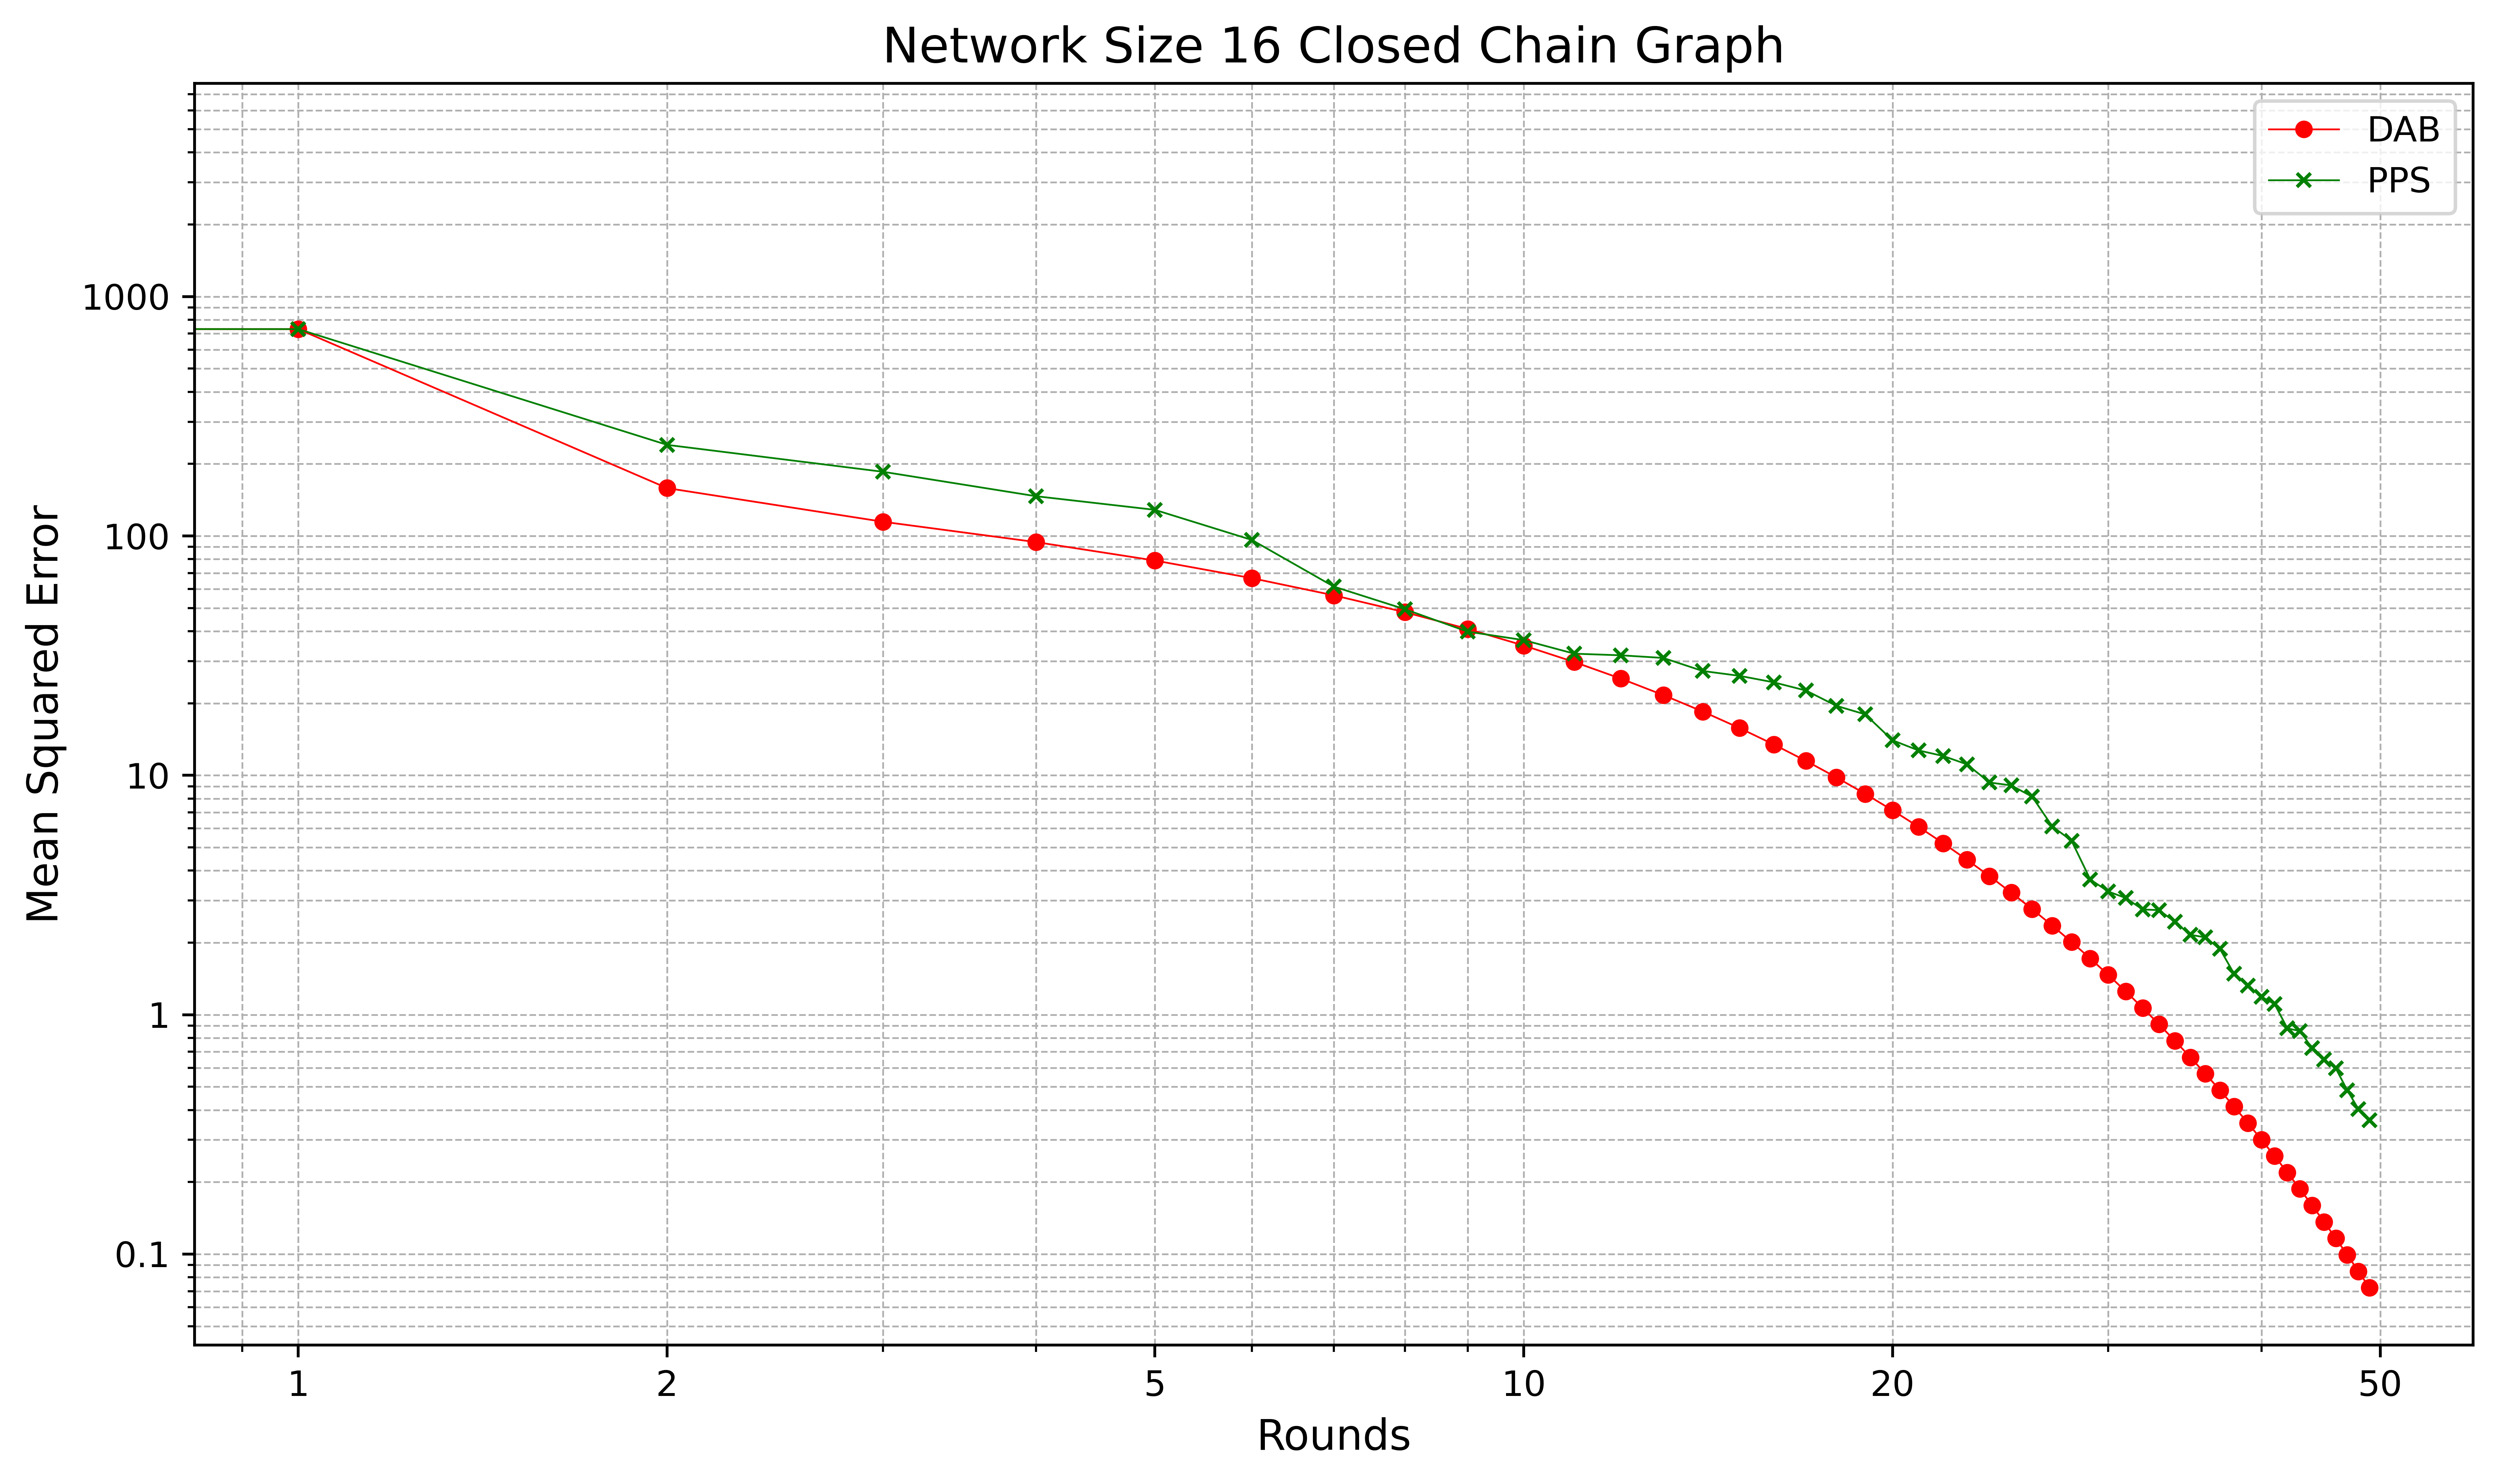
\includegraphics[scale=0.5]{figures/closedChainSimulations/DAB_vs_PPS_CCG_r50_n16.png}
    \caption{Closed chain graph: network size $2^{4}$ nodes}
    \label{fig:16ChainGraph}
\end{figure}

\begin{figure}[H]
    \centering
    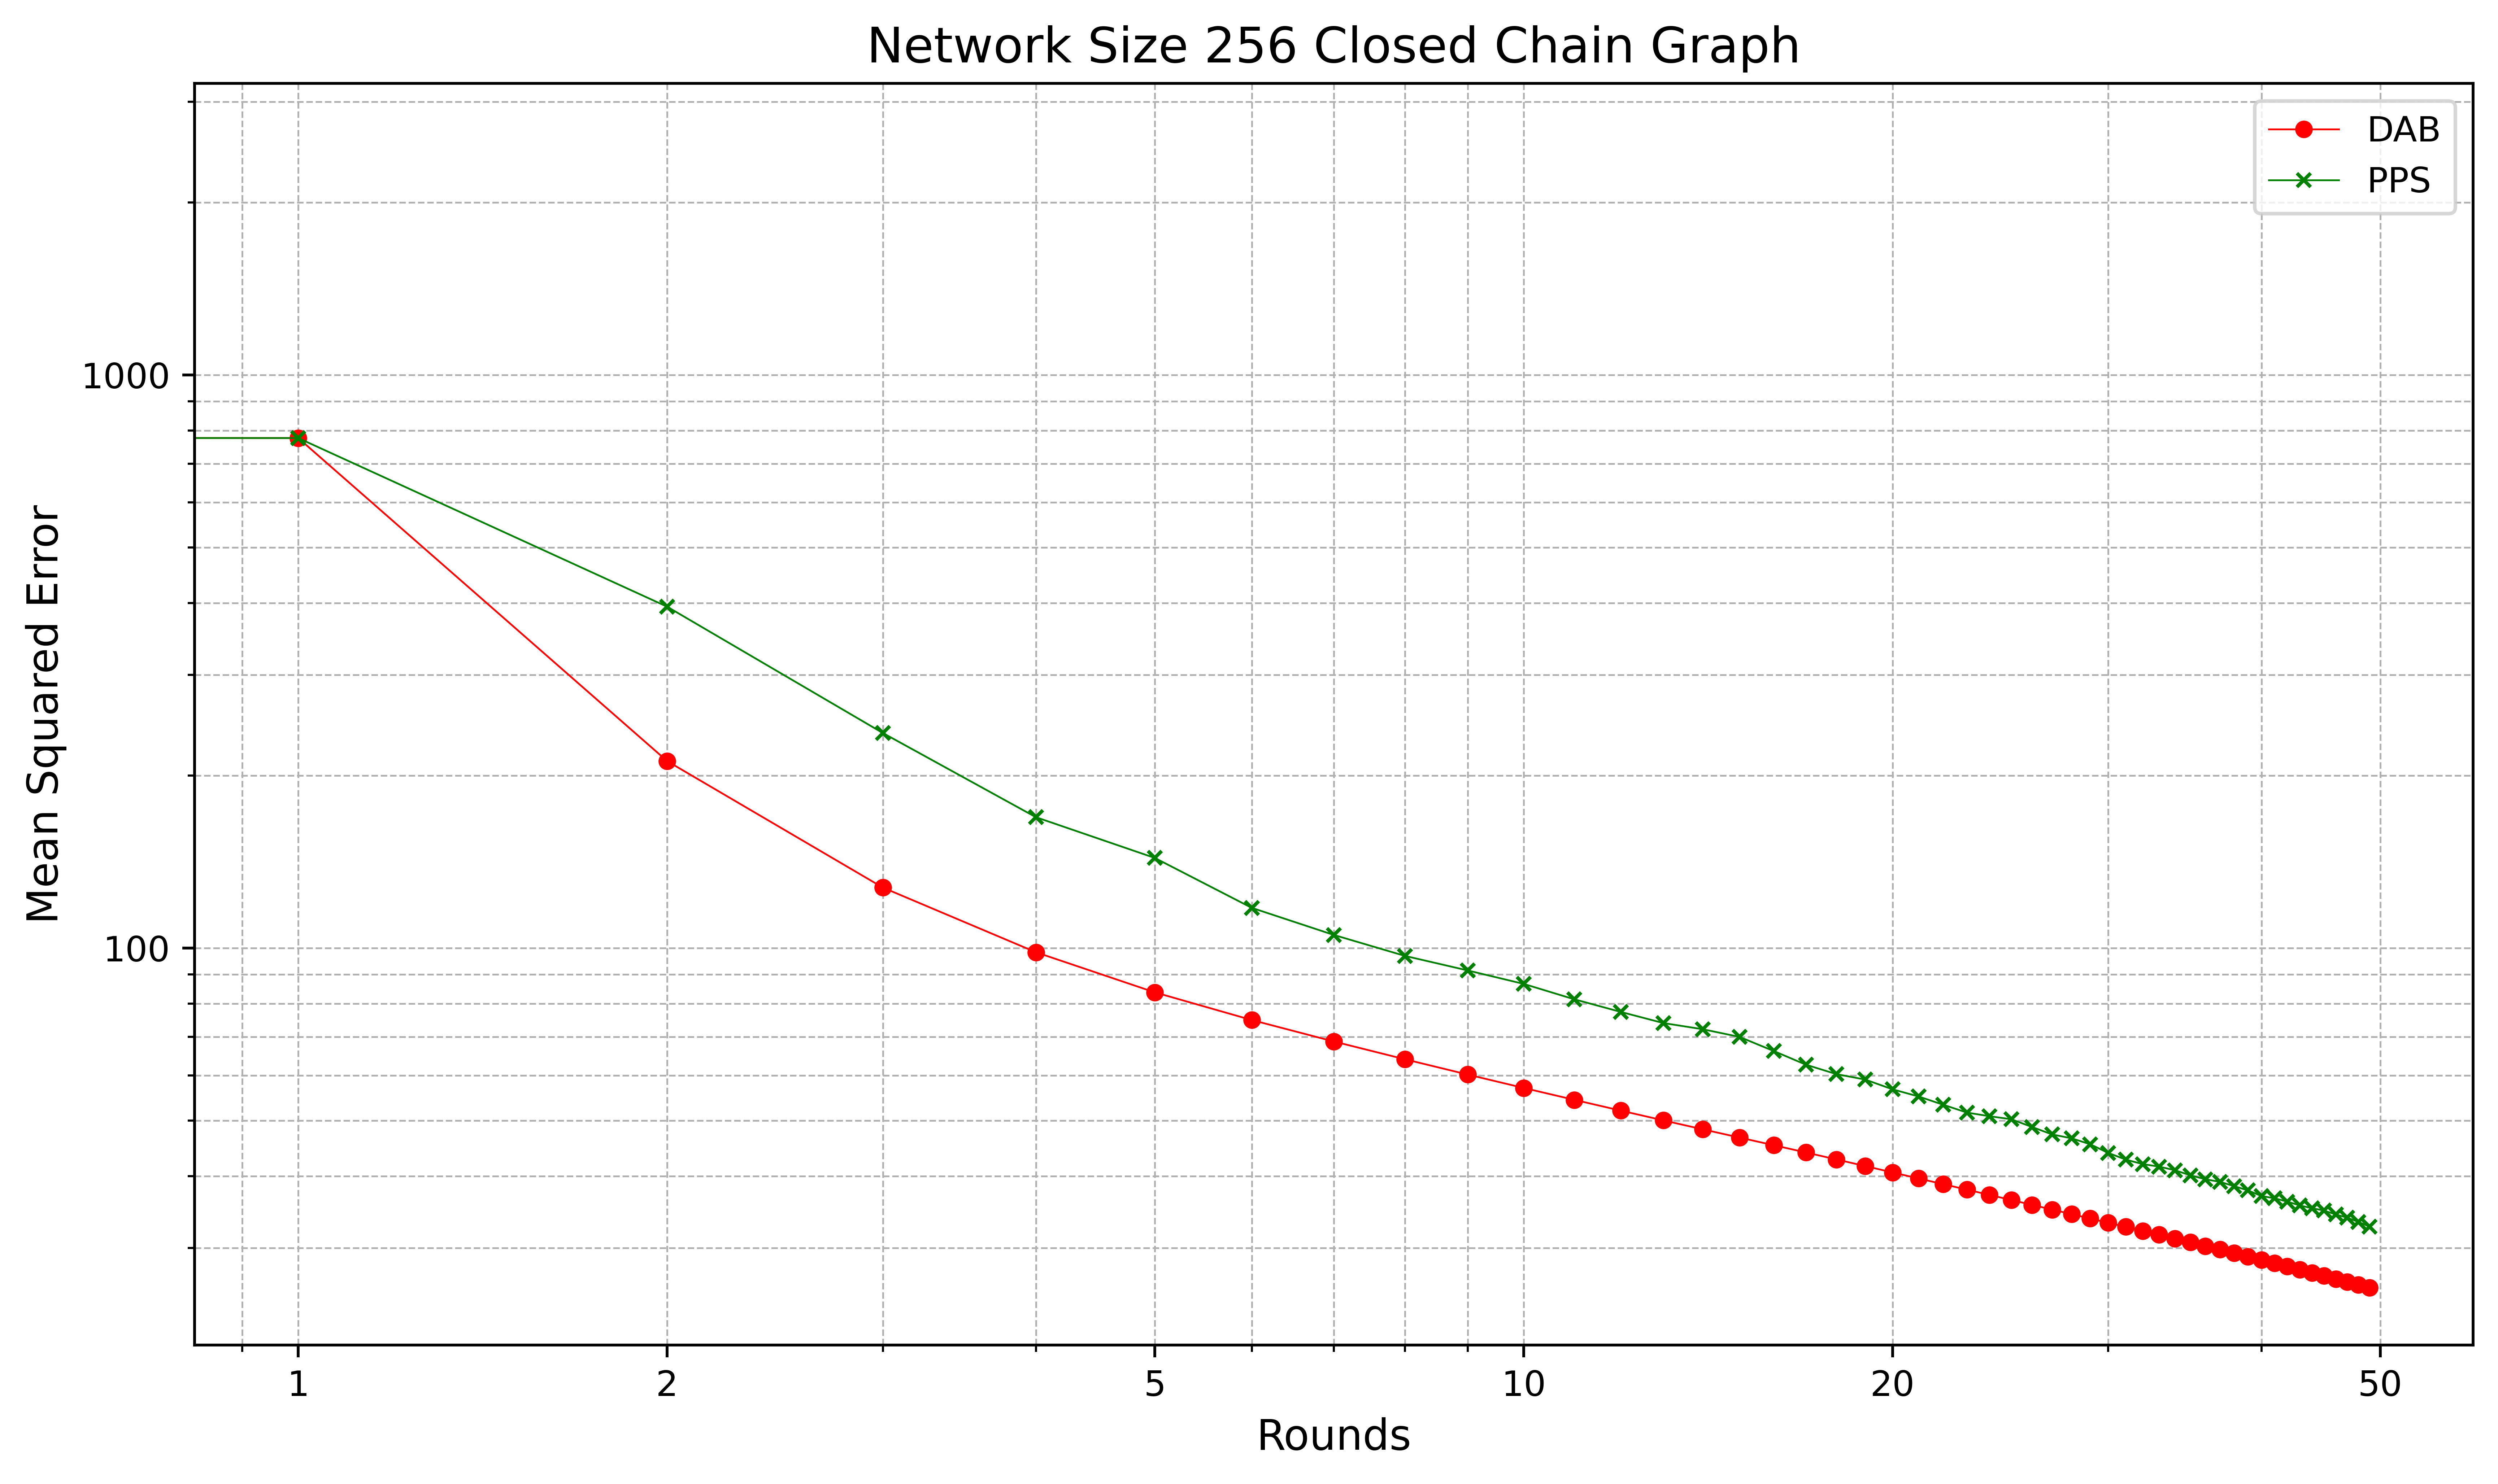
\includegraphics[scale=0.5]{figures/closedChainSimulations/DAB_vs_PPS_CCG_r50_n256.png}
    \caption{Closed chain graph: network size $2^{8}$ nodes}
    \label{fig:256ChainGraph}
\end{figure}

\begin{figure}[H]
    \centering
    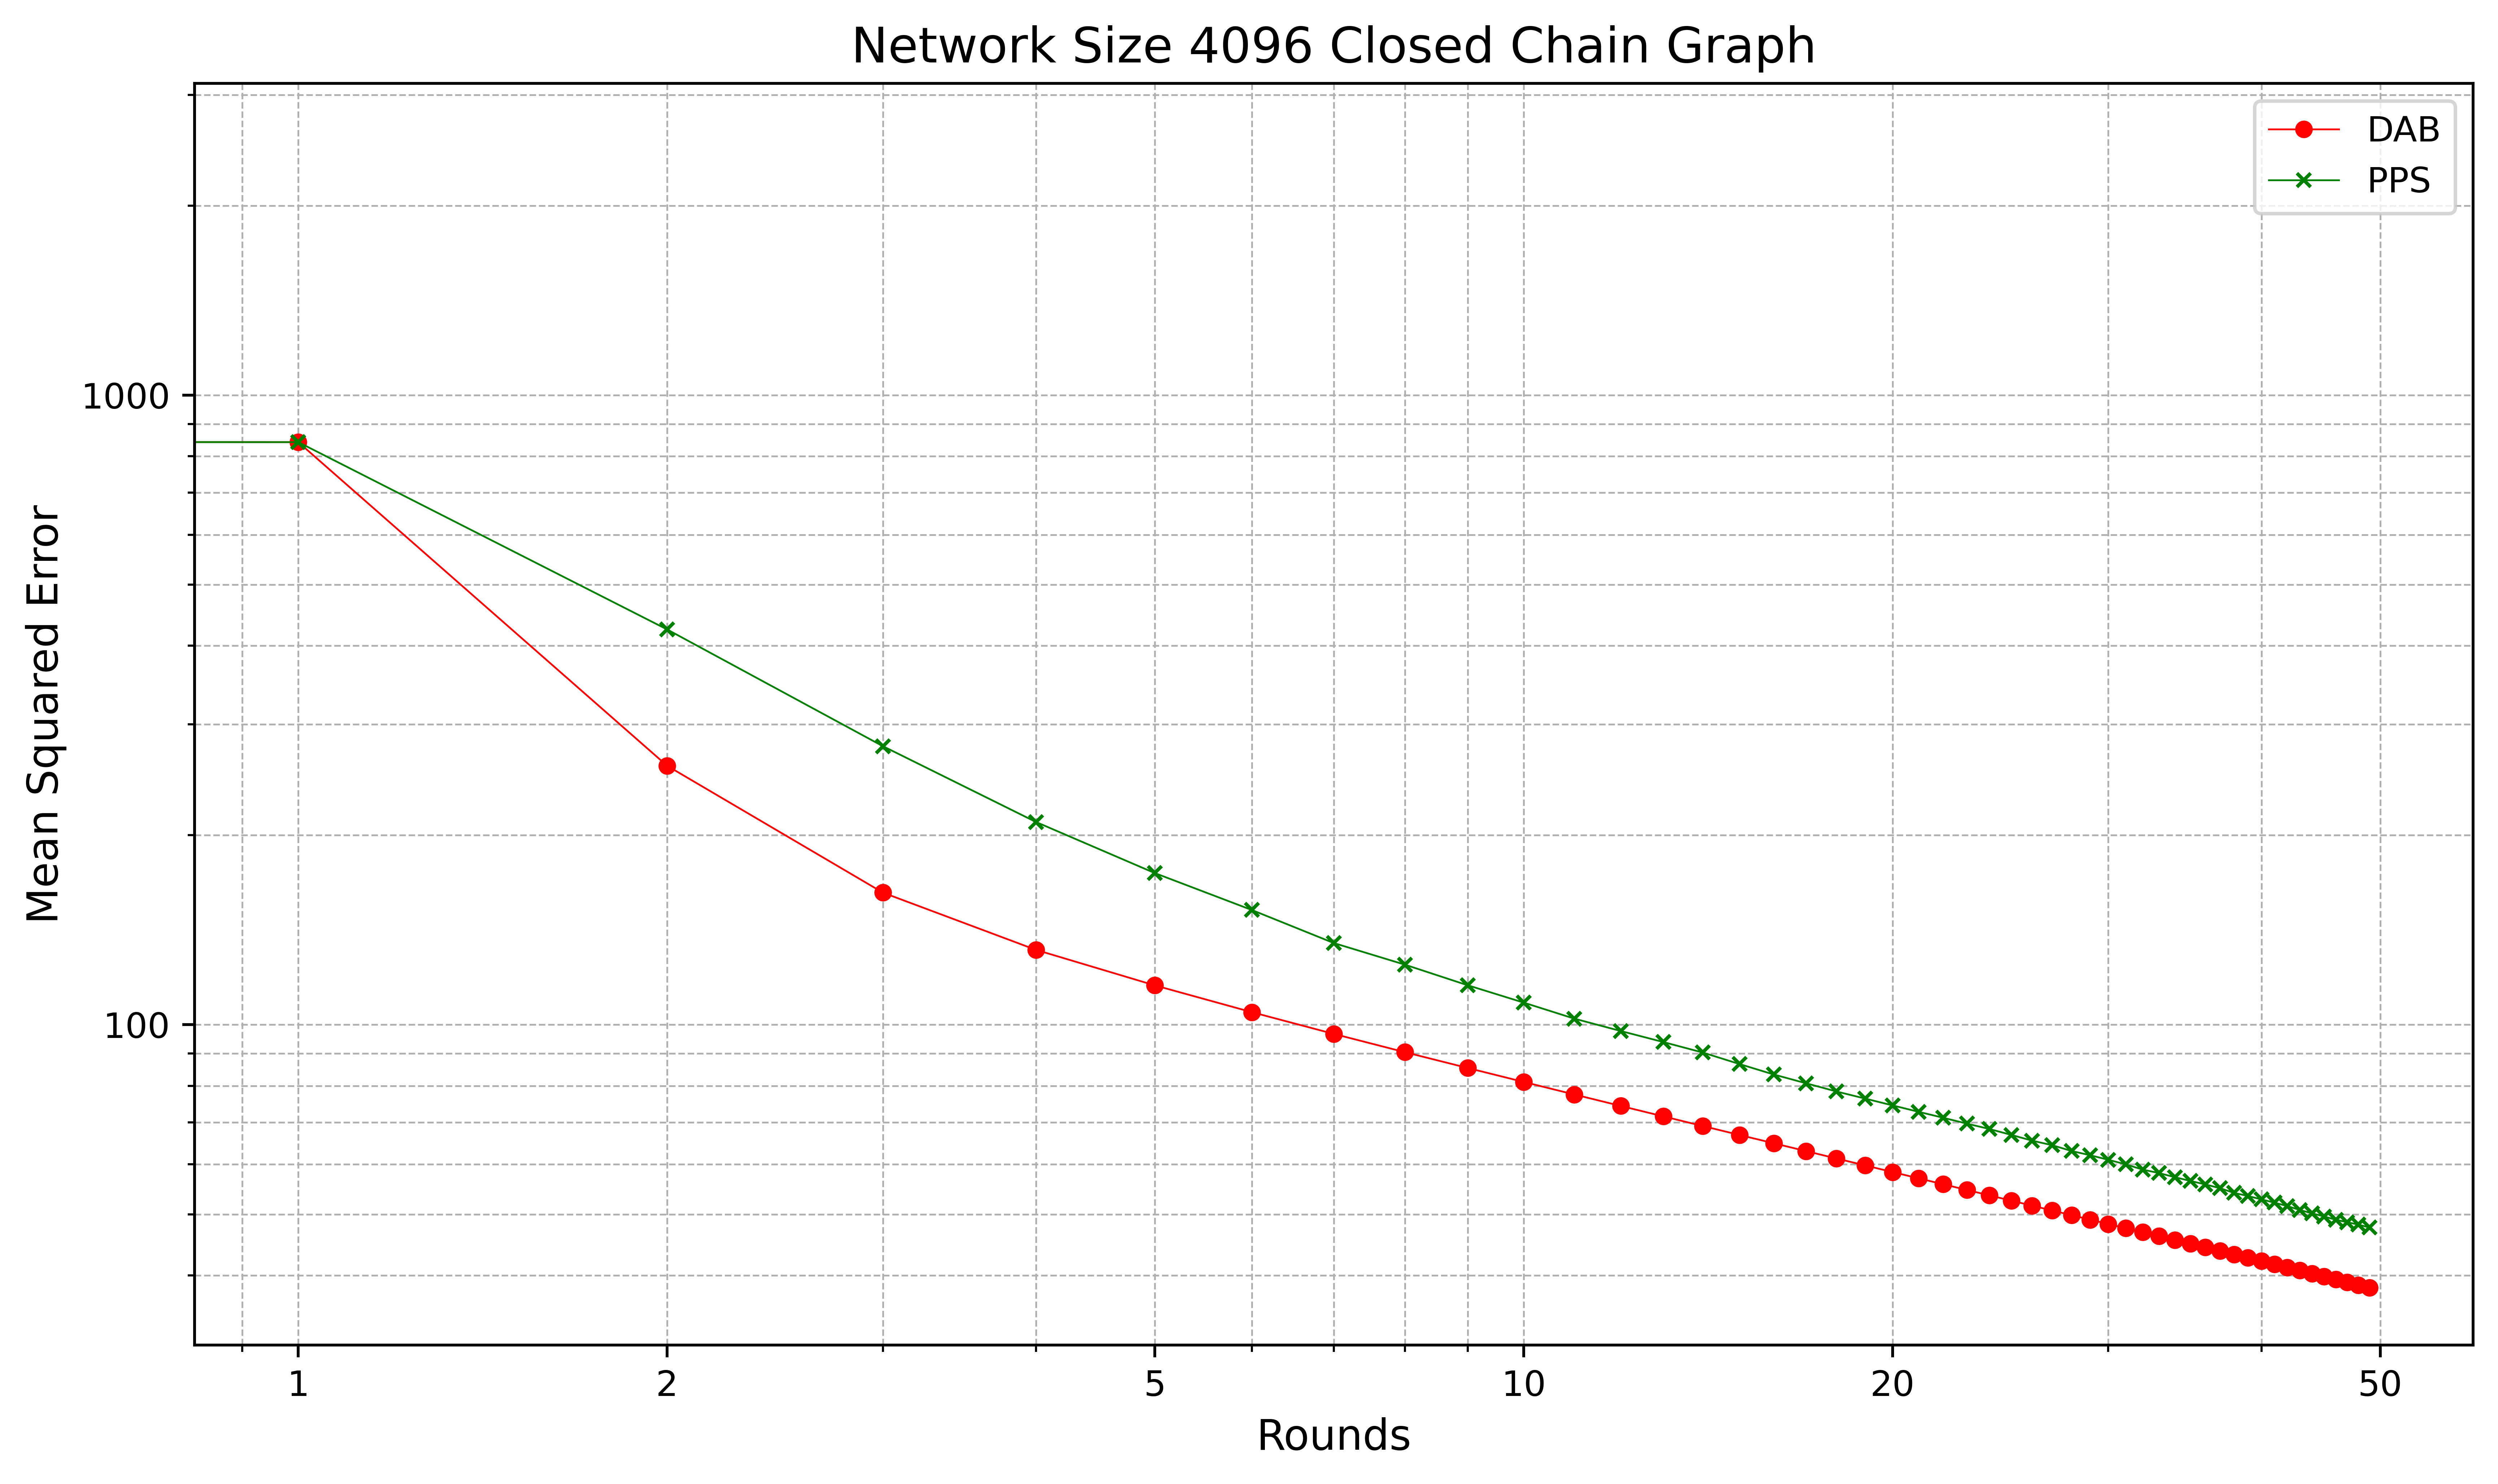
\includegraphics[scale=0.5]{figures/closedChainSimulations/DAB_vs_PPS_CCG_r50_n4096.png}
    \caption{Closed chain graph: network size $2^{12}$ nodes}
    \label{fig:4096ChainGraph}
\end{figure}

\begin{figure}[H]
    \centering
    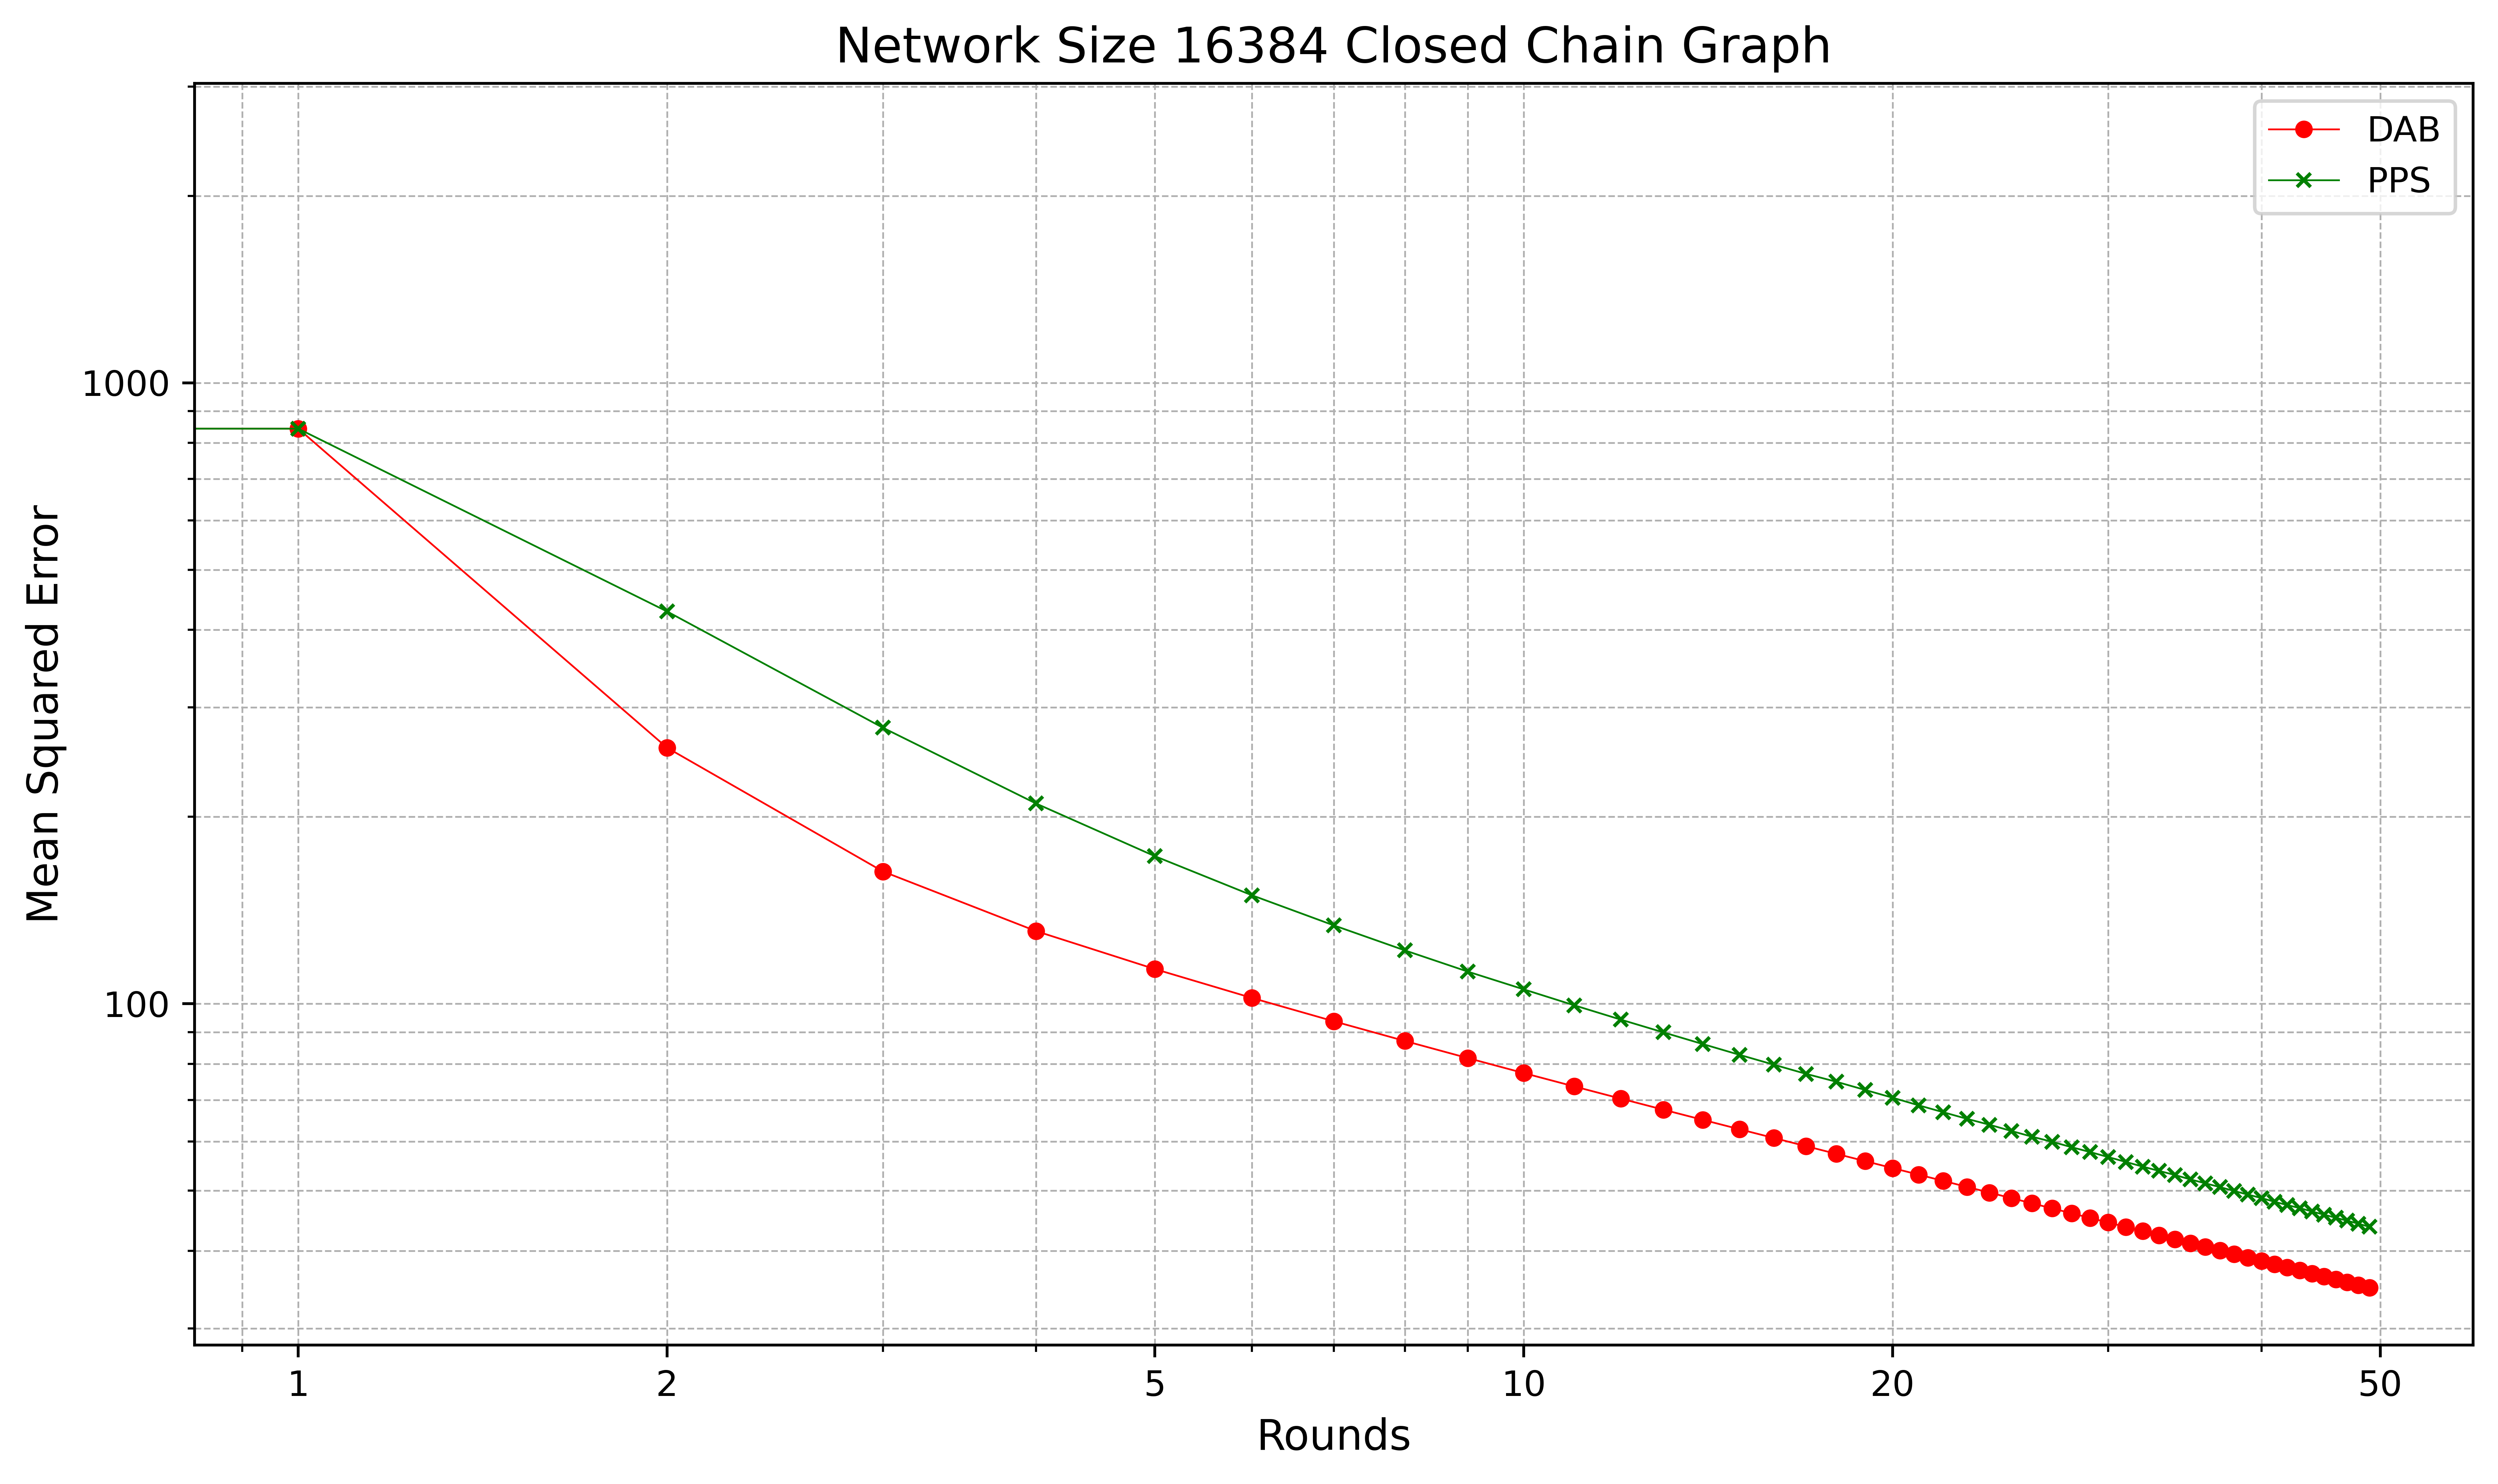
\includegraphics[scale=0.5]{figures/closedChainSimulations/DAB_vs_PPS_CCG_r50_n16384.png}
    \caption{Closed chain graph: network size $2^{14}$ nodes}
    \label{fig:16384ChainGraph}
\end{figure}

\section{Torus Grid Graph}
\begin{figure}
    \centering
    \scalebox{1.5}{\tikzset{
    block/.style={draw, fill=blue, circle, minimum size=3pt},
    arrow/.style={->},
    line/.style={-}
}

\begin{tikzpicture}[>=stealth',node distance=0.5cm]
    % Creating rows of blocks
    {[start chain]
        \node[on chain] (s0) {};
        \node[on chain] (s1) {};
        \node[on chain] (s2) {};
        \node[on chain] (s3) {};
        \node[on chain] (s4) {};
    }
    {[start chain]
        \node[block,on chain, below = 0.15 cm of s0] (A0) {};
        \node[block,on chain, join =by {line}] (A1) {};
        \node[block,on chain, join =by {line}] (A2) {};
        \node[block,on chain, join =by {line}] (A3) {};
    }
    {[start chain]
        \node[block,on chain, below = of A0] (B0) {};
        \node[block,on chain, join =by {line}] (B1) {};
        \node[block,on chain, join =by {line}] (B2) {};
        \node[block,on chain, join =by {line}] (B3) {};
    }
    {[start chain]
        \node[block,on chain, below = of B0] (C0) {};
        \node[block,on chain, join =by {line}] (C1) {};
        \node[block,on chain, join =by {line}] (C2) {};
        \node[block,on chain, join =by {line}] (C3) {};
    }
    {[start chain]
        \node[block,on chain, below = of C0] (D0) {};
        \node[block,on chain, join =by {line}] (D1) {};
        \node[block,on chain, join =by {line}] (D2) {};
        \node[block,on chain, join =by {line}] (D3) {};
    }

    % Drawing vertical lines
    \draw (A0) -- (B0) -- (C0) -- (D0); % -- (E0);
    \draw (A1) -- (B1) -- (C1) -- (D1); % -- (E1);
    \draw (A2) -- (B2) -- (C2) -- (D2); % -- (E2);
    \draw (A3) -- (B3) -- (C3) -- (D3); % -- (E3);
    % Drawing loop backs horizontal
    \draw (A0.west) -- ($(A0.west) - (0.15, 0)$);
    \draw ($(A0.west) - (0.15, 0)$) -- ($(A0.west) - (0.15, 0)+(0,0.5)$);
    \draw ($(A0.west) - (0.15, 0)+(0,0.5)$) -- ($(A0.west) +(3.1,0.5)$);
    \draw ($(A0.west) +(3.1,0.5)$) |- (A3.east);
    % \draw (A0.north) |- (s2.north east) -| (A4.north);
    % B row
    \draw (B0.west) -- ($(B0.west) - (0.15, 0)$);
    \draw ($(B0.west) - (0.15, 0)$) -- ($(B0.west) - (0.15, 0)+(0,0.5)$);
    \draw ($(B0.west) - (0.15, 0)+(0,0.5)$) -- ($(B0.west) +(3.1,0.5)$);
    \draw ($(B0.west) +(3.1,0.5)$) |- (B3.east);
    % C row
    \draw (C0.west) -- ($(C0.west) - (0.15, 0)$);
    \draw ($(C0.west) - (0.15, 0)$) -- ($(C0.west) - (0.15, 0)+(0,0.5)$);
    \draw ($(C0.west) - (0.15, 0)+(0,0.5)$) -- ($(C0.west) +(3.1,0.5)$);
    \draw ($(C0.west) +(3.1,0.5)$) |- (C3.east);
    % D row
    \draw (D0.west) -- ($(D0.west) - (0.15, 0)$);
    \draw ($(D0.west) - (0.15, 0)$) -- ($(D0.west) - (0.15, 0)+(0,0.5)$);
    \draw ($(D0.west) - (0.15, 0)+(0,0.5)$) -- ($(D0.west) +(3.1,0.5)$);
    \draw ($(D0.west) +(3.1,0.5)$) |- (D3.east);

    % Vertical Loopbacks

    % 0 column
    \draw (A0.north) -- ($(A0.north) + (0.0, 0.15)$);
    \draw ($(A0.north) + (0, 0.15)$) -- ($(A0.north) + (0, 0.15)+(-0.5,0)$);
    \draw ($(A0.north) + (0, 0.15)+(-0.5,0)$) -- ($(D0.north) +(-0.5,-0.65)$);
    \draw ($(D0.north) +(-0.5,-0.65)$) -| (D0.south);
    % 1 column
    \draw (A1.north) -- ($(A1.north) + (0.0, 0.15)$);
    \draw ($(A1.north) + (0, 0.15)$) -- ($(A1.north) + (0, 0.15)+(-0.5,0)$);
    \draw ($(A1.north) + (0, 0.15)+(-0.5,0)$) -- ($(D1.north) +(-0.5,-0.65)$);
    \draw ($(D1.north) +(-0.5,-0.65)$) -| (D1.south);
    % 2 column
    \draw (A2.north) -- ($(A2.north) + (0.0, 0.15)$);
    \draw ($(A2.north) + (0, 0.15)$) -- ($(A2.north) + (0, 0.15)+(-0.5,0)$);
    \draw ($(A2.north) + (0, 0.15)+(-0.5,0)$) -- ($(D2.north) +(-0.5,-0.65)$);
    \draw ($(D2.north) +(-0.5,-0.65)$) -| (D2.south);

    % 3 column
    \draw (A3.north) -- ($(A3.north) + (0.0, 0.15)$);
    \draw ($(A3.north) + (0, 0.15)$) -- ($(A3.north) + (0, 0.15)+(-0.5,0)$);
    \draw ($(A3.north) + (0, 0.15)+(-0.5,0)$) -- ($(D3.north) +(-0.5,-0.65)$);
    \draw ($(D3.north) +(-0.5,-0.65)$) -| (D3.south);
    
    \end{tikzpicture}}
    \caption{Torus grid graph: network size 16}
    \label{fig:torusGraphDemo}
\end{figure}
\textbf{The torus grid graph}: \cite{PasdeloupTranslationOnGraphs2017}.
\section{Ring of Cliques}
\textbf{The ring of cliques}: \cite{Mahlmann2010}
\begin{figure}
    \centering
    \scalebox{1}{\newcommand\single[2]{
    \foreach \x in {1,...,#2}{
            \pgfmathsetmacro{\ang}{360/#2}
            \pgfmathparse{(\x-1)*\ang}
            \node[draw,fill=blue,circle,inner sep=3pt] (#1-\x) at (\pgfmathresult:10cm) {};
        }
    \foreach \x [count=\xi from 1] in {2,4}{
            \foreach \y in {2,4}{
                    \path (#1-\xi) edge[-] (#1-\y);
                    \path (#1-3) edge[-] (#1-\y);
                }
        }
}

\begin{tikzpicture}
    \begin{scope}[local bounding box=scope1]
    \end{scope}
    \foreach \s[count=\si from 0] in {0,90,...,360}{
            \begin{scope}[shift={($(scope1) +(\s:2)$)}, scale=0.1,rotate=\s+90]
                \single{\si}{4};
            \end{scope}
        }
    \foreach \i/\j in {1/2,2/3,3/4,4/1}
    \draw (\i-1)--(\j-3);
\end{tikzpicture}}
    \caption{Ring of cliques: network size 16}
    \label{fig:ringofcliquesDemo}
\end{figure}

\section{Lollipop Graph}
\textbf{The lollipop graph}: \cite{JonassonLollipopGraphs2000}
\begin{figure}
    \centering
    \scalebox{1}{\begin{tikzpicture}
    % Define the 8 vertices in a flat line
    \foreach \i in {1,...,9} {
      \node[draw, fill=blue, circle, minimum size=6pt] (v\i) at (\i, 0) {};
    }
    
    % Draw edges to connect each vertex to the next
    \foreach \i in {1,...,8} {
      \pgfmathtruncatemacro{\j}{\i+1}
      \draw (v\i) -- (v\j);
    }

    % Define additional vertices for the complete graph on v1, centered around v1
    \node[draw, fill=blue, circle, minimum size=6pt] (c1) at (0,1) {};
    \node[draw, fill=blue, circle, minimum size=6pt] (c2) at (0,-1) {};
    \node[draw, fill=blue, circle, minimum size=6pt] (c3) at (-1,2) {};
    \node[draw, fill=blue, circle, minimum size=6pt] (c4) at (-1,-2) {};
    \node[draw, fill=blue, circle, minimum size=6pt] (c5) at (-2,-1) {};
    \node[draw, fill=blue, circle, minimum size=6pt] (c6) at (-2,1) {};
    \node[draw, fill=blue, circle, minimum size=6pt] (c7) at (-3, 0) {};
    
    % Connect the complete graph nodes to v1
    \foreach \k in {1,2,3,4,5,6,7} {
      \draw (v1) -- (c\k);
    }

    % Draw edges between the new nodes to form a complete graph
    \foreach \a in {1,2,3,4,5,6,7} {
      \foreach \b in {\a,...,7} {
        \ifnum\a=\b\else
        \draw (c\a) -- (c\b);
        \fi
      }
    }

  \end{tikzpicture}}
    \caption{Lollipop graph: network size 16}
    \label{fig:lollipopgraphDemo}
\end{figure}
    \chapter{Conclusion}\label{chap:conclusion}
WWrite about that DAB able to balance perfectly MSE of 0. (complete graph and star graph). After some state of network DAB improves rapidly. PPS is other way around usually in beginning more impulsive and later in the end relatively slow. (lollipop graph). cliques and complete graphs favor PPS. PPS not anytime see star. Less connectivity favor DAB.
    \chapter{Acknowledgments}

First and foremost, I would like to thank...
\begin{itemize}
\item{advisers}
\item{examiner}
\item{person1 for the dataset}
\item{person2 for the great suggestion}
\item{proofreaders}
\end{itemize}
    \chapter{Appendix}\label{chap:appendix}
The appendix contains all the simulations that did not make it into the main part of this report. The simulations are appended to this document without comment.
\section{Simulations with powers of 10}
\subsection{Complete Graph}
\begin{figure}[H]
    \centering
    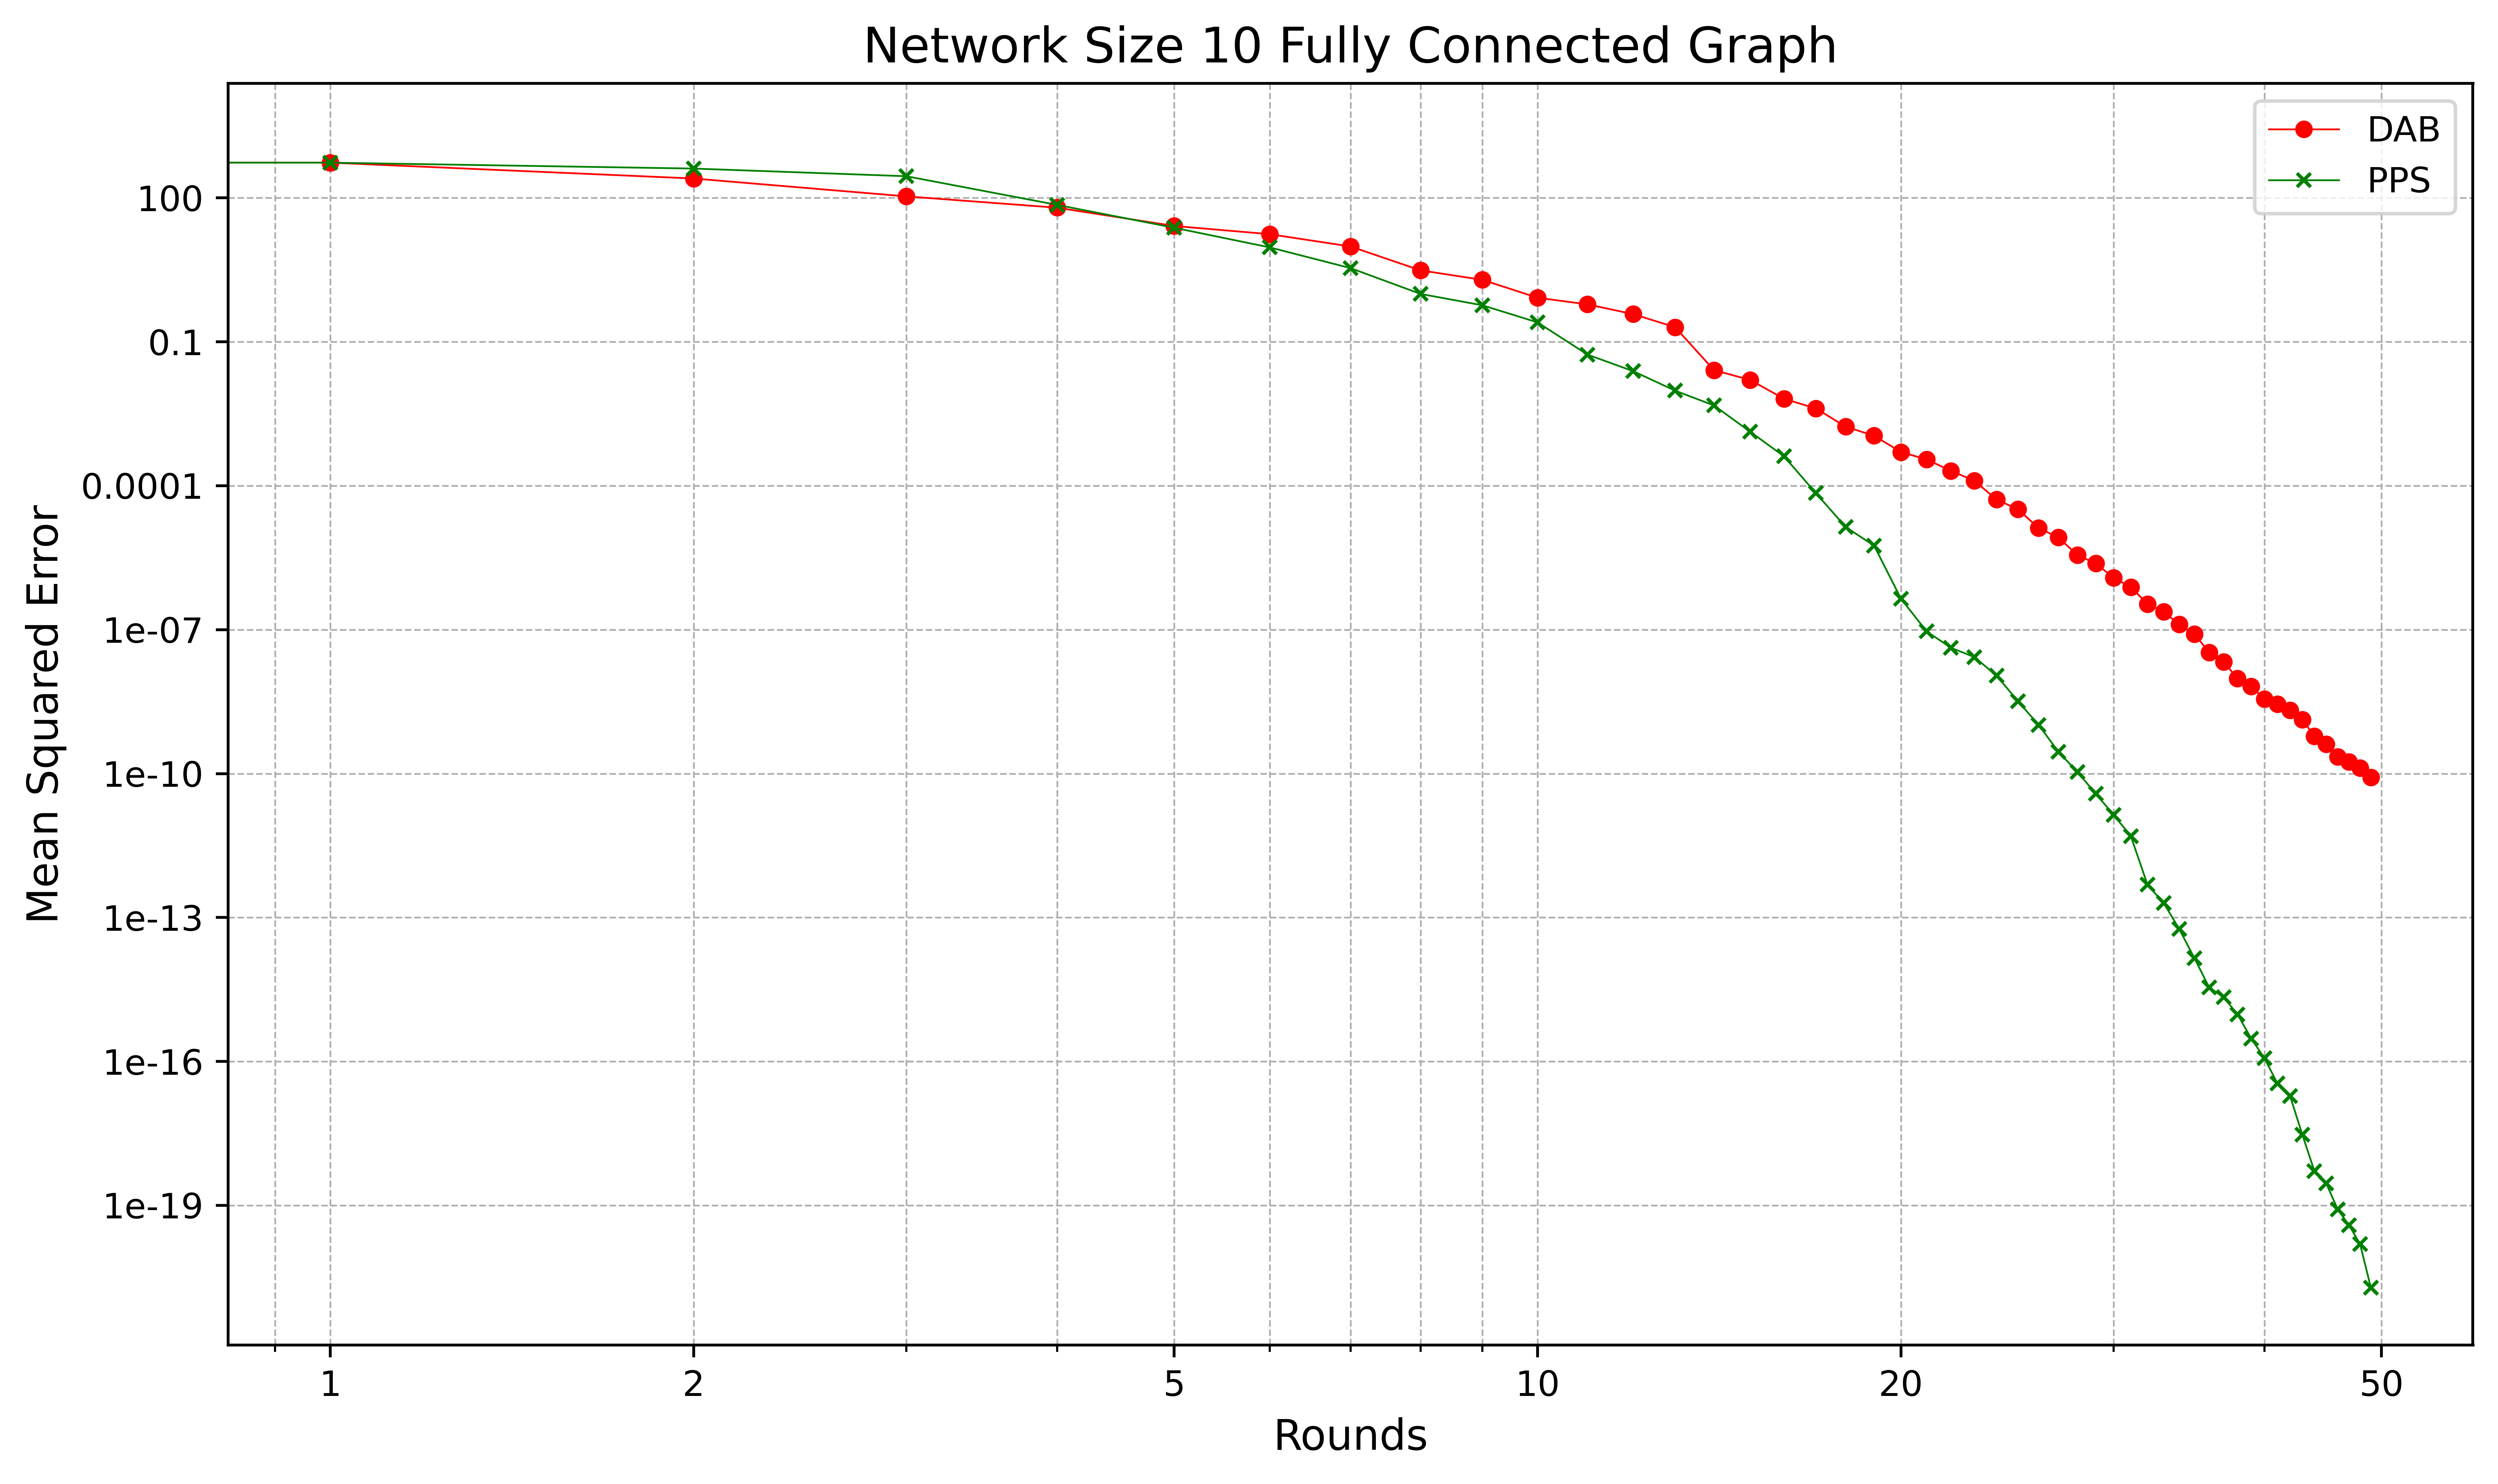
\includegraphics[scale=0.5]{figures/completeGraphSimulations/DAB_vs_PPS_FCG_r50_n10.png}
    \caption{Fully connected graph: network size $10^{1}$ nodes}
    \label{fig:10CompleteGraph}
\end{figure}
\begin{figure}[H]
    \centering
    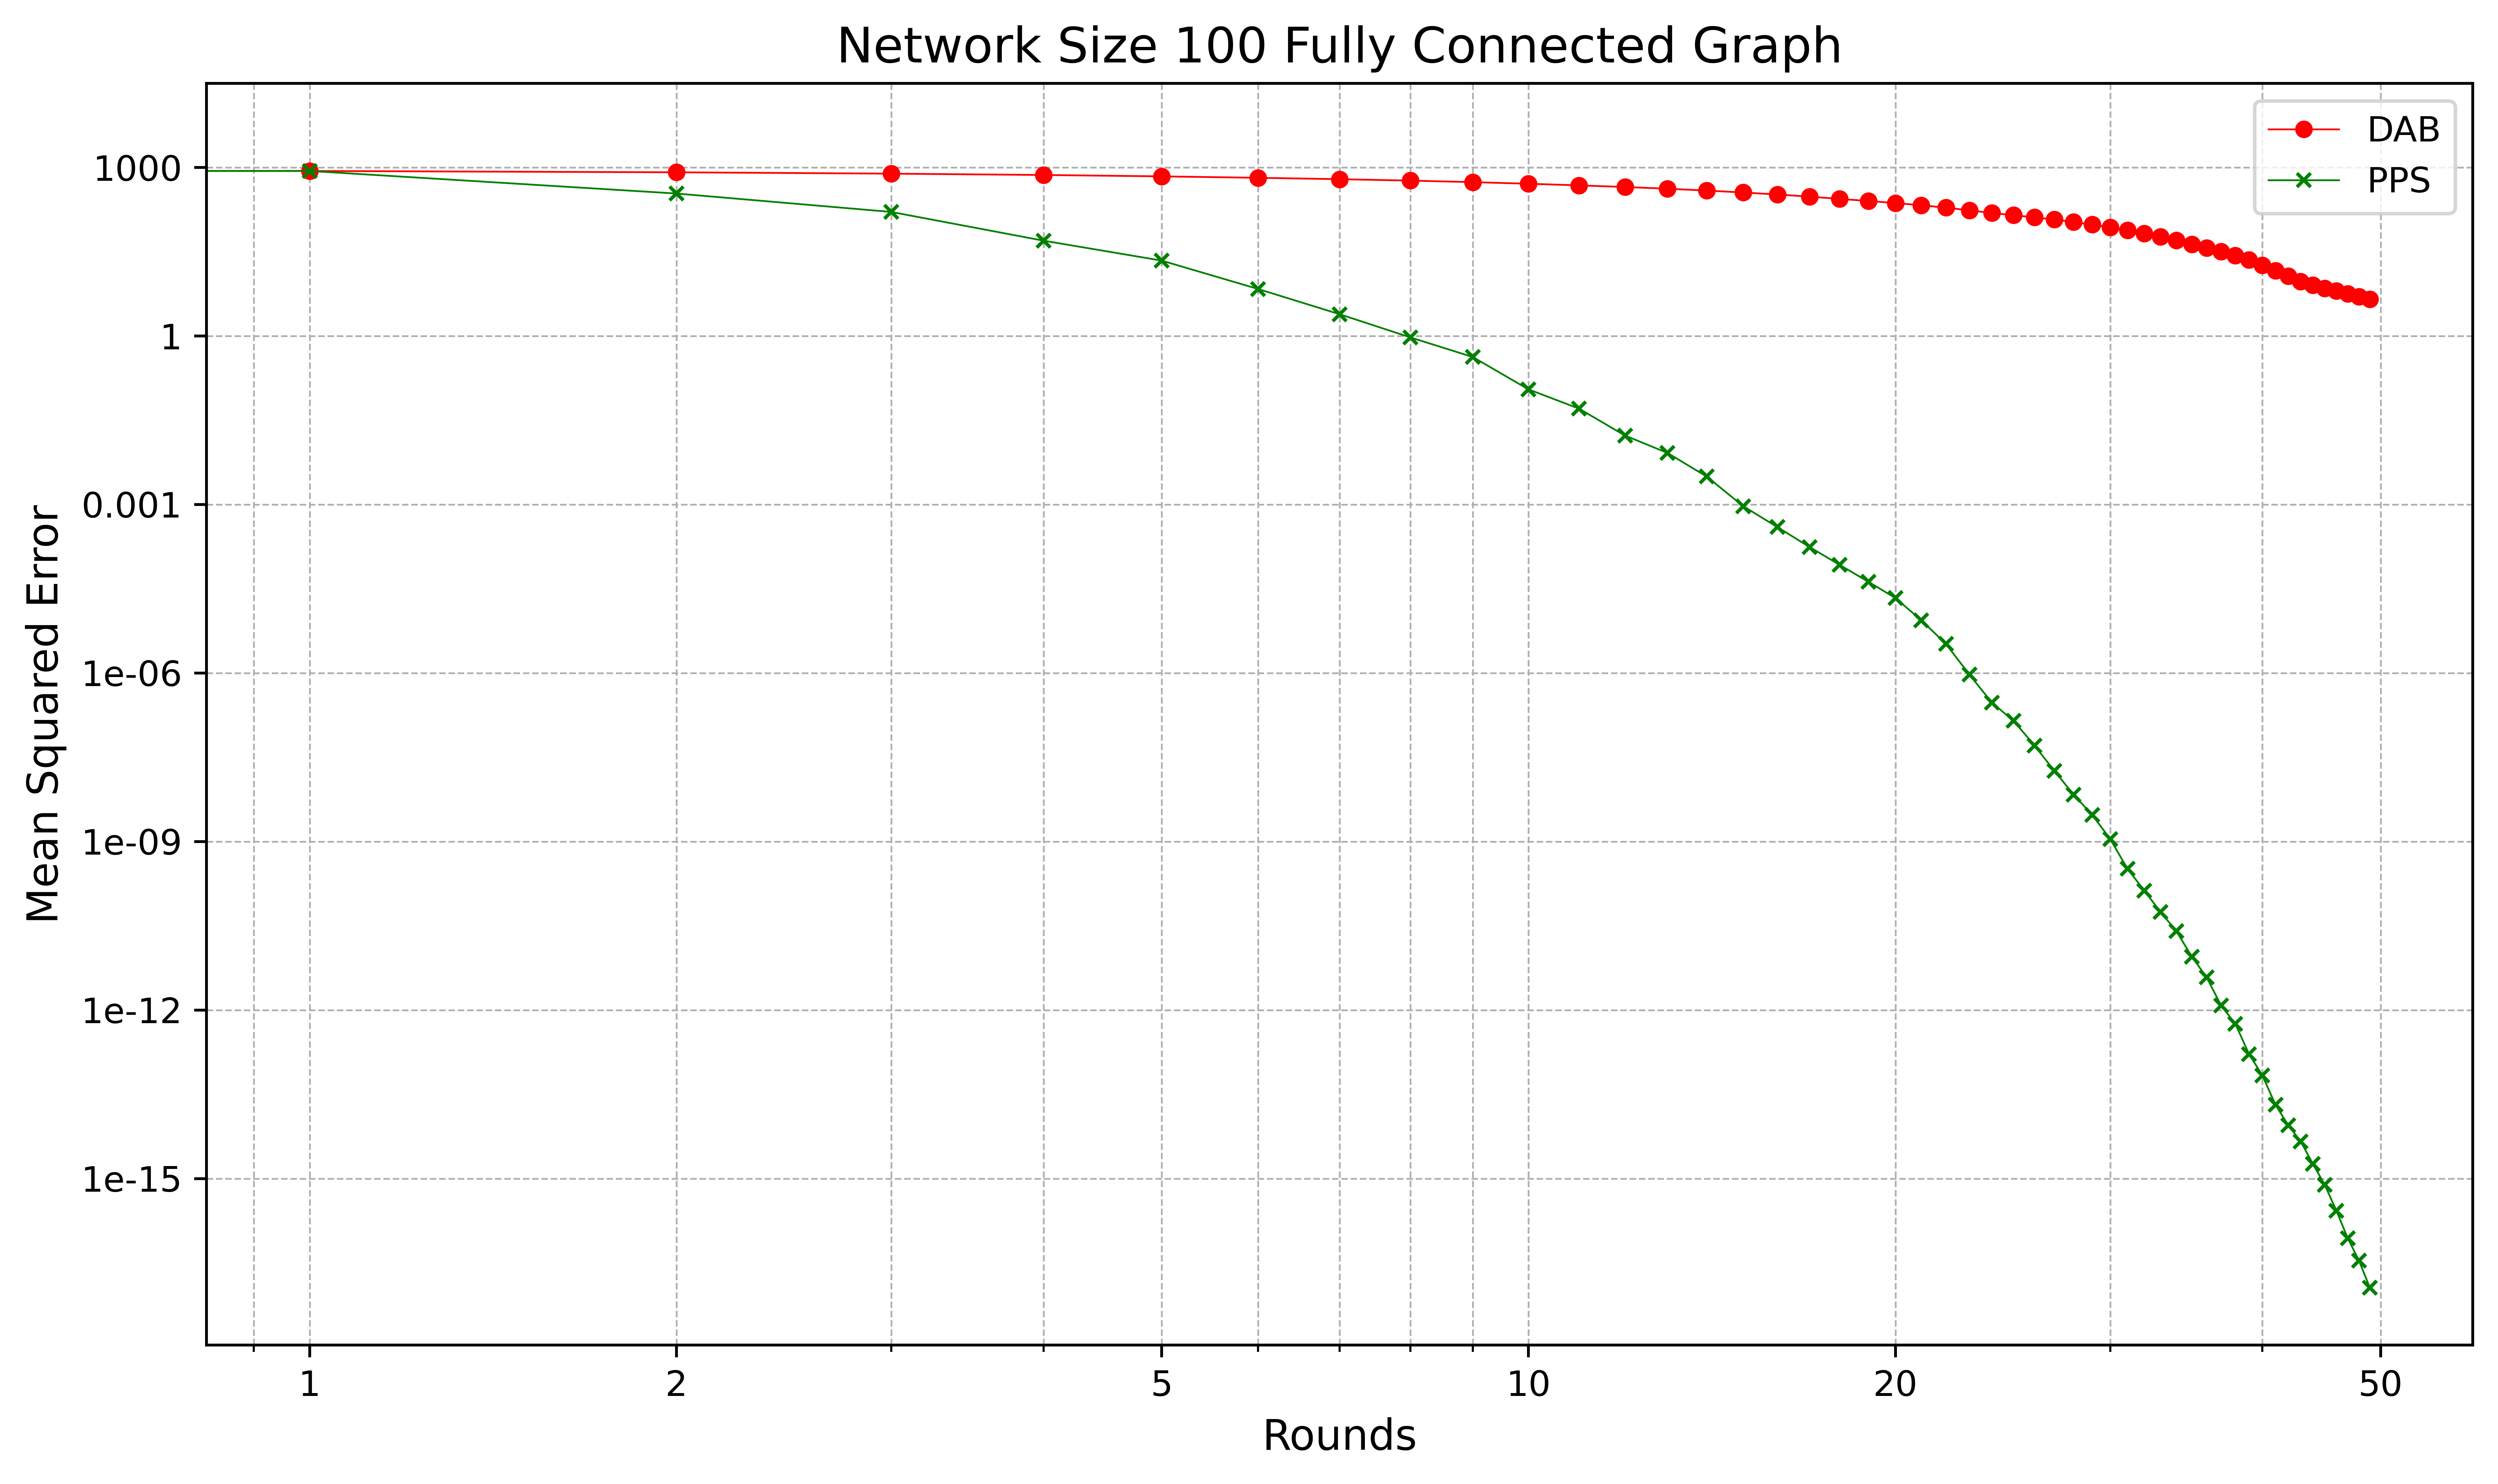
\includegraphics[scale=0.5]{figures/completeGraphSimulations/DAB_vs_PPS_FCG_r50_n100.png}
    \caption{Fully connected graph: network size $10^{2}$ nodes}
    \label{fig:100CompleteGraph}
\end{figure}
\begin{figure}[H]
    \centering
    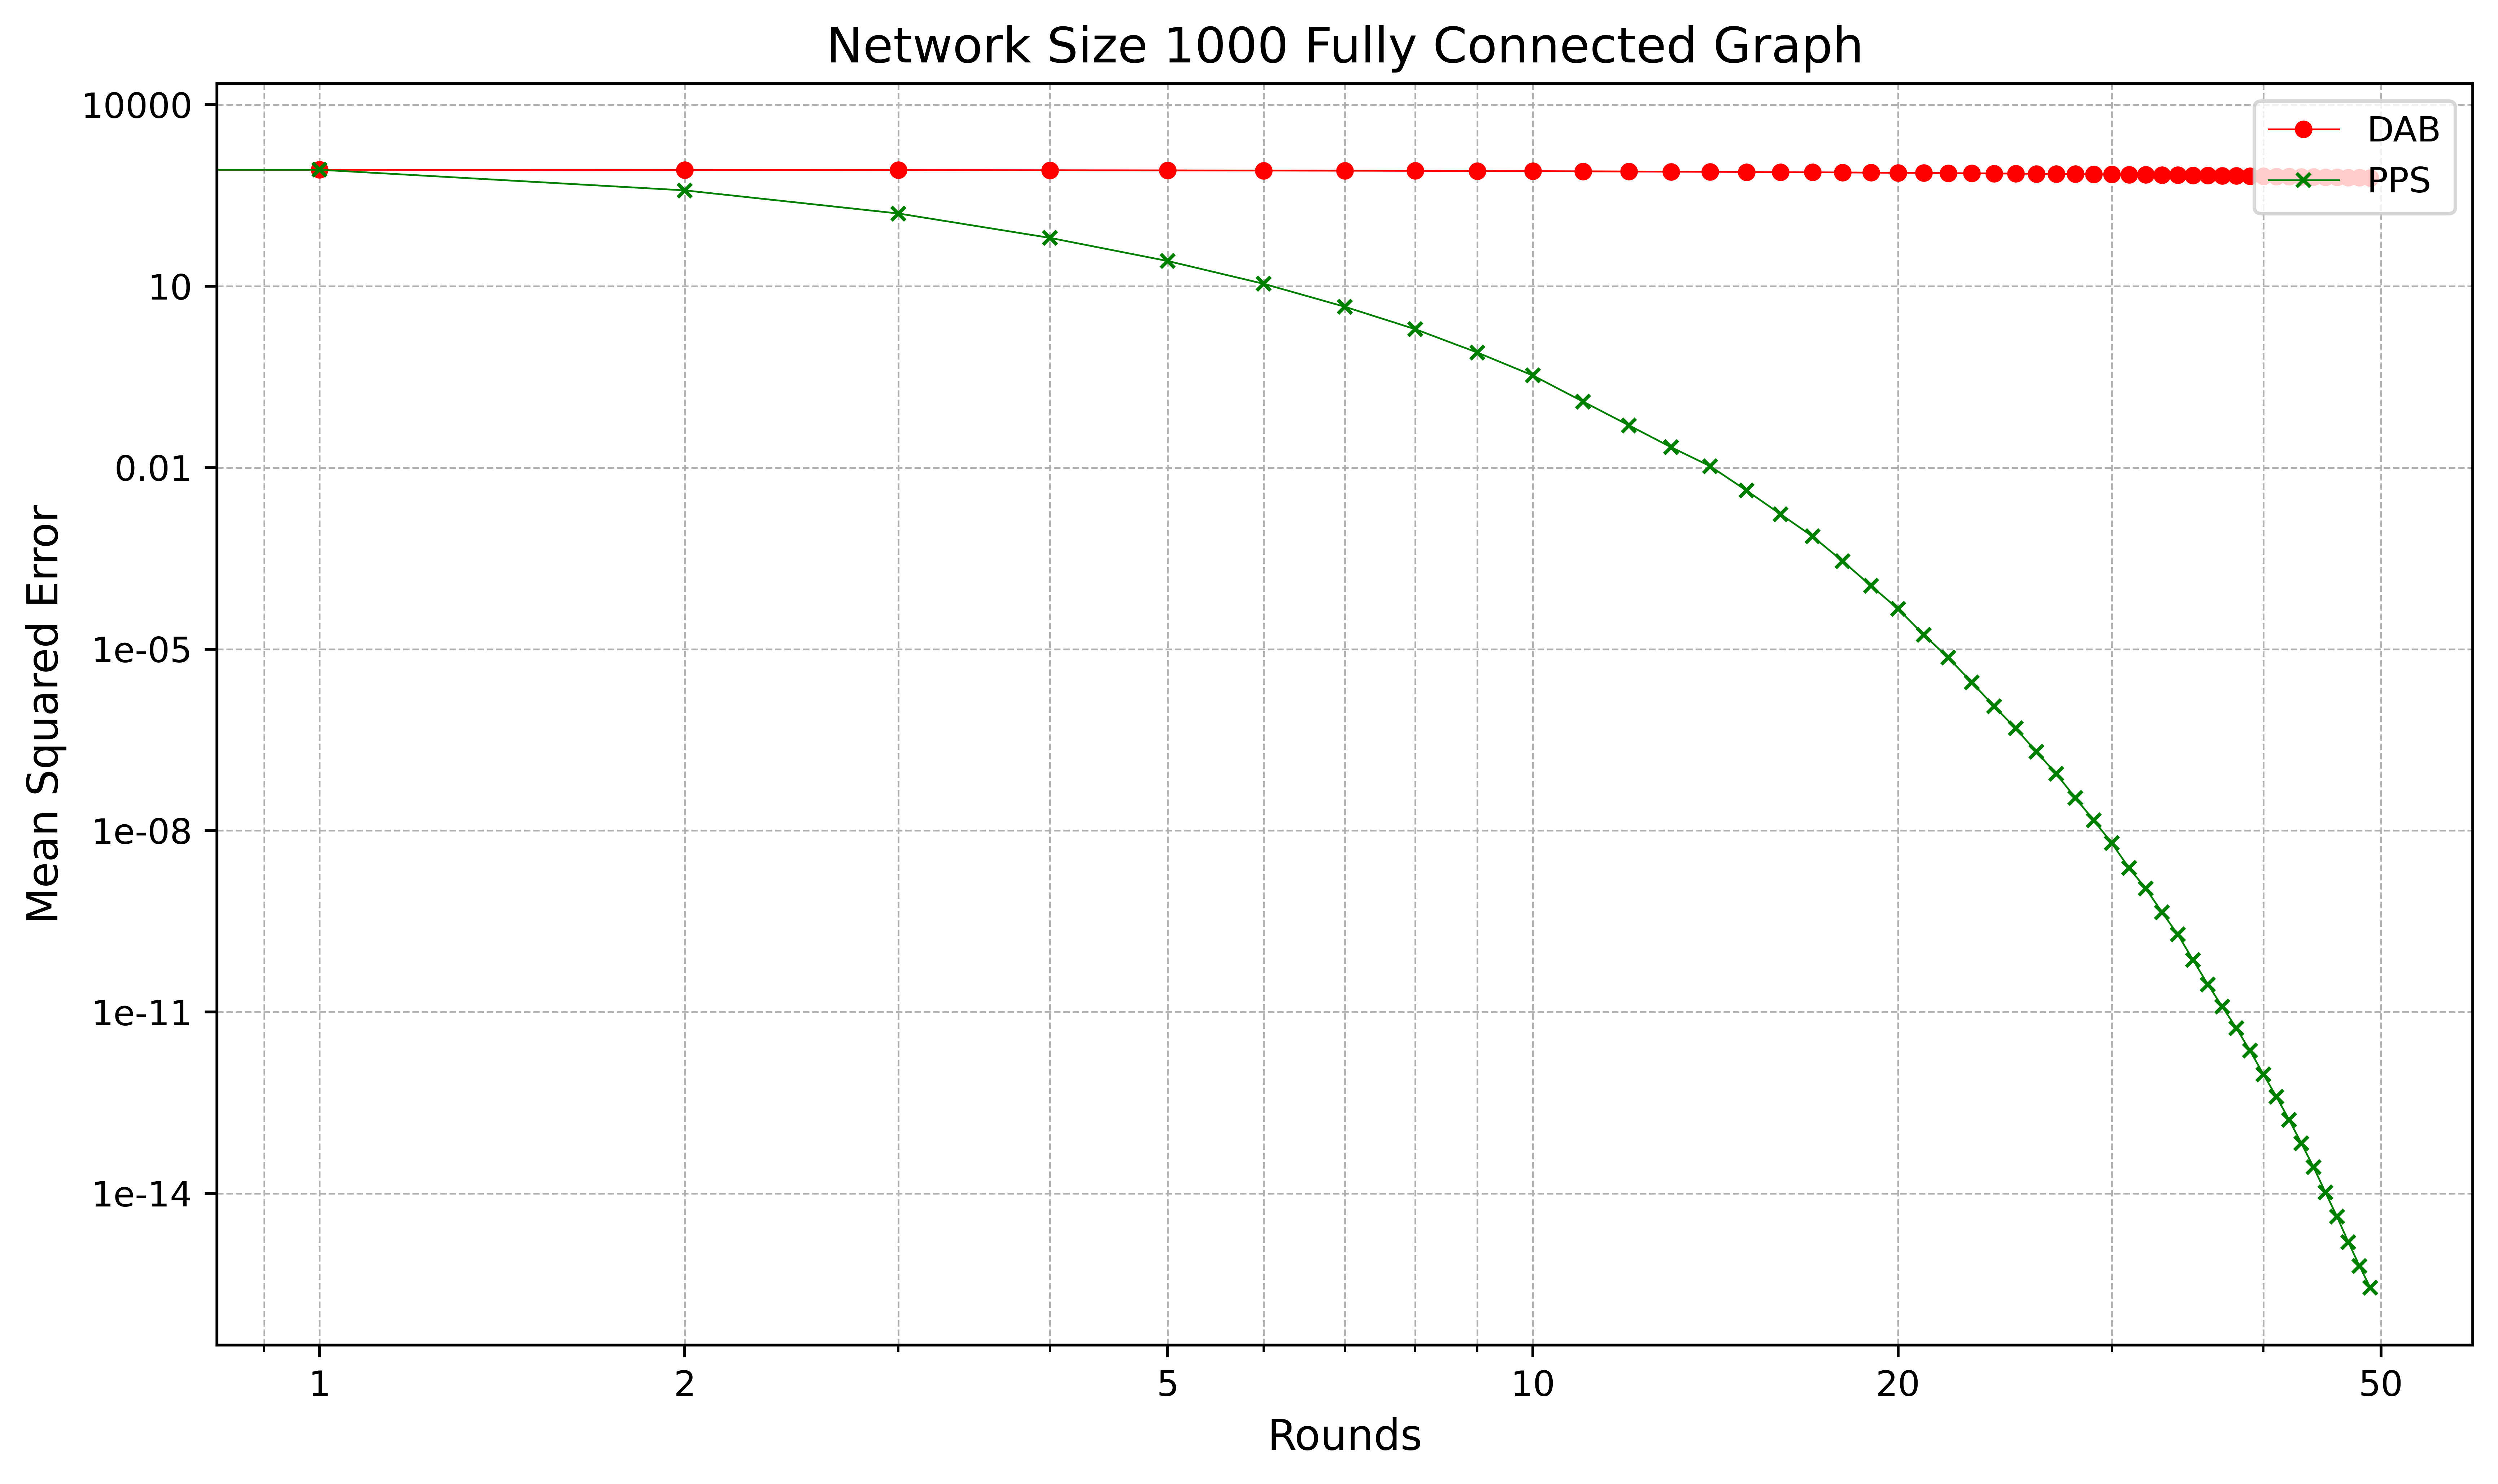
\includegraphics[scale=0.5]{figures/completeGraphSimulations/DAB_vs_PPS_FCG_r50_n1000.png}
    \caption{Fully connected graph: network size $10^{3}$ nodes}
    \label{fig:1000CompleteGraph}
\end{figure}
\begin{figure}[H]
    \centering
    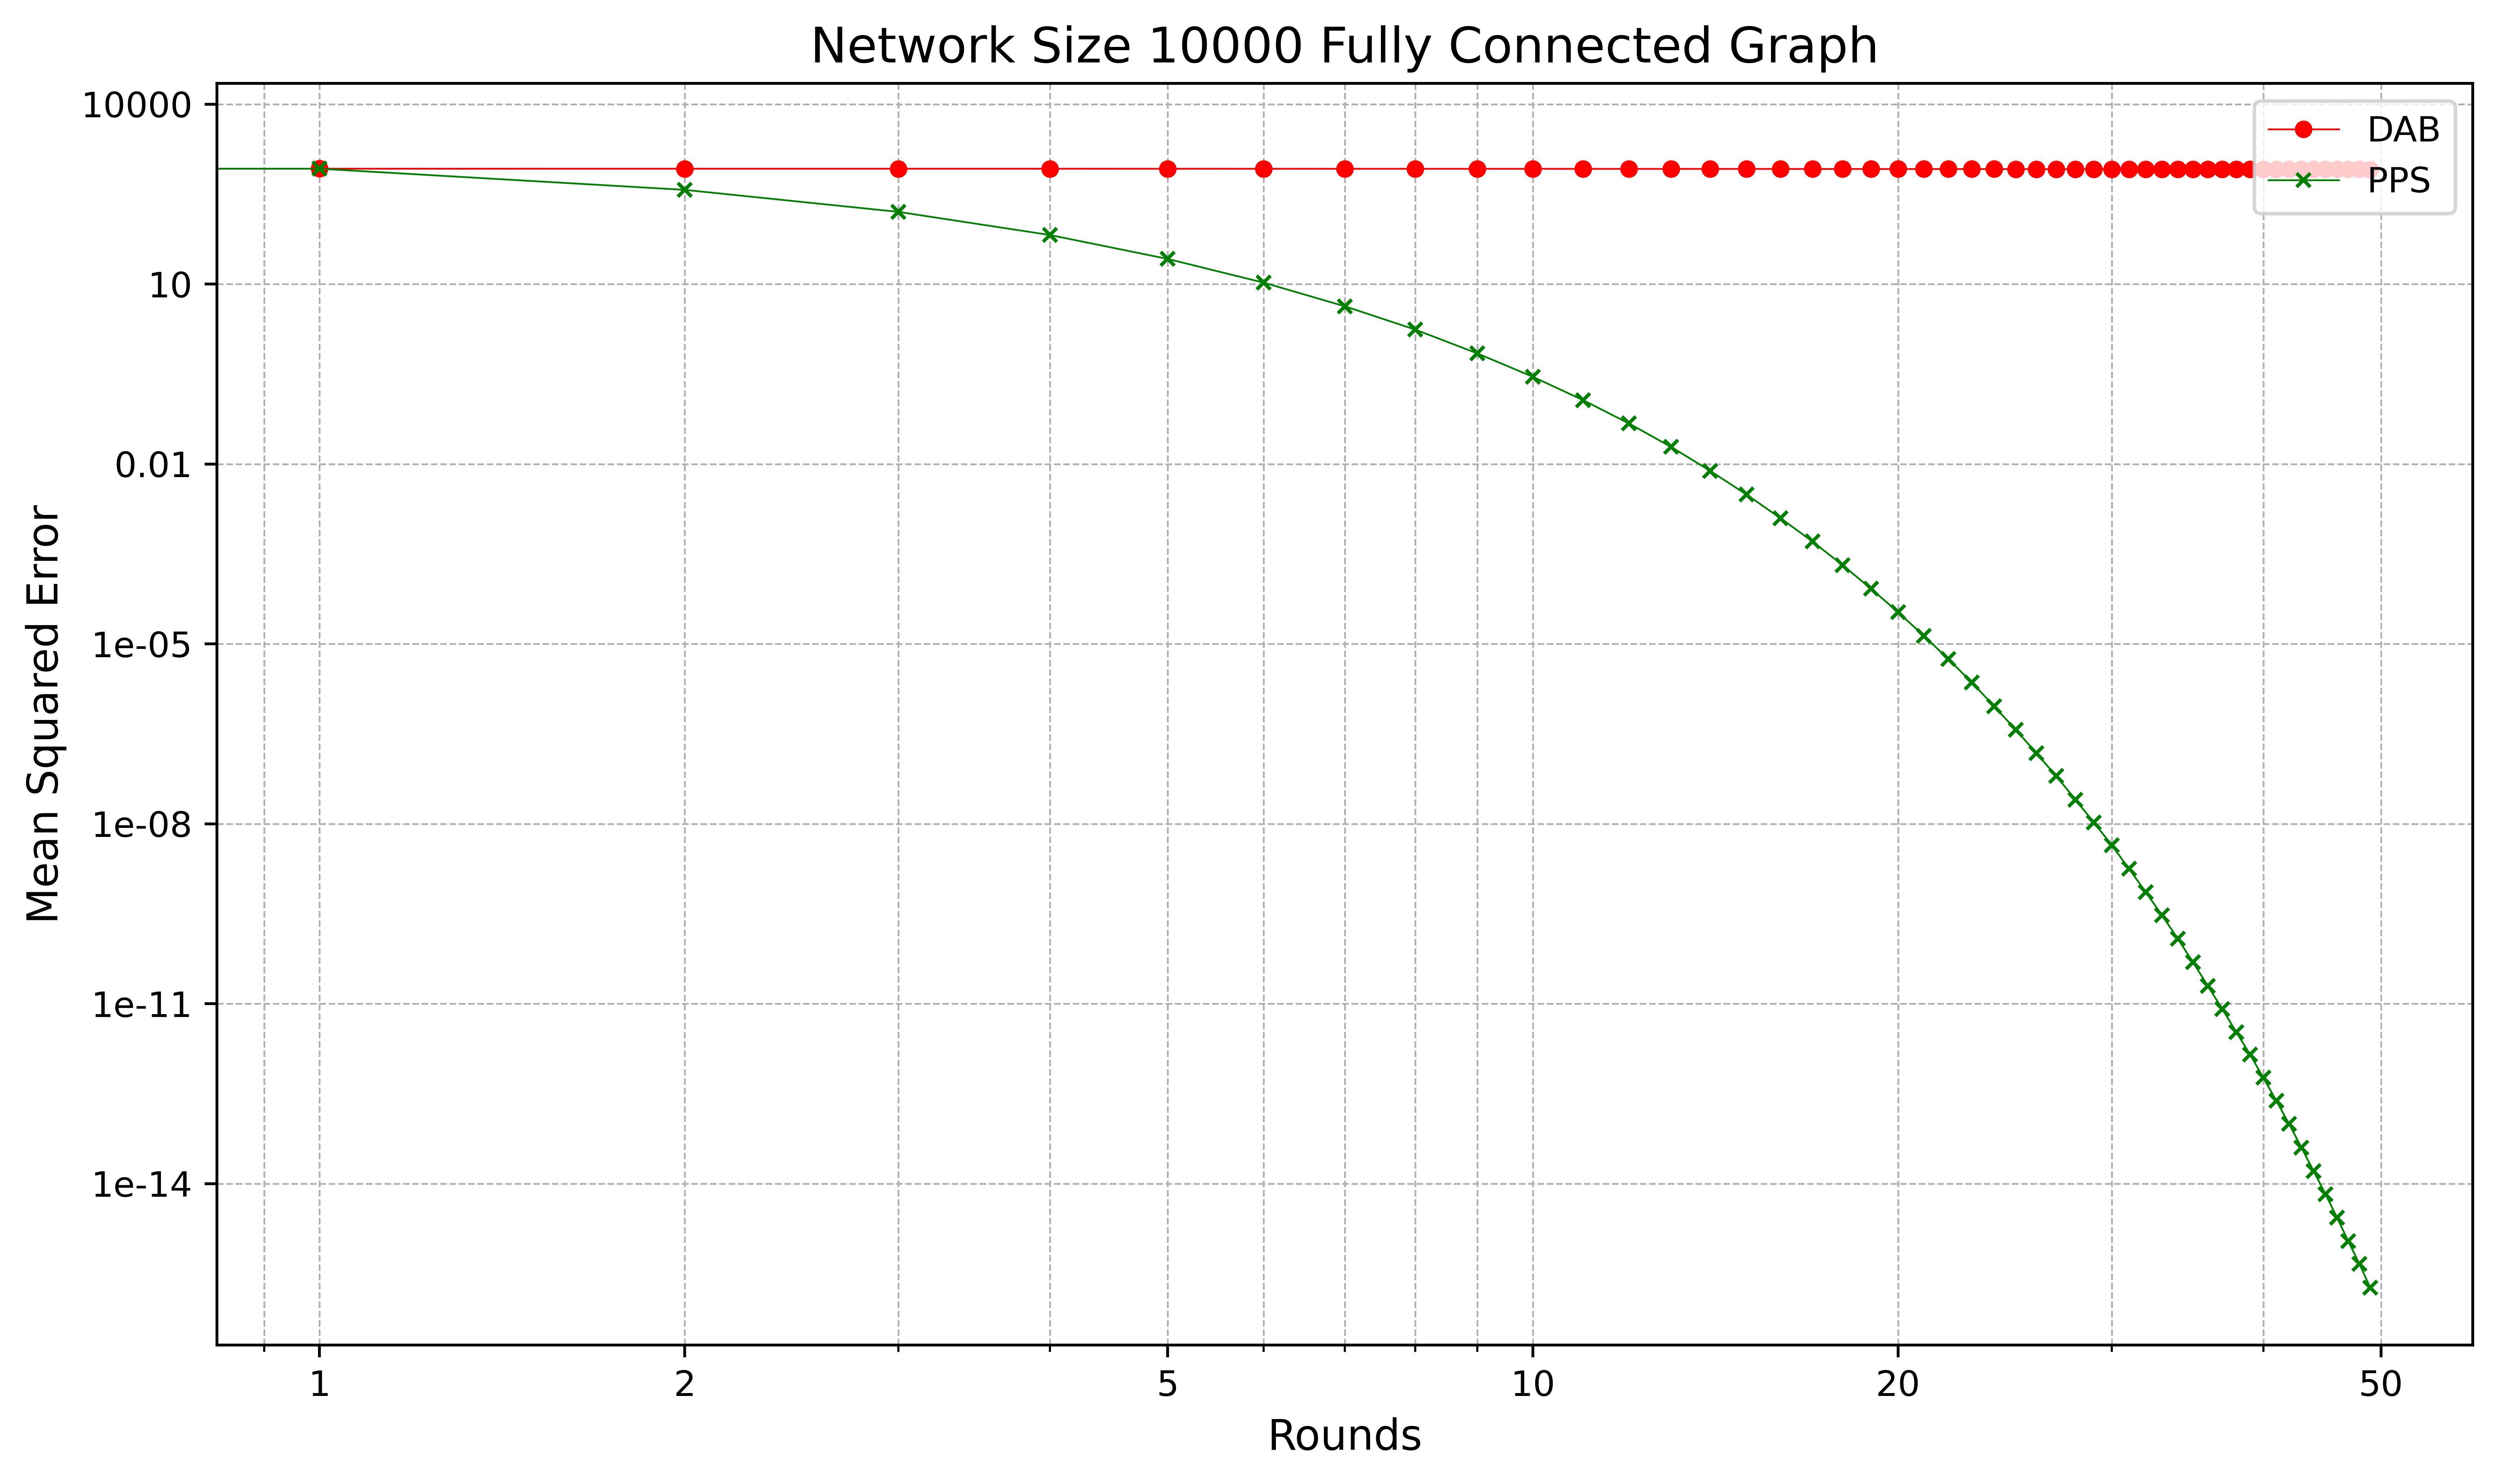
\includegraphics[scale=0.5]{figures/completeGraphSimulations/DAB_vs_PPS_FCG_r50_n10000.png}
    \caption{Fully connected graph: network size $10^{4}$ nodes}
    \label{fig:10000CompleteGraph}
\end{figure}

\subsection{Star Graph}
\begin{figure}[H]
    \centering
    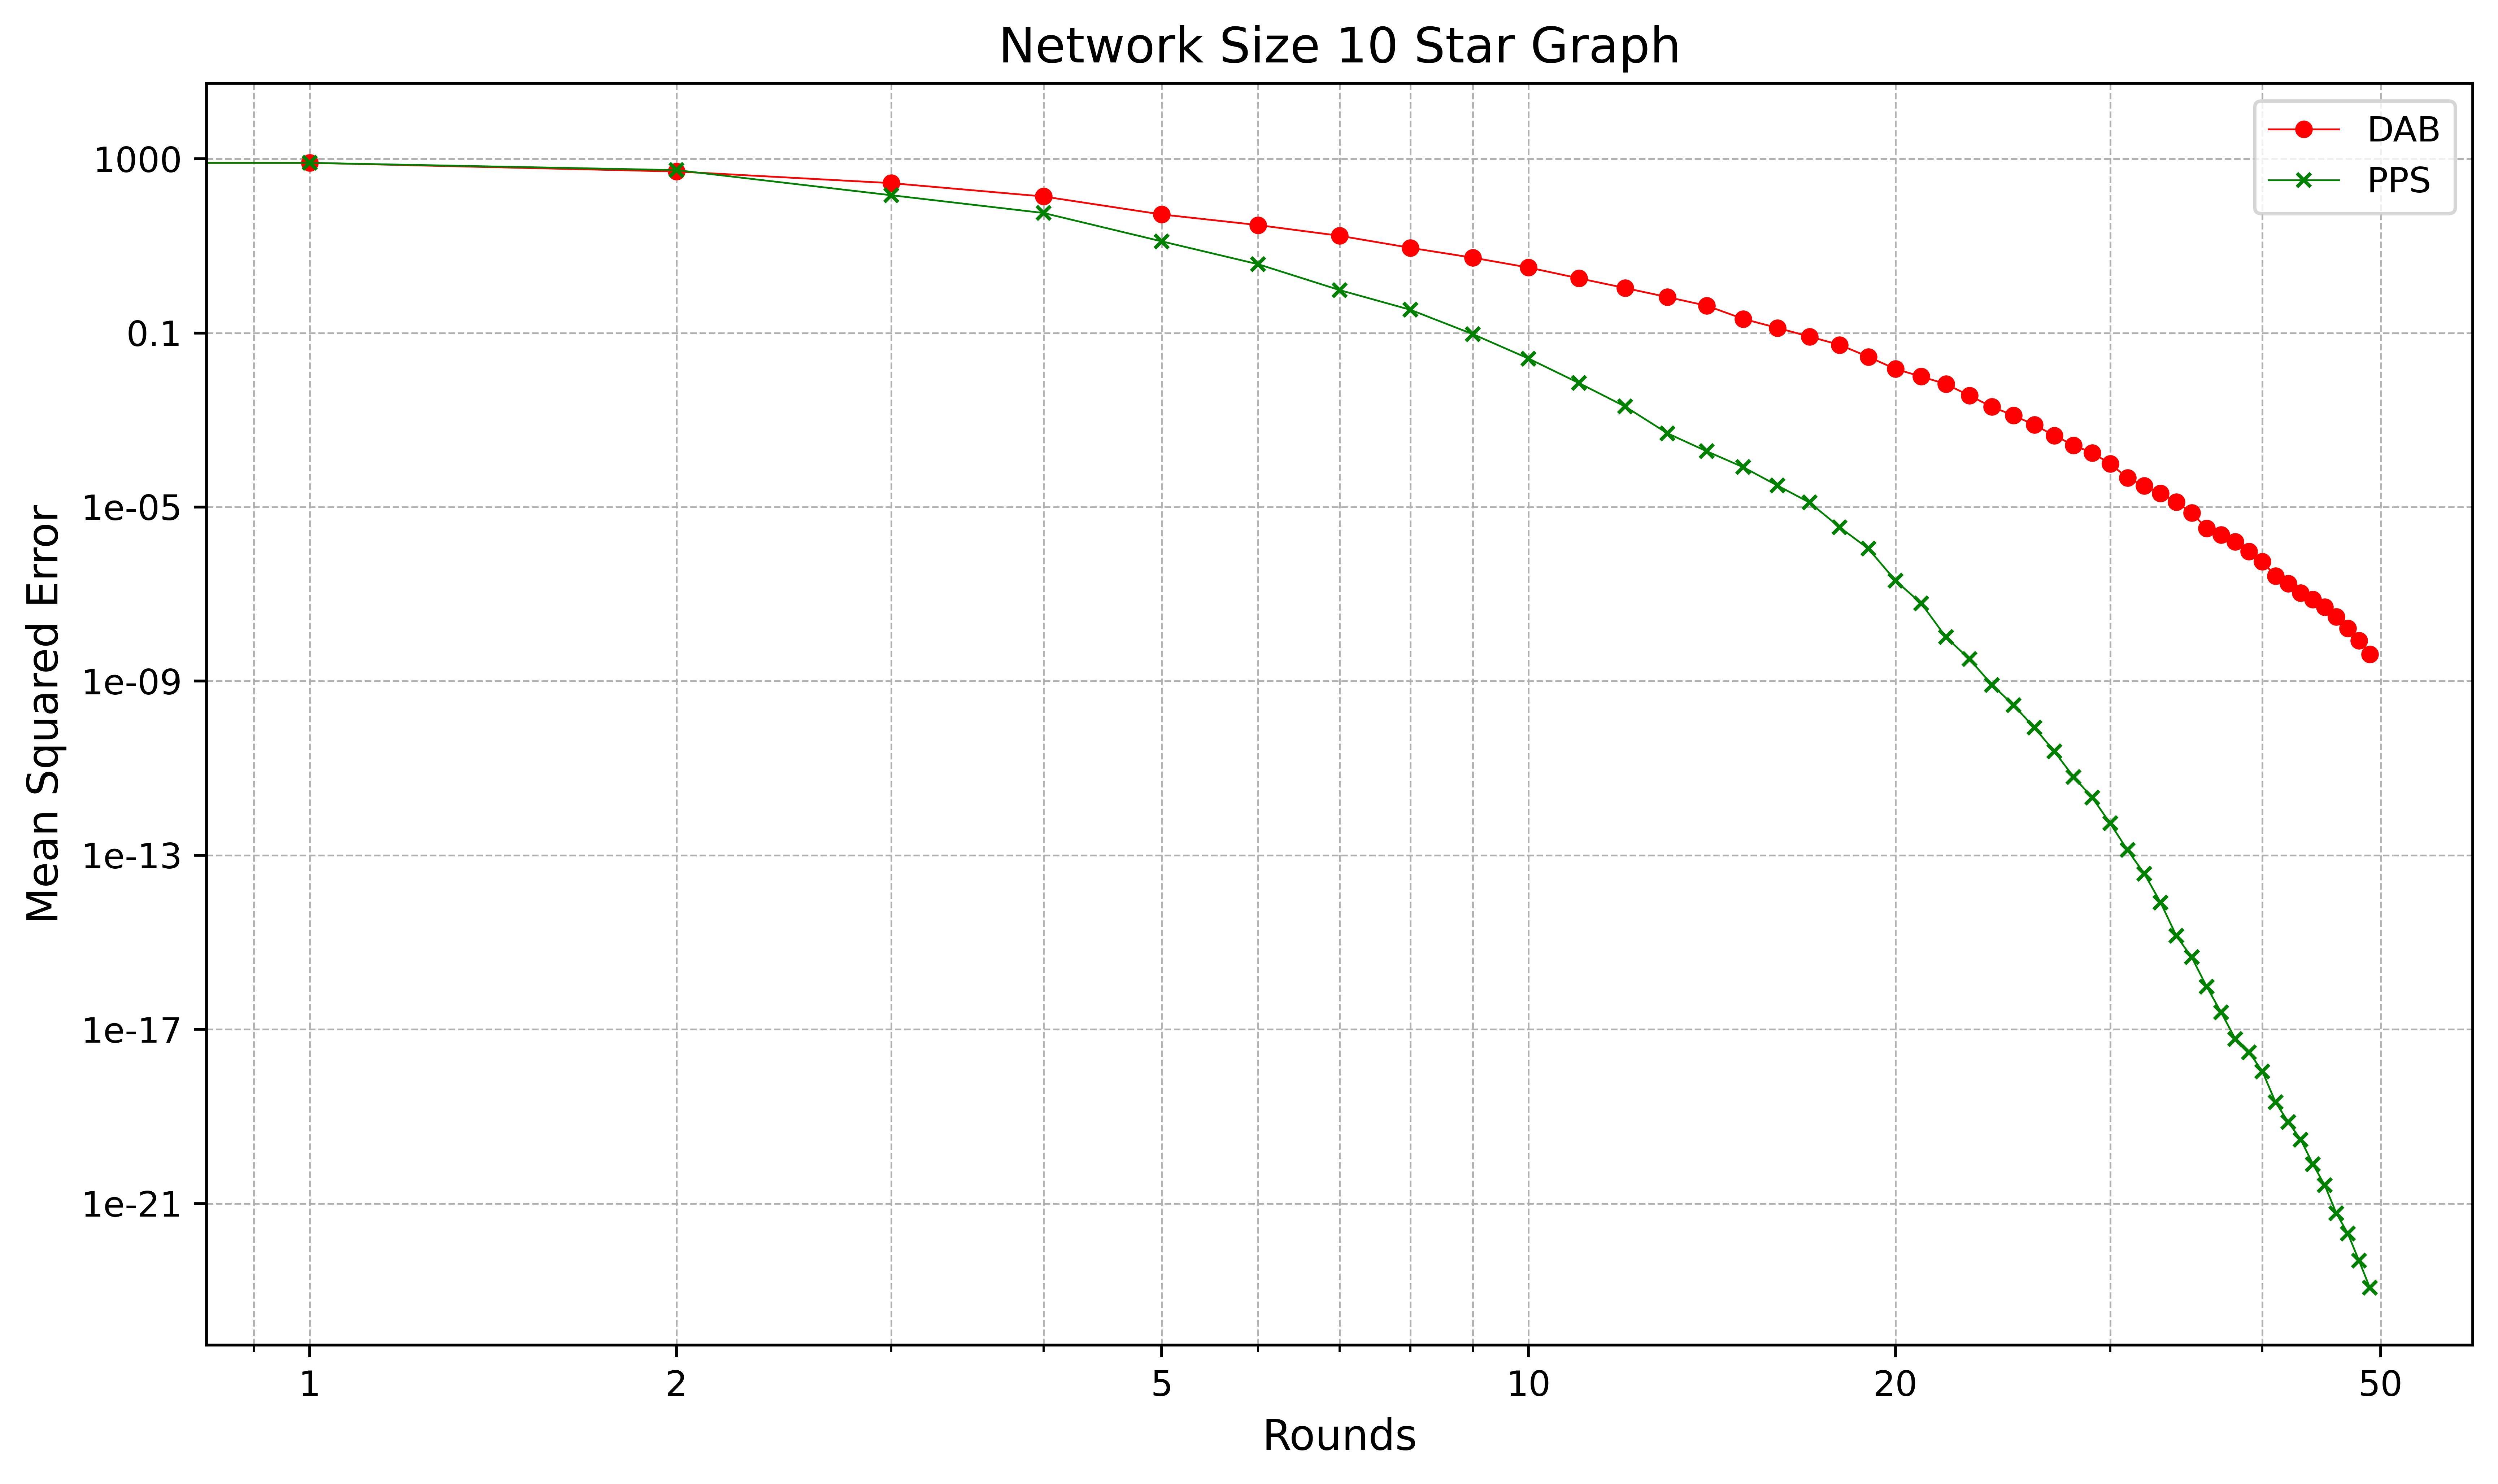
\includegraphics[scale=0.5]{figures/starGraphSimulations/DAB_vs_PPS_SG_r50_n10.png}
    \caption{Star graph: network size $10^{1}$ nodes}
    \label{fig:10StarGraph}
\end{figure}
\begin{figure}[H]
    \centering
    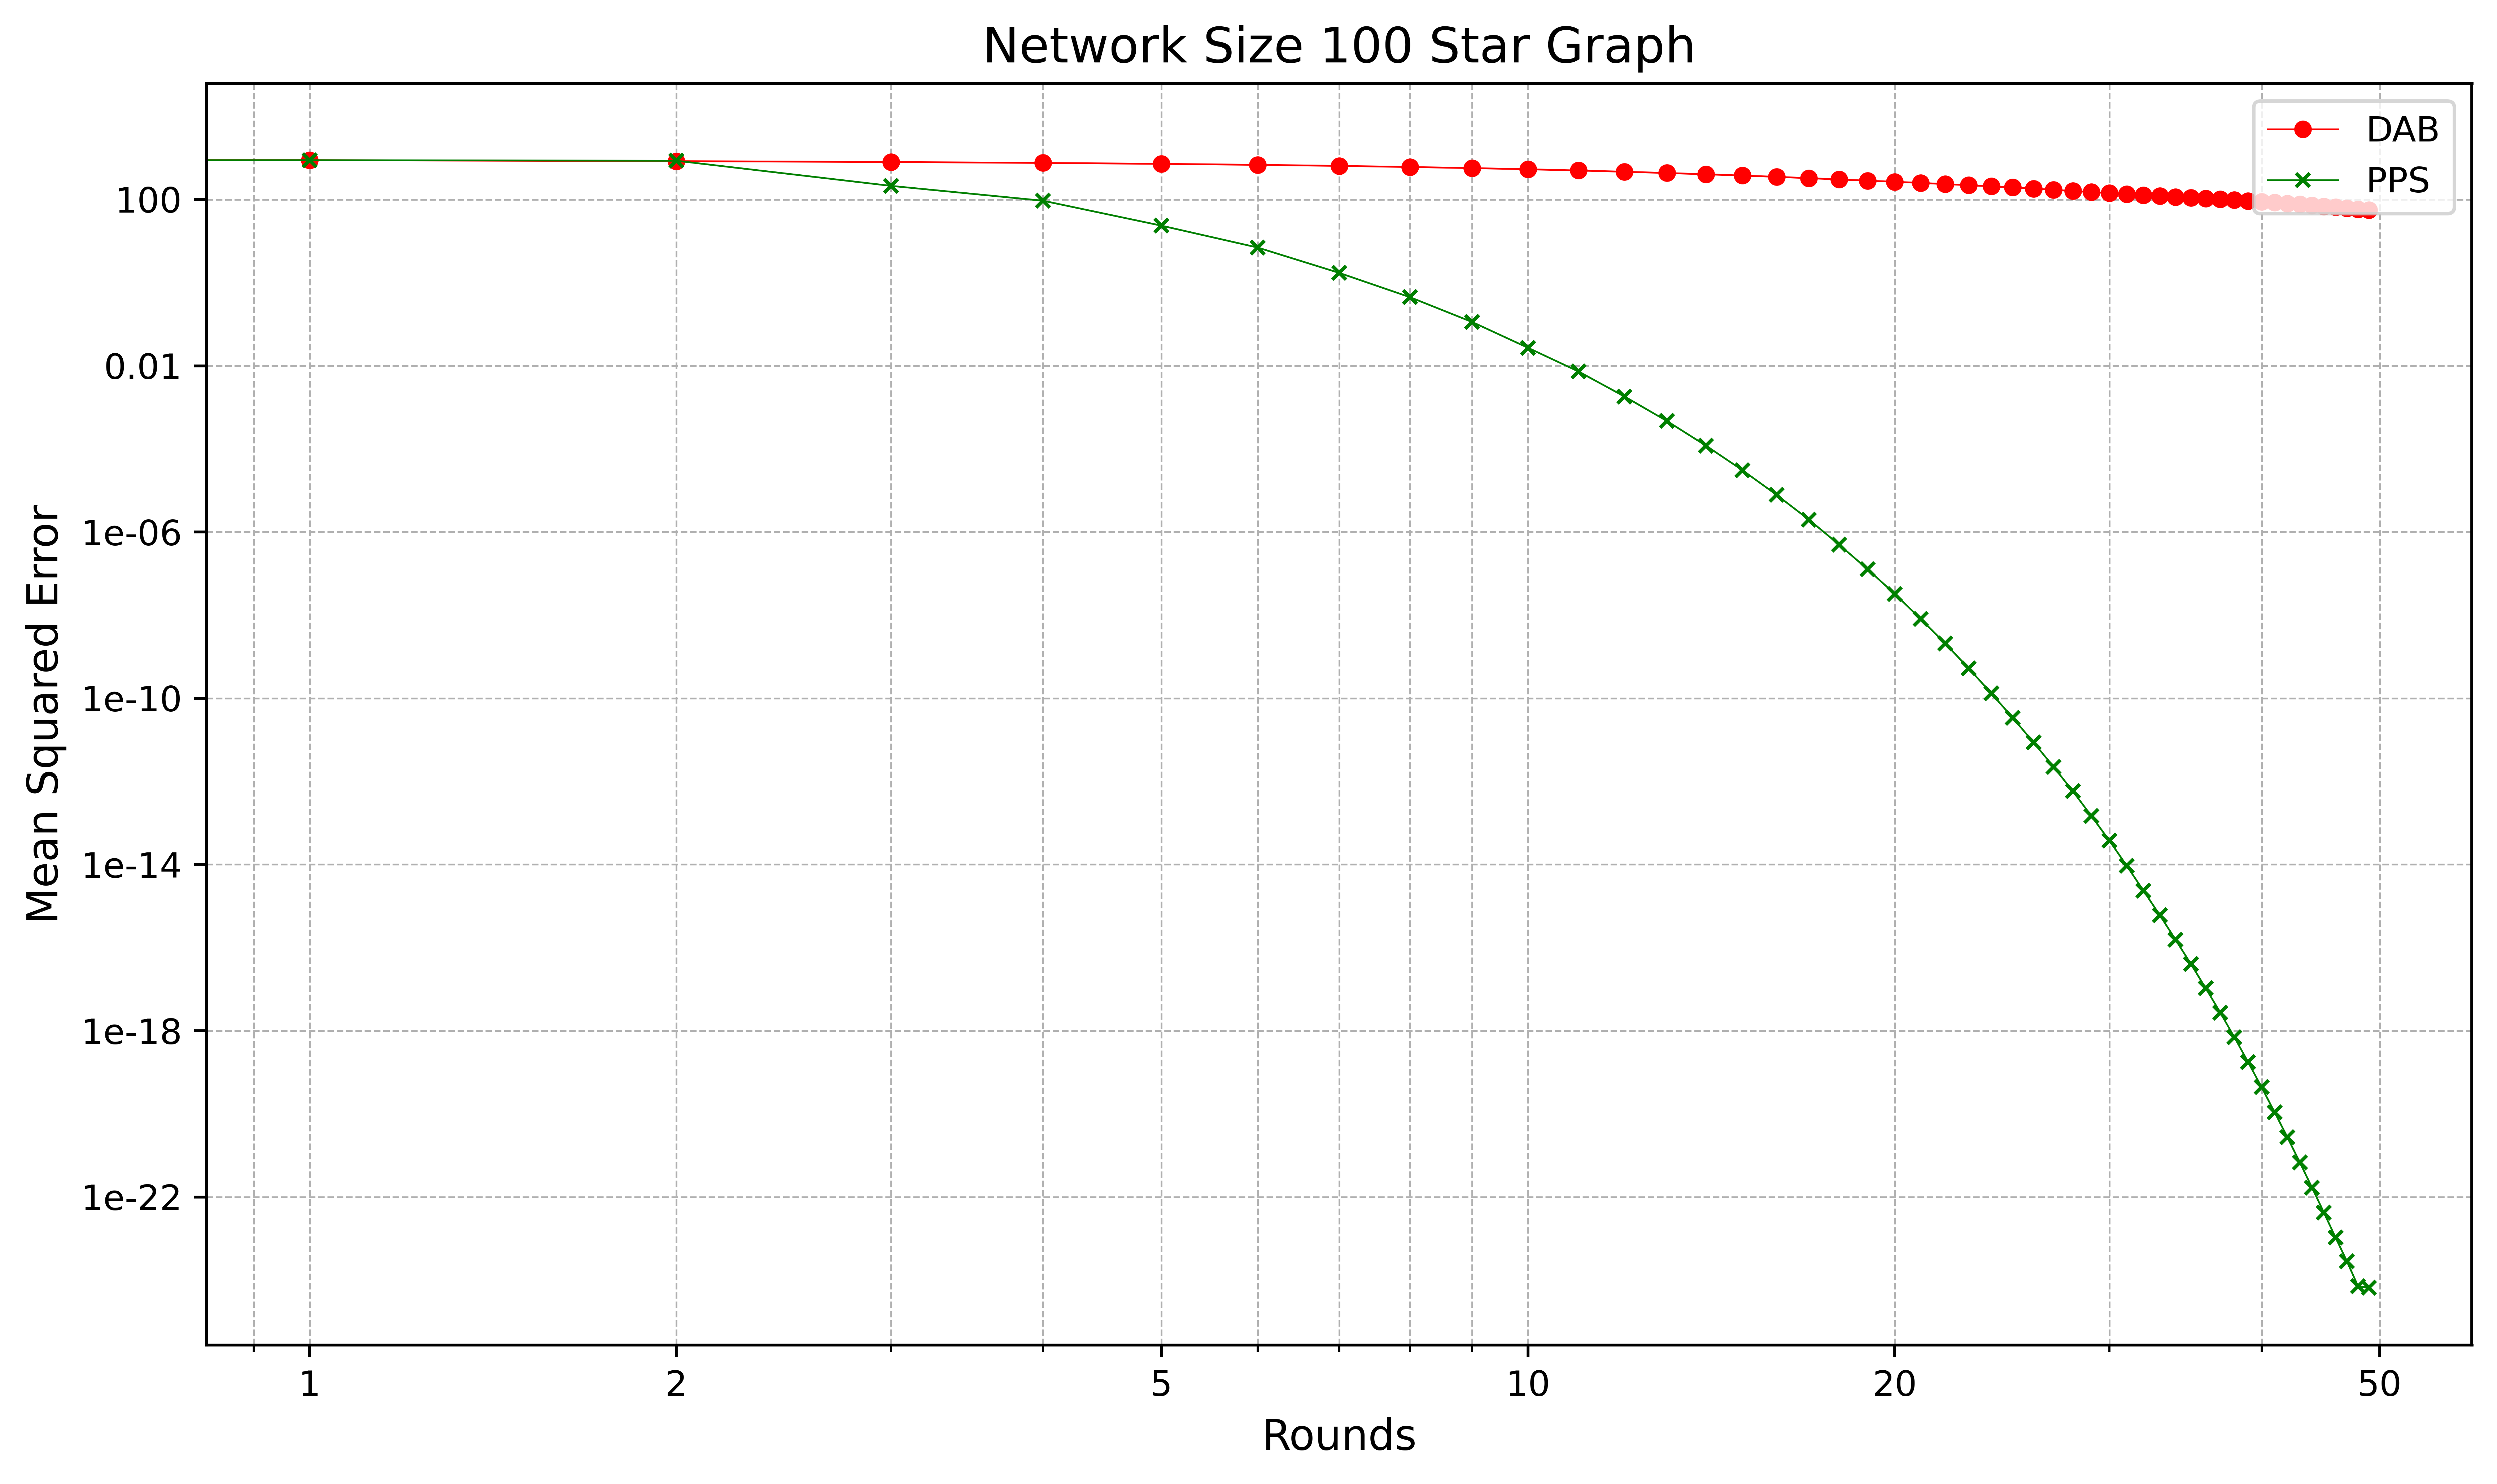
\includegraphics[scale=0.5]{figures/starGraphSimulations/DAB_vs_PPS_SG_r50_n100.png}
    \caption{Star graph: network size $10^{2}$ nodes}
    \label{fig:100StarGraph}
\end{figure}
\begin{figure}[H]
    \centering
    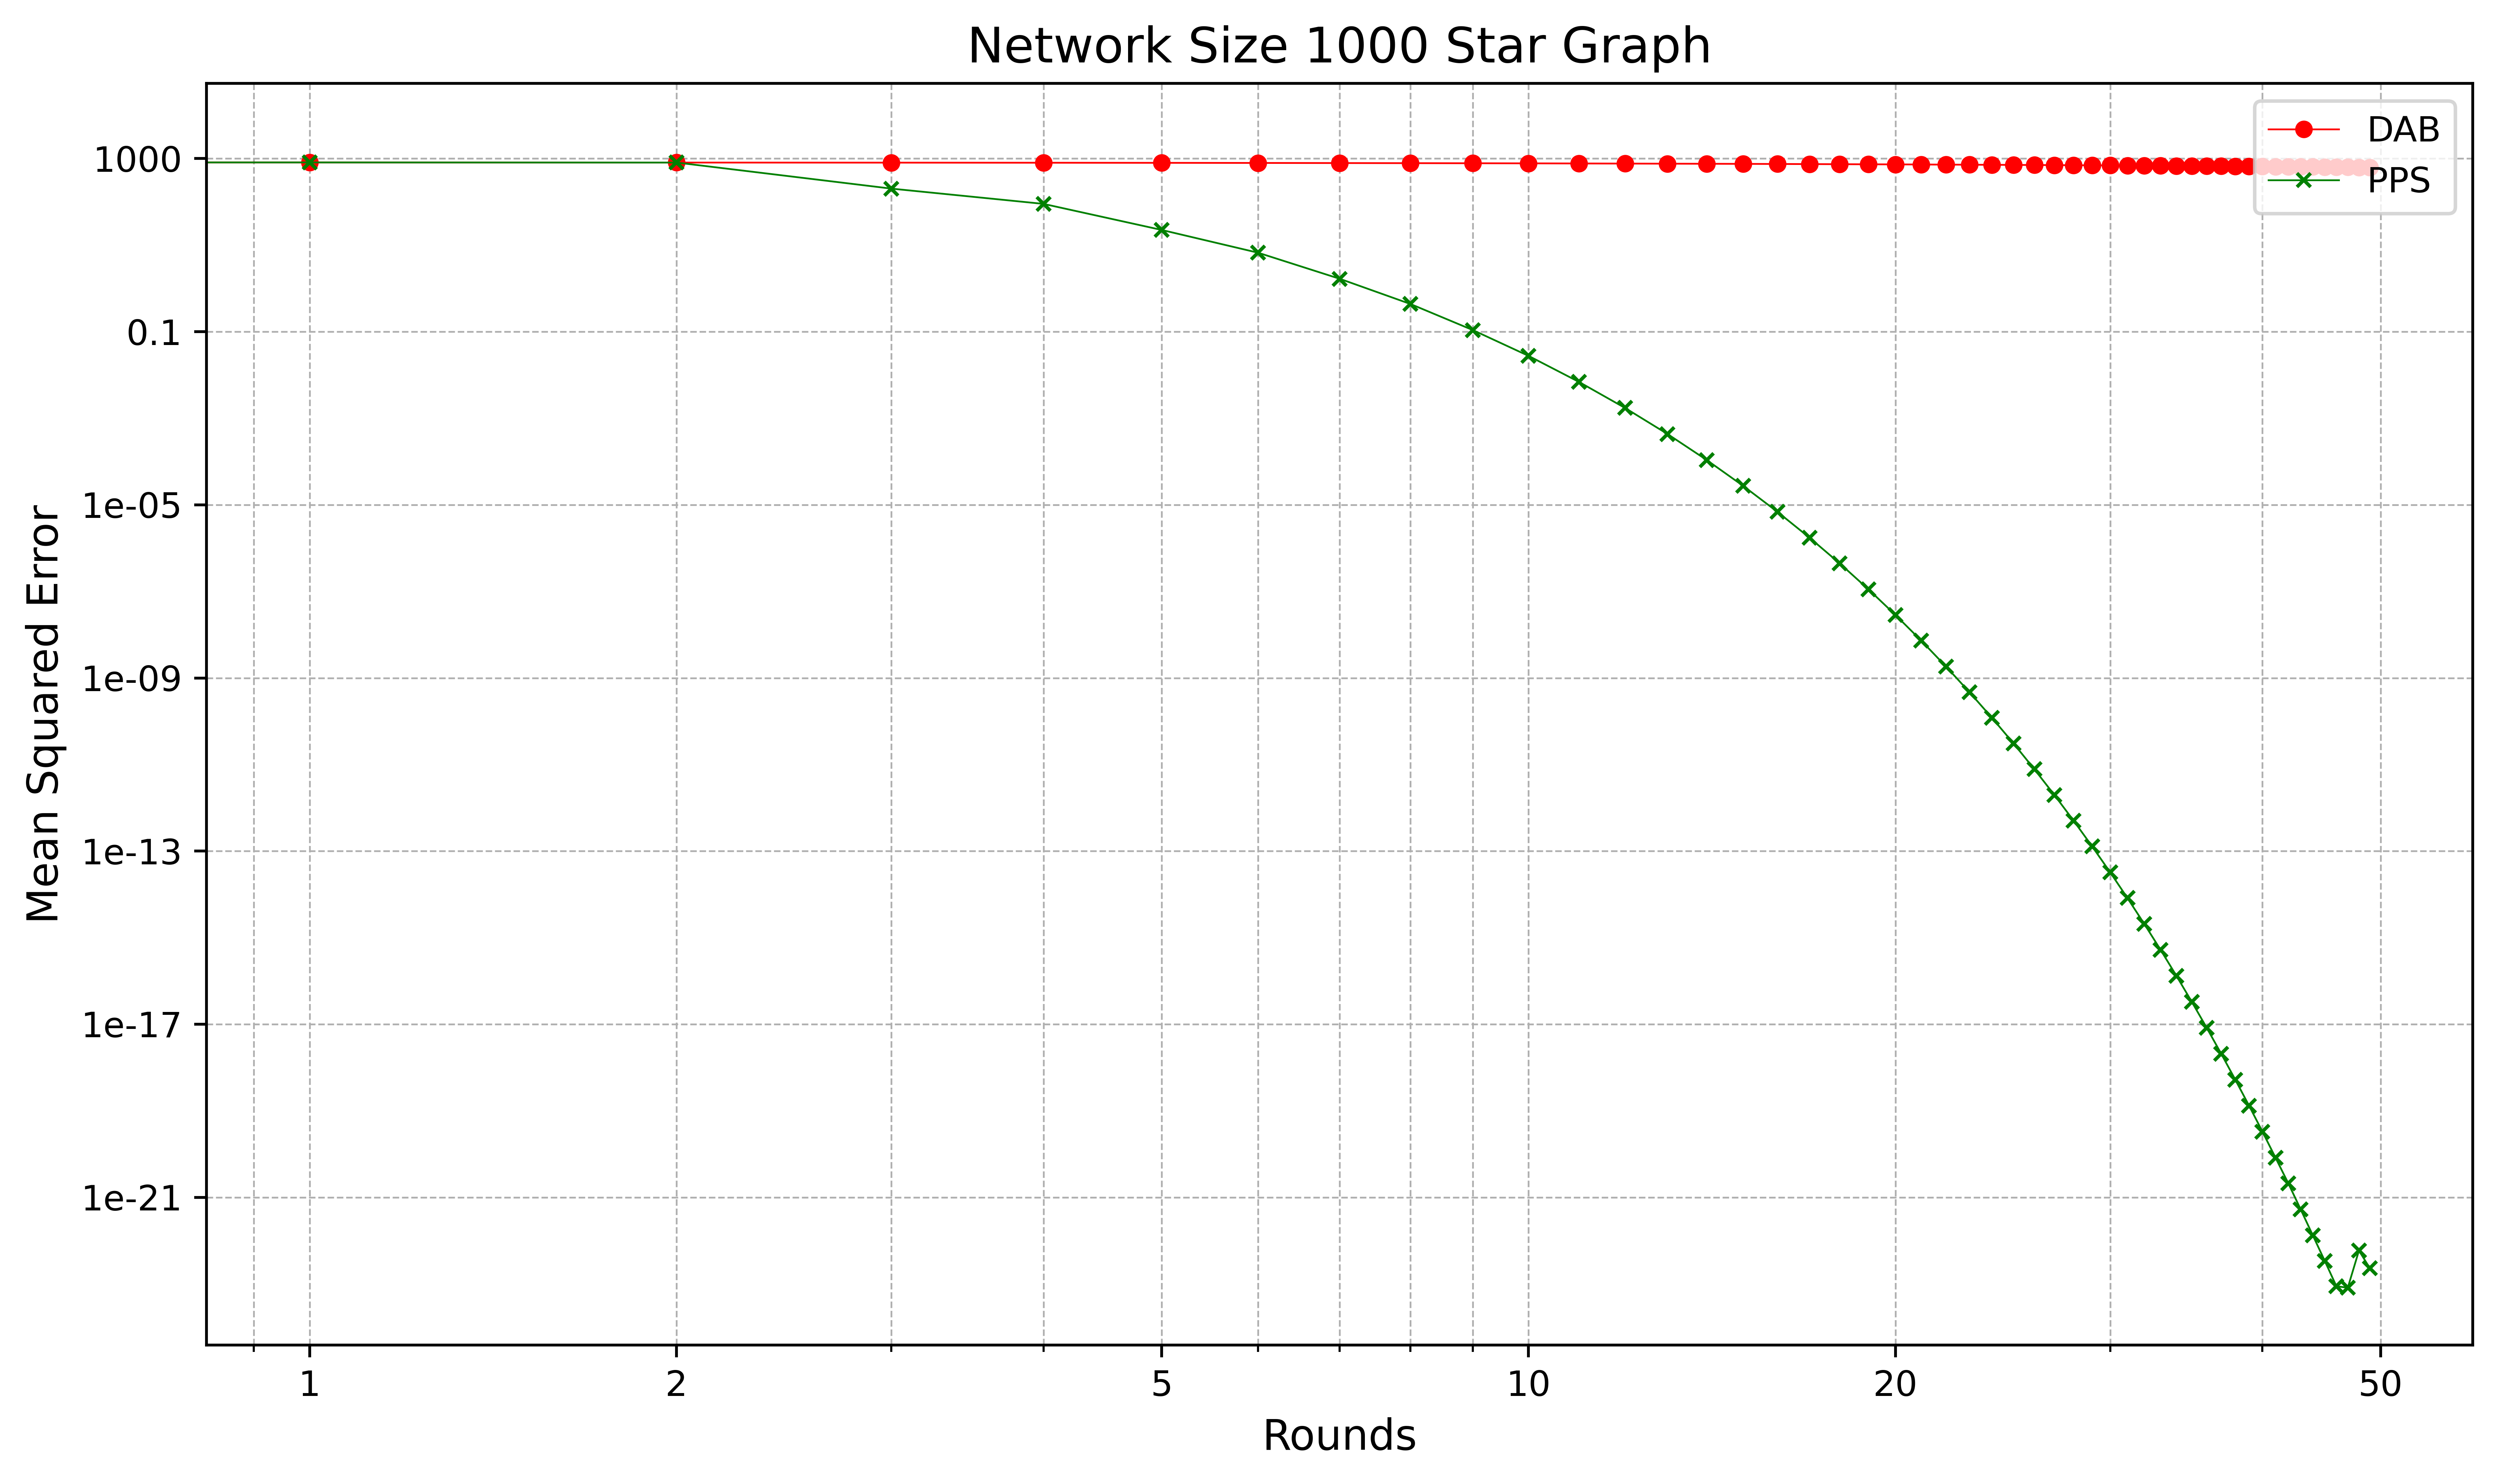
\includegraphics[scale=0.5]{figures/starGraphSimulations/DAB_vs_PPS_SG_r50_n1000.png}
    \caption{Star graph: network size $10^{3}$ nodes}
    \label{fig:1000StarGraph}
\end{figure}
\begin{figure}[H]
    \centering
    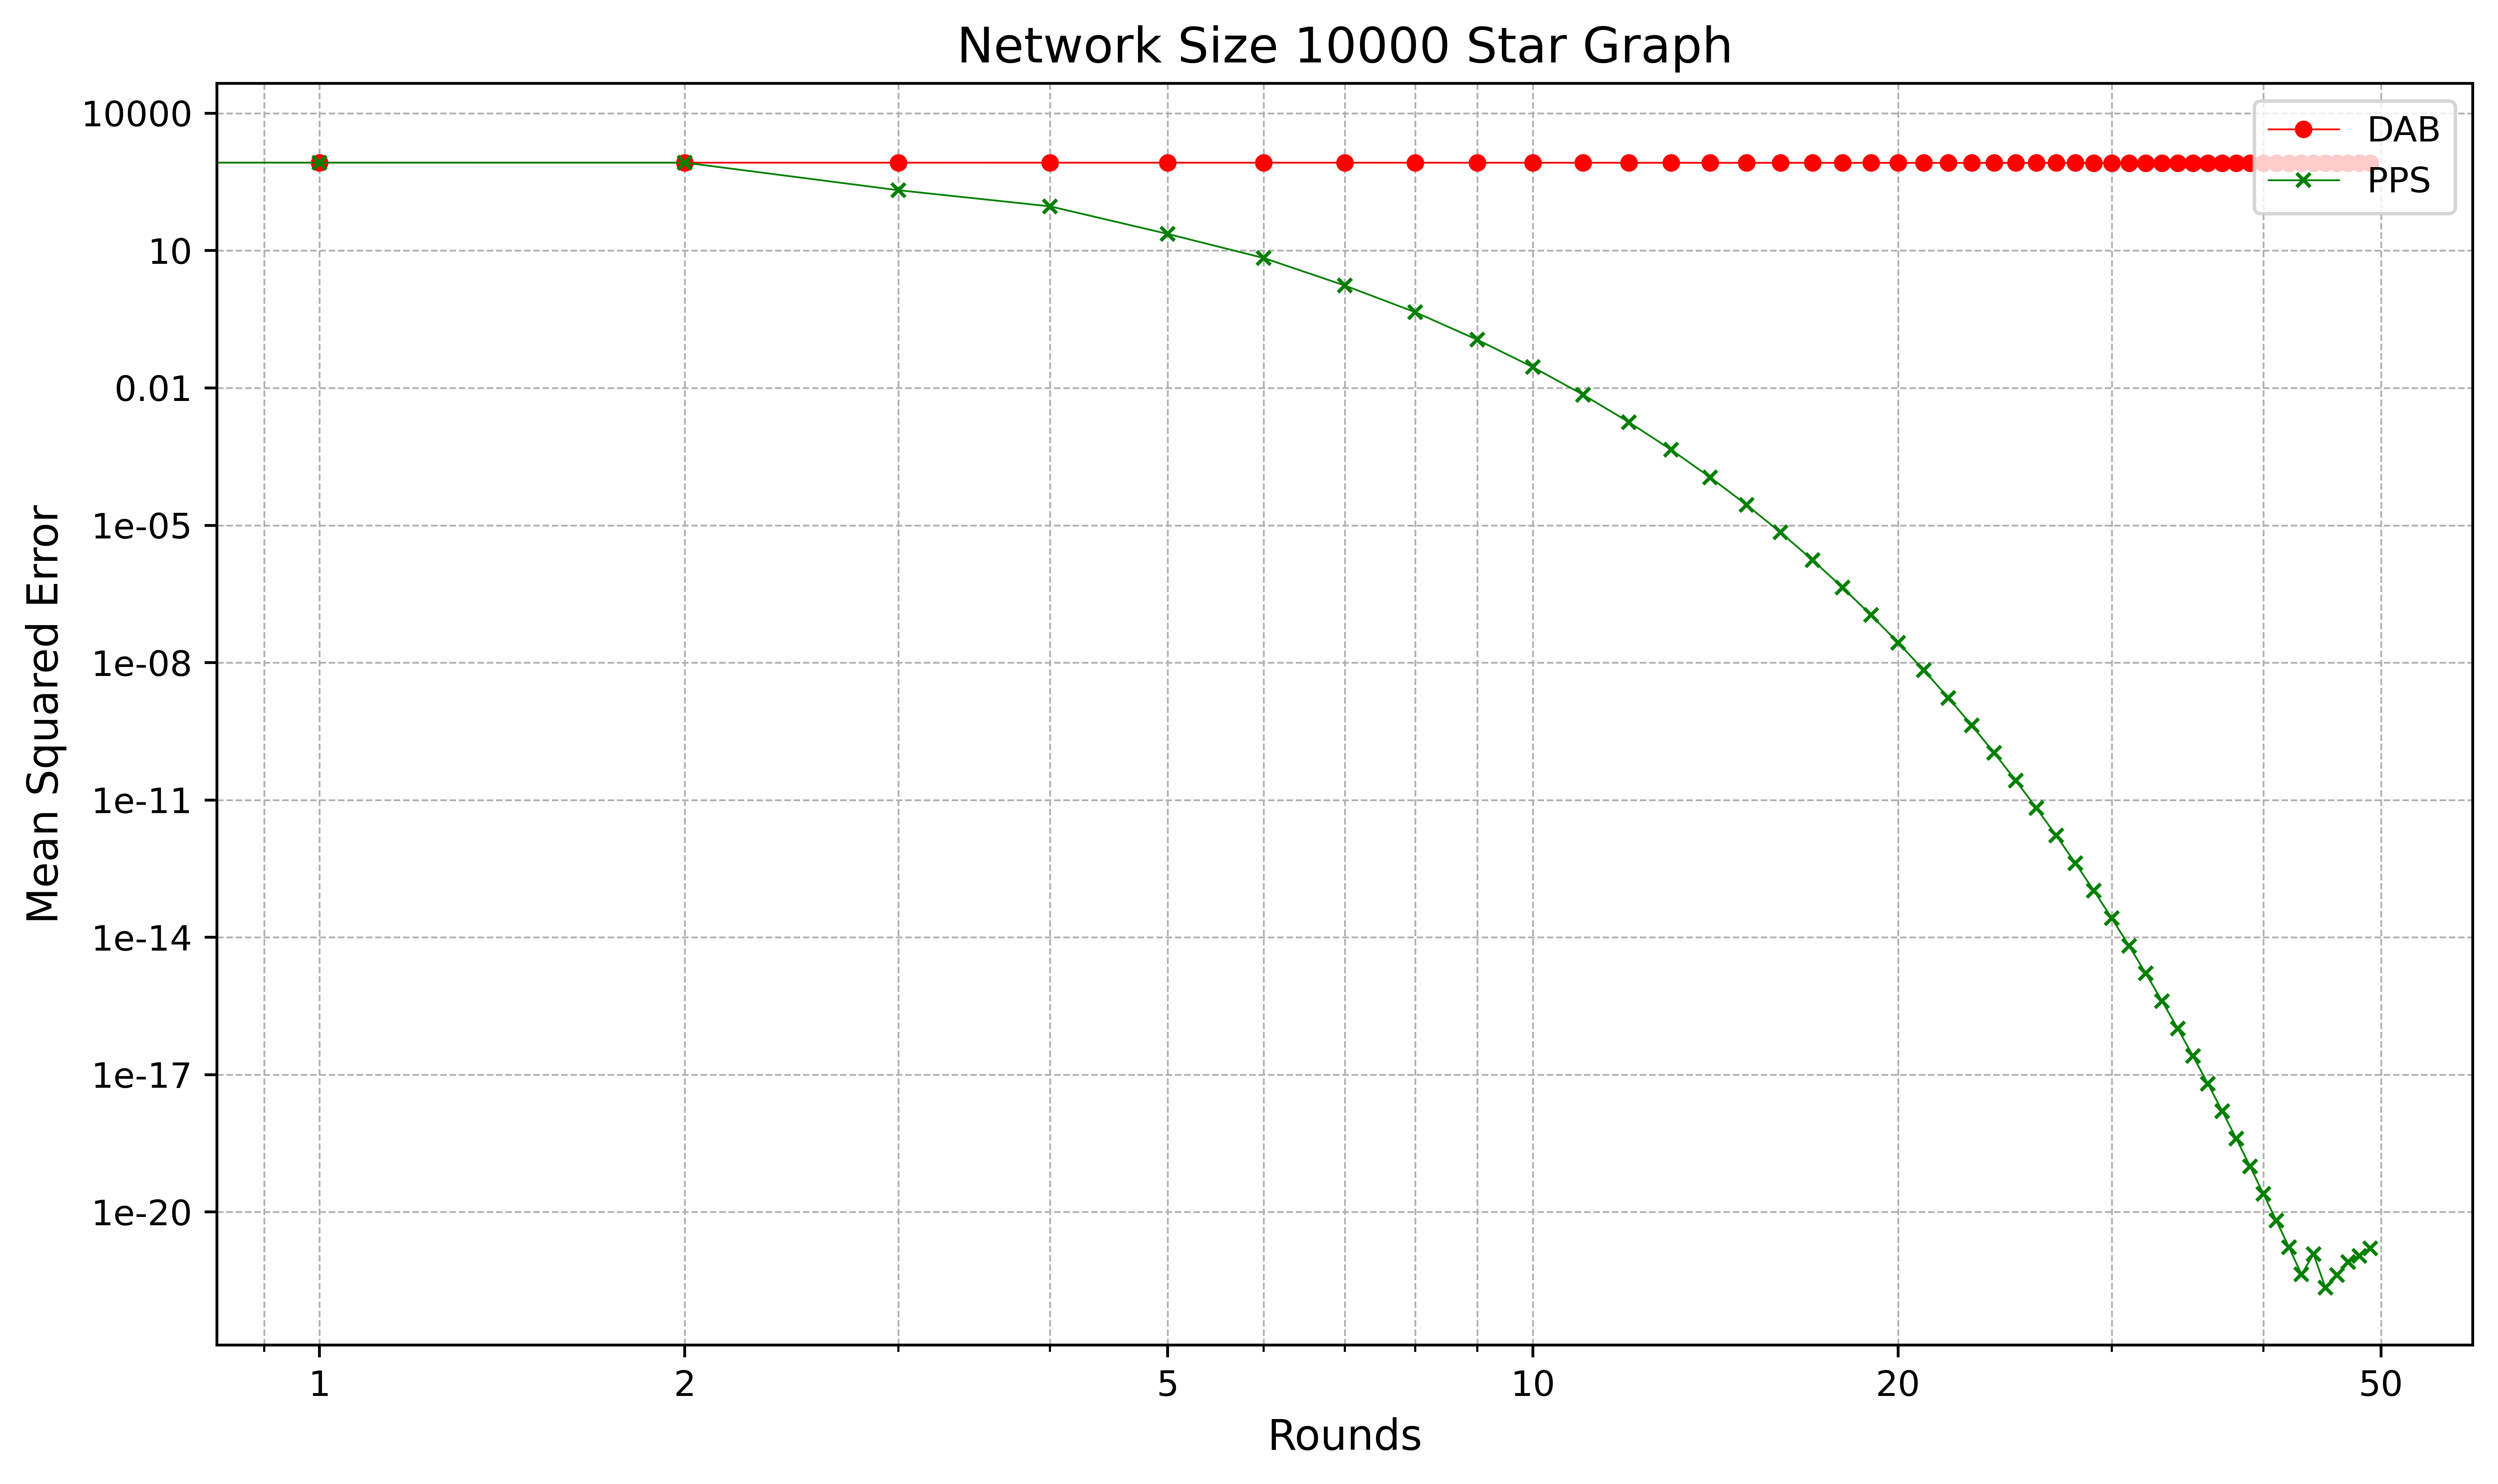
\includegraphics[scale=0.5]{figures/starGraphSimulations/DAB_vs_PPS_SG_r50_n10000.png}
    \caption{Star graph: network size $10^{4}$ nodes}
    \label{fig:10000StarGraph}
\end{figure}

\subsection{Closed Chain Graph}
\begin{figure}[H]
    \centering
    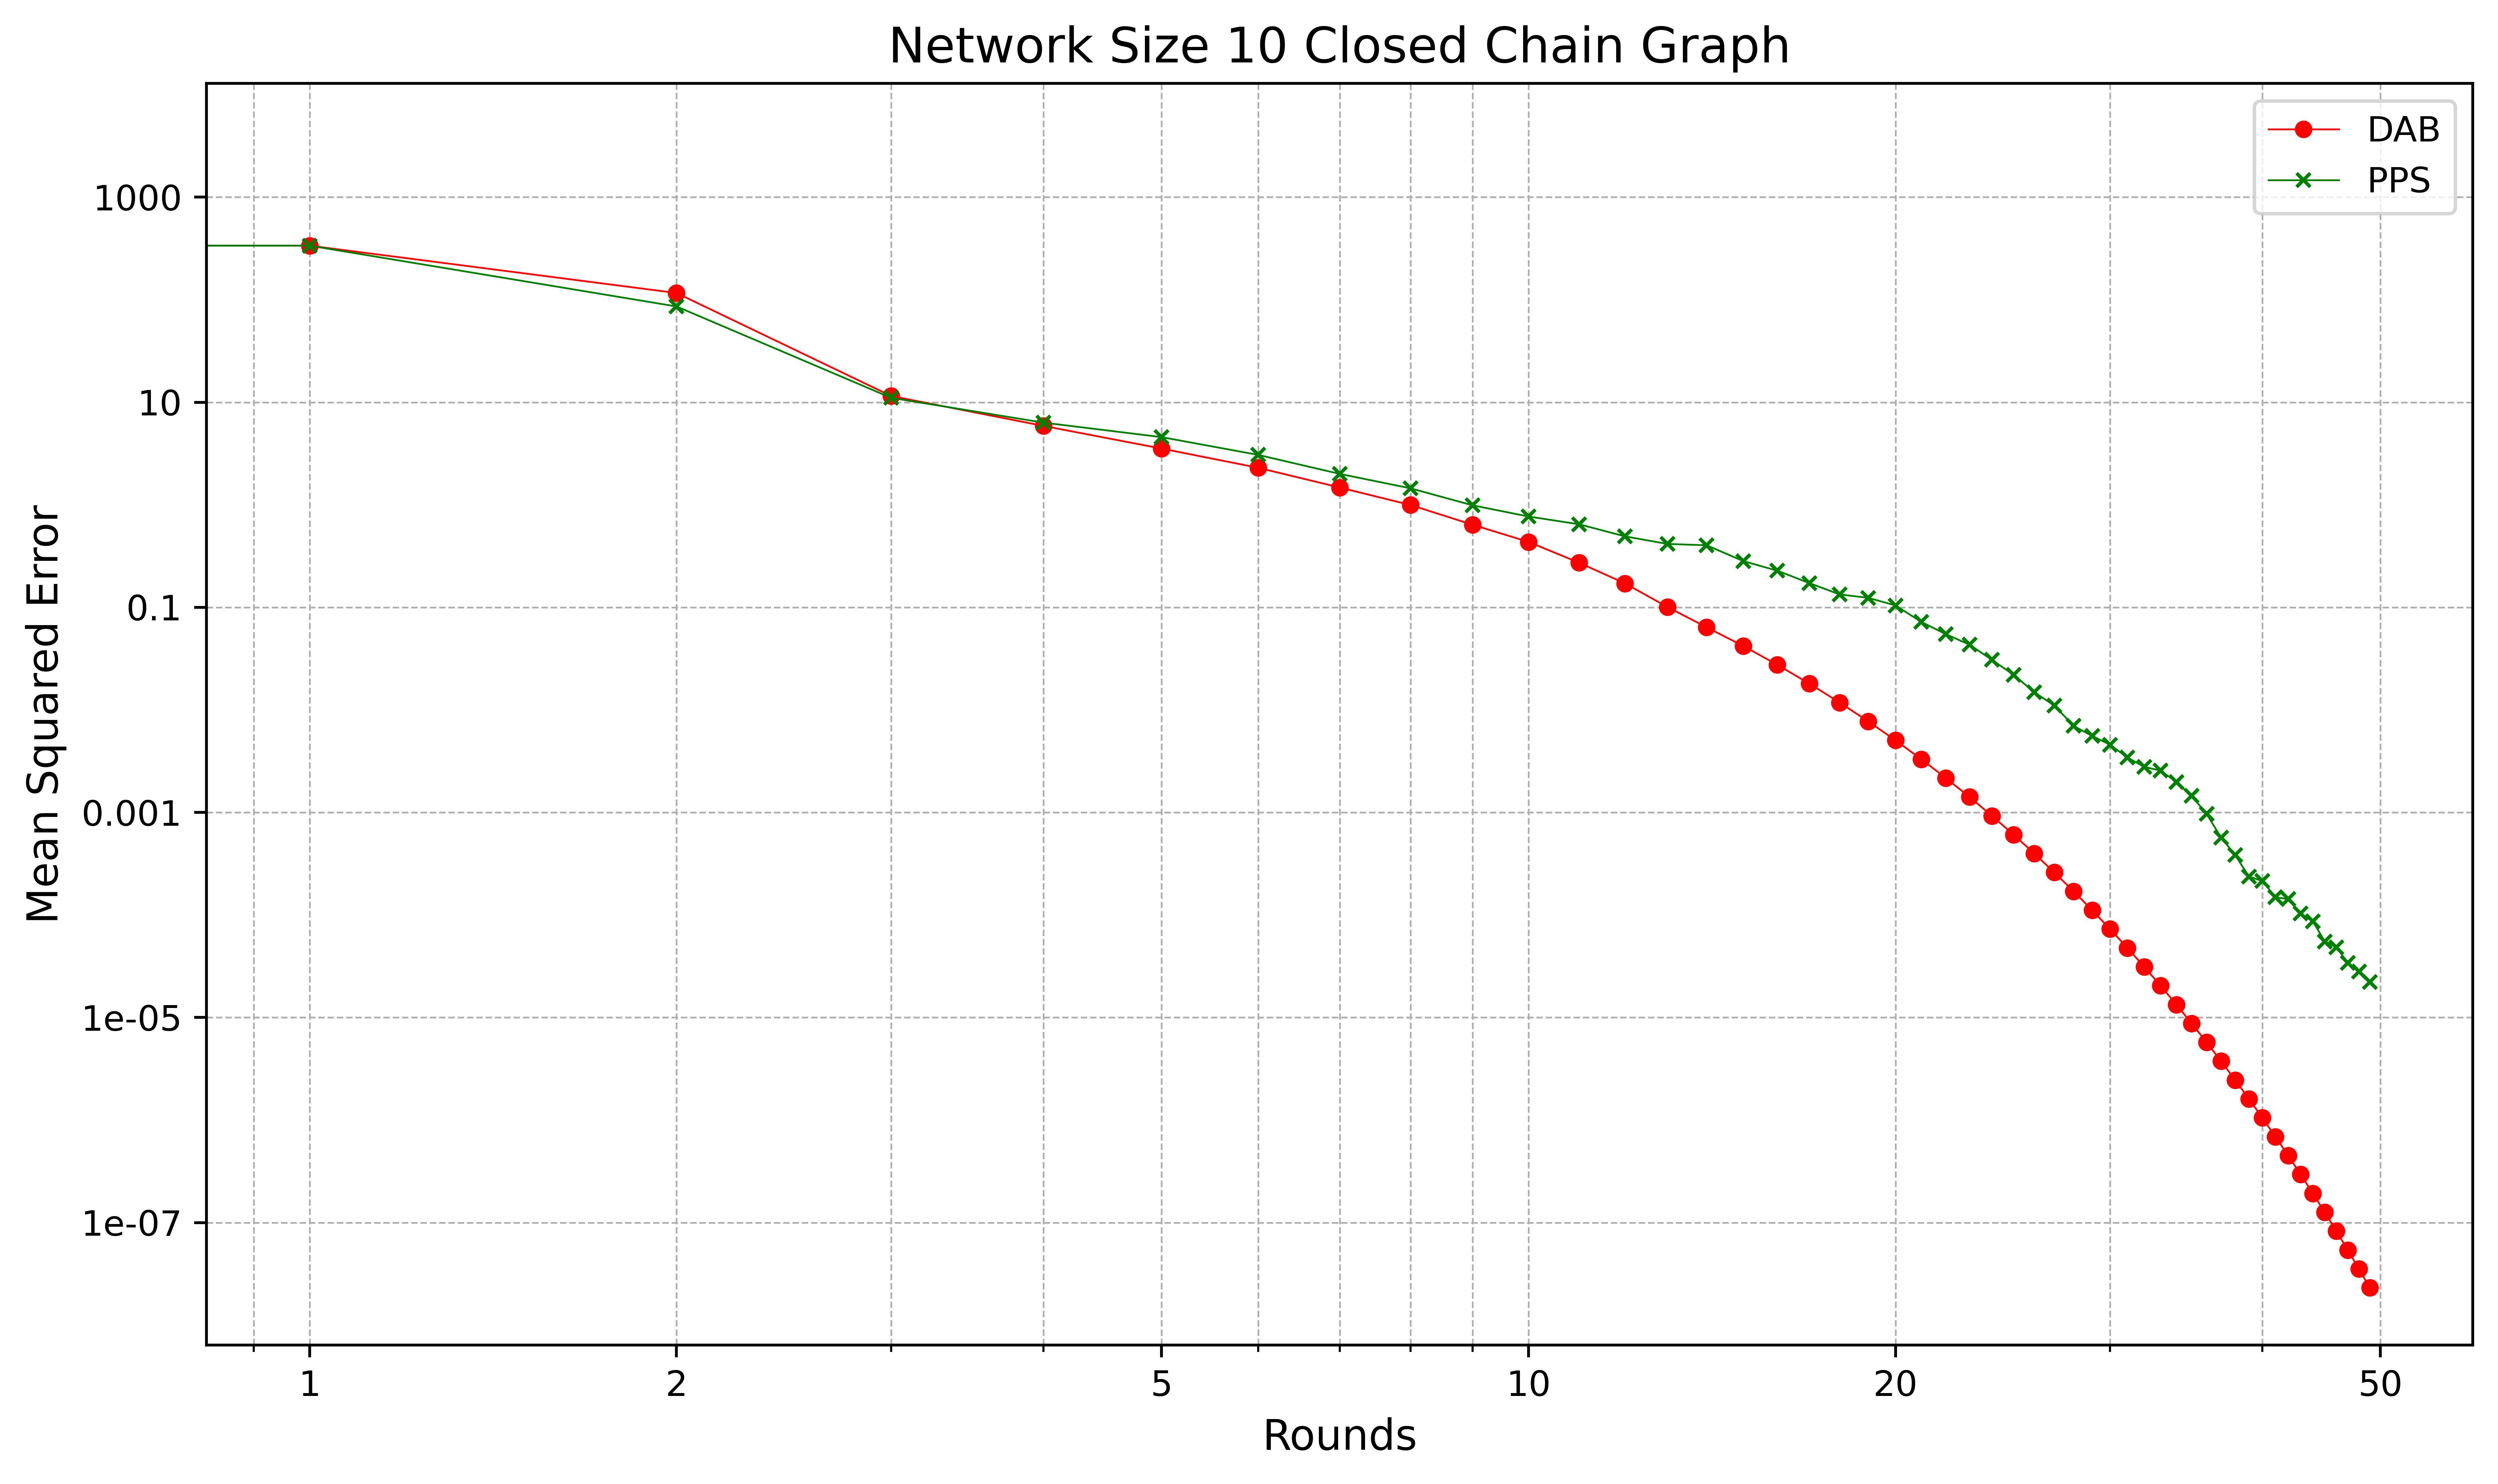
\includegraphics[scale=0.5]{figures/closedChainSimulations/DAB_vs_PPS_CCG_r50_n10.png}
    \caption{Closed chain graph: network size $10^{1}$ nodes}
    \label{fig:10ChainGraph}
\end{figure}
\begin{figure}[H]
    \centering
    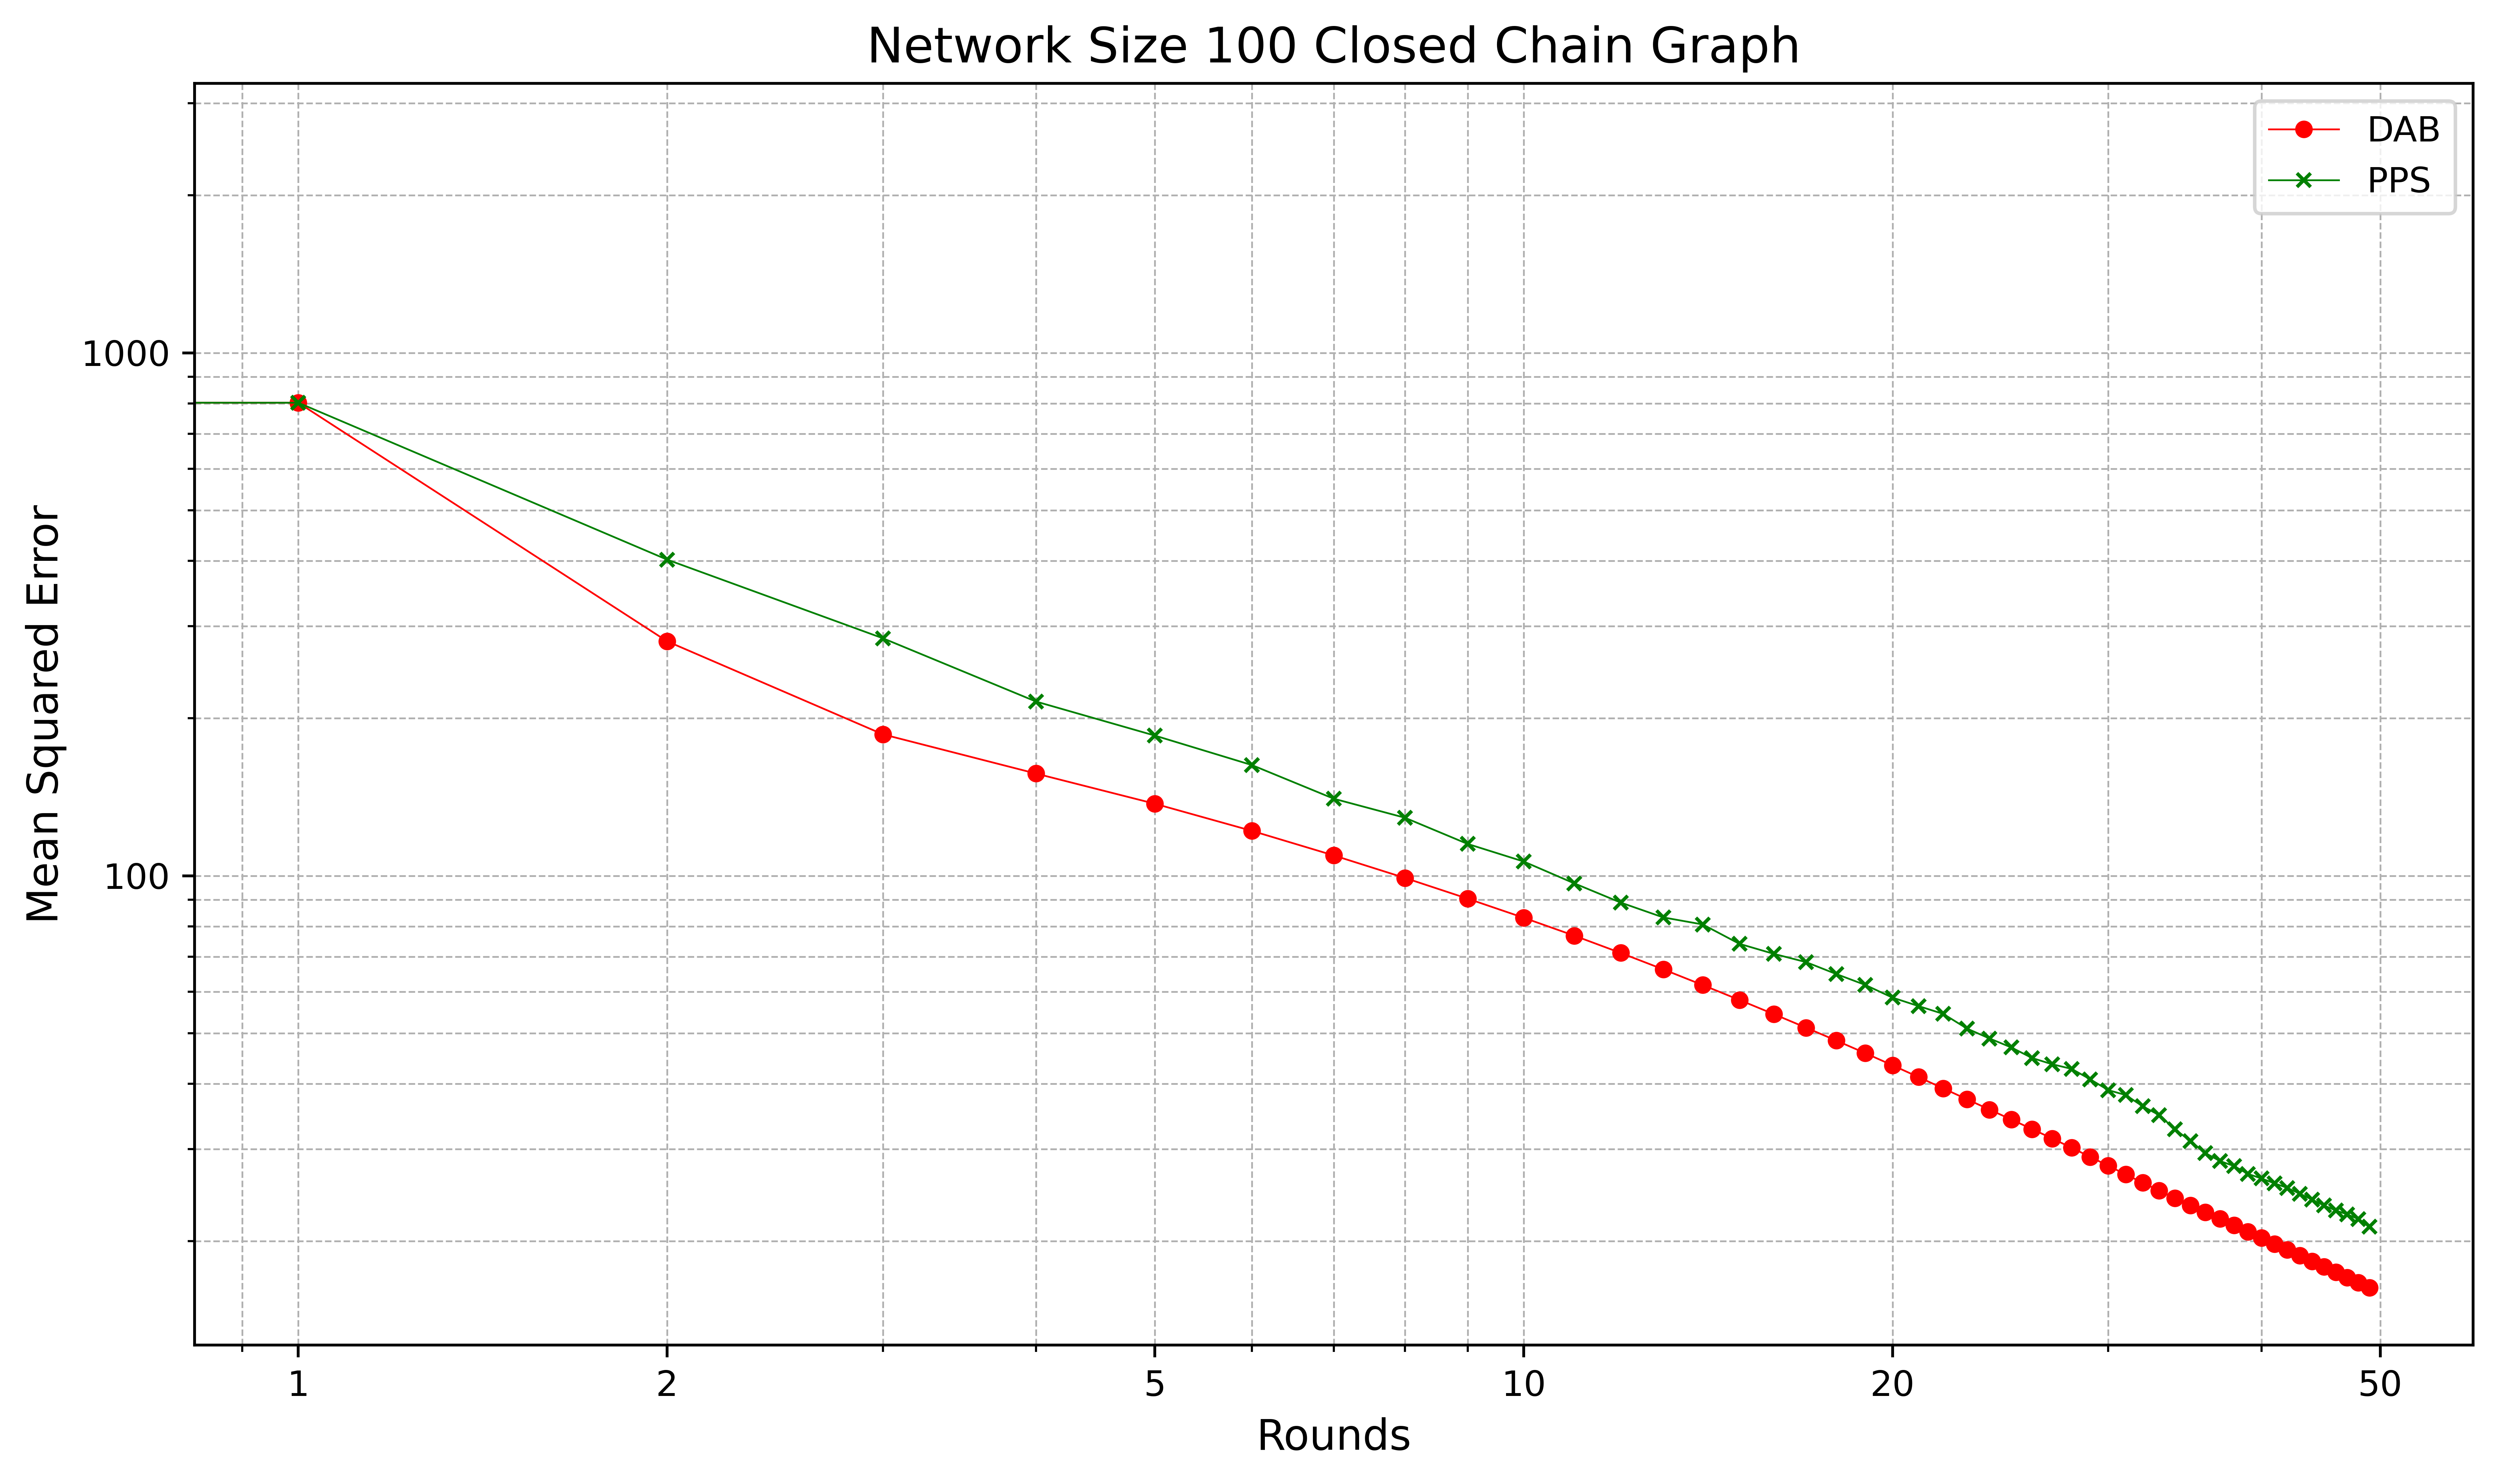
\includegraphics[scale=0.5]{figures/closedChainSimulations/DAB_vs_PPS_CCG_r50_n100.png}
    \caption{Closed chain graph: network size $10^{2}$ nodes}
    \label{fig:100ChainGraph}
\end{figure}
\begin{figure}[H]
    \centering
    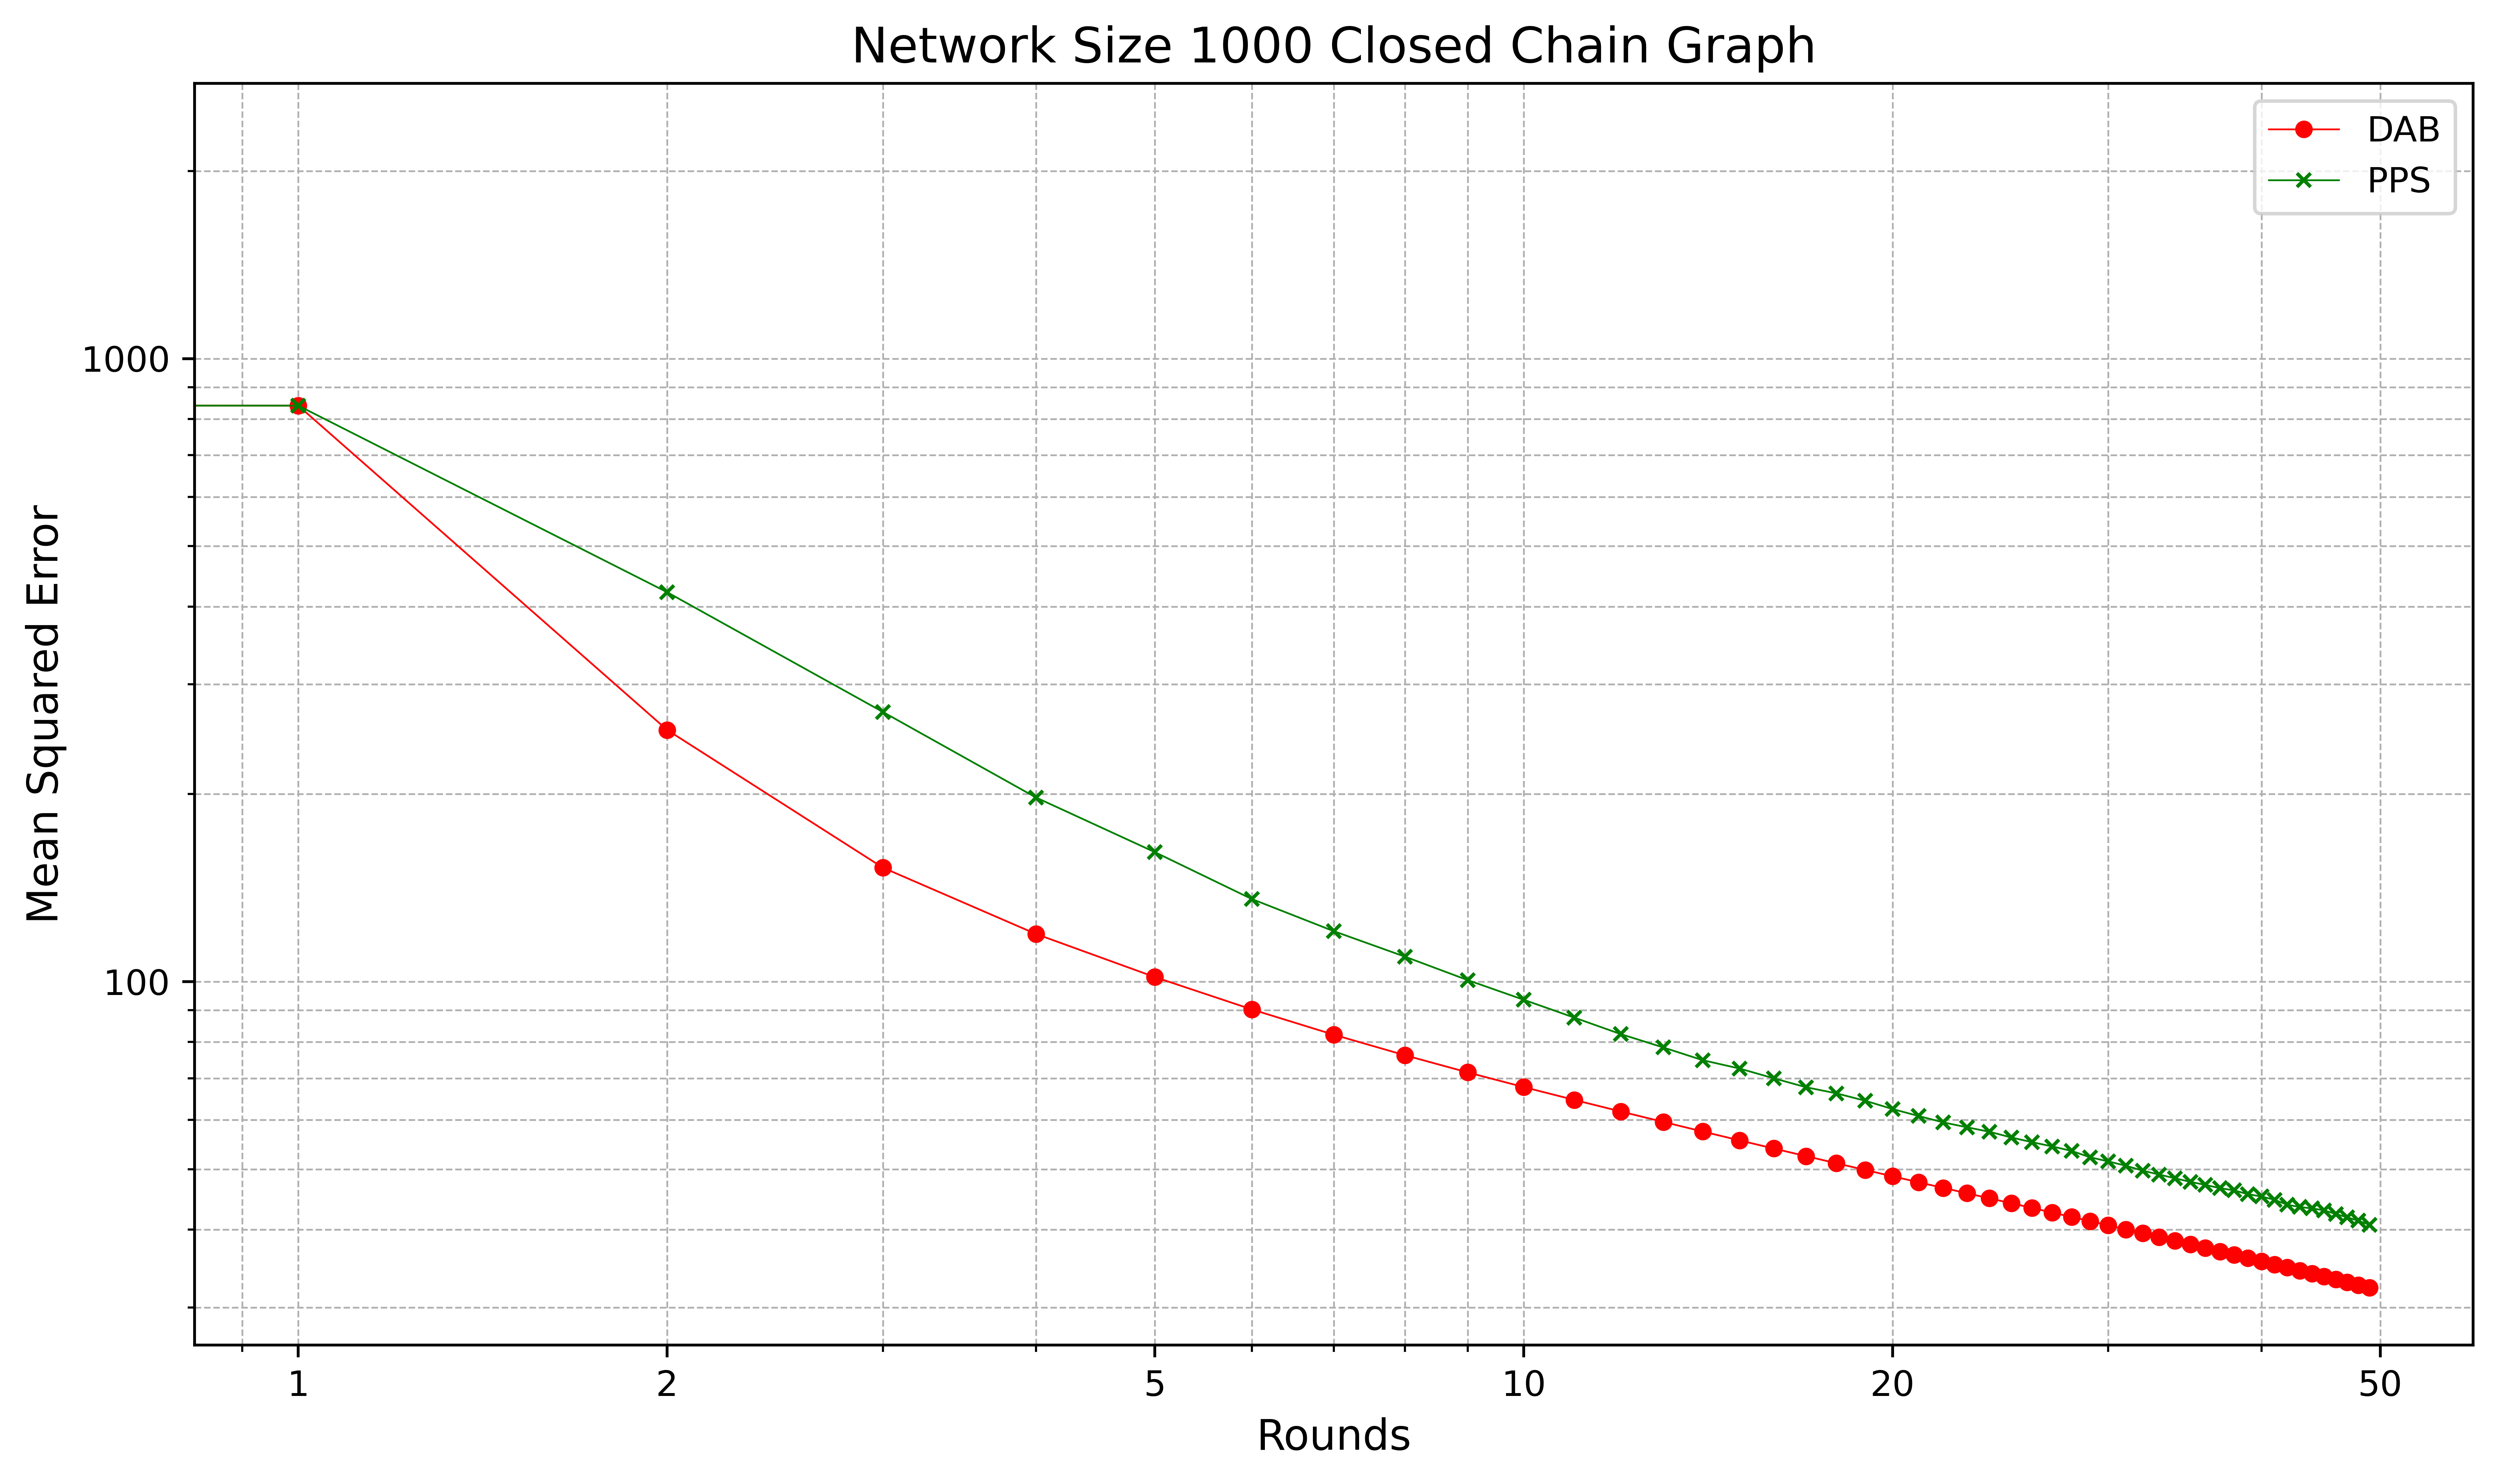
\includegraphics[scale=0.5]{figures/closedChainSimulations/DAB_vs_PPS_CCG_r50_n1000.png}
    \caption{Closed chain graph: network size $10^{3}$ nodes}
    \label{fig:1000ChainGraph}
\end{figure}
\begin{figure}[H]
    \centering
    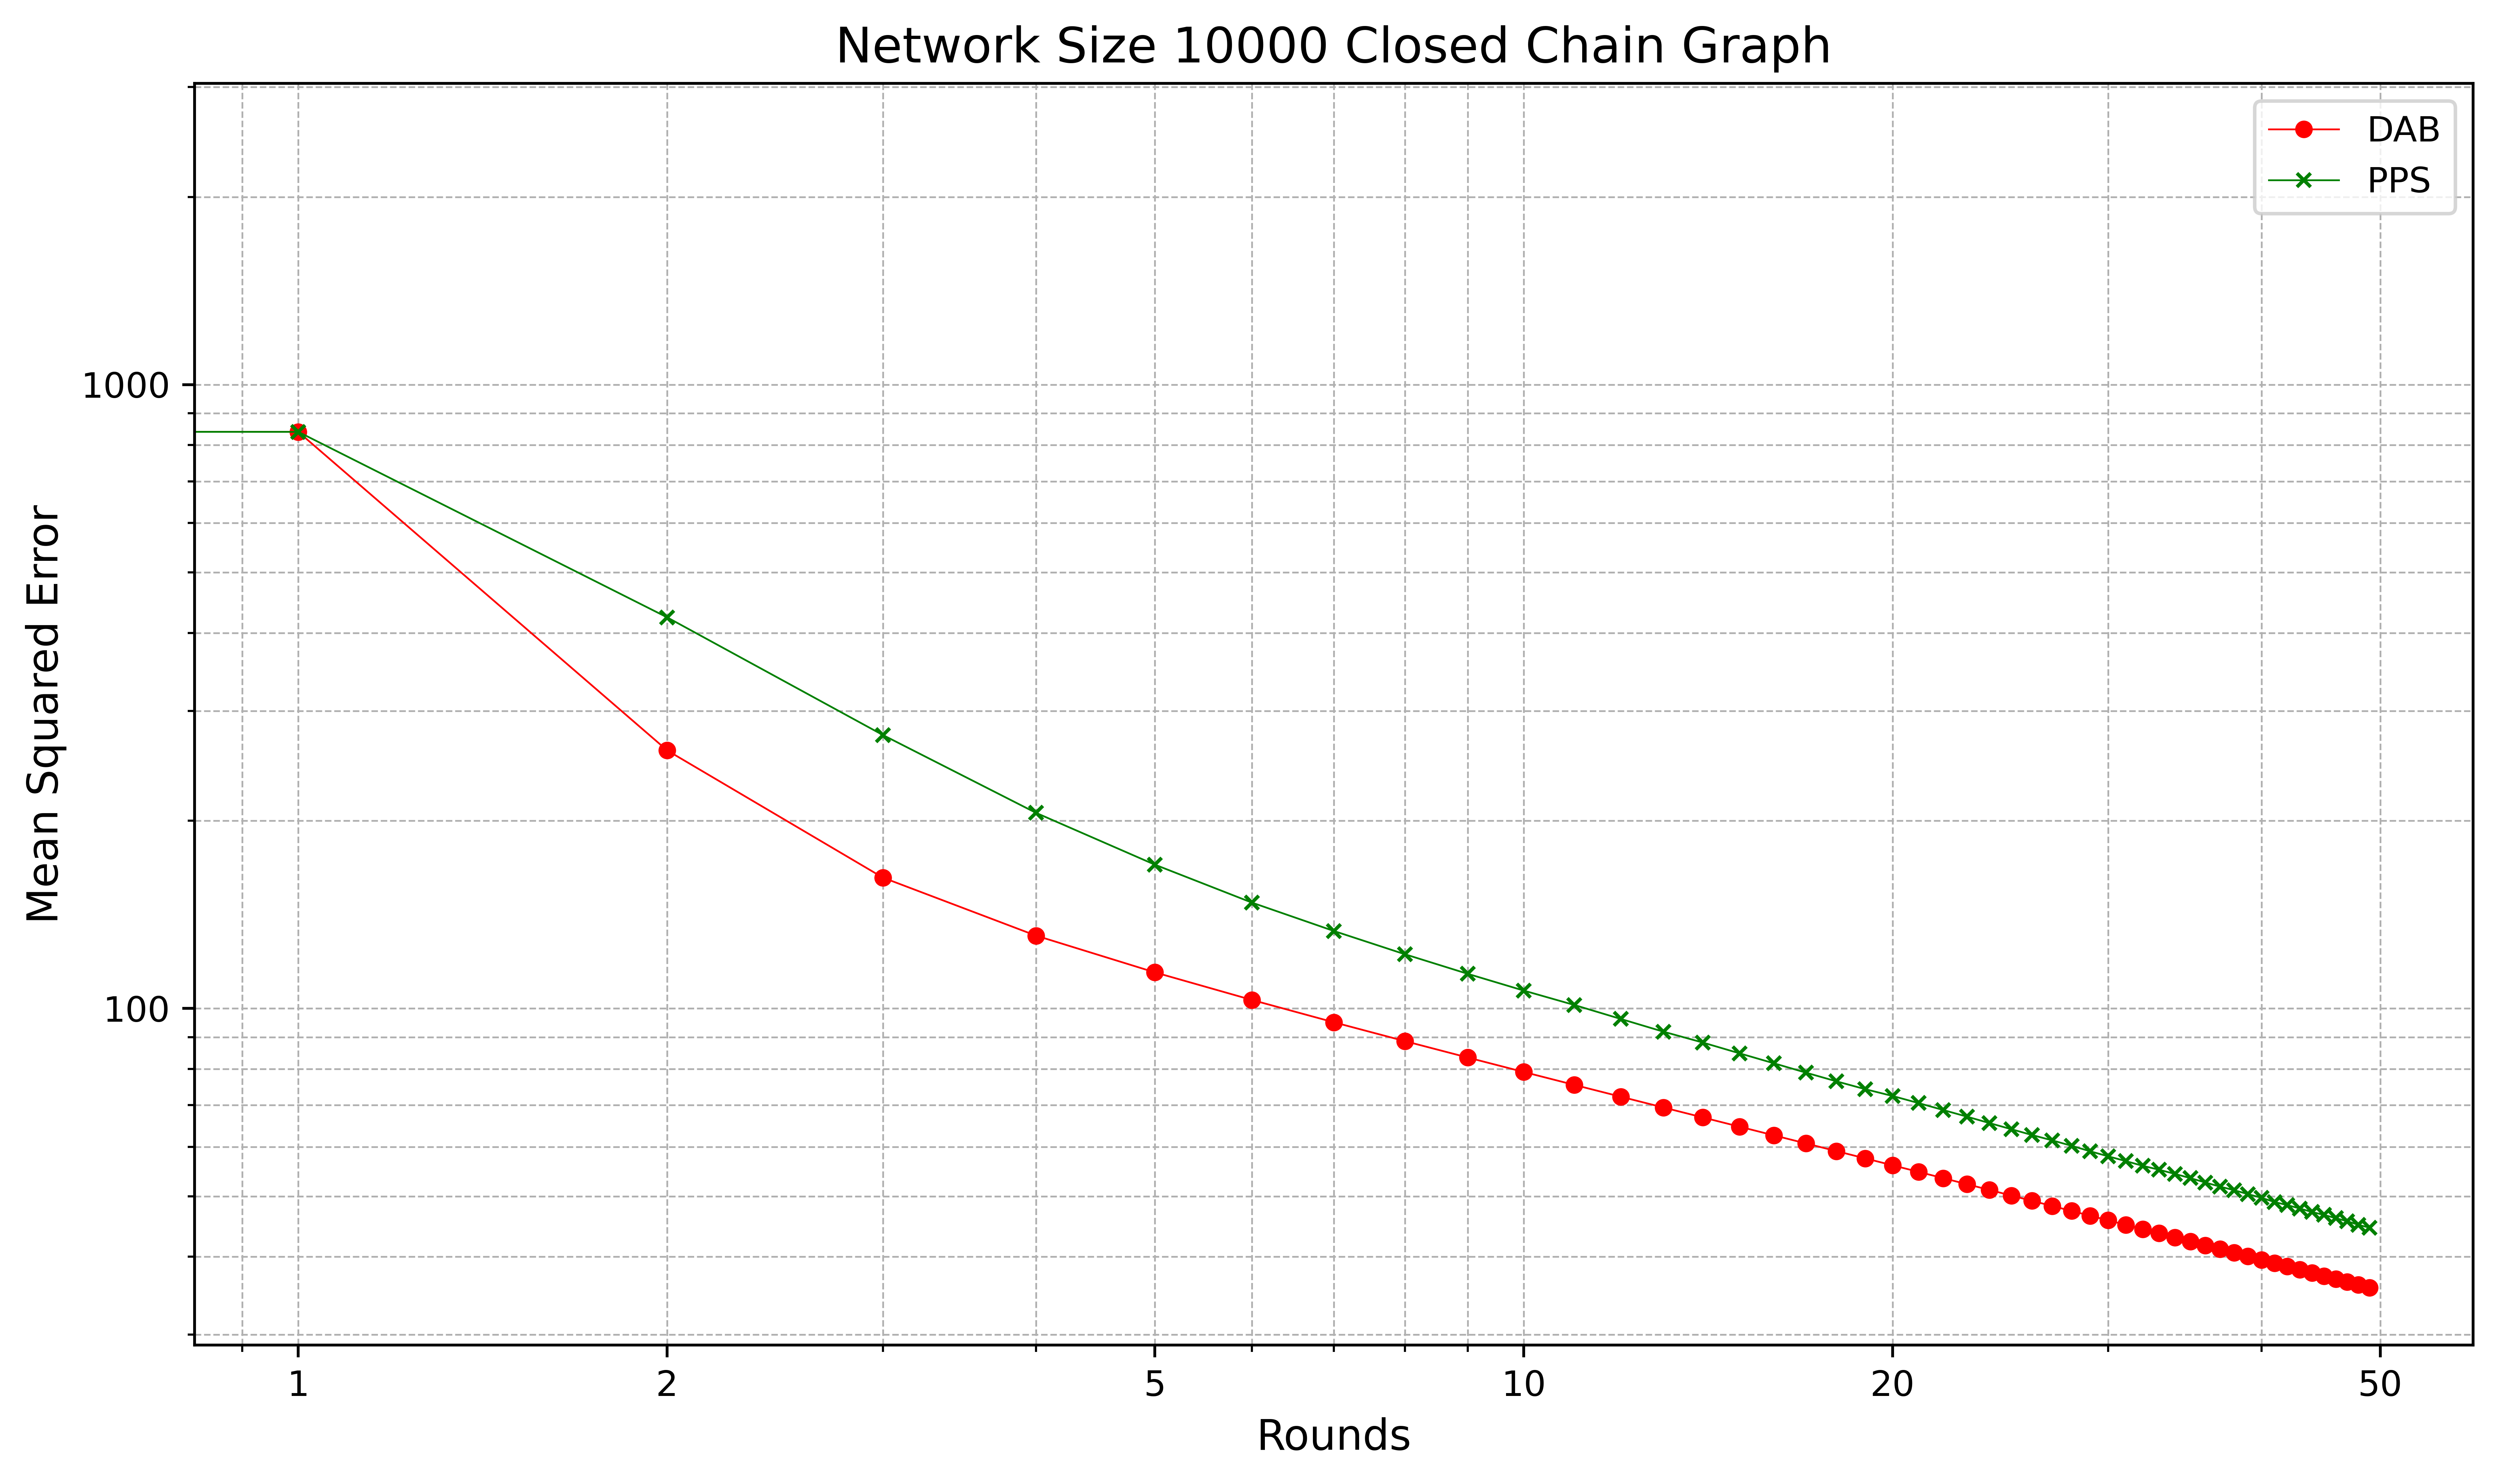
\includegraphics[scale=0.5]{figures/closedChainSimulations/DAB_vs_PPS_CCG_r50_n10000.png}
    \caption{Closed chain graph: network size $10^{4}$ nodes}
    \label{fig:10000ChainGraph}
\end{figure}

\subsection{Torus Grid Graph}
\begin{figure}[H]
    \centering
    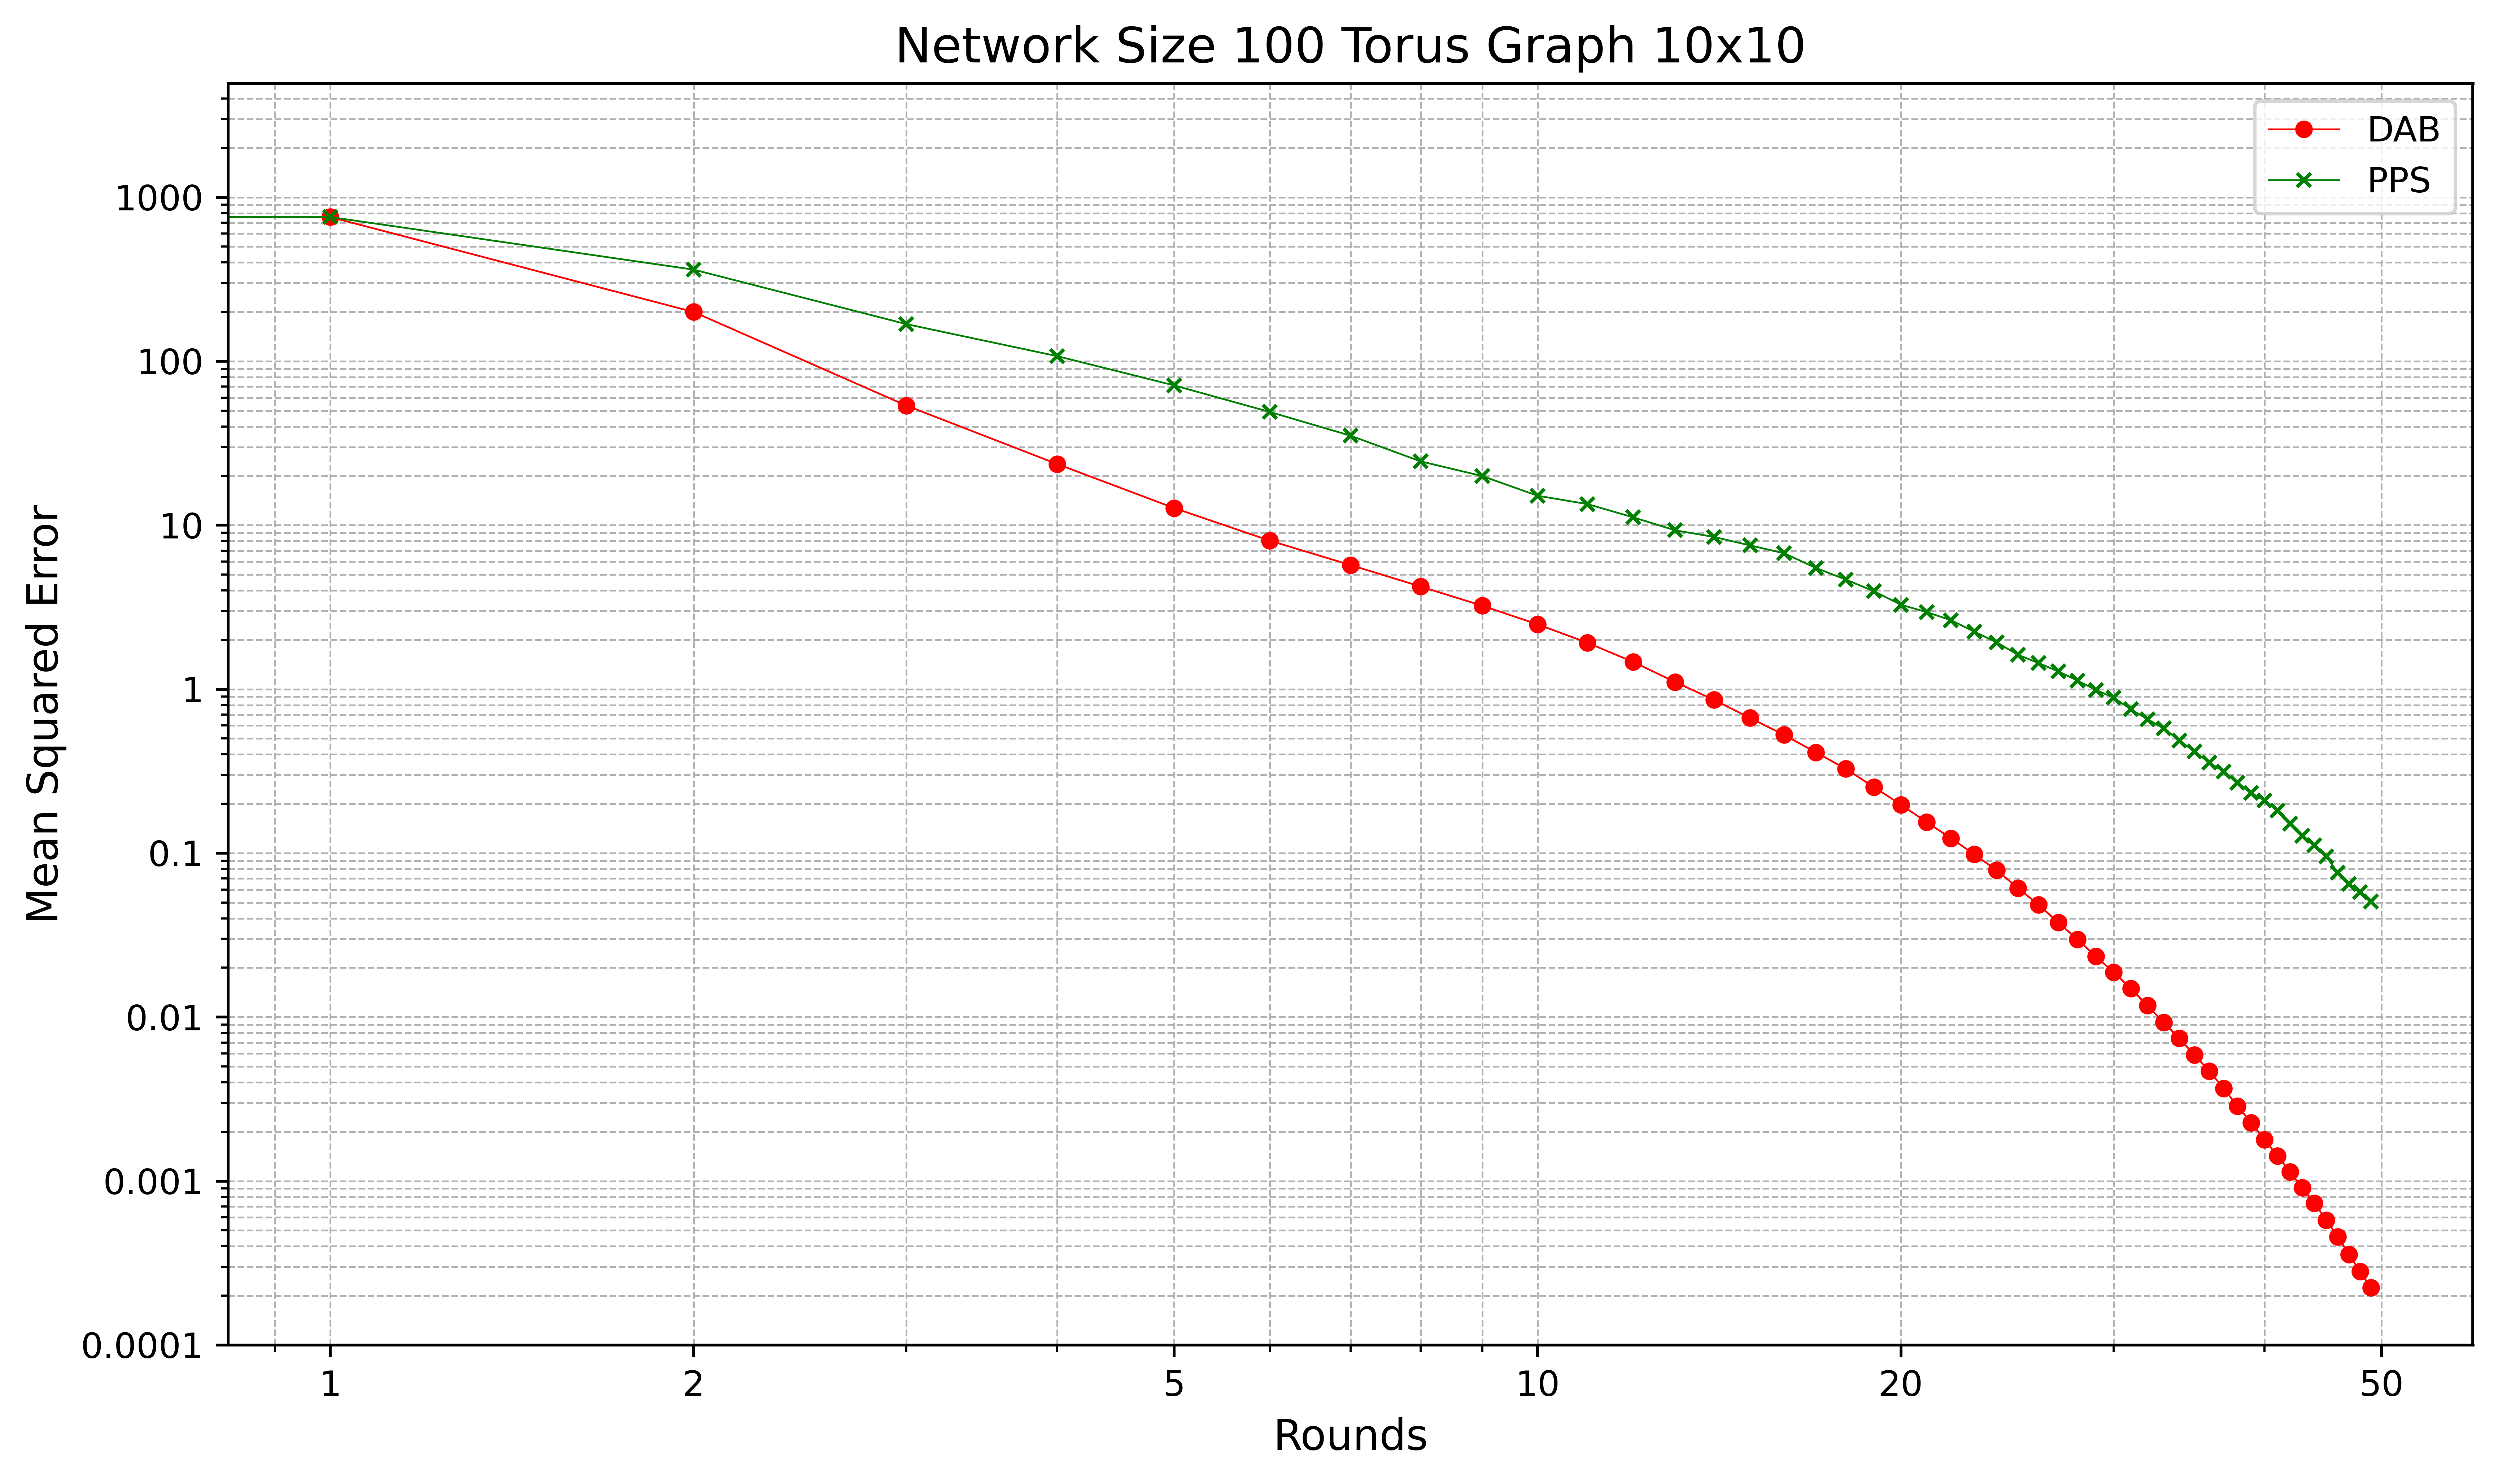
\includegraphics[scale=0.5]{figures/torusGridGraphSimulations/DAB_vs_PPS_TG_r50_n100.png}
    \caption{Torus grid graph: network size $10^{2}$ nodes $(10 \times 10)$}
    \label{fig:100Torusgraph}
\end{figure}
\begin{figure}[H]
    \centering
    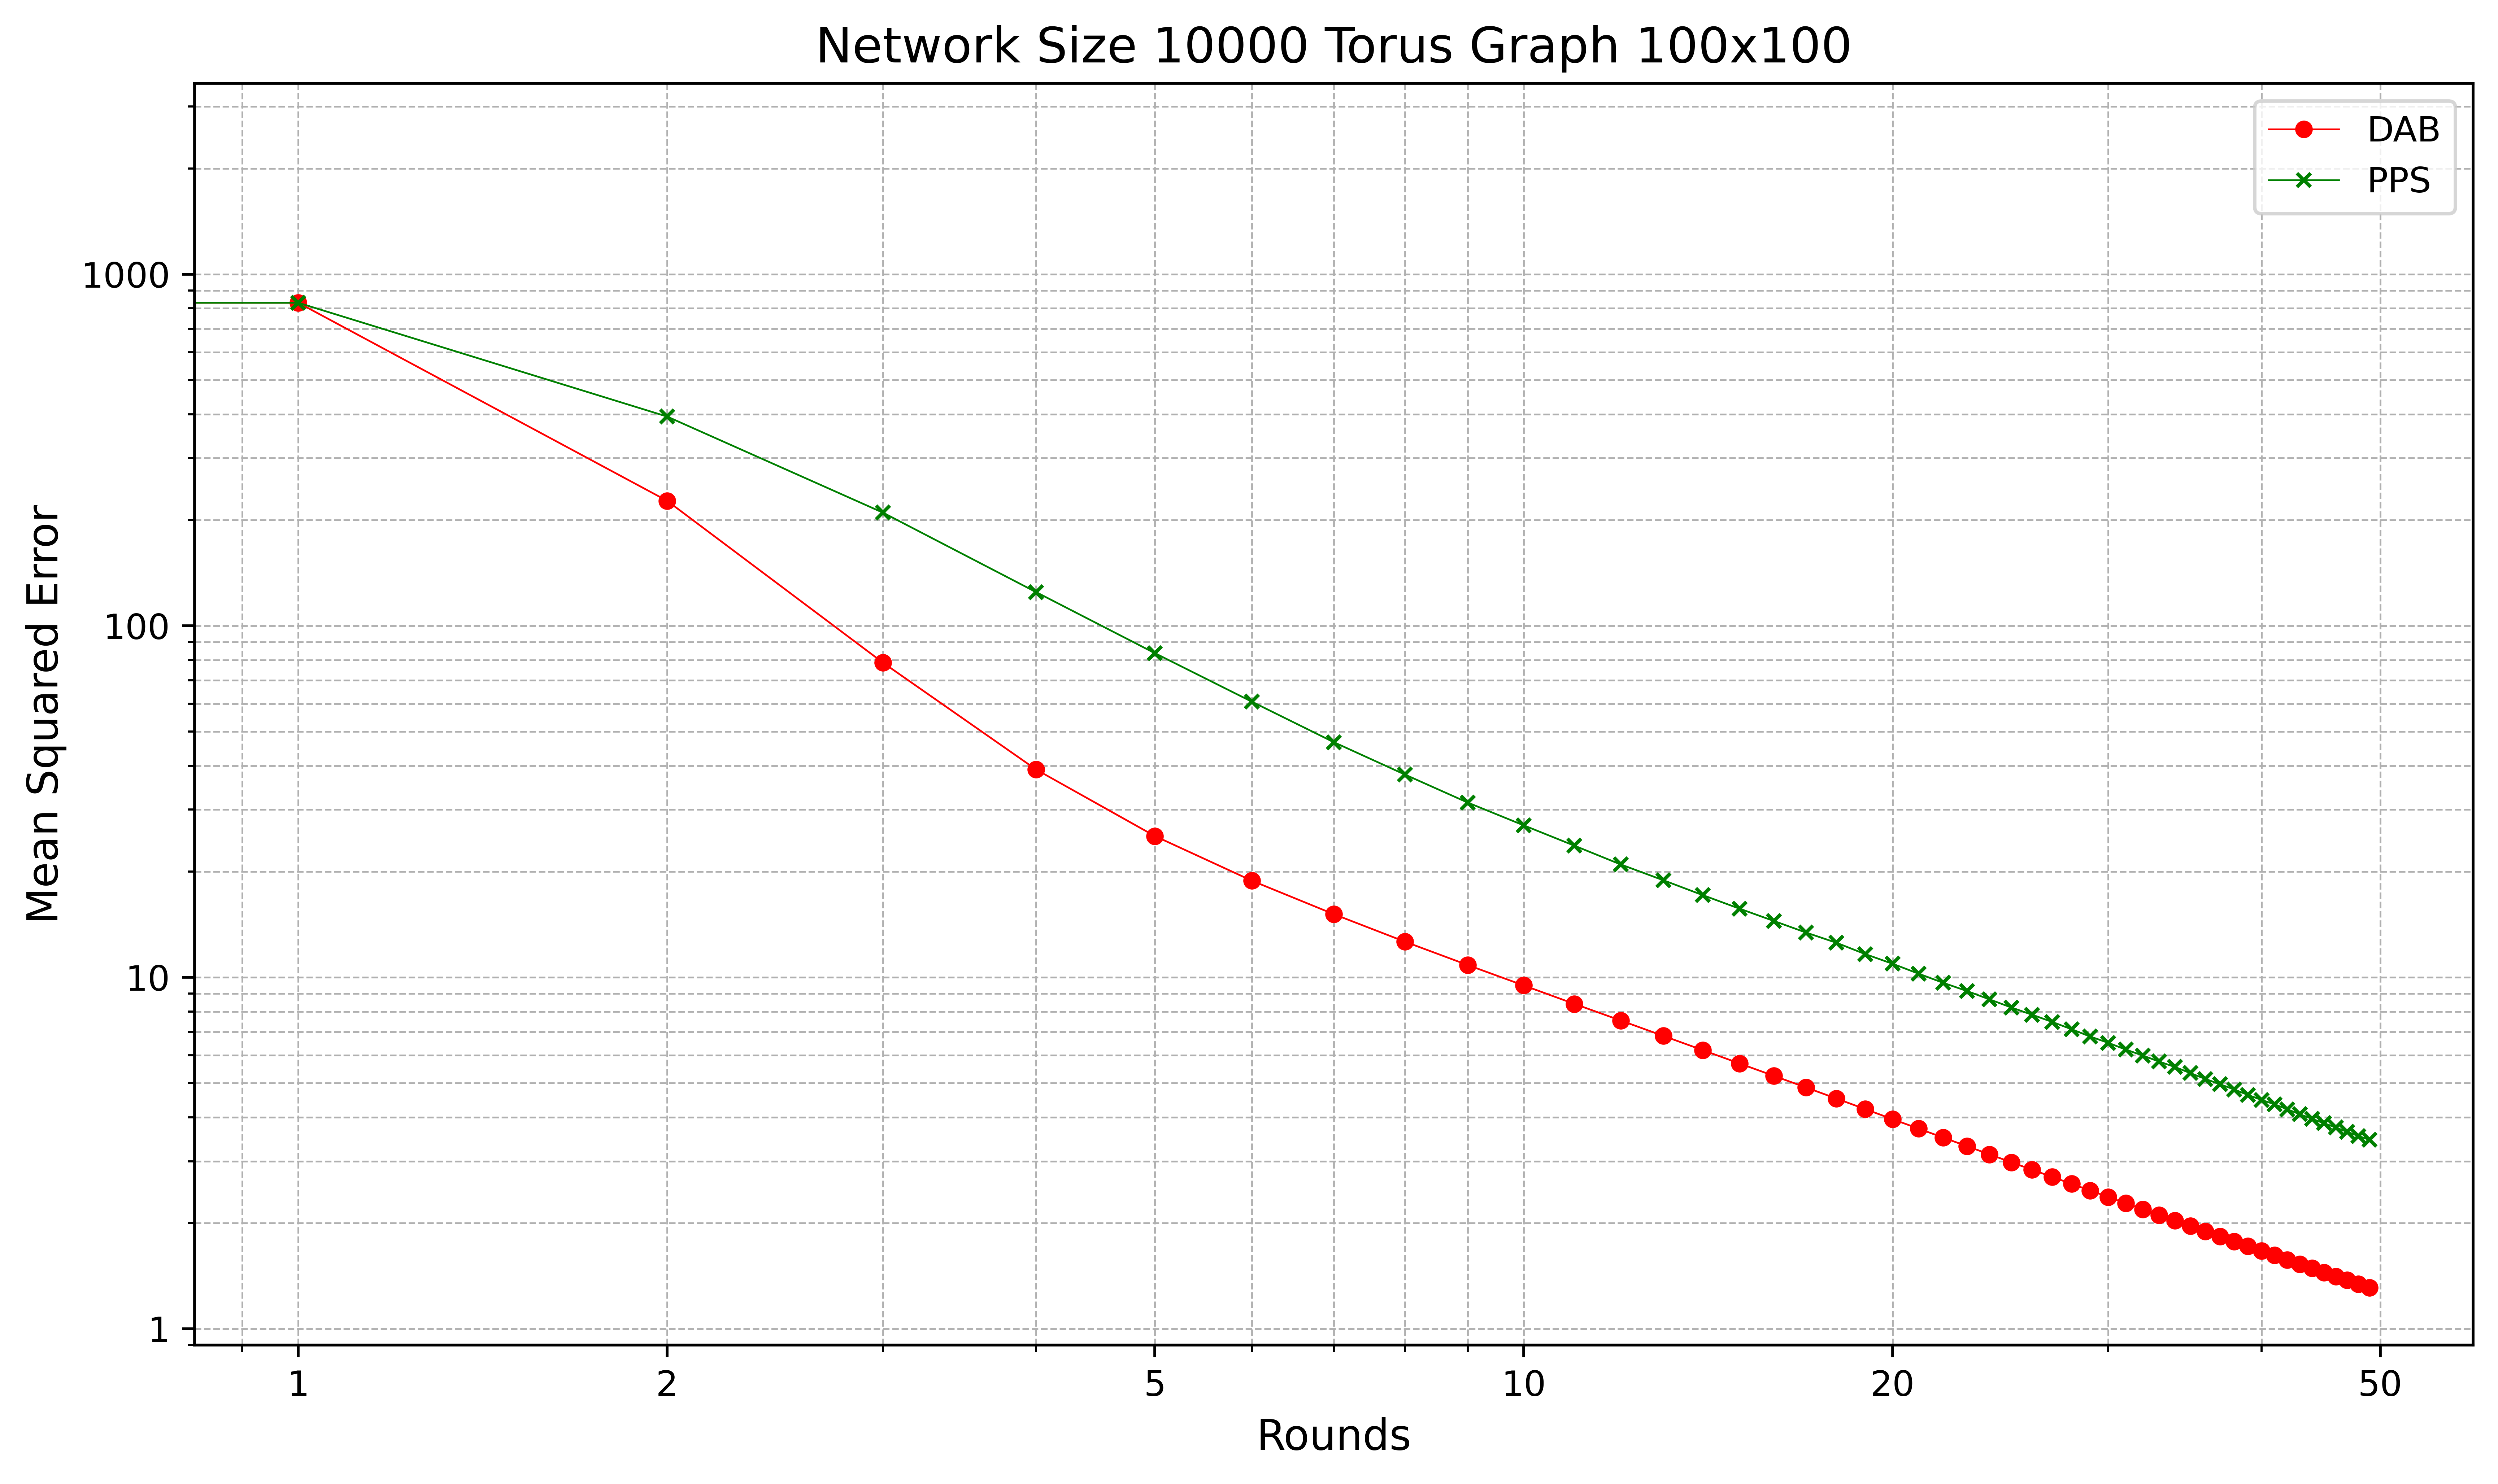
\includegraphics[scale=0.5]{figures/torusGridGraphSimulations/100x100/DAB_vs_PPS_TG_r50_n10000.png}
    \caption{Torus grid graph: network size $10^{4}$ nodes $(1000 \times 10)$}
    \label{fig:100x100Torusgraph}
\end{figure}
\begin{figure}[H]
    \centering
    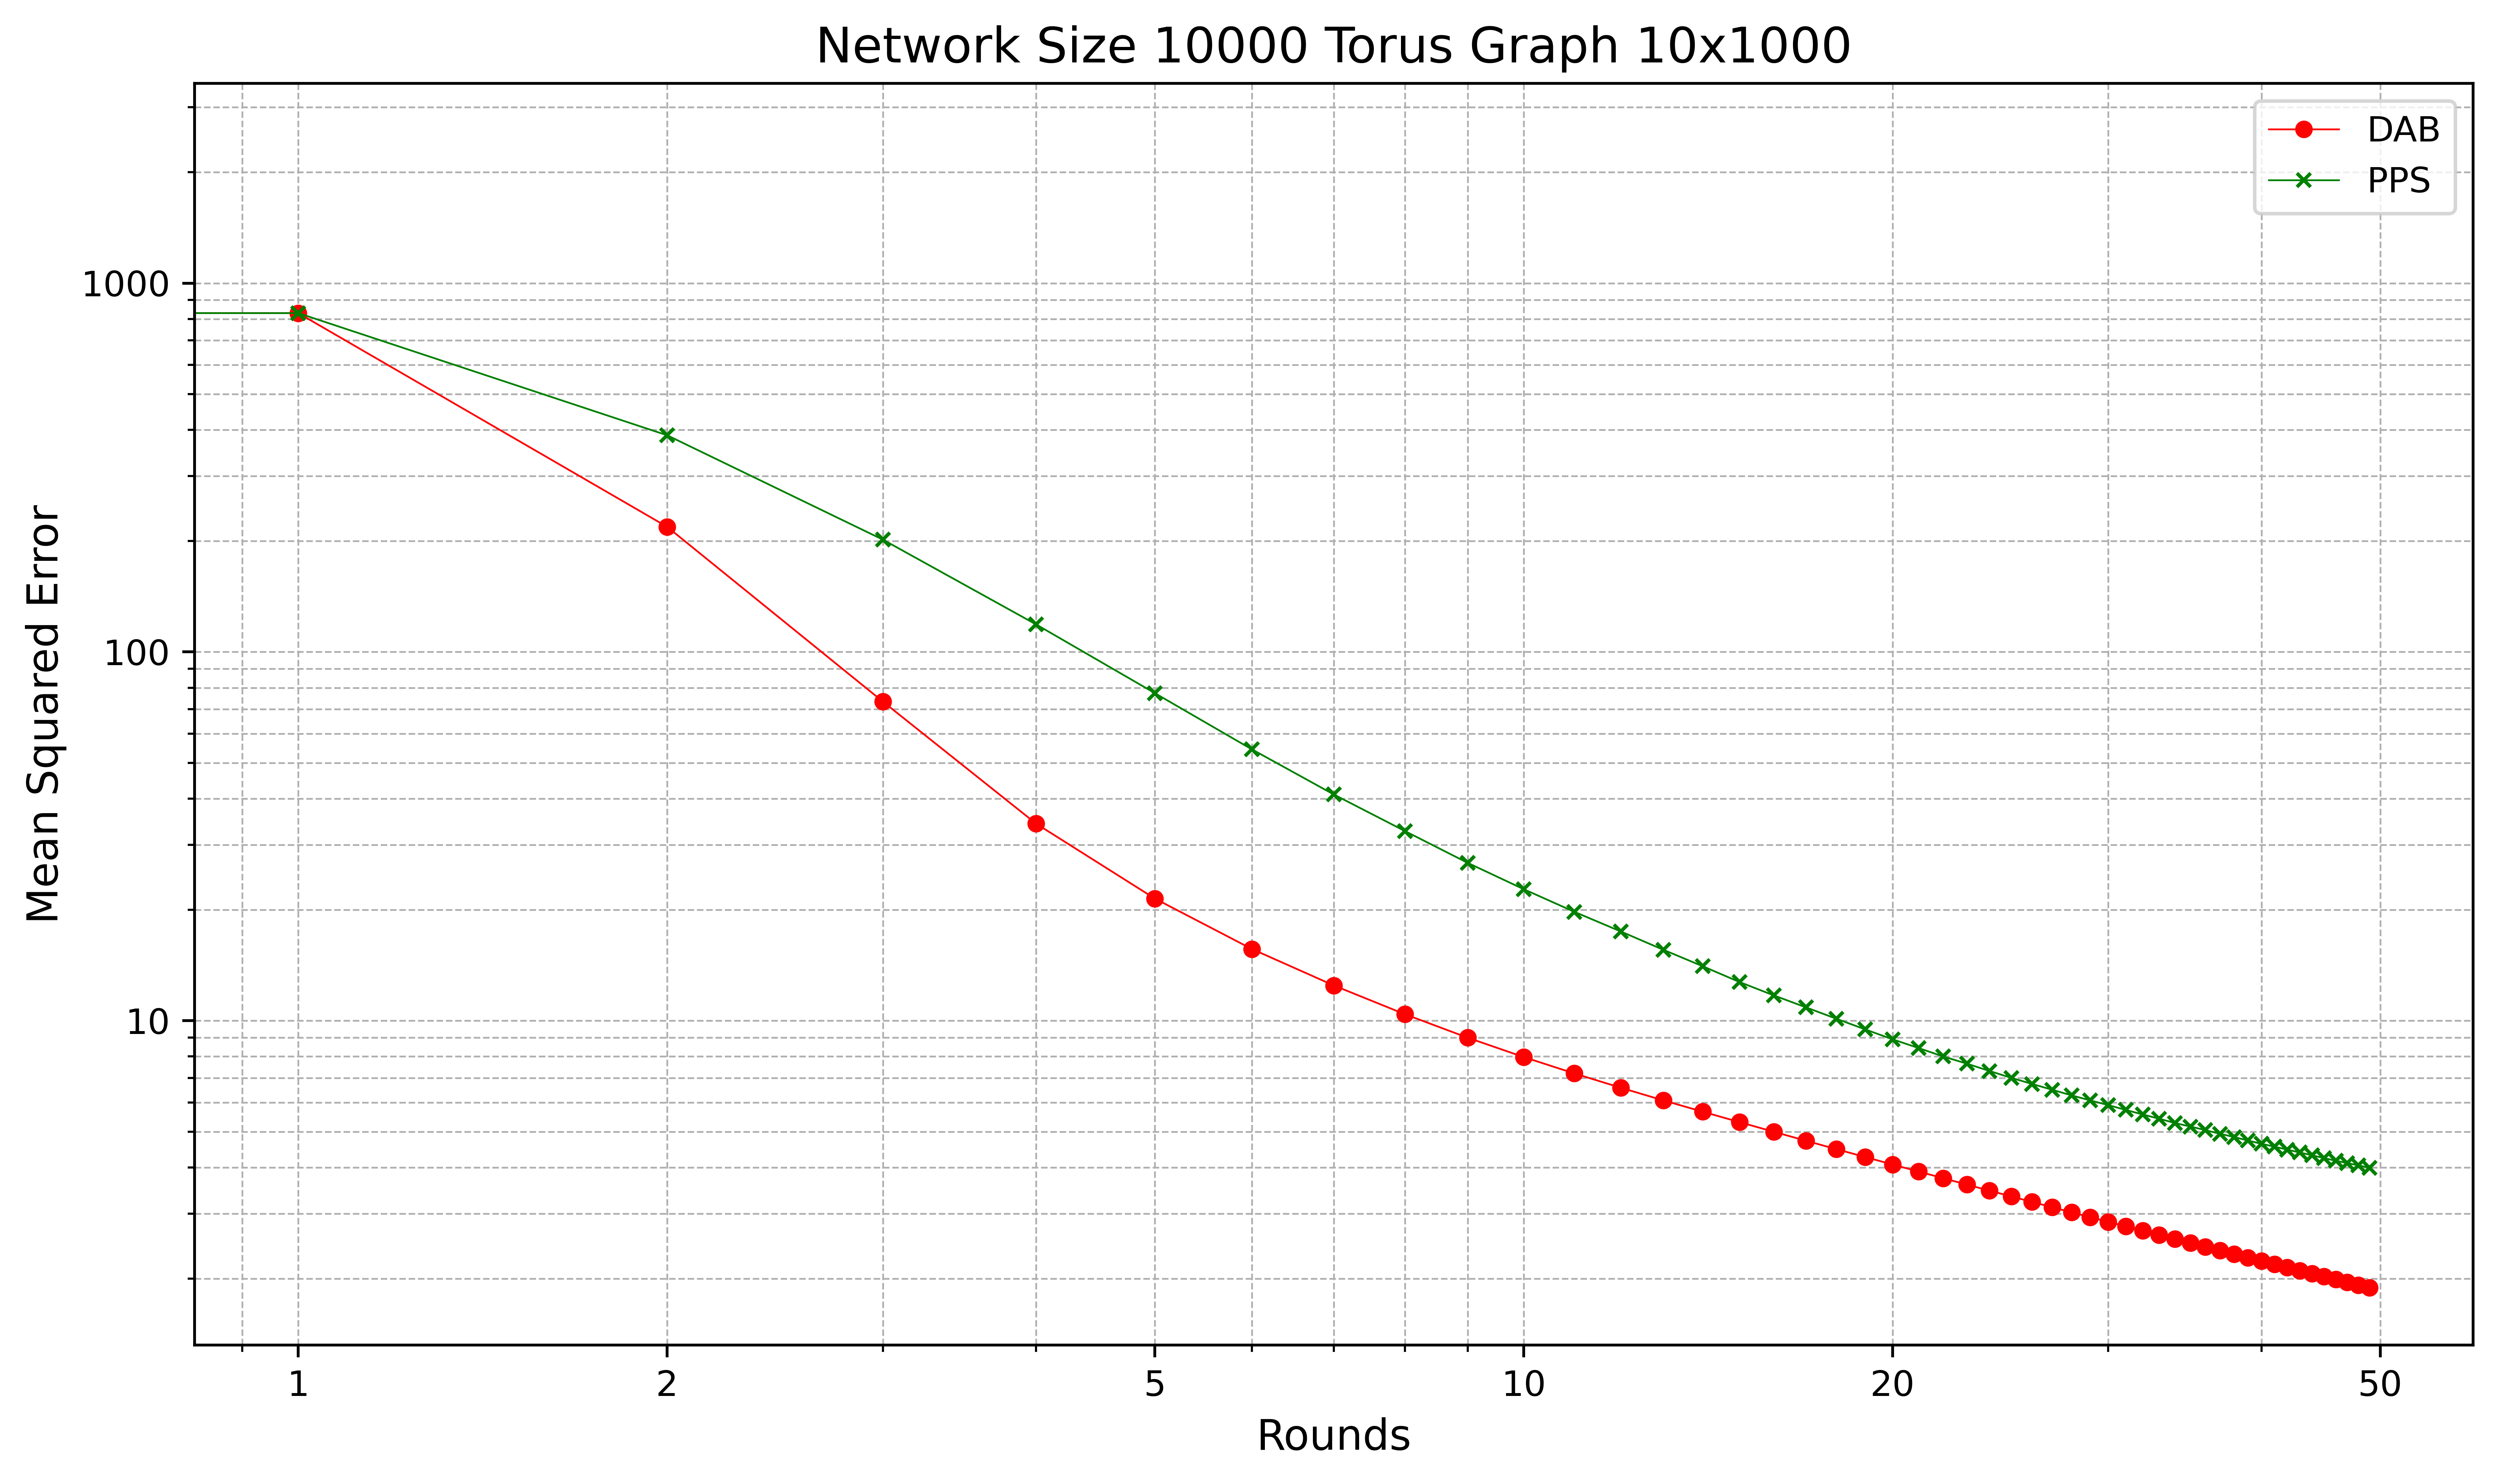
\includegraphics[scale=0.5]{figures/torusGridGraphSimulations/10x1000/DAB_vs_PPS_TG_r50_n10000.png}
    \caption{Torus grid graph: network size $10^{4}$ nodes $(10 \times 1000)$}
    \label{fig:10x1000Torusgraph}
\end{figure}
\begin{figure}[H]
    \centering
    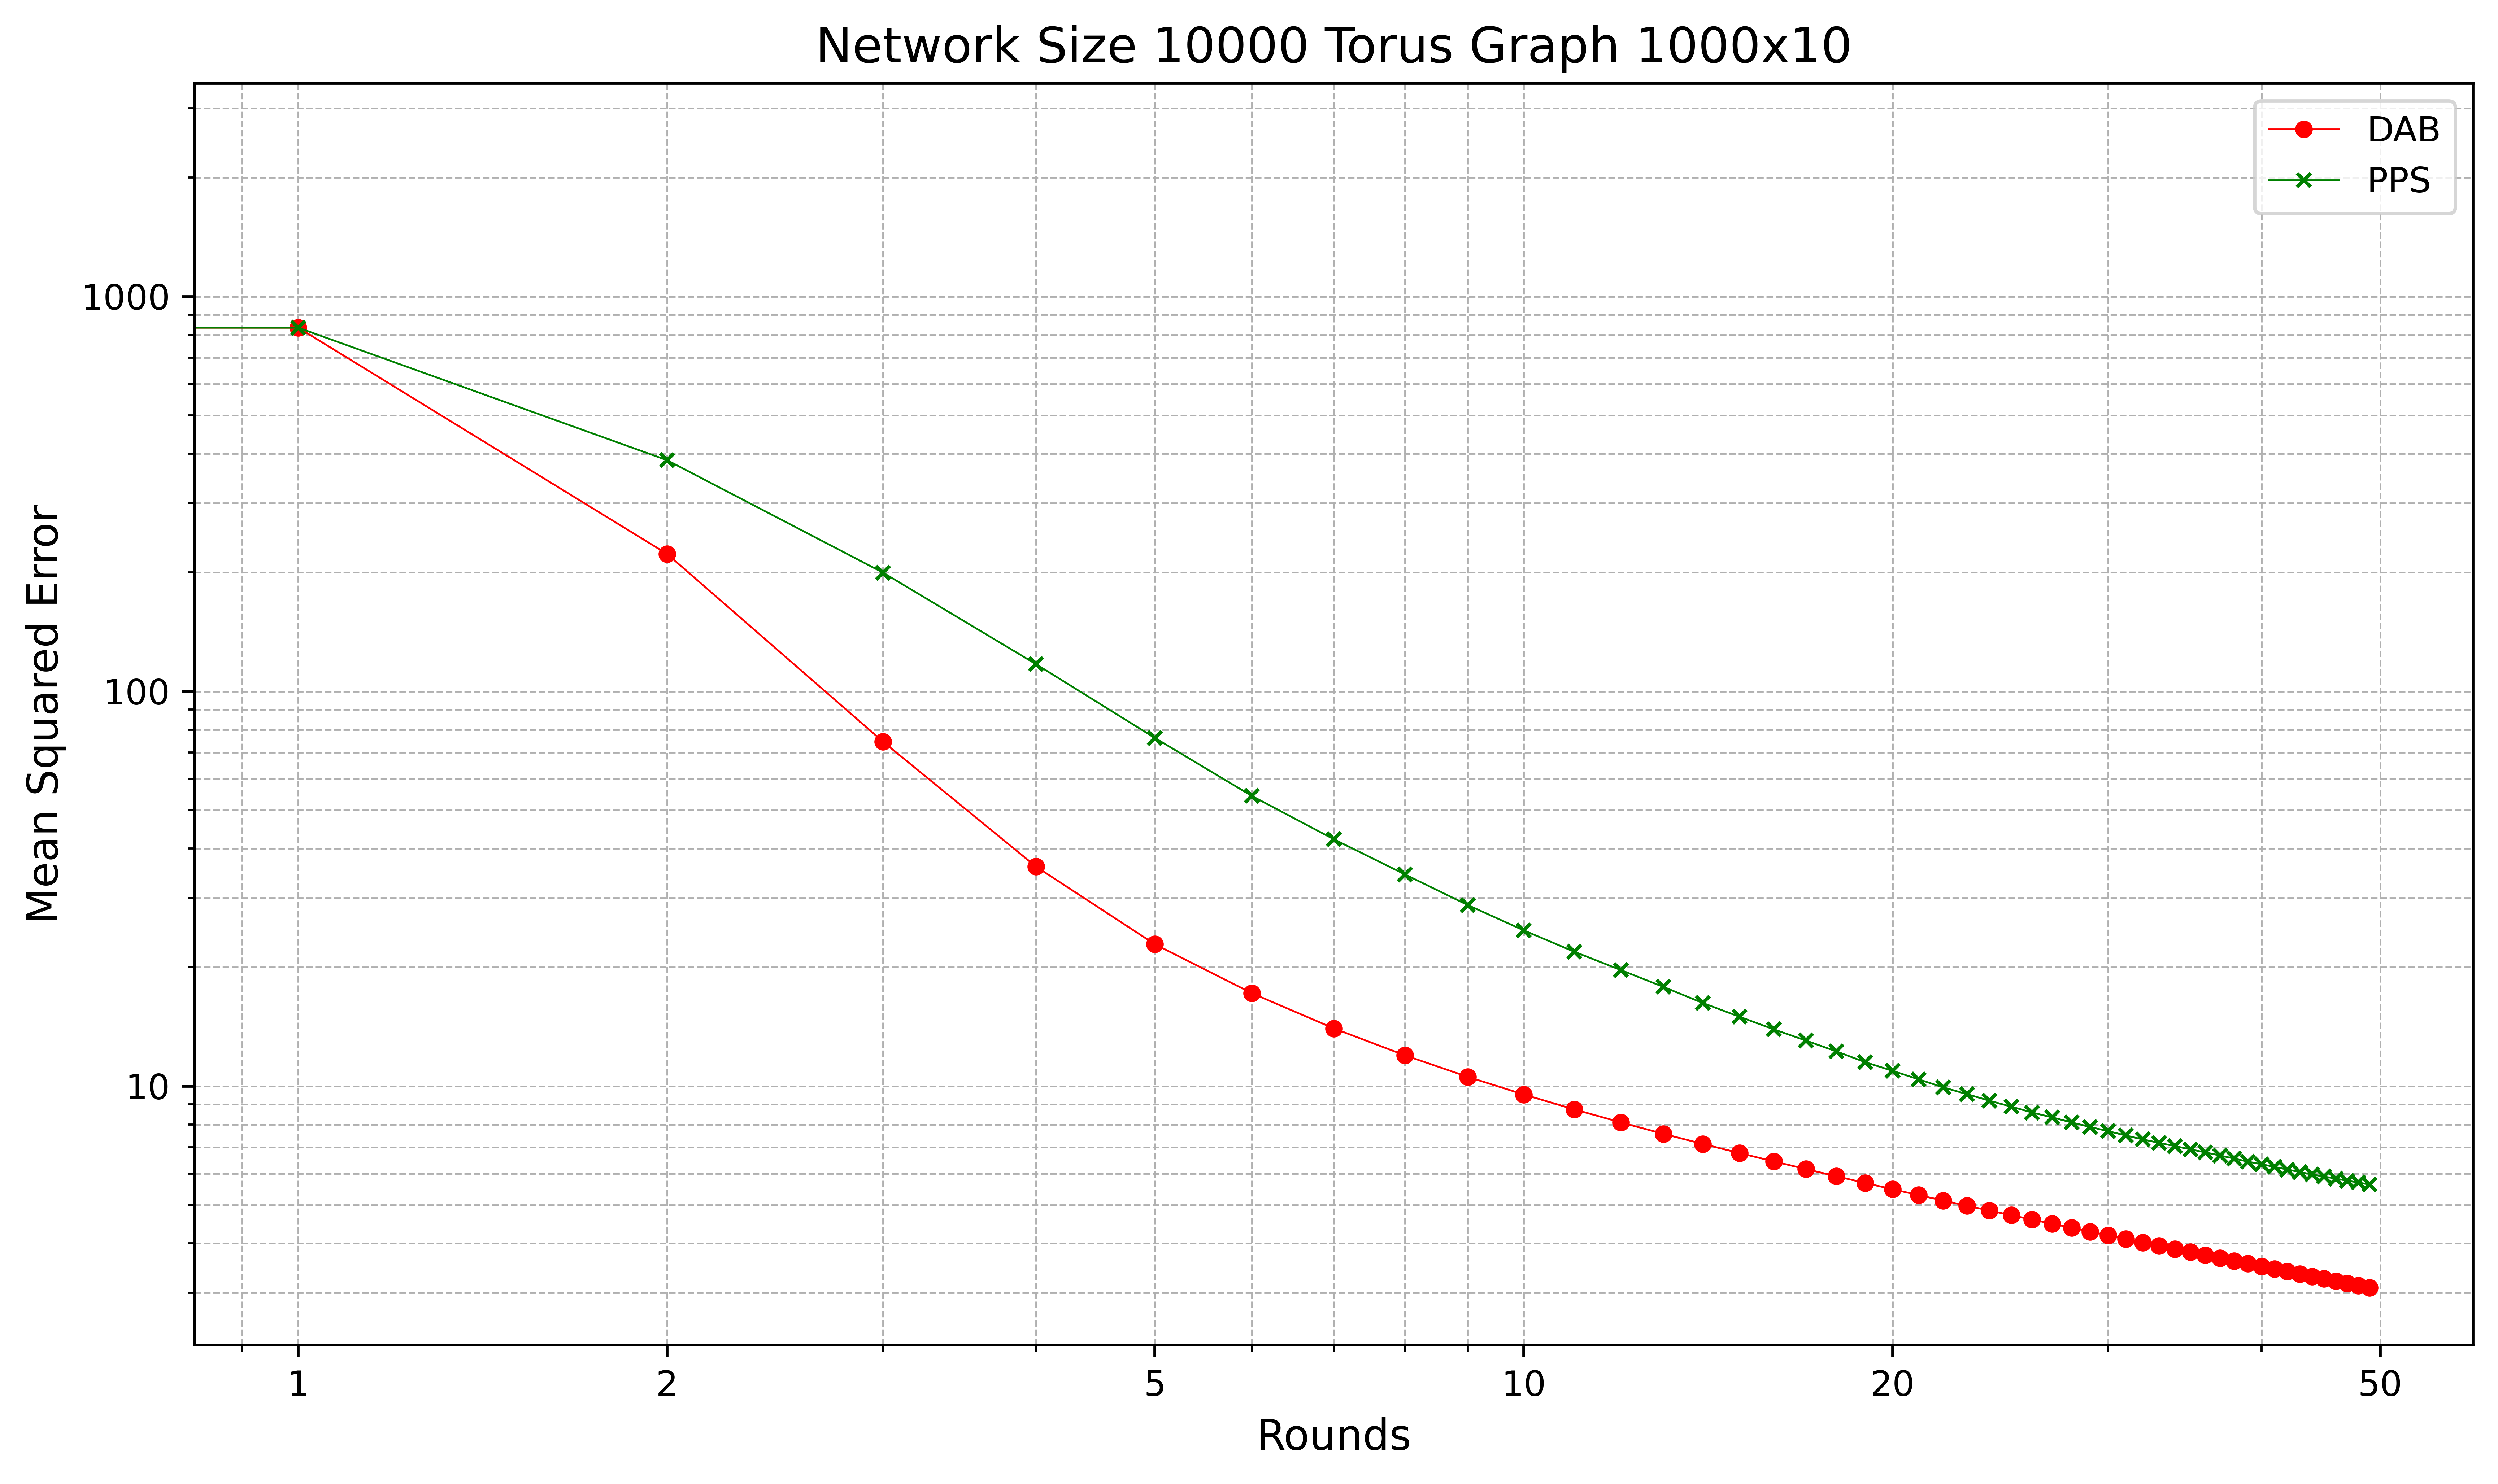
\includegraphics[scale=0.5]{figures/torusGridGraphSimulations/1000x10/DAB_vs_PPS_TG_r50_n10000.png}
    \caption{Torus grid graph: network size $10^{4}$ nodes $(1000 \times 10)$}
    \label{fig:1000x10Torusgraph}
\end{figure}

\subsection{Ring of Cliques}
\begin{figure}[H]
    \centering
    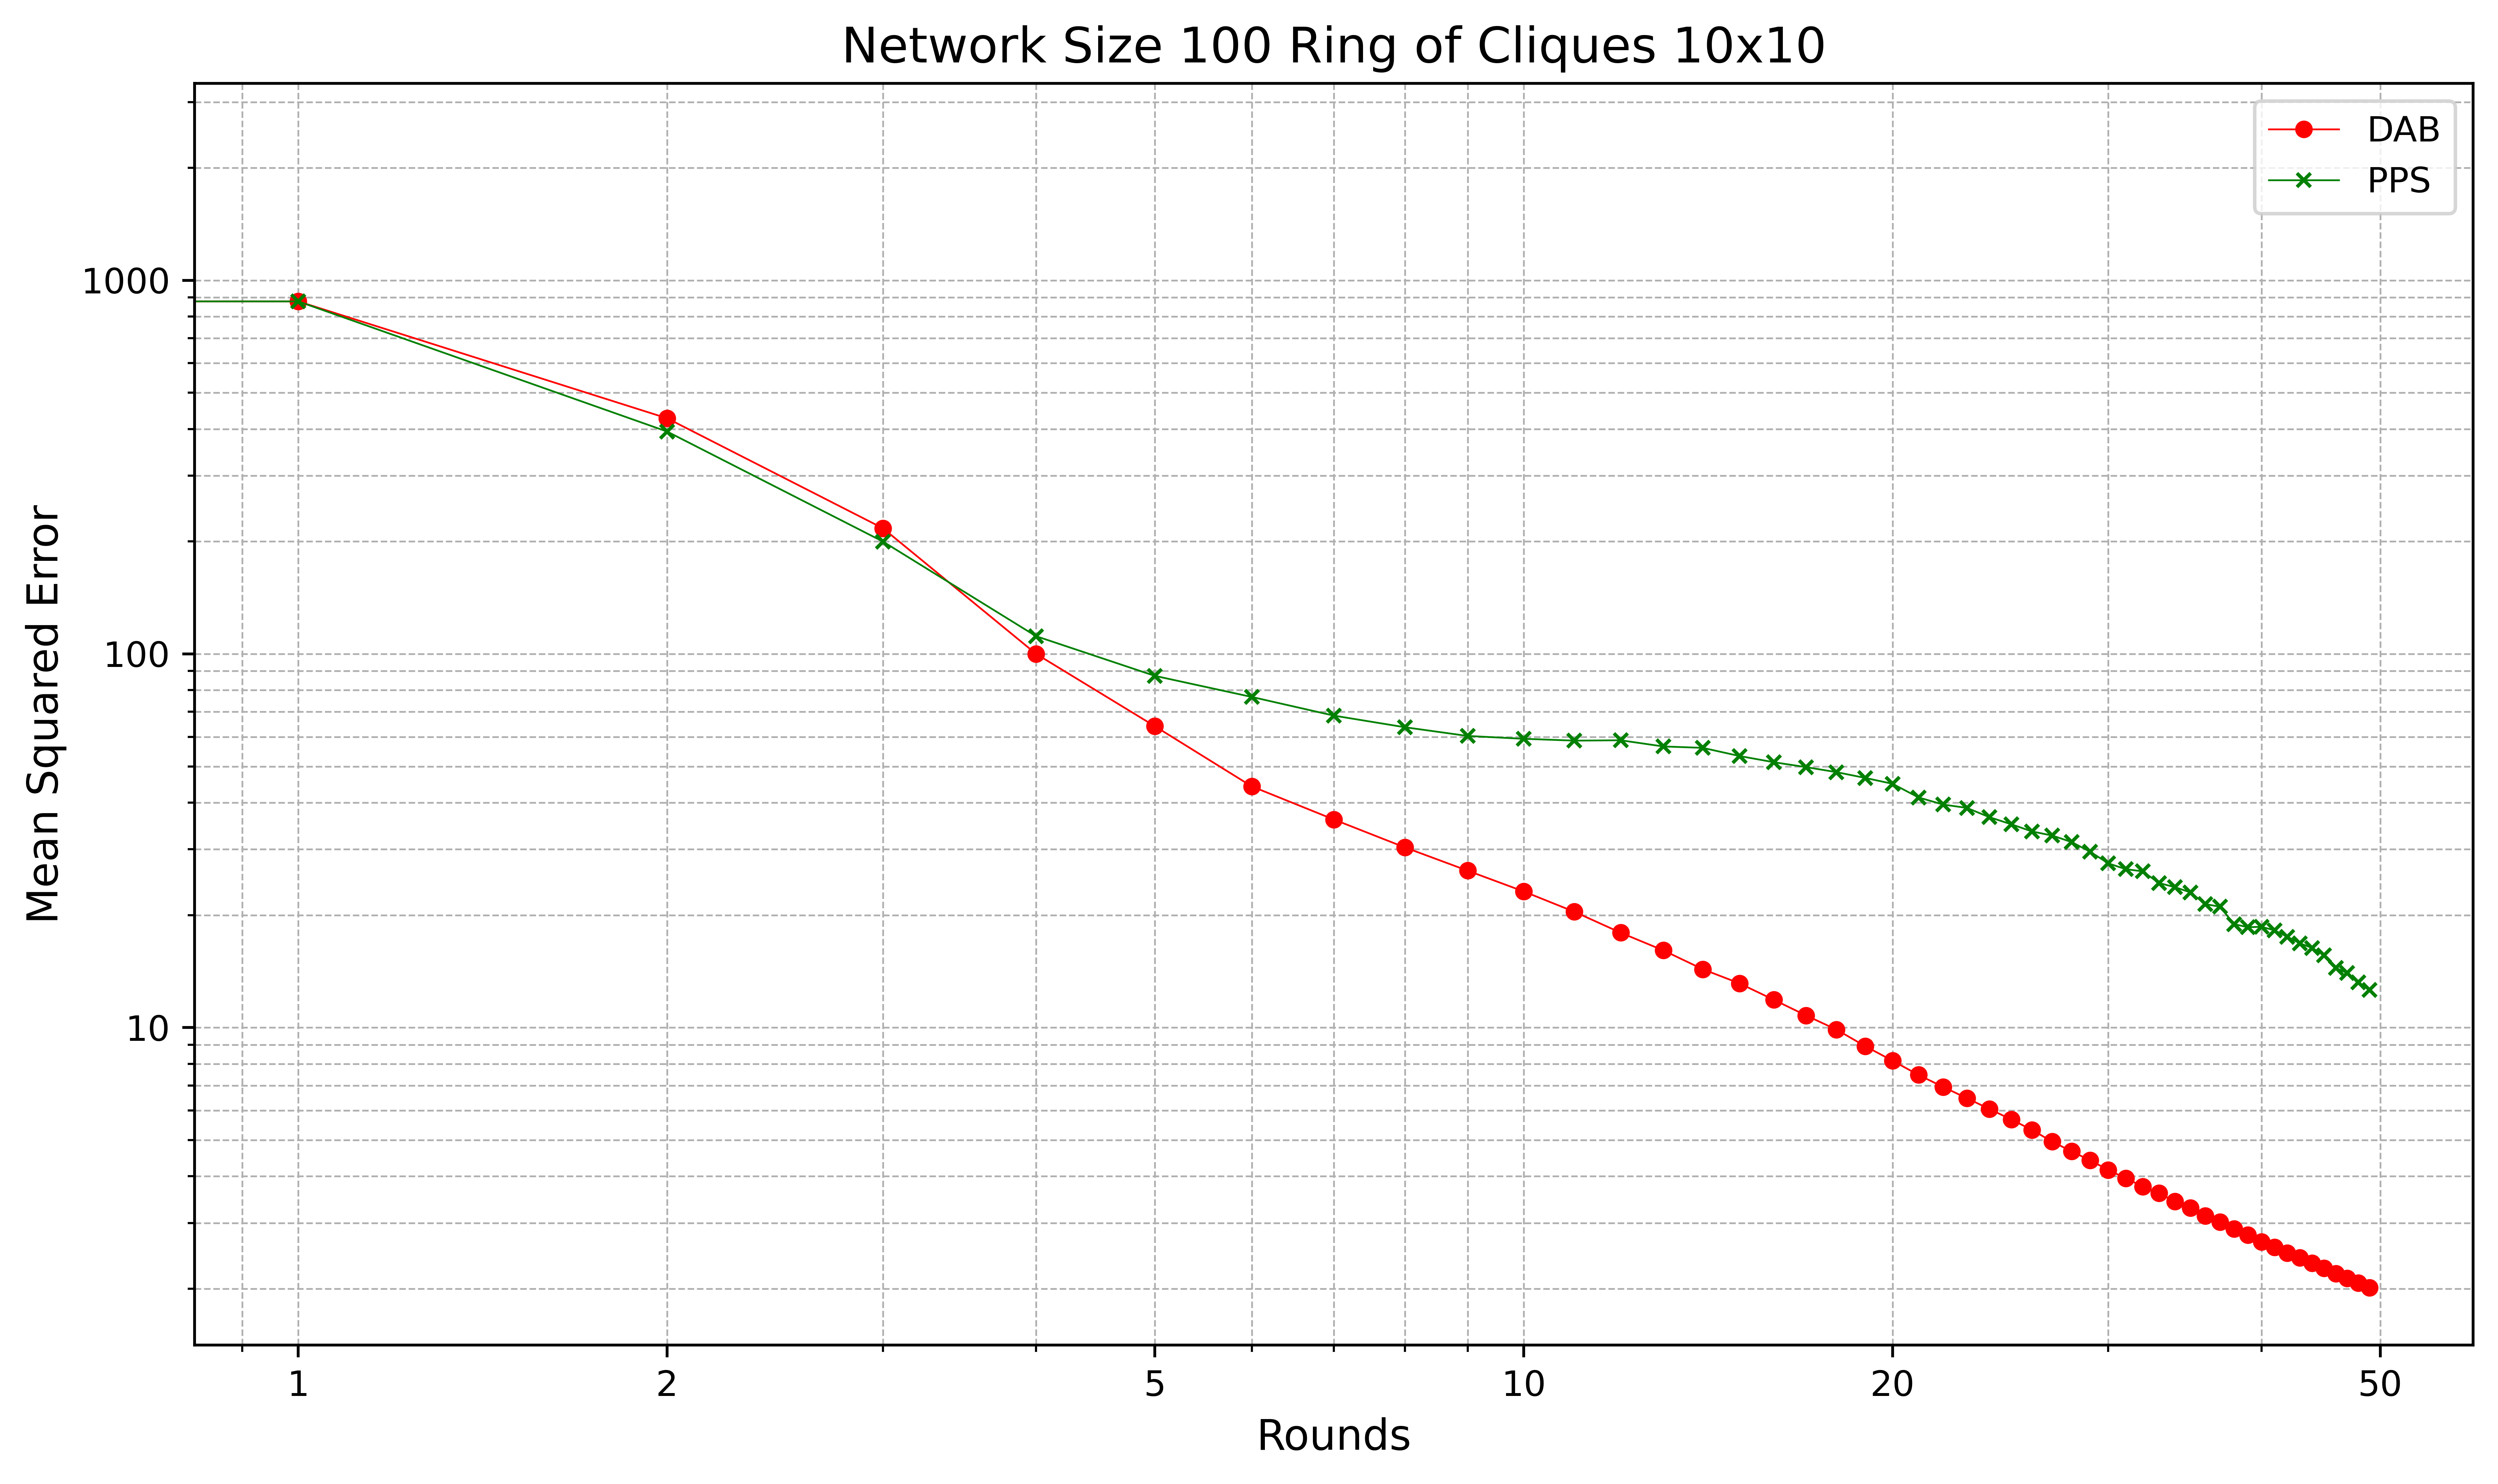
\includegraphics[scale=0.5]{figures/ringOfCliquesSimulations/DAB_vs_PPS_RoC_r50_n100.png}
    \caption{Ring of cliques: network size $10^{2}$ nodes $(10 \times 10)$}
    \label{fig:10x10RingOfCliques}
\end{figure}
\begin{figure}[H]
    \centering
    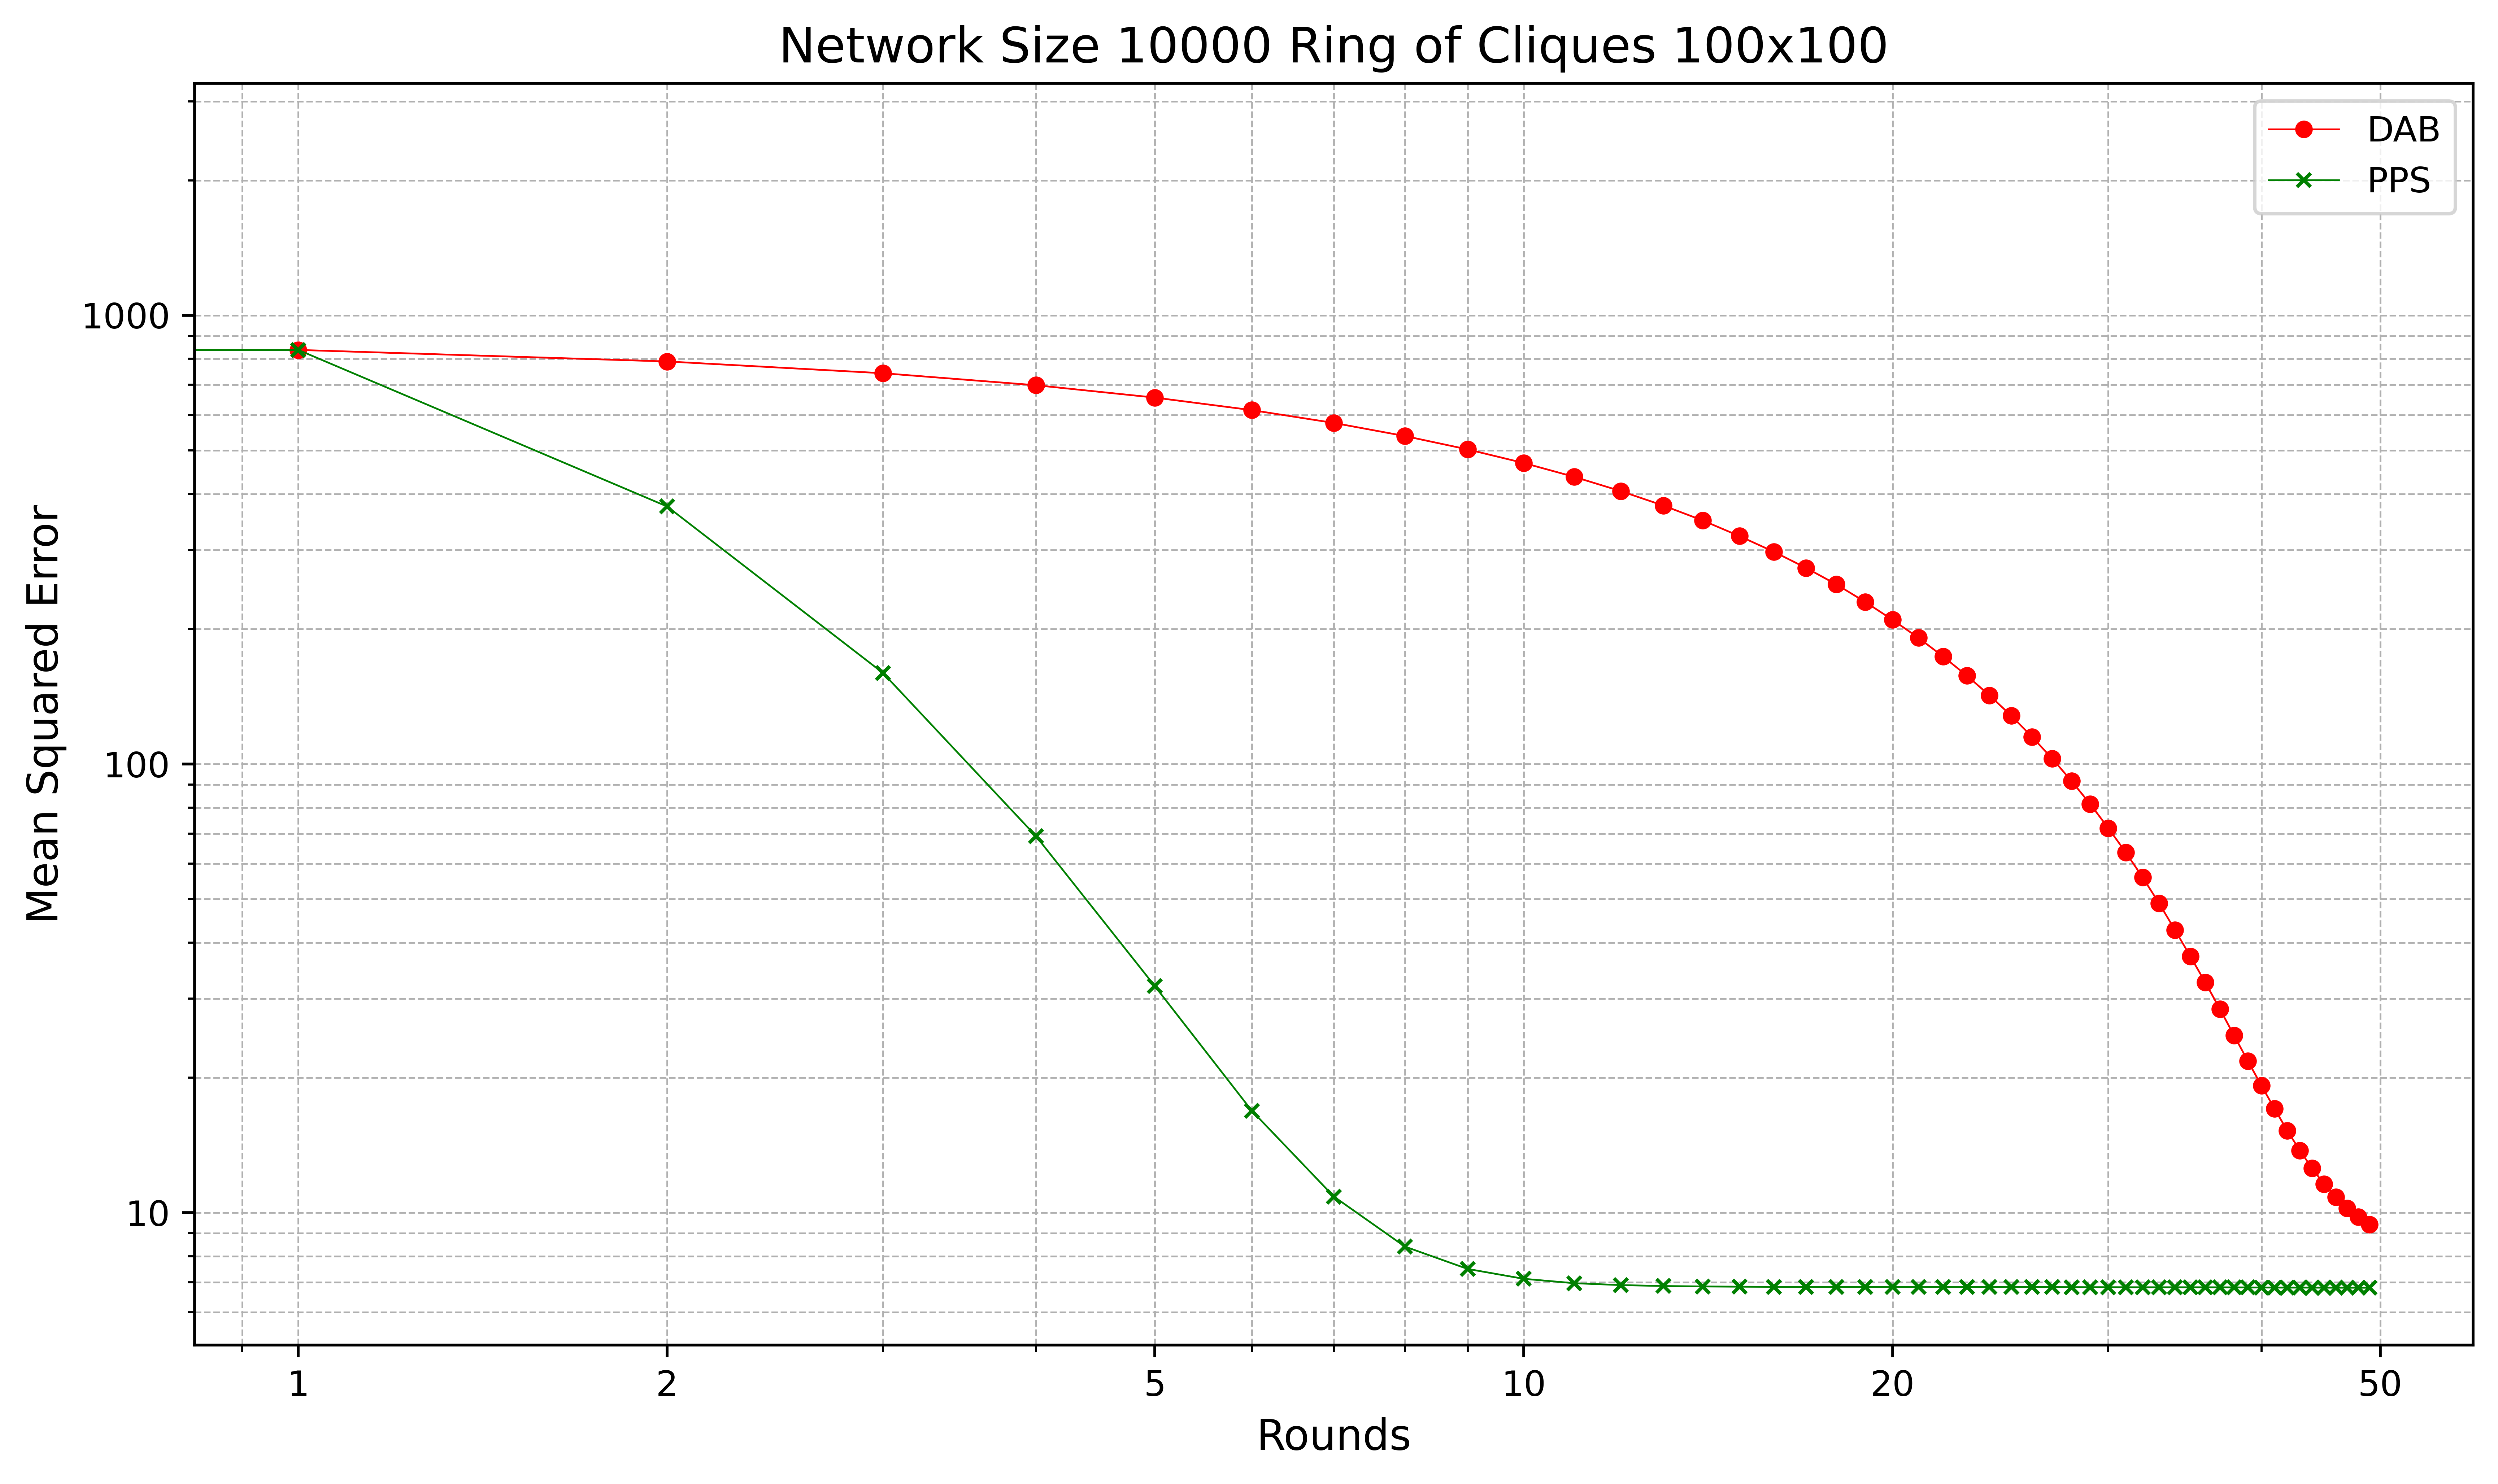
\includegraphics[scale=0.5]{figures/ringOfCliquesSimulations/100x100/DAB_vs_PPS_RoC_r50_n10000.png}
    \caption{Ring of cliques: network size $10^{4}$ nodes $(100 \times 100)$}
    \label{fig:100x100RingOfCliques}
\end{figure}
\begin{figure}[H]
    \centering
    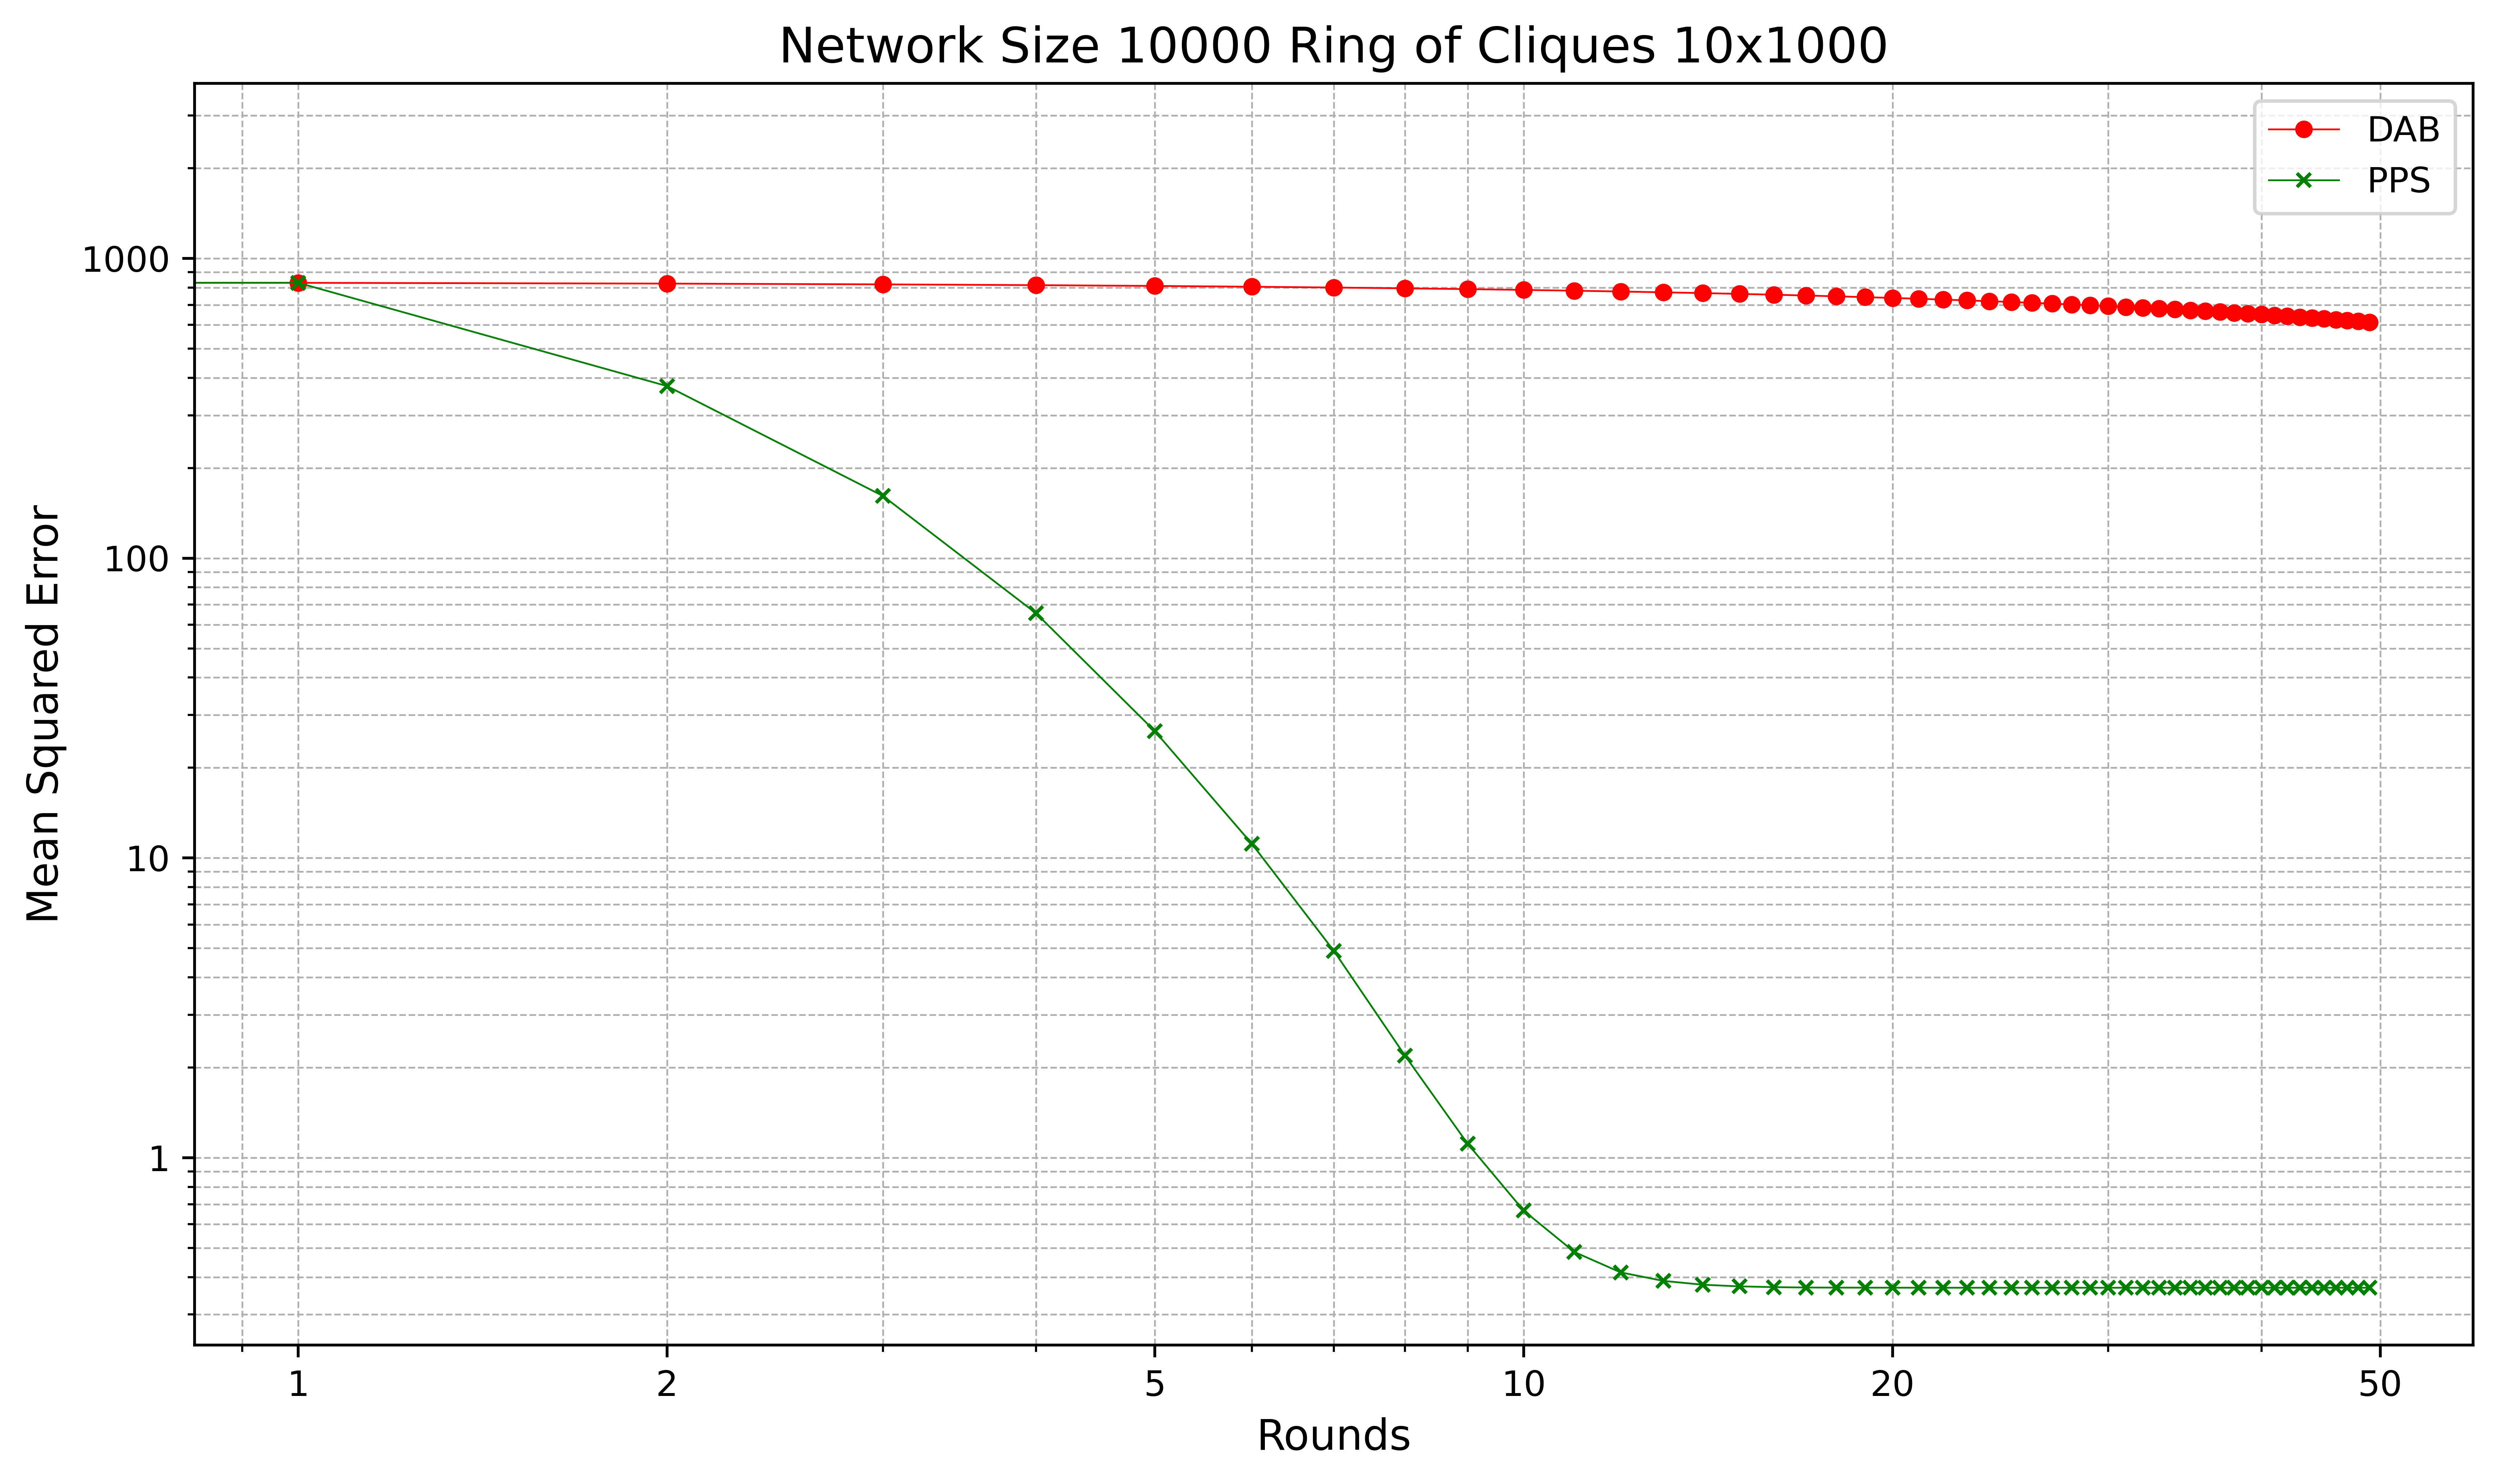
\includegraphics[scale=0.5]{figures/ringOfCliquesSimulations/10x1000/DAB_vs_PPS_RoC_r50_n10000.png}
    \caption{Ring of cliques: network size $10^{4}$ nodes $(10 \times 1000)$}
    \label{fig:10x1000RingOfCliques}
\end{figure}\begin{figure}[H]
    \centering
    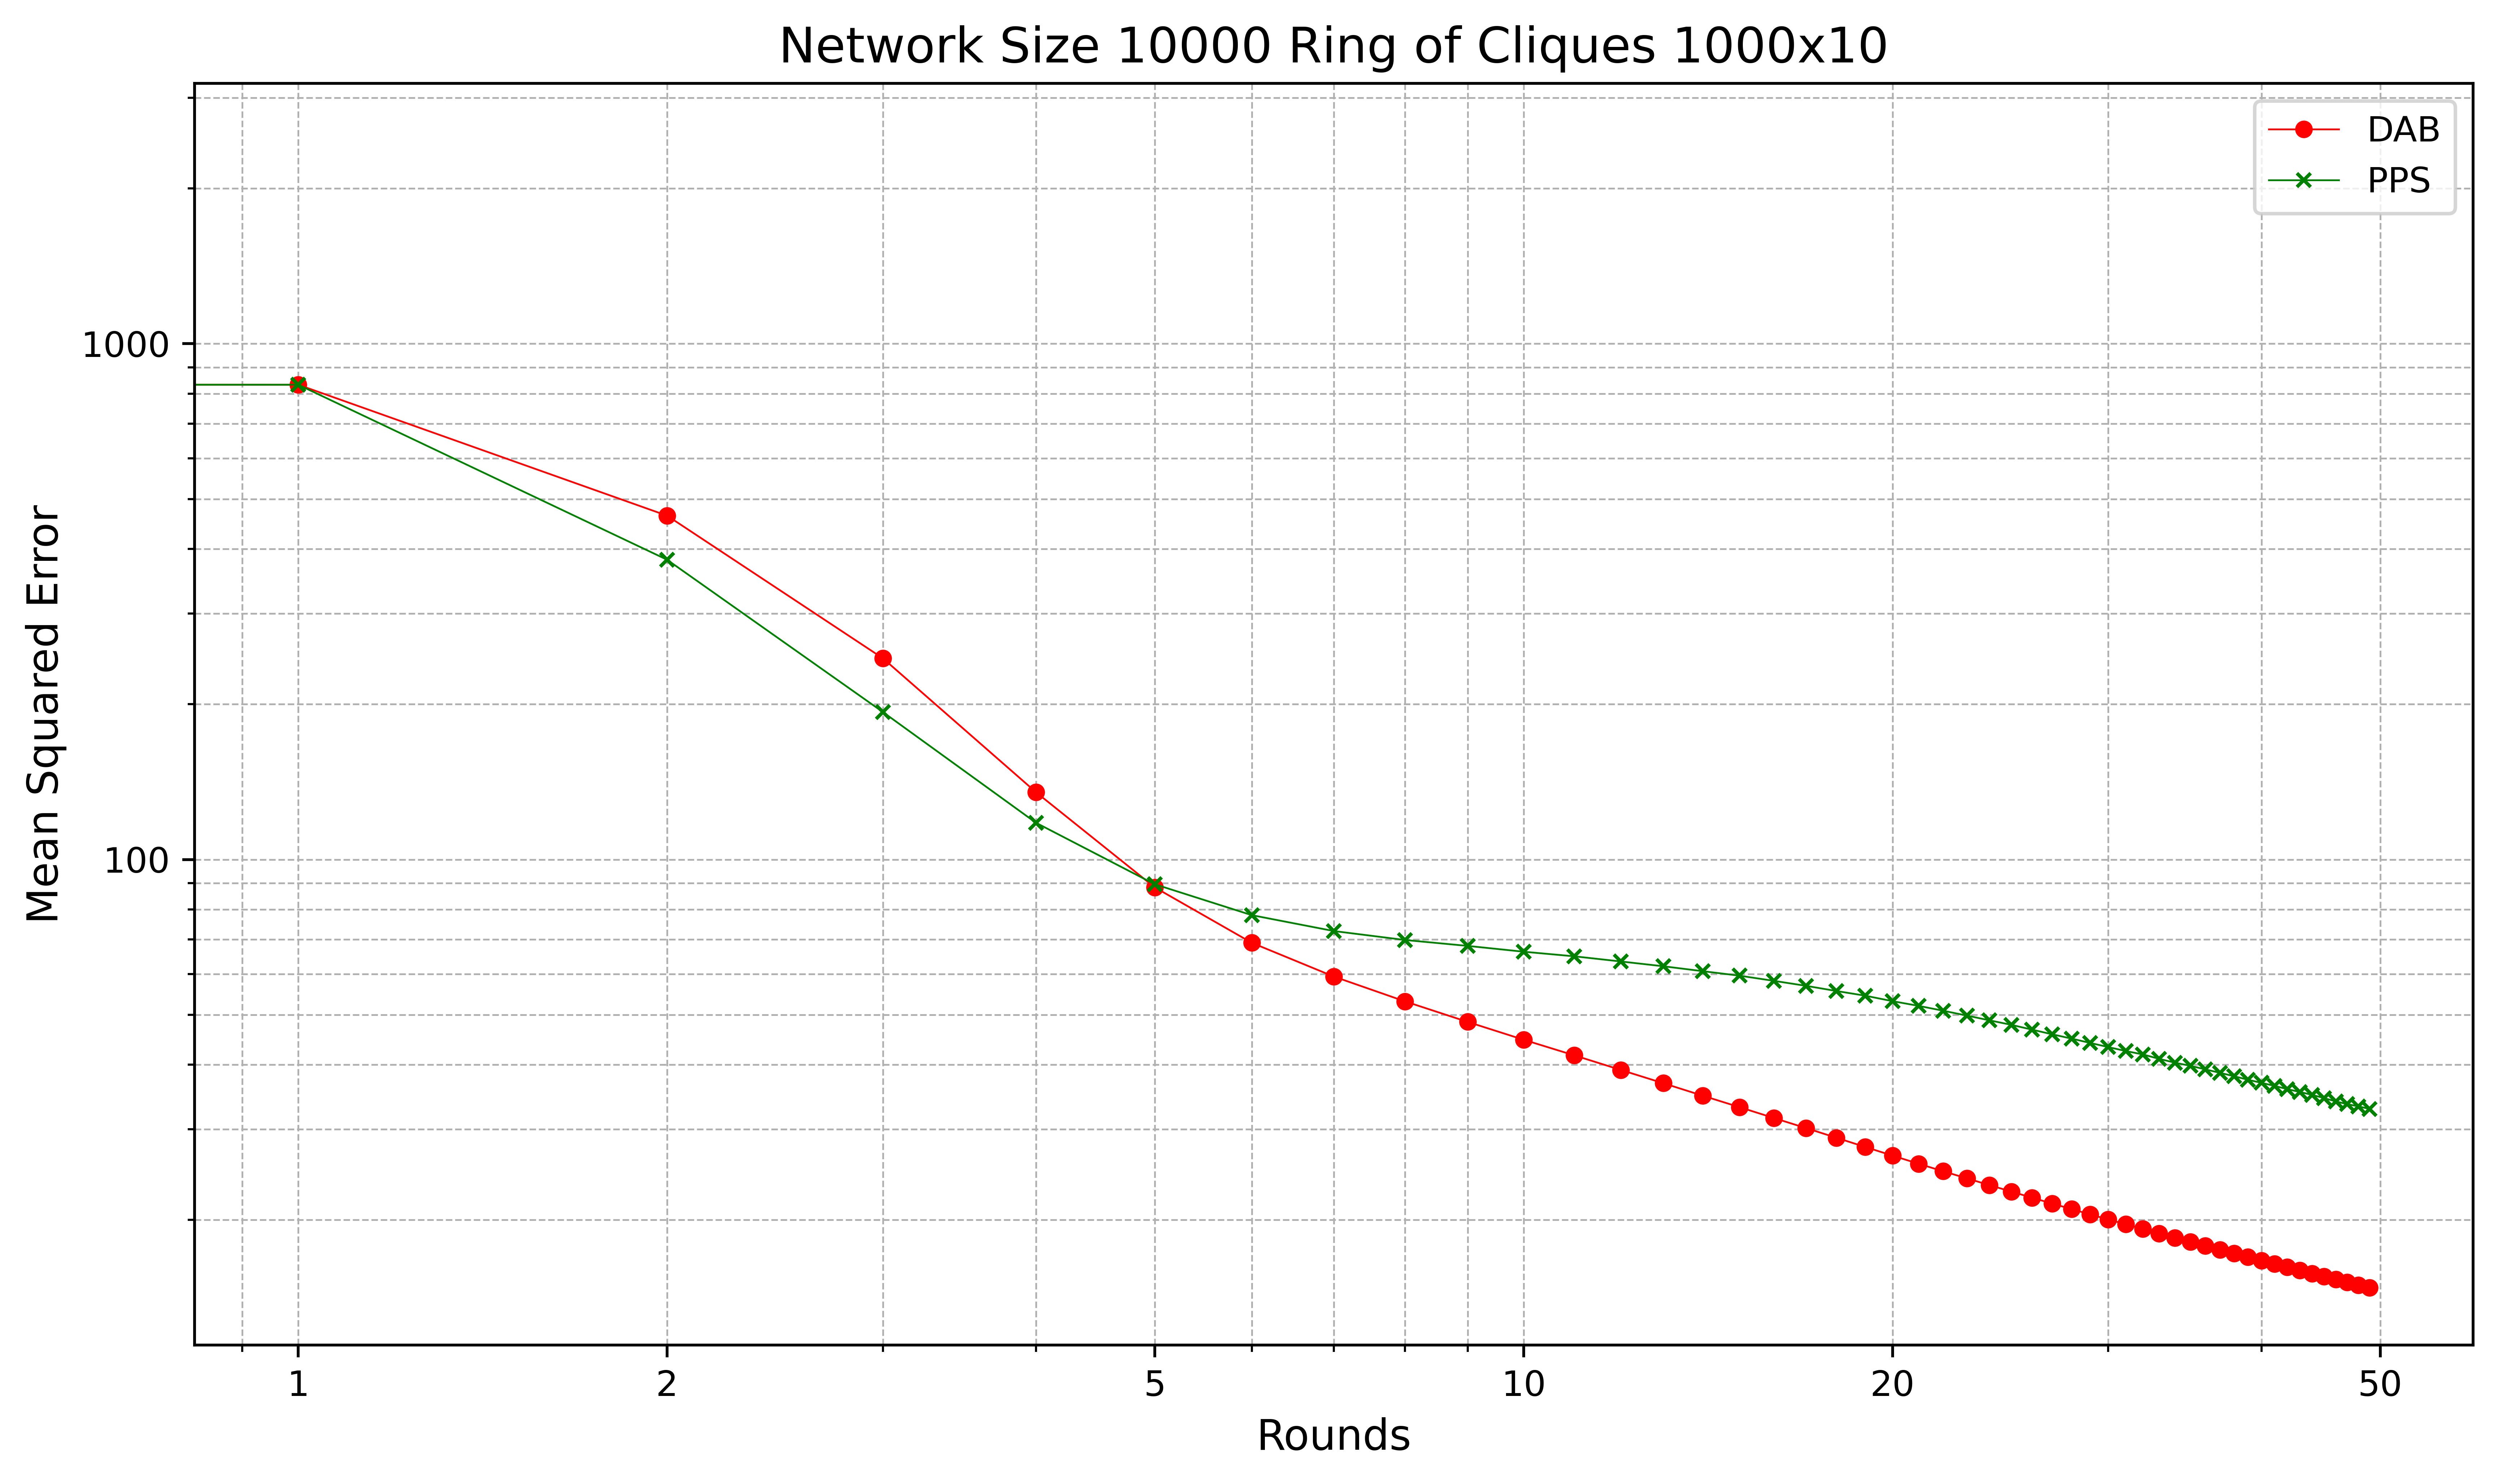
\includegraphics[scale=0.5]{figures/ringOfCliquesSimulations/1000x10/DAB_vs_PPS_RoC_r50_n10000.png}
    \caption{Ring of cliques: network size $10^{4}$ nodes $(1000 \times 10)$}
    \label{fig:1000x10RingOfCliques}
\end{figure}

\subsection{Lollipop Graph}
\begin{figure}[H]
    \centering
    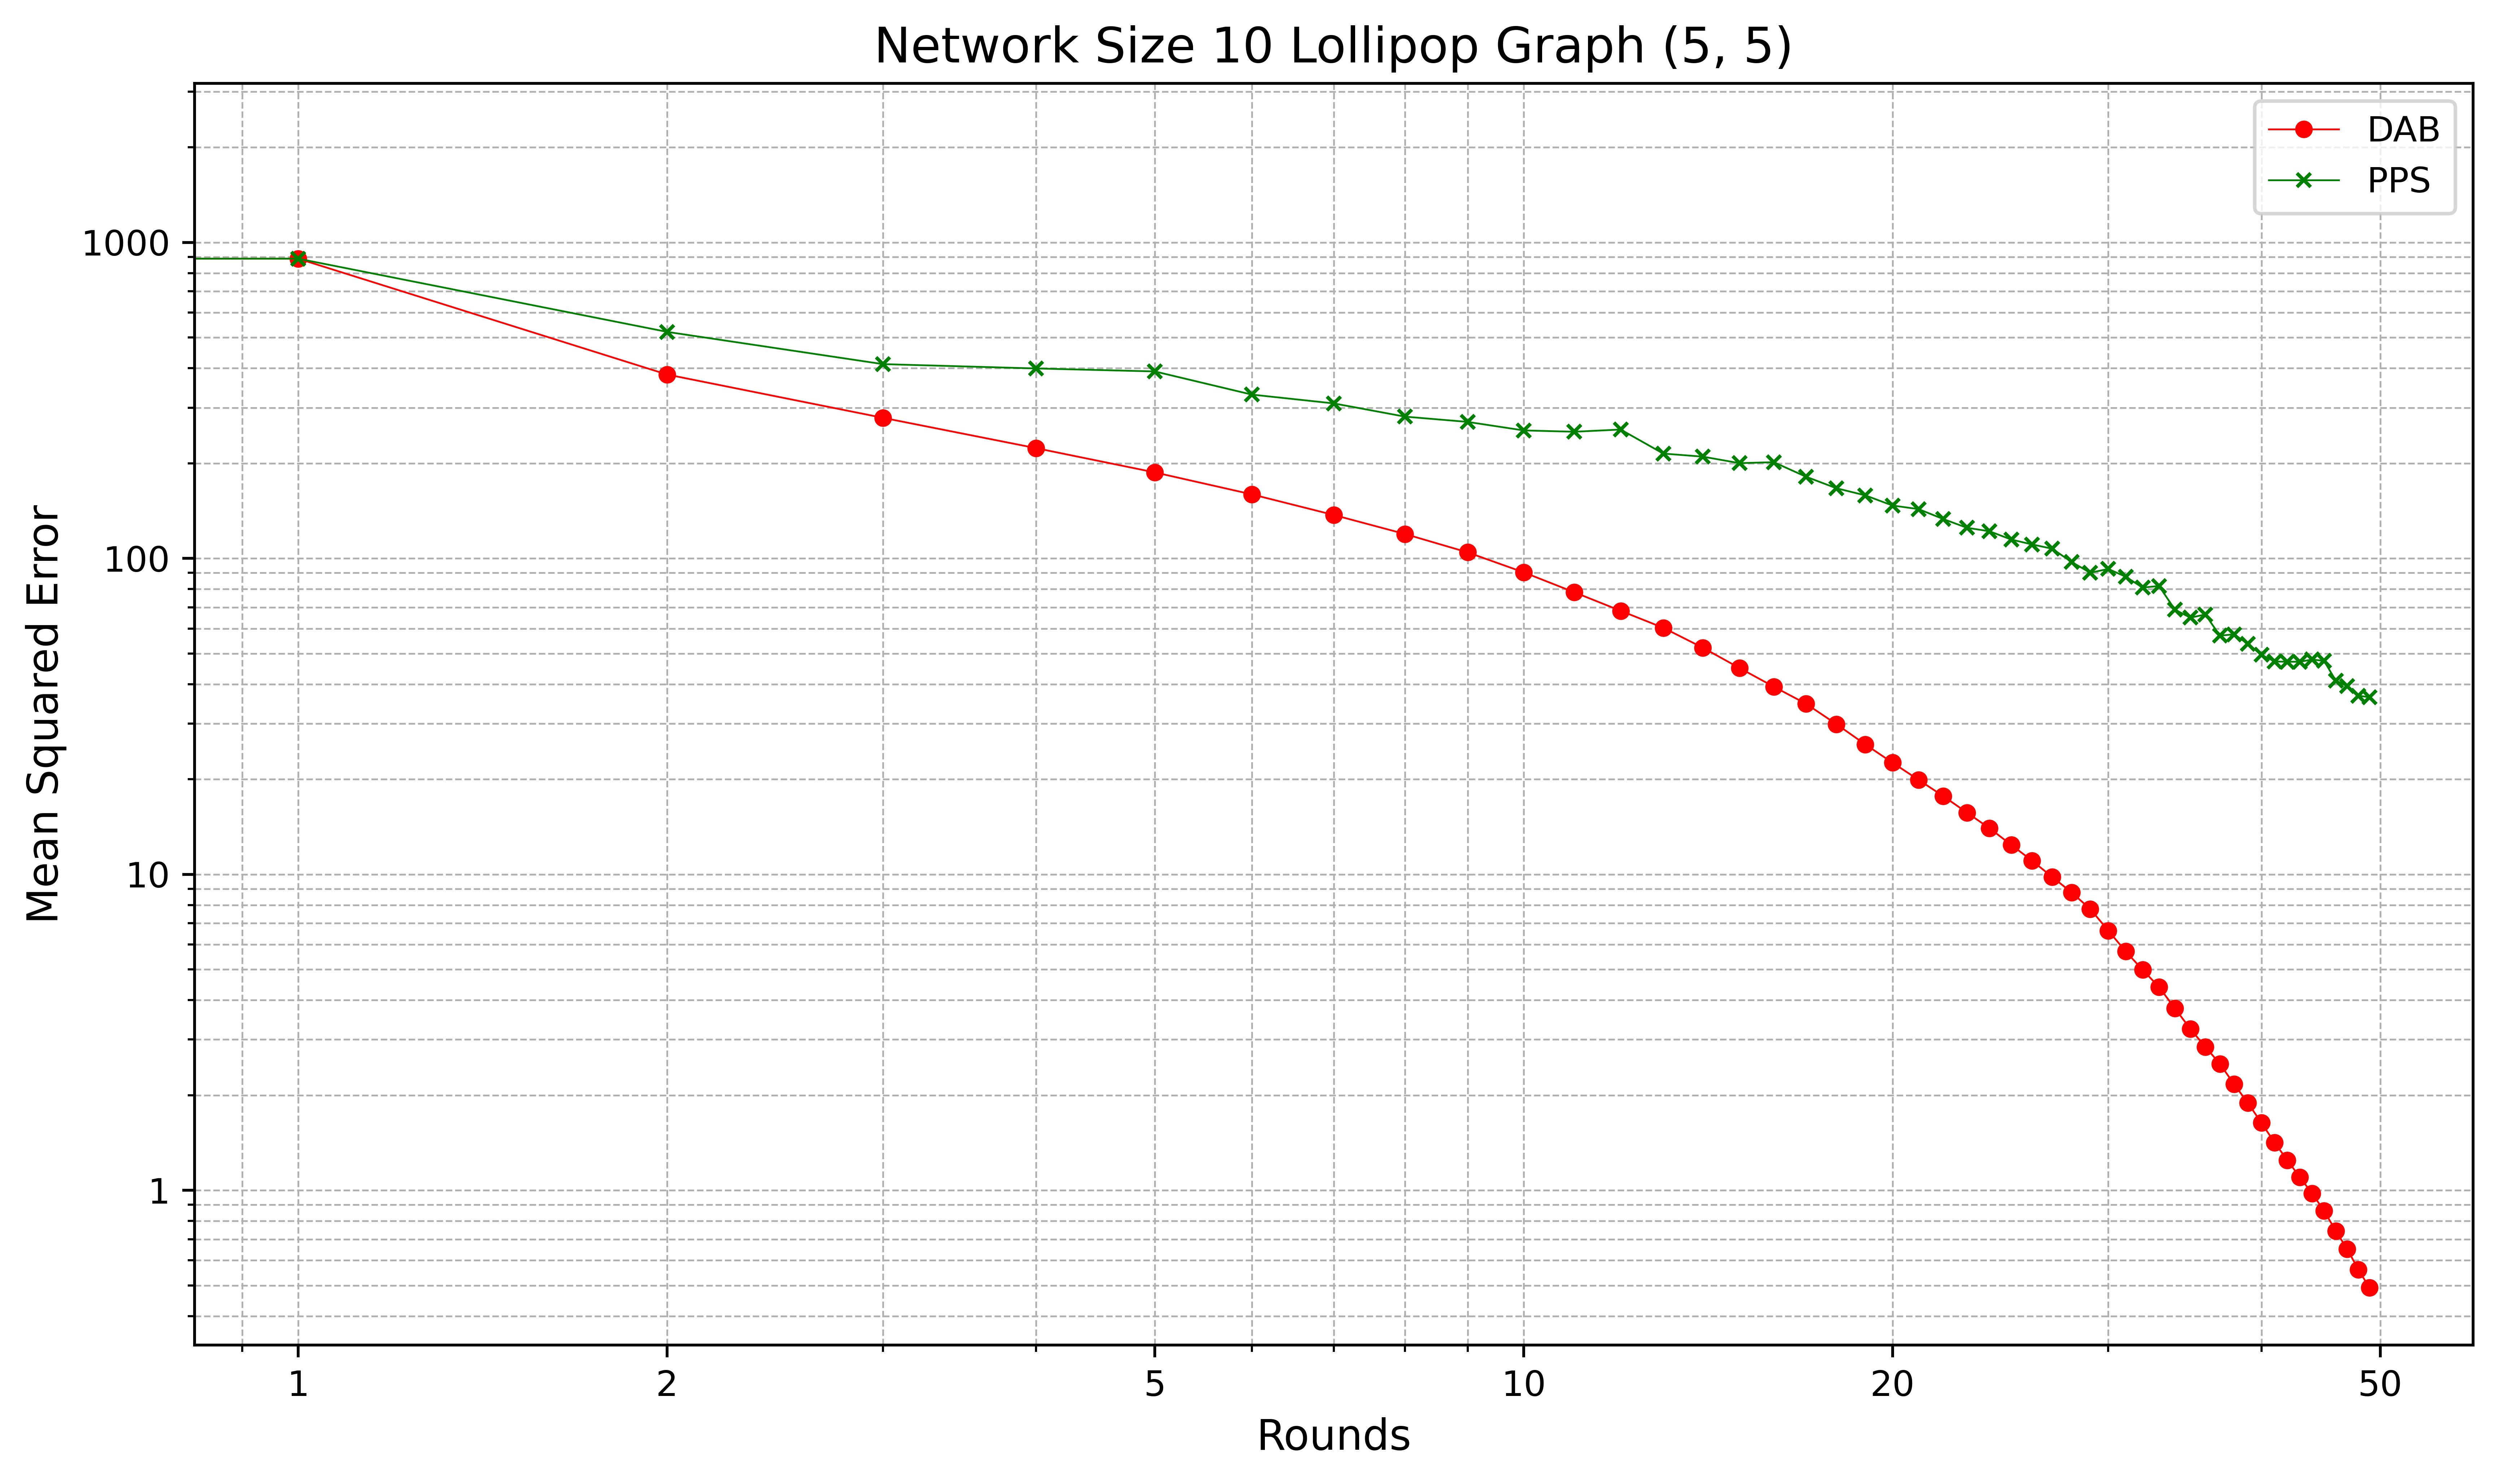
\includegraphics[scale=0.5]{figures/lollipopGraphSimulations/DAB_vs_PPS_LG_r50_n10.png}
    \caption{Lollipop graph: network size $10^{1}$ nodes $(5, 5)$}
    \label{fig:50+50lollipopgraph}
\end{figure}
\begin{figure}[H]
    \centering
    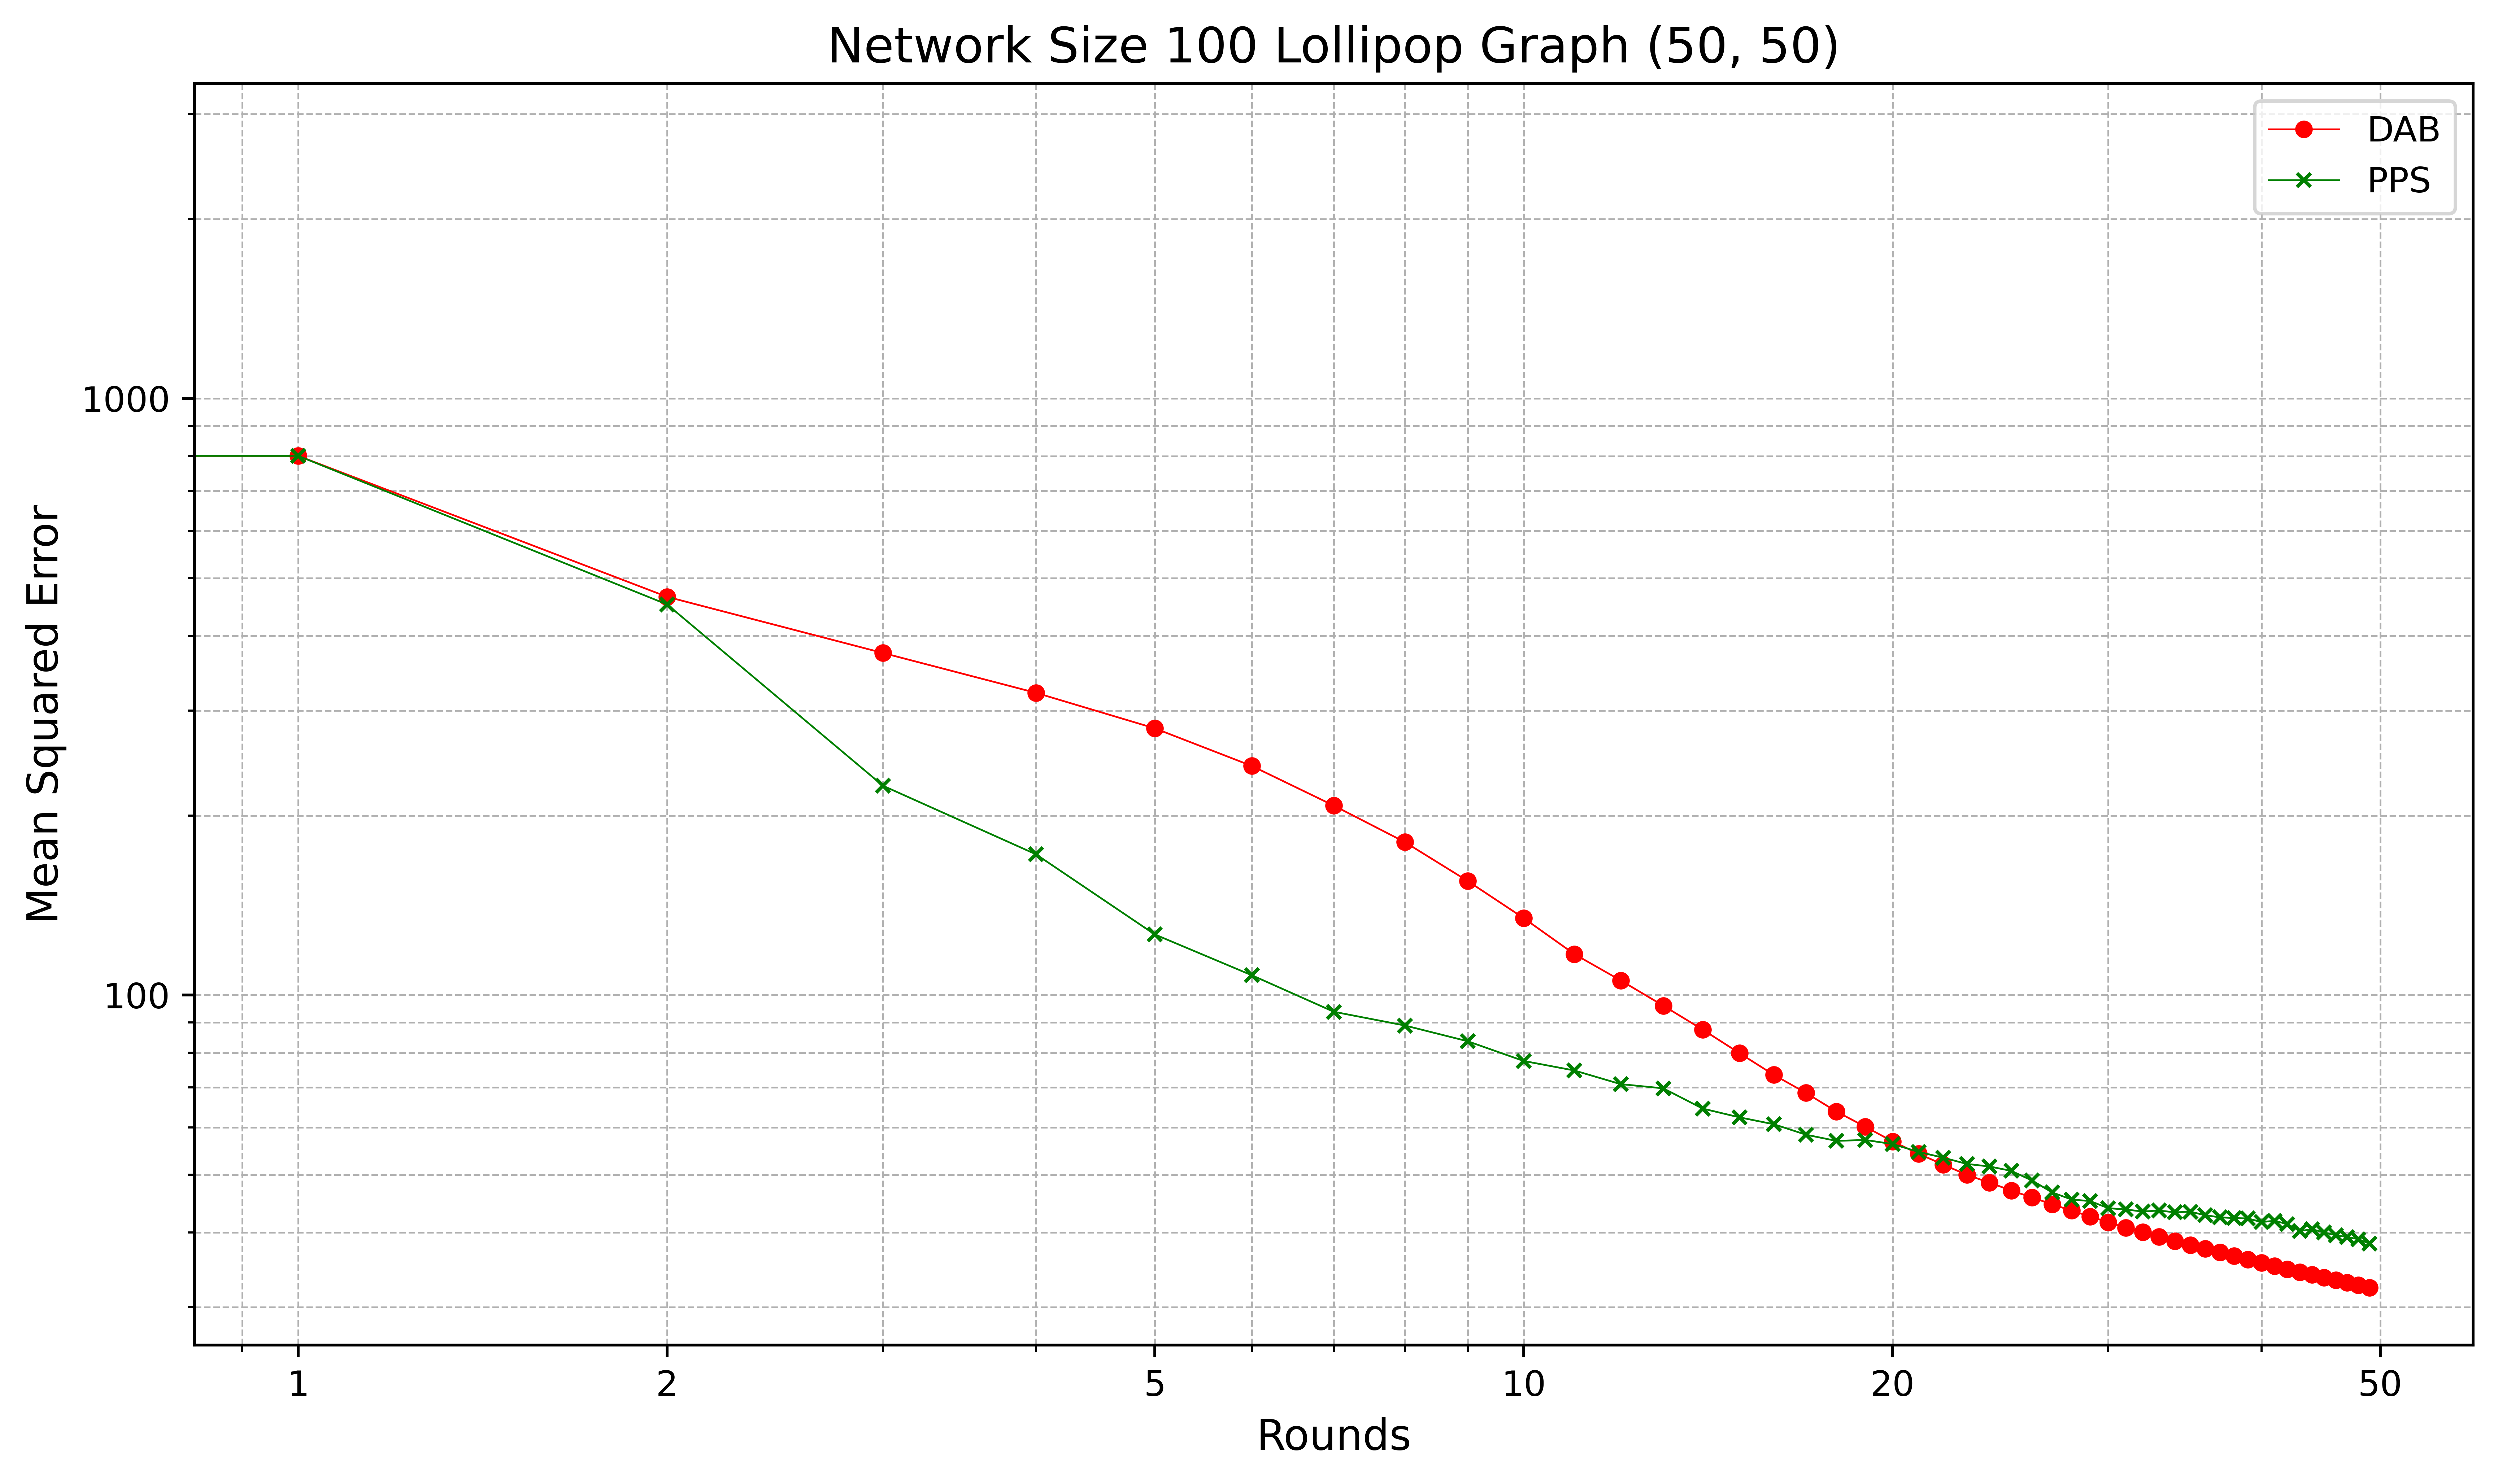
\includegraphics[scale=0.5]{figures/lollipopGraphSimulations/DAB_vs_PPS_LG_r50_n100.png}
    \caption{Lollipop graph: network size $10^{2}$ nodes $(50, 50)$}
    \label{fig:50+50lollipopgraph}
\end{figure}
\begin{figure}[H]
    \centering
    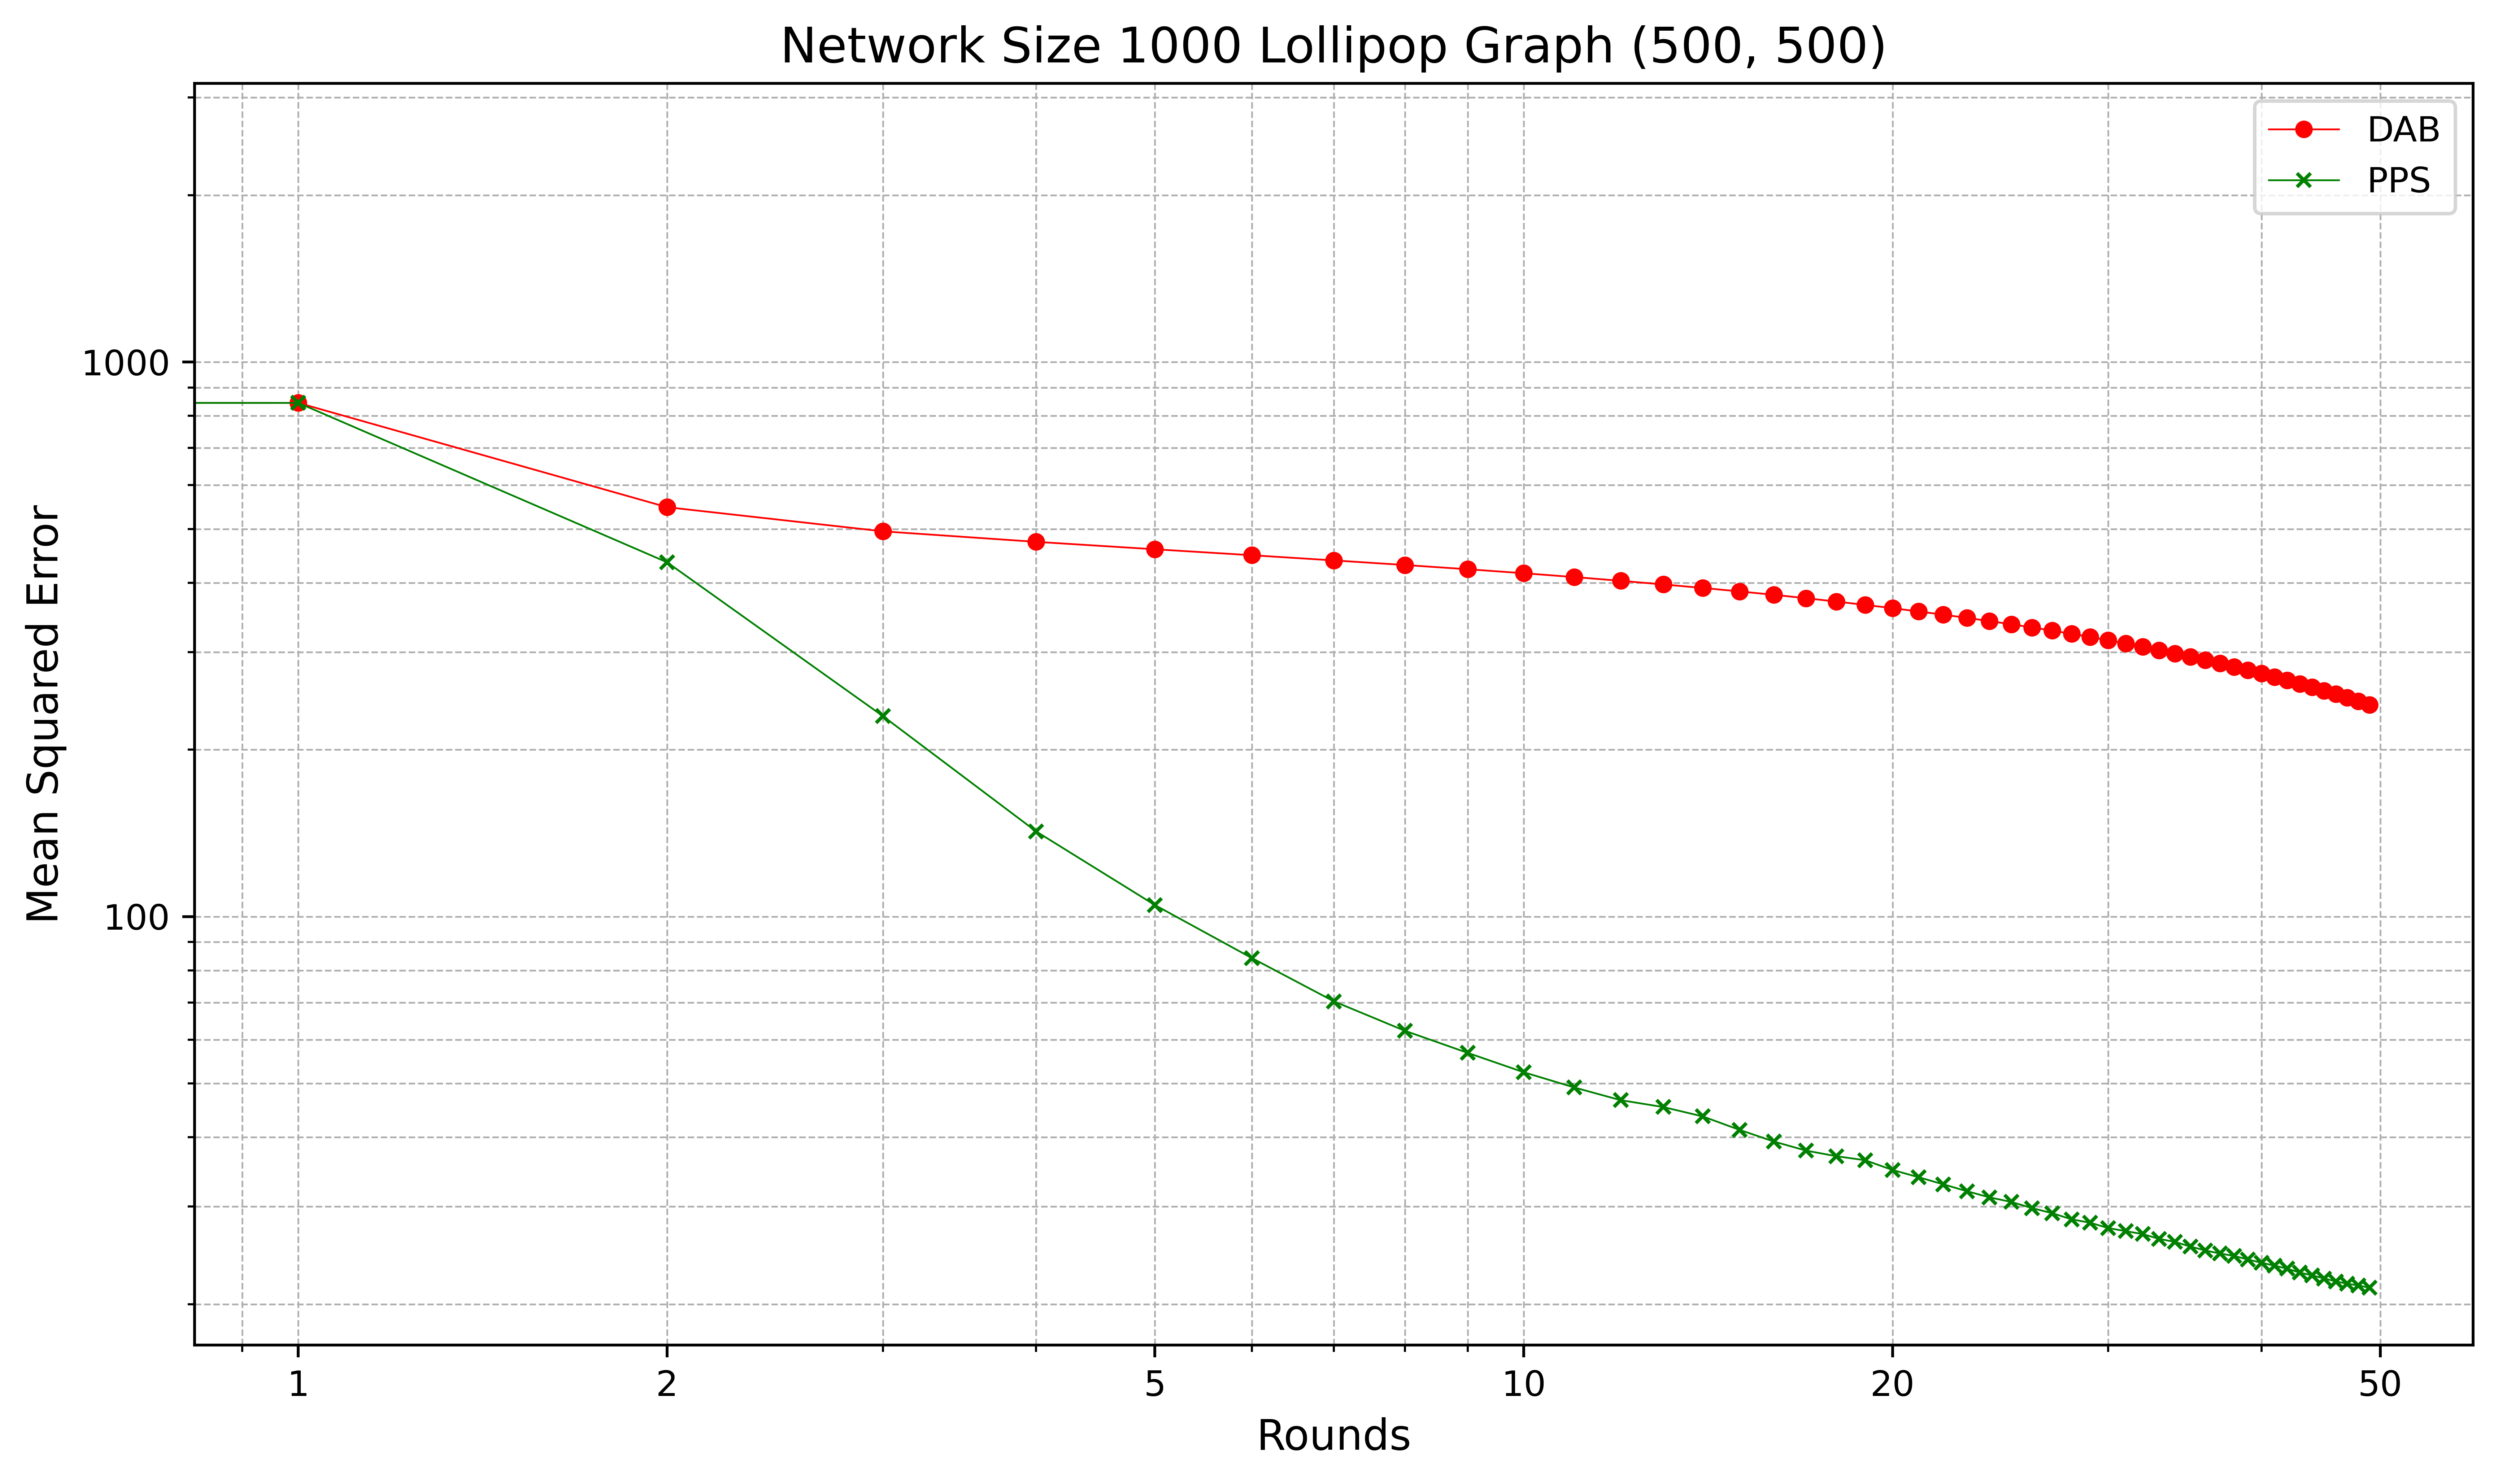
\includegraphics[scale=0.5]{figures/lollipopGraphSimulations/DAB_vs_PPS_LG_r50_n1000.png}
    \caption{Lollipop graph: network size $10^{3}$ nodes $(500, 500)$}
    \label{fig:500+500lollipopgraph}
\end{figure}
\begin{figure}[H]
    \centering
    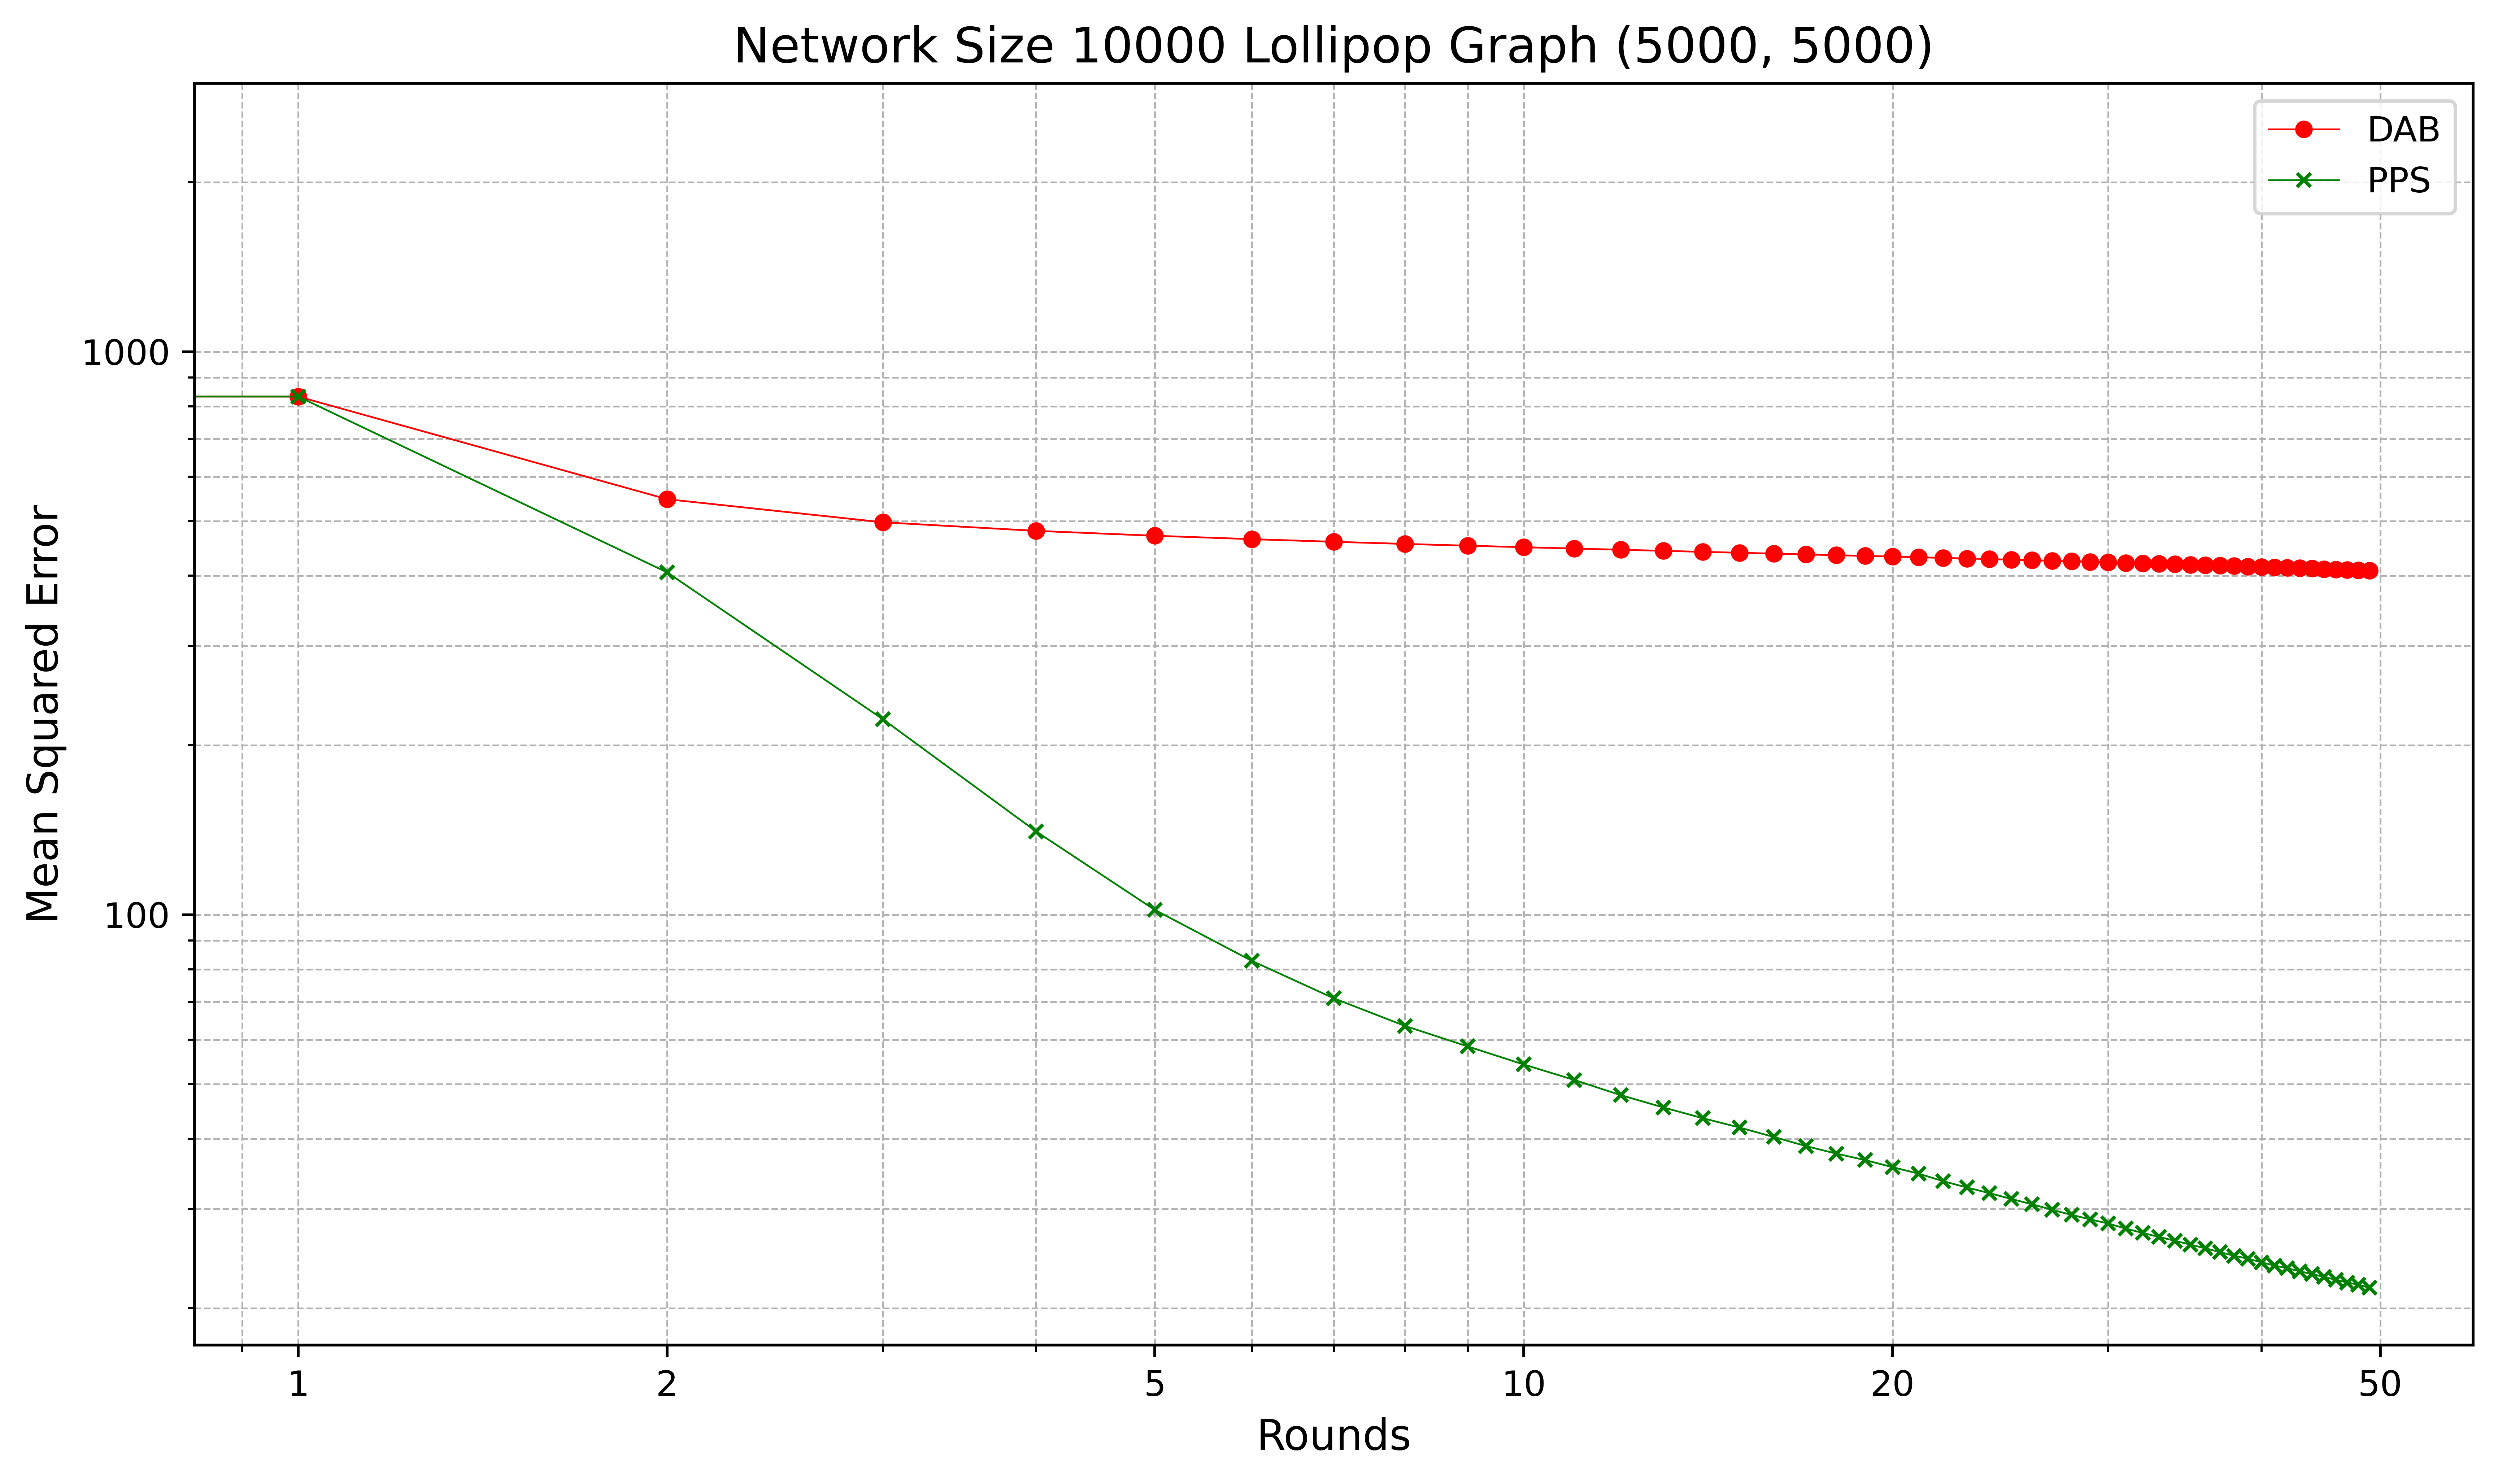
\includegraphics[scale=0.5]{figures/lollipopGraphSimulations/5000+5000/DAB_vs_PPS_LG_r50_n10000.png}
    \caption{Lollipop graph: network size $10^{4}$ nodes $(5000, 5000)$}
    \label{fig:5000+5000lollipopgraph}
\end{figure}
\begin{figure}[H]
    \centering
    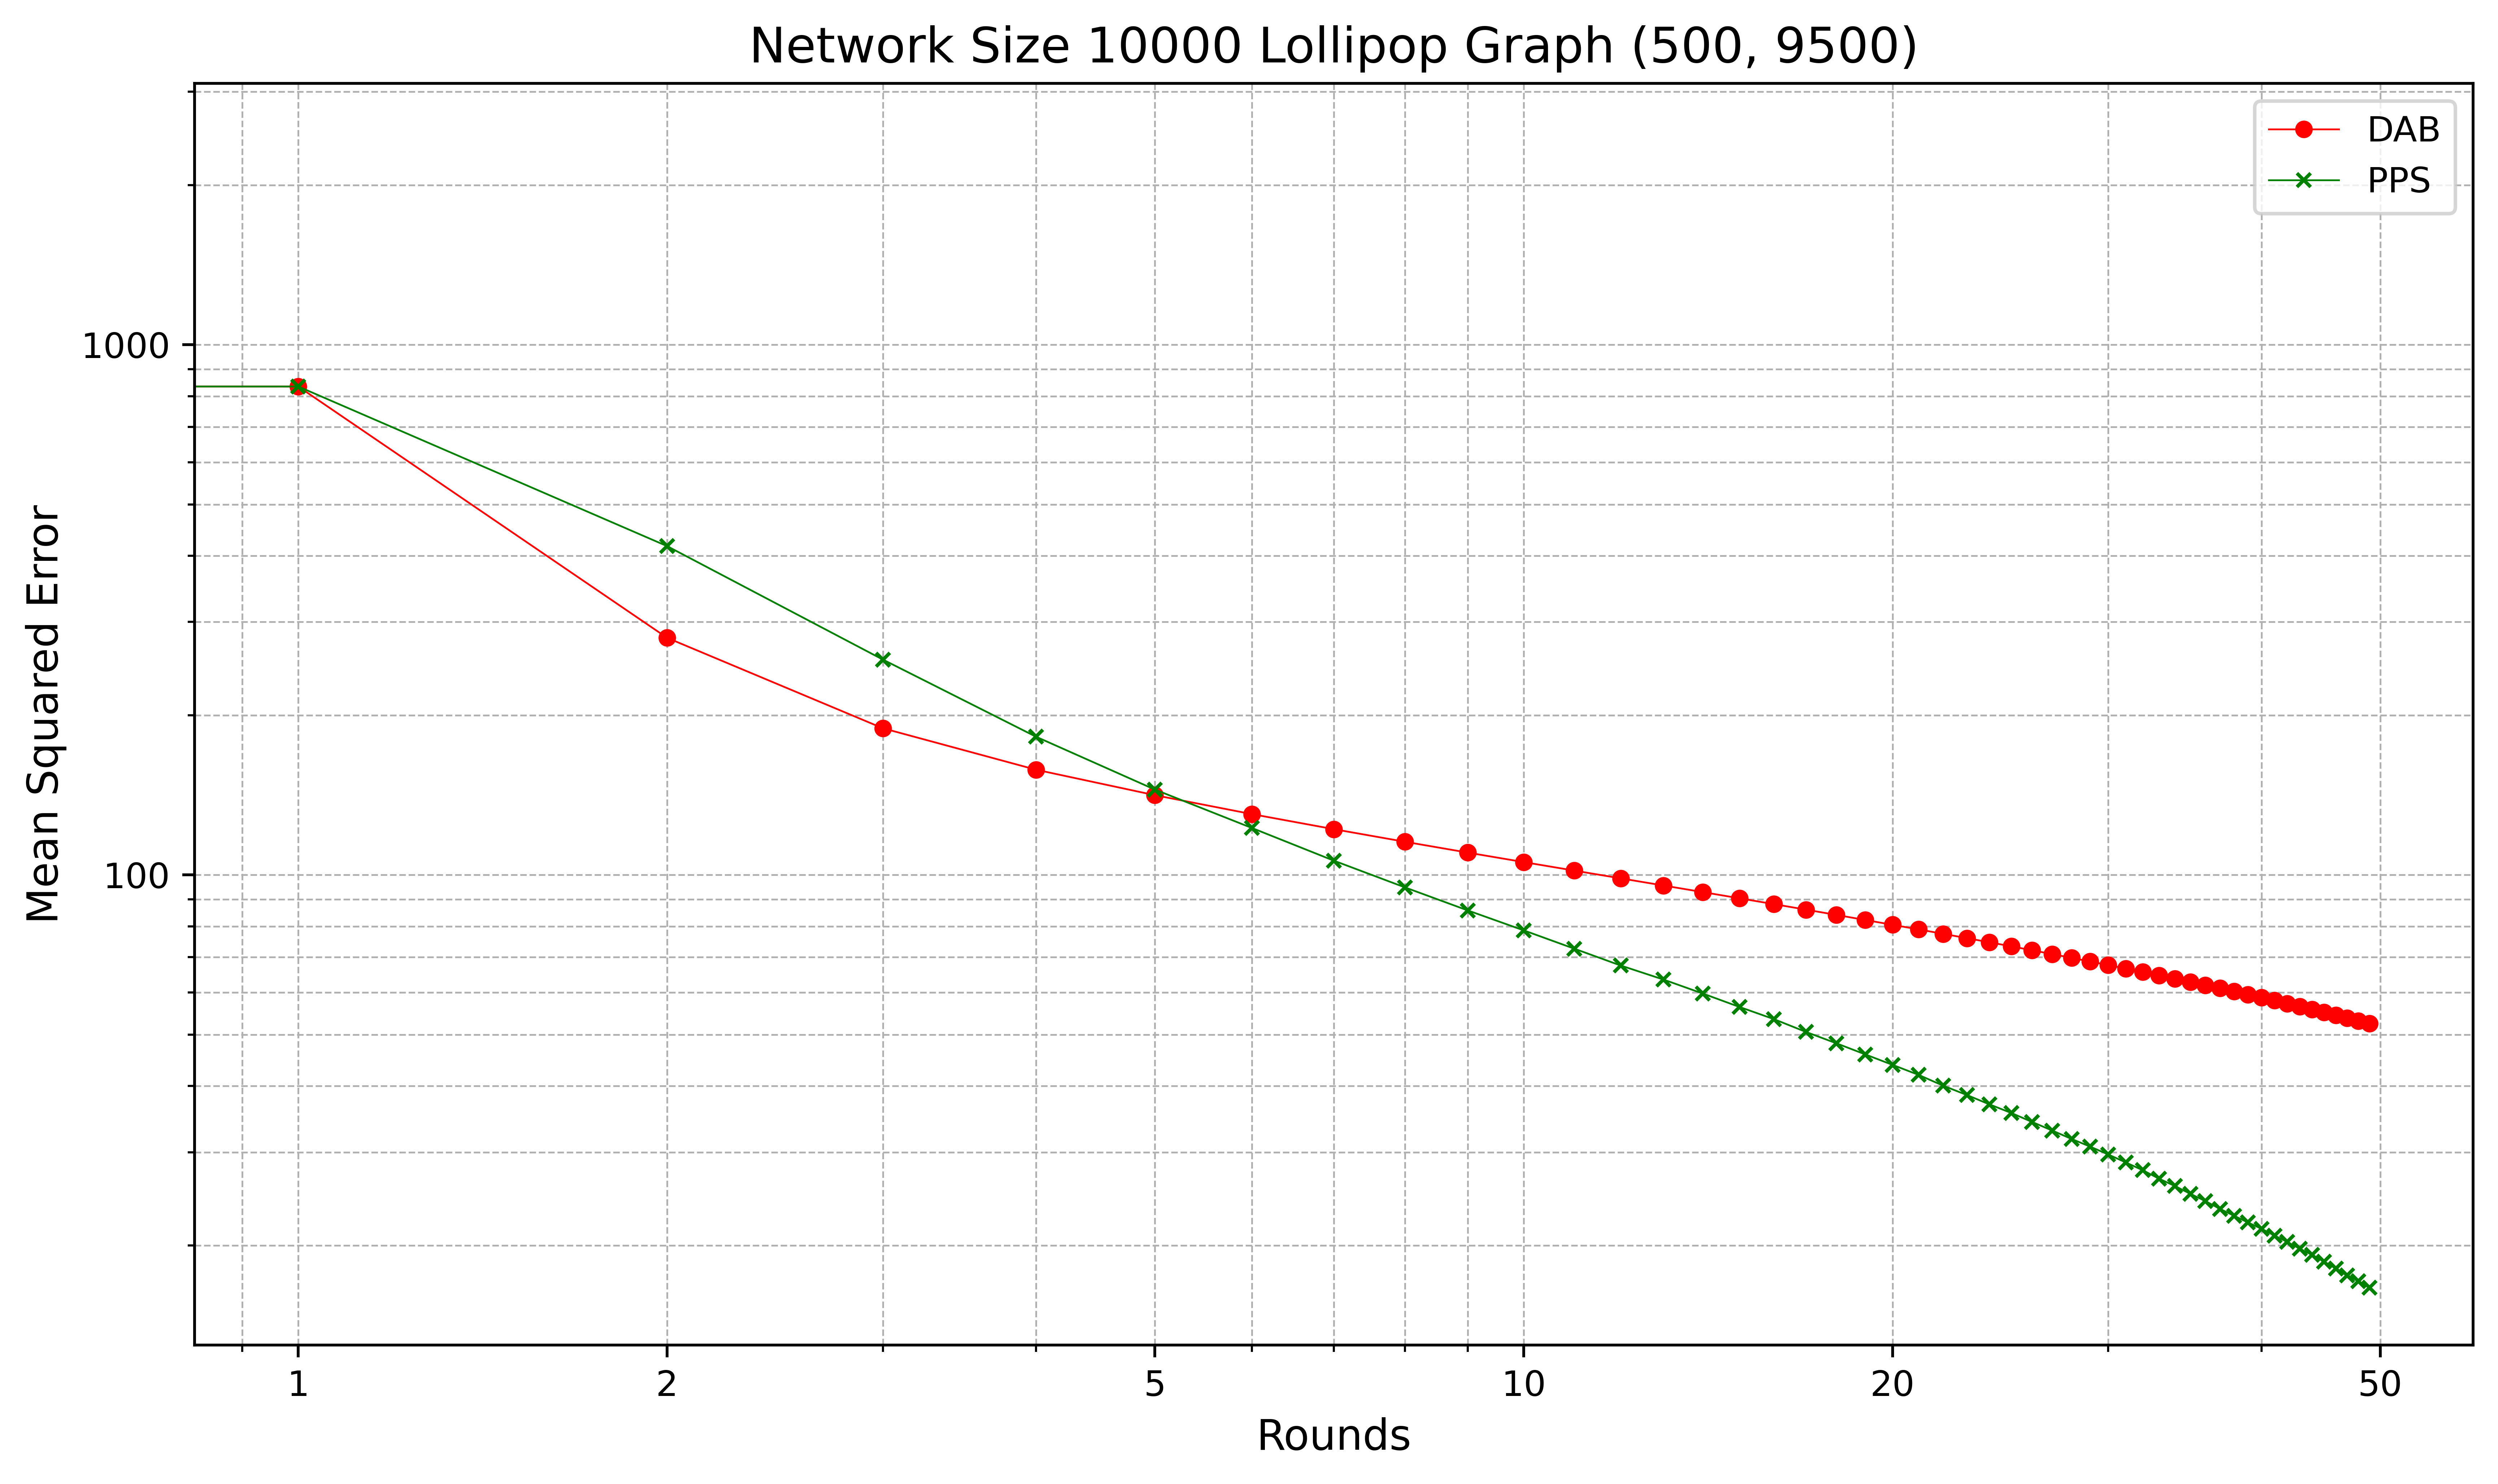
\includegraphics[scale=0.5]{figures/lollipopGraphSimulations/500+9500/DAB_vs_PPS_LG_r50_n10000.png}
    \caption{Lollipop graph: network size $10^{4}$ nodes $(500, 9500)$}
    \label{fig:500+9500lollipopgraph}
\end{figure}
\begin{figure}[H]
    \centering
    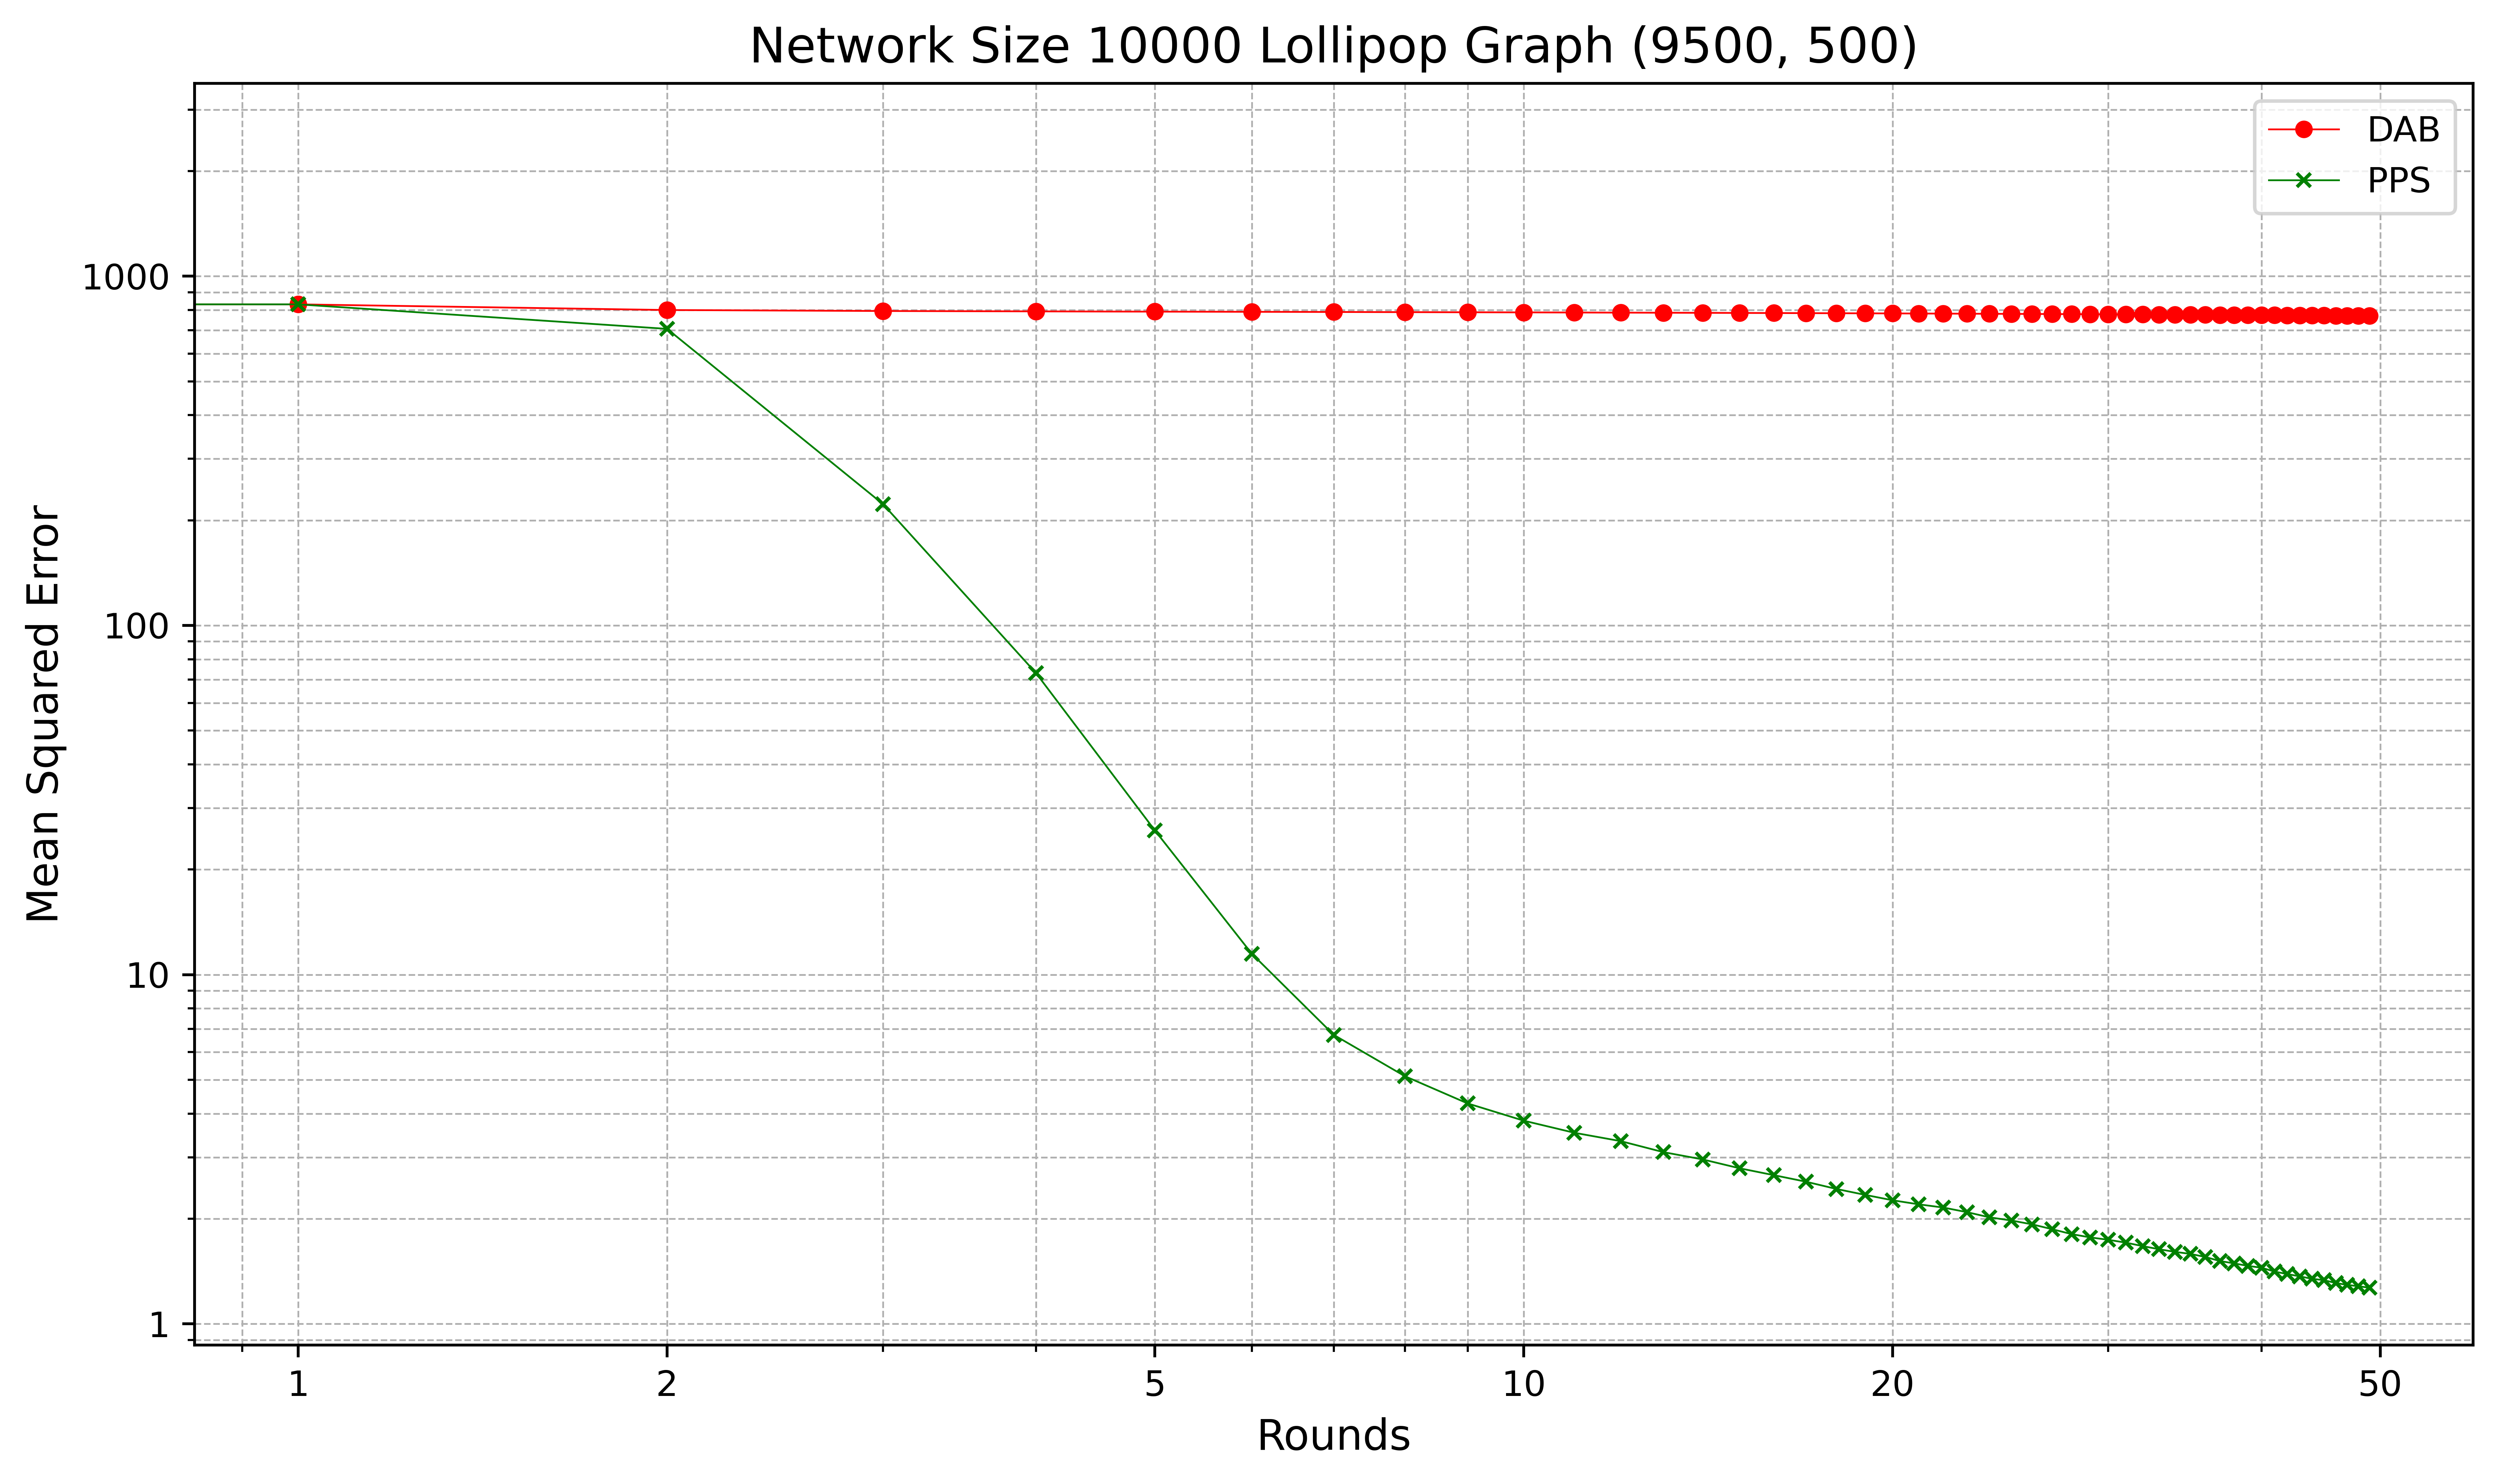
\includegraphics[scale=0.5]{figures/lollipopGraphSimulations/9500+500/DAB_vs_PPS_LG_r50_n10000.png}
    \caption{Lollipop graph: network size $10^{4}$ nodes $(9500, 500)$}
    \label{fig:9500+500lollipopgraph}
\end{figure}
    
    % If you want a list of your ToDos at the end of the document
    % don't forget to remove before submission!
    % place it somewhere in the document
\chapter*{ToDo Counters}
\newcounter{ct}%
To Dos: \arabic{todos}; \hspace{1em}%
\setcounter{ct}{0}%
\whiledo {\value{ct} < \value{todos}}%
{%
	\stepcounter {ct}%
    \ref{todo \thect}%
	\ifnum\value{ct} = \value{todos}{}\else{, }\fi
}

Parts to extend: \arabic{extends}; \hspace{1em}%
\setcounter{ct}{0}%
\whiledo {\value{ct} < \value{extends}}%
{%
	\stepcounter {ct}%
	\ref{extend \thect}%
	\ifnum\value{ct} = \value{extends}{}\else{, }\fi
}

Draft parts: \arabic{drafts}; \hspace{1em}%
\setcounter{ct}{0}%
\whiledo {\value{ct} < \value{drafts}}%
{%
	\stepcounter {ct}%
	\ref{draft \thect}%
	\ifnum\value{ct} = \value{drafts}{}\else{, }\fi
}

    \bibliographystyle{ieeetr}
    \bibliography{bib/main,bib/file2}
    % bibliography is not in the table of contents per default, add it manually
    % enable the \renewcommand for german header
    \renewcommand{\bibname}{References}
    \addcontentsline{toc}{chapter}{Bibliography}
    \newpage
    \thispagestyle{empty}
    \mbox{}


\end{document}
